
%\qquad Due quadratoni.
%
%\quad Un quadratone.
%
%\<SP> Uno spazio «normale».
%
%$\;$  Uno spazio spesso (5/8 di quadratone).
%
%$\>$  Uno spazio medio (2/9 di quadratone).
%
%$\.$  Uno spazio molto sottile (1/6 di quadratone).
%
%$\!$  Uno spazio negativo (-1/6 di quadratone).



%\documentclass[11 pt , letterpaper , twoside , openright ]{book}
\documentclass[11 pt , letterpaper , oneside ]{book}
\usepackage[T1]{fontenc}
\usepackage[utf8]{inputenc}
\usepackage{etoolbox}

\usepackage[ED=MEGEP-DyF, Ets=INP]{tlsflyleaf}


\usepackage[english]{babel}

\usepackage{caption} 
%\usepackage{subfig}

\usepackage{transparent}
\usepackage{eso-pic}
\usepackage{textcomp}
%\usepackage[acronym]{glossaries}

%the two package under these line are used for flow chart in chapter 2
\usepackage{tikz}
\usetikzlibrary{shapes.geometric, arrows}
\usetikzlibrary{mindmap} %for mind maps using tikz
\usepackage[procnames]{listings}  %scrivere codici
\usepackage{url} %generare collegamenti

\newcommand{\chapquote}[3]{\begin{quotation} \textit{#1} \end{quotation} \begin{flushright} - #2, \textit{#3}\end{flushright} } %writes quotes as chapter beginning

%%%%%%%%%%%%%%%%%%%%%%%%%%%%%%%%%%%%%%%%%%%%%%%%%%%%%%%

\usepackage{graphicx}
\usepackage{epsfig}
\usepackage{psfrag}
%\usepackage{subfigure}
\usepackage{subcaption}
% AMS bundle

\usepackage{amssymb}
\usepackage{amsmath}
\usepackage{amsfonts}
\usepackage{amsbsy}
\usepackage{amsthm}

\usepackage{bm}
\usepackage{epsfig}
\usepackage{epstopdf}
\usepackage{color}

\usepackage{caption}
\usepackage{booktabs}
\usepackage{float} % is needed by \begin{figure}[H]  to write [H]
\usepackage{mathrsfs}

\usepackage[linesnumbered]{algorithm2e}  %writing pseudocode

\usepackage[numbers, square]{natbib}

%%%%%%%%%%%%%%%%%%%%%%%%%%%%%%%%%%%%%%%%%%%%%%%%%%%%%%%

\newtheorem{theorem}{Theorem}[section]
\newtheorem{corollary}{Corollary}[section]

\newcommand{\bs}[1]{\boldsymbol{#1}}

\newcommand{\derp}[2]{\dfrac{\partial #1}{\partial #2}}

\def\rprth#1{\left( #1 \right)} %\prth{.} inside round parentesis
\def\sprth#1{\left[ #1 \right]} %\prth{.} inside square parentesis
\def\gprth#1{\left{ #1 \right}} %\prth{.} inside graph parentesis
\newcommand{\volb}{V_\beta} %\volb  volume of the fluid phase
\def\meani#1{{\left< #1 \right>}^{\beta}} %\mean{.} intrinsic average operator
\def\means#1{{\left< #1 \right>}} %\mean{.} superficial average operator
\newcommand{\vb}{\textbf{v}_{\beta}} %\vb velocity in the fluid
\newcommand{\ws}{\textbf{v}_{\sigma}} %\vb velocity in the fluid
\newcommand{\vbt}{\tilde{\textbf{v}}_{\beta}} %\vb velocity in the fluid
\newcommand{\pbt}{\tilde{p}_{\beta}} %\pbt spatial fluctuation pressure in the fluid
\newcommand{\vbmi}{\meani{\textbf{v}_{\beta}}} %\vbmi intrinsic average velocity of fluid phase 
\newcommand{\vbms}{\means{\textbf{v}_{\beta}}} %\vbms superficial average velocity of fluid phase 
\newcommand{\rhos}{\rho_{\sigma}} %\ density of the solid phase
\newcommand{\pb}{p_{\beta}} %\pb pressure of fluid phase
\newcommand{\pbmi}{\meani{p_{\beta}}} %\pbmi intrinsic average pressure of fluid phase 
\newcommand{\pbms}{\means{\textbf{v}_{\beta}}} %\vbms superficial average velocity of fluid phase 
\newcommand{\nub}{\nu_{\beta}} %\nub cinematic viscosity of fluid phase
\newcommand{\mub}{\mu_{\beta}} %\mub dynamic viscosity of fluid phase
\newcommand{\nbs}{\mathbf{n}_{\sigma \beta}} %\mub dynamic viscosity of fluid phase

\newcommand{\Red}[1]{{\textcolor{red}{#1}}}
\newcommand{\Blue}[1]{{\textcolor{blue}{#1}}}

\newcommand{\vs}[1]{\vspace{ #1 cm}}
\newcommand{\hs}[1]{\hspace{ #1 cm}}

%%%%%%%%%%%%%%%%%%%%%%%%%%%%%%%%%%%%%%%%%%%%%%%%%%%%%%%

\input frontpage

%%%%%%%%%%%%%%%%%%%%%%%%%%%%%%%%%%%%%%%%%%%%%%%%%%%%%%%
% with this you compile only one chapter and not the all document
%\includeonly{chapter_1/chapter_1} 
%%%%%%%%%%%%%%%%%%%%%%%%%%%%%%%%%%%%%%%%%%%%%%%%%%%%%%%





\begin{document}
	\makeflyleaf


%\include{contorno/dediche}
\chapter*{Abstract}

Any natural surface is in essence non-smooth, consisting of more or less regular roughness and/or mobile structures of different scales. From a fluid mechanics point of view, these natural surfaces offer better aerodynamic performances when they cover moving bodies, in terms of drag reduction, lift enhancement or control of boundary layer separation; this has been shown for boundary layer or wake flows around thick bodies. The numerical simulation of microscopic flows around "natural" surfaces is still out of reach today. Therefore, the goal of this thesis is to study the modeling of the apparent flow slip occurring on this kind of surfaces, modeled as a porous medium, applying Whitaker's volume averaging theory. This mathematical model makes it possible to capture details of the microstructure while preserving a satisfactory description of the physical phenomena which occur. 

The first chapter of this manuscript provides an overview of previous efforts to model these surfaces, detailing the most important results from the literature. The second chapter presents the mathematical derivation of the volume-averaged Navier-Stokes equations (VANS) in a porous medium. In the third chapter the flow stability at the interface between a free fluid and a porous medium, formed by a series of rigid cylinders, is studied. The presence of this porous layer is treated by including a drag term in the fluid equations. It is shown that the presence of this term reduces the rates of amplification of the Kelvin-Helmholtz instability over the whole range of wavenumbers, thus leading to an increase of the wavelength of the most amplified mode. In this same context, the difference between the isotropic model and a tensorial approach for the drag term was evaluated, to determine the most consistent approach for the study of the stability of this type of flows. This has led to the conclusion that the most relevant model is the one using the apparent permeability tensor. In the following chapter, based on this last result, the apparent permeability tensor, based on over one hundred direct numerical simulations carried out over microscopic unit cells, has been identified for a three-dimensional porous medium consisting of rigid cylinders. In these configurations the tensor varies according to four parameters: the Reynolds number, the porosity and the orientation of the average pressure gradient (the latter defined by two Euler angles). This parameterization makes it possible to capture local three-dimensional effects. This database has been set up to create, based on a kriging-type approach, a behavioral meta-model for estimating all the components of the apparent permeability tensor.

In the fifth chapter, simulations of the VANS equations are carried out on a macroscopic scale after the implementation of the meta-model, and this allows reasonable computing times. The validation of the macroscopic approach is performed on a flow in a closed cavity covered with a porous layer and a comparison with the results of a very precise DNS, homogenized a posteriori, shows a very good agreement and demonstrates the relevance of the approach. The next step has been the study of the passive control of the separation of the flow past a hump which is placed on a  porous wall, by the same macroscopic VANS approach.  Finally, general conclusions and possible directions of research in the field are presented in the last chapter.
\chapter*{Résumé}

Le nombre de caractères ne doit pas être supérieur à 4000. 
Les résumés français et anglais doivent tenir tous deux en 4ème de couverture de votre manuscrit, et les résumés déposés ici doivent être identiques à ceux du manuscrit.
Presque toutes les surfaces existant dans la Nature ne sont pas lisses, elles ont des rugosités plus ou moins régulières et/ou des structures mobiles à différentes échelles
Ces surfaces ont des meilleures performances aérodynamiques (réduction de traînée, augmentation de la portance, contrôle de séparation…) et cela a été prouvé sur des cas comme des couches limites et des corps épais.

Faire des calculs à l’échelle microscopique n’est pas faisable, de ce fait nous voulons trouver une manière de modéliser le glissement apparent sur ces surfaces (modélisé comme un milieu poreux) utilisant la théorie de Moyenne-Volumique de Whitaker [134].
Ce modèle mathématique nous permet de représenter en moyenne les détails de la micro-structure sur ces surfaces mais cela donne encore une bonne description des phénomènes.
Le premier chapitre de ce manuscrit donne un panoramique des efforts précédents sur la modélisation de ces surfaces, et présente les indications plus importantes qui sont tirées de la bibliographie.

Le deuxième chapitre présente la dérivation mathématique des équations de Navir-Stokes Moyenne en Volume (VANS) dans un milieu poreux.
Dans le troisième chapitre nous étudions la stabilité de l’écoulement à l’interface entre un fluide libre et un milieu poreux, faite d'une série de cylindres rigides.
La présence de cette couche poreuse a été traitée avec un terme de traînée dans les équations de fluides.
On montre que la présence de ce terme reduit les facteurs d’amplification de l’instabilité des Kelvin-Helmholtz sur toute la gamme de nombre d’ondes et ainsi augmente la longueur d’onde du mode le plus amplifie.
Dans le même contexte on a calculé la différence entre un modèle isotrope de traînée et une approche tensorielle pour le terme de traînée, dans le but de comprendre qu’elle était l’approche plus solide pour le calcul de stabilité. Notre conclusion était que le modèle qu'utilise le tenseur de perméabilité apparent est le meilleur choix.
Basé sur ce résultat, dans le chapitre quatre nous avons calculé numériquement le tenseur de perméabilité apparent, pour un milieu poreux 3D constitué de cylindres rigides, avec les problèmes de fermeture dérivées avec les VANS. 
En effet ce tenseur vari avec le nombre de Reynolds, l’orientation du gradient de pression moyenne est la porosité. 
Les deux angles d’Euler qui définissent l’orientation du gradient de pression sont inclus dans le modèle pour capturer le possible effet 3D.  Partant de cette base de données, une interpolation de kriging a été utilisée pour obtenir une estimation de tous les composants du tenseur pour chaque paramètre d’entrée.

Dans le dernier chapitre nous montrons des résultats basés sur ce méta modèle; l’utilisation de ce modèle d’ordre réduit avec un code numérique basé sur les équations VANS à l’échelle macroscopique, permet de maintenir les temps de calcul entre des niveaux raisonnable.
Pour validé cette description macroscopique nous comparons la simulation d'une cavité ferme avec une couche poreuse, avec les VANS et avec les résultats d’un DNS homogénéisé a posteriori. 
Cette comparaison montre un bon accord entre les deux modèles.
Avec la même description macroscopique nous étudions la possibilité d’utiliser les équations VANS pour faire des simulations d’écoulements détachés et constater si cette couche poreuse peut contrôler cette séparation.
Enfin, le dernier chapitre présente la conclusion de ce travail et la possible direction de recherche dans ce domaine.
%%\include{contorno/nomenclatura}

\tableofcontents
\listoffigures
\listoftables

\chapter{Poroelastic natural coatings}

\chapquote{Nature is the source of all true knowledge. She has her own logic, her own laws, she has no effect without cause nor invention without necessity}{}{Leonardo Da Vinci}

\section{Biomimetics of poroelastic coatings}

Usually when someone is asked to imagine some "rapid" object as an airplane, a boat or a car, the common sense lead us to think about it as the smoothest as possible and, most of the time, shiny.
But if we look around, the nature seems not to agree with the previous statement.
In fact most of the surfaces in nature are not smooth at all, they almost always present some kind more or less regular arrangement of discontinuities at various length scales.
Since Nature have had a very large time-span to optimize this kind of surfaces we can be very certain that they are the best possible option.
One should pinpoint that the non smoothness of these surfaces can be connected to some other biological functions rather than pure fluid dynamic performance, and of course it can be the case.

With that in mind we want to show the reader some of the most notably examples of "natural" aerodynamic surfaces.

Probably the most notable example is the shark skin, in figure \ref{fig:shark} a segment of the skin is depicted, as if appears to be, under the microscope.

\begin{figure}[h]
	\centering
	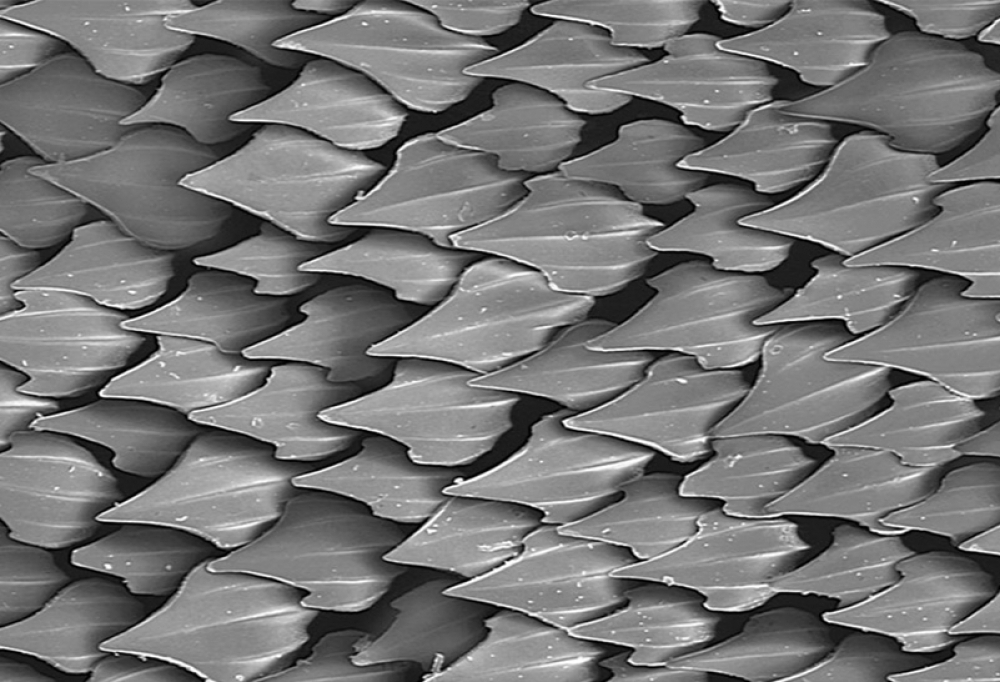
\includegraphics[width=0.6\linewidth]{chapter_1/shark}
	\caption{Microscope enlarged picture of the shark skin}
	\label{fig:shark}
\end{figure}

The enlargement show that the surface is made up by a series of overlapped denticles, and experiment shows that they can move and interact with the flow.

The shark "technology" has somehow been applied by Speedo$^{\circledR}$; they have fabricated their famous swimming suits with a surface that mimic the roughness of sharks; and they happen to break multiples world records.
But it seems that this controversial swimmers performance was due to the fact that they compress the body giving to the swimmer a more and streamlined shape.
But even thought the company has been publicized their product as it was a synthetic shark skin, \citet{Oeffner785} has shown that the texture of their swimming suits is somehow different from the shark dermal structure.
In they work the authors have performed swimming experiment with a flat plate with different surfaces and they did not found significant speed enhancement with the swimsuit surfaces; but the measurements with real shark skin on the contrary give an appreciable improvement in the performance.


Poroelastic surfaces find also applications in aeroacoustics, in fact owls are well known for their particularly silent flight, especially in the high frequency spectrum.
This characteristic is crucial for the owl in order to be able to capture his preys.
Obviously it has inspired the scientific community to study their feathers configuration and shape.

\begin{figure}[h]
	\centering
	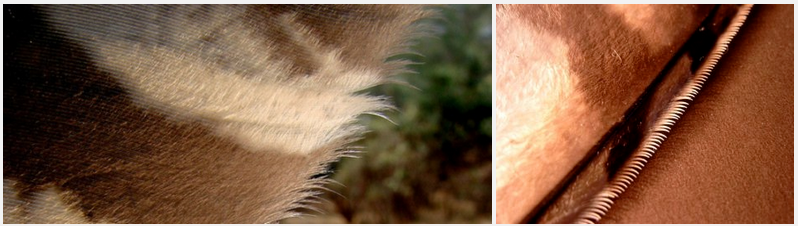
\includegraphics[width=0.8\linewidth]{chapter_1/howl}
	\caption{Feathers in owl's wing. Left: trailing edge. Right: leading edge. The difference in shape, mechanical properties, as rigidity, between the leading and trailing edge is a consequence of the different flow regimes in the wing}
	\label{fig:owl}
\end{figure}
 
Multiple authors show promising result in characterizing the acoustic properties of the owl skin and their physical mechanism.
In particular \citet{lilley1998} present three main characteristic of the owl that can suppress its airborne noise: the feathers leading edge shaped like a comb; the trailing edge that form a fringe, and the presence of multiple "filaments" in the bottom surface of wing and legs.
In the same work the authors also present some experimental and empirical evidence on the aeroacoustics mechanism behind the three elements above.

Another examples of work in the field of owls acoustic is the one by \citet{jaworski2013aerodynamic} in which the authors study the acoustic scattering problem of a poroelastic half-plane hit by an incident plane wave.
This configuration has been used as an analogy with the owl wing, it try to explain how the properties of this surface can suppress the noise.
They conclude that the combined effects of elasticity and porosity can produce weakest noise amplification.

Recent computational simulation made by \citet{rao2017owl} confirm that the leading edge shape of the feathers truly suppress noise and enhance the lift generation.

Bioinspired aerodynamic surfaces include another peculiar example in the butterflies wings.
In figure \ref{fig:butterfly} the surface of a "Peacock butterfly" is enlarged in order to show the multiple scales involved; the wing structure present firstly a series of overlapped scales similar to the shark, but looking closely we can observe that the singles scales have a complicated permeable structure.

\begin{figure}[h]
	\centering
	\begin{subfigure}[b]{0.3\textwidth}
		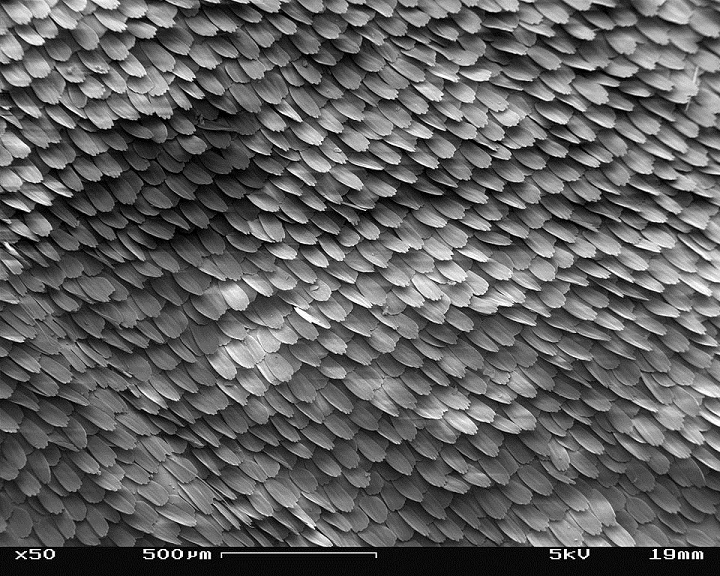
\includegraphics[width=\textwidth]{chapter_1/butterfly}
		\caption{Magnification 50x}
		\label{fig:b50}
	\end{subfigure}
	~ %add desired spacing between images, e. g. ~, \quad, \qquad, \hfill etc. 
	%(or a blank line to force the subfigure onto a new line)
	\begin{subfigure}[b]{0.3\textwidth}
		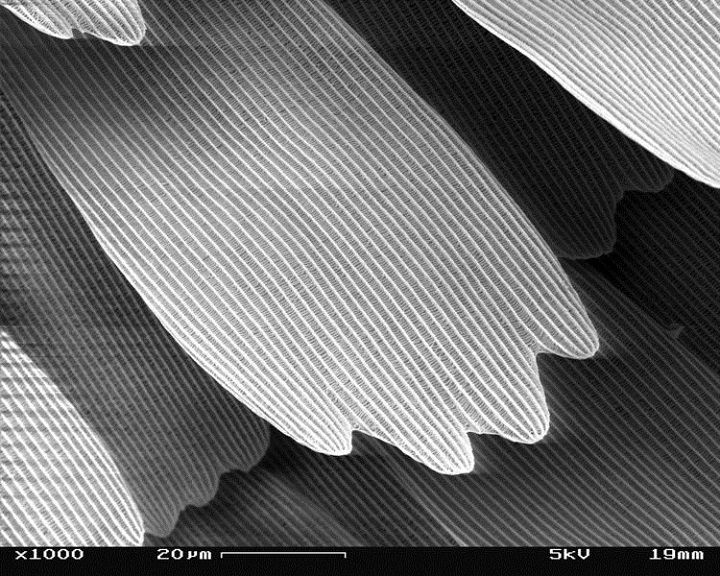
\includegraphics[width=\textwidth]{chapter_1/butterfly2}
		\caption{Magnification 1000x}
		\label{fig:b1000}
	\end{subfigure}
	\begin{subfigure}[b]{0.3\textwidth}
		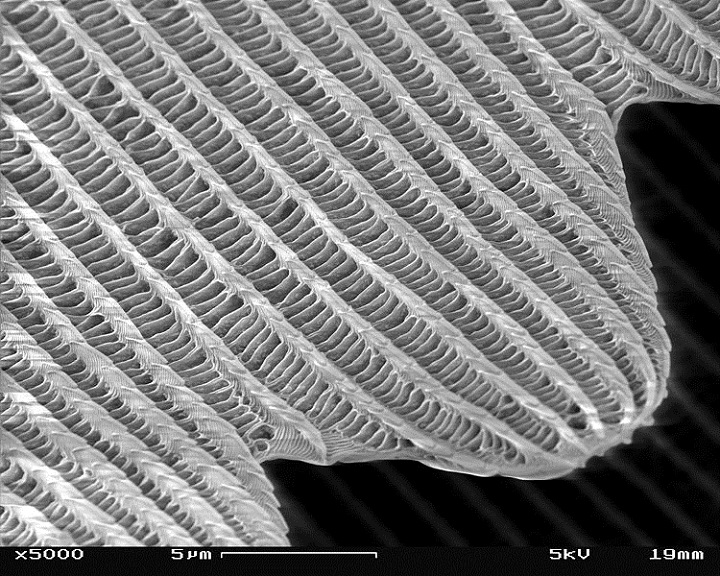
\includegraphics[width=\textwidth]{chapter_1/butterfly3}
		\caption{Magnification 5000x}
		\label{fig:b5000}
	\end{subfigure}
	\caption{Peacock butterfly wing surface using Scanning Electron Microscopy.  Images from wikimedia.org}
	\label{fig:butterfly}
\end{figure}

The work of \citet{slegers2017beneficial} study the effect of such porous structure in the flight performance of butterflies.
Using cameras to measure the kinematics of their flight, they can compute their efficiency to "climb" (generate lift) and the stroke amplitude and frequency.
The authors conclude that the porous structure of their wing gives a boost in climbing efficiency about $30\%$; that results clearly stress out the importance of poroelastic layer coating of the wings. 
Even though the butterfly flight aerodynamic is extremely complex, it seems clear that the peculiar structure of the wings surface is critical for their aerodynamic performances \citet{srygley2002unconventional}.

The last example will be super-hydrophobic surfaces; these surfaces are water repellent, it means that the water can slide over with much less resistance resulting in very small values of wettability.
This behavior is caused by the microscopic structure that forms the surface (see figure \ref{fig:lotus}), in fact the rugosities are arranged in a more or less regular way in order to be able to capture air pockets that rest inside this structures.
These air inclusion provoke an effective slip at the air-liquid interface that cause the drag reduction; they also change the contact angle of droplets.
The work of \citet{bottaro2003effect} summarize the above aspect and their applications.

\begin{figure}[h]
	\centering
	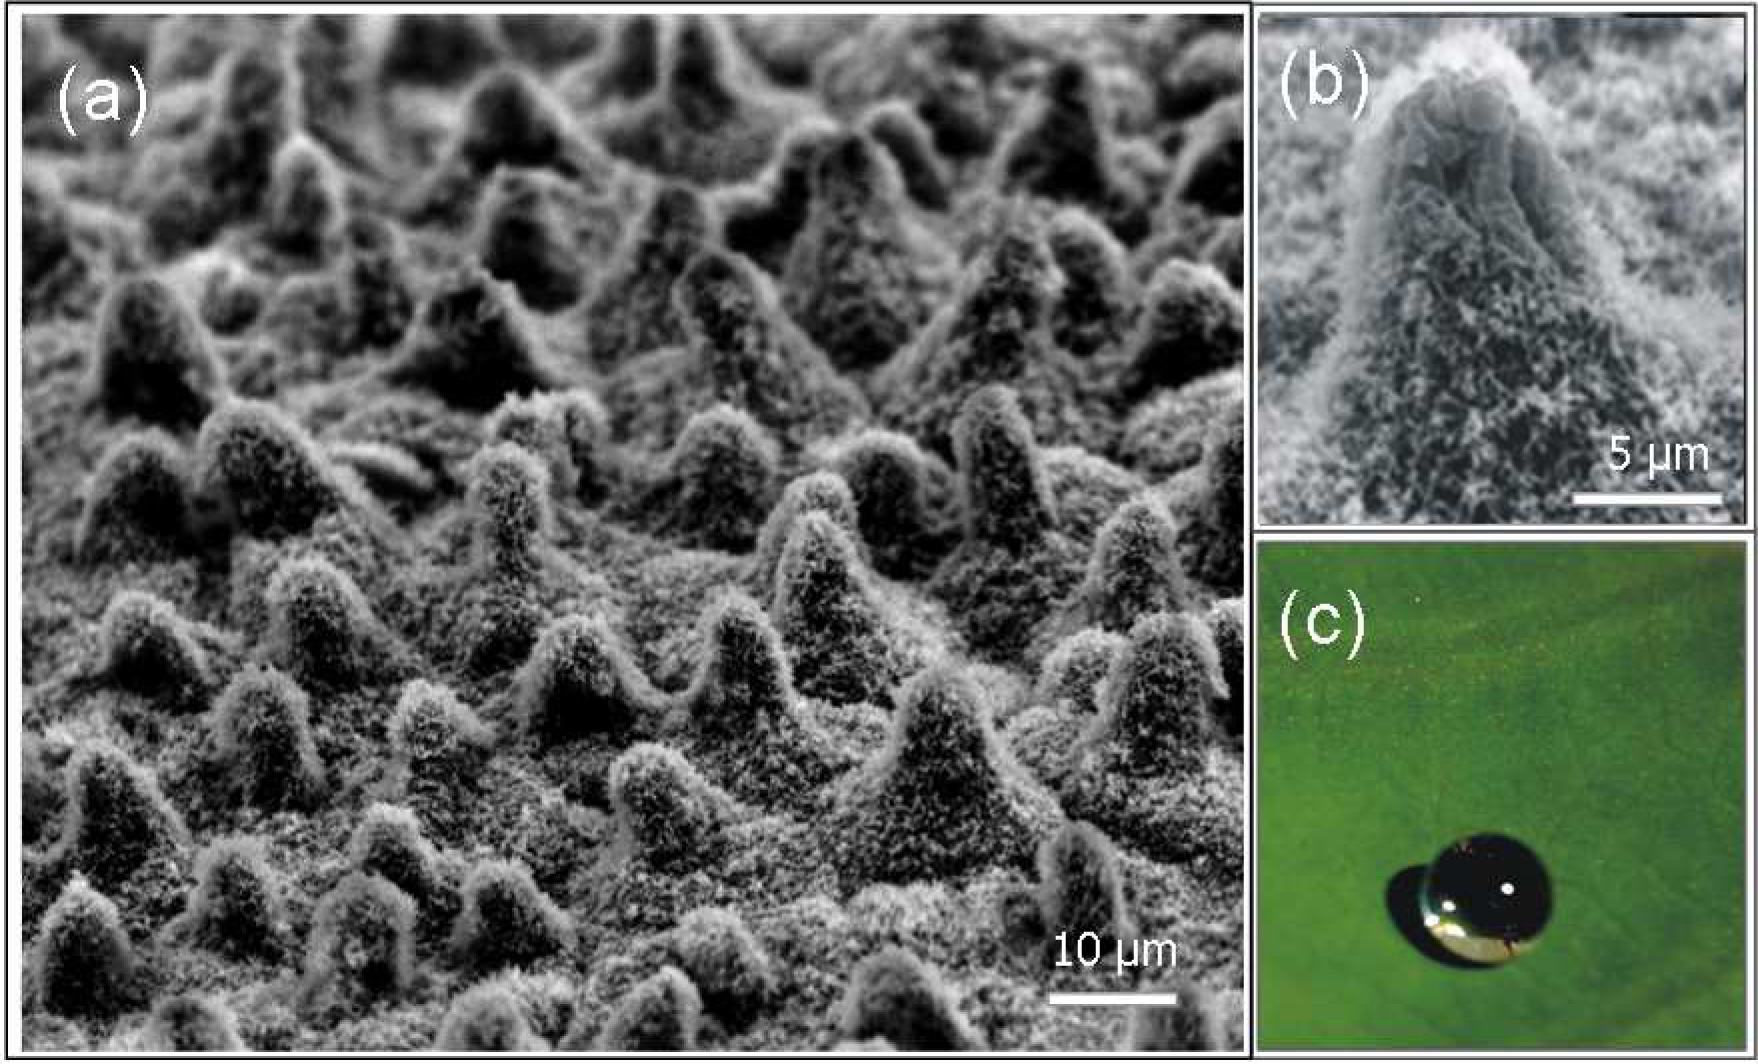
\includegraphics[width=0.6\linewidth]{chapter_1/lotus}
	\caption{(a) Scanning electron microscopy (SEM) image showing the structure of lotus leaf, (b) higher order of magnification on the single protuberance forming the surface and (c) a water drop that due to the contact angle attain an almost spherical shape. Images from \citet{stratakis2009laser}}
	\label{fig:lotus}
\end{figure}

The interest reader could find other examples and broaden the above key aspect in \citet{bhushan2016biomimetics}, \citet{tropea2012nature}.

\subsection{Riblets and shark-skin surfaces}

We have seen that natural surface can be an inspiration to find strategies in solving many aerodynamics problems; in the following we will focus especially on the drag reduction.

Is known that the total drag contribution can be separated in different components, and the classical decomposition is between viscous drag (sometimes referred as skin friction) and pressure drag.

\begin{equation}
 \int_{A_{\sigma}}  [ \underbrace{\left( \frac{p}{\rho} \mathbf{I} \right) \cdot  \mathbf{n}_{\sigma} }_\text{pressure drag}  +  \underbrace{ \left( \nu \nabla \mathbf{v} \right) \cdot  \mathbf{n}_{\sigma}}_\text{viscous drag} ] \; dA,
 \label{eq:force}
\end{equation}

In \eqref{eq:force} $A_{\sigma}$ is the solid interface of some body where a no slip condition is applied, and $ \mathbf{n}_{\sigma}$ is its outward normal.
This section will talk about the existing ways to reduce the viscous part of the drag since historically has attracted more interest and/or make more progress.

In the following we will refer as the wall shear stress in the turbulent case as:

\begin{equation}
\tau = \left( \left( \mu + \mu_t \right)  \nabla \mathbf{\overline{v}} \right) \cdot  \mathbf{n}_{\sigma} = \left( \mu + \mu_t \right) \derp{\overline{u}}{y}
\end{equation}

where $\mu_t$ is the turbulent viscosity and $\overline{u}$ is the average velocity stream-wise component; in the laminar case obviously the definition rest the same with the appropriate corrections (there is no turbulent viscosity and no notion of average velocity).

Most of the industrial application involves turbulent flow; obviously there is a lot of research that aim to reduce the skin-friction in this regime.
Table 6.3.1 in the book of \citet{mclean2012understanding} make a wide list of technique already been proposed on the problem.

As the same author pinpoint, the most effective and, probably the most practicable concept are the riblets.
Riblets are alternating ridges aligned in the stream-wise flow direction and regularly arranged as the figure \ref{fig:riblets1} show.

These surfaces are capable of align the turbulent flow in the mean flow direction smoothing the fluctuation of the cross-flow in the viscous sublayer.
Reducing this fluctuations close to the surface the turbulent momentum transfer will also be reduced and so the shear stress, causing the reduction in skin-friction.

\begin{figure}[h]
	\centering
	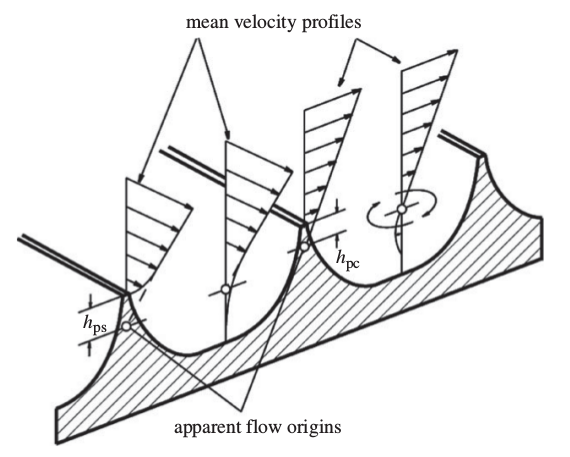
\includegraphics[width=0.7\linewidth]{chapter_1/riblets3}
	\caption{Schematics of the  \textit{protrusion height} concept. The mean velocity profiles for the stream-wise and cross-flow velocities are shown. In presence of a ridge is it possible to extrapolate the point of zero velocity from the velocity gradient outside the riblet; finding respectively, the \textit{stream-wise protrusion height} $h_{ps}$ and the \textit{cross-flow protrusion height} $h_{pc}$. Image from \citet{bechert1997experiments}}
	\label{fig:riblets1}
\end{figure}

The viscous drag reduction correlates well with the spacing between the ridges expressed in wall units $ s^+ $; the typical shape of the latter relation is depicted in figure \ref{fig:riblets_perf}, where the vertical axis show the drag reduction against the $ s^+ $.
This general shape of the curve, in which the skin friction decrease in certain range of spacing and then increase as the ridge spacing  increase, is caused by a competition between the capacity of riblets to obstruct lateral fluid flow and an increase in the penetration of high speed vorticies inside this manufactured rugosities.

\begin{figure}[h]
	\centering
	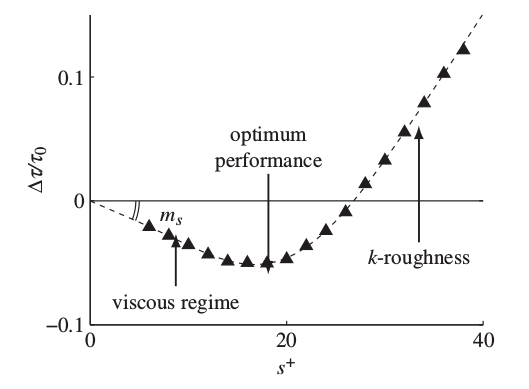
\includegraphics[width=0.5\linewidth]{chapter_1/riblets_performance}
	\caption{Example of drag reduction relation to the ridge spacing. The maximum performance is normally around $ s^+ = 15 $, the picture show also that when the riblet are really tight one another the laminar case is retrieved. On the contrary when the riblets are far away one other their performance is comparable to rough plate case. Image from \citet{jimenez2001turbulent} }
	\label{fig:riblets_perf}
\end{figure}

This last physical explanation of the riblets performances is presented in the schematics \ref{fig:riblets_schem}, where the gray areas show high skin-friction regions caused by the down-wash motion generated by the near-wall vortices.
Is it clear that when the riblets are too big the vortices can penetrate inside its groove, and actually increase the skin-friction due to larger area exposed to the local velocity.
On the contrary when the riblets are smaller, the high speed vortex "touches" only the tip of the ridges so only a small local area of the surface experience high-shear stresses.

\begin{figure}[h]
	\centering
	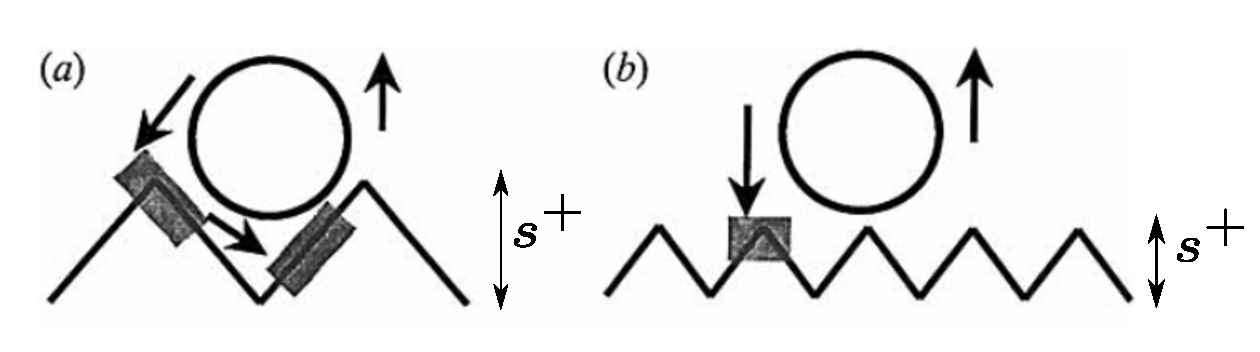
\includegraphics[width=0.7\linewidth]{chapter_1/riblets1}
	\caption{Two different size of riblets are shown when interacting with a sublayer vortex. In gray is it represented the areas where friction is important. Clearly when the size of two is comparable the surface experience a larger friction and the performance is lowered. Image from \citet{choi1993direct}}
	\label{fig:riblets_schem}
\end{figure}

The slope $m_s$ of the curve in figure \ref{fig:riblets_perf} can be predicted by linear stability theory or by means of empirical correlations \citet{garcia2011hydrodynamic}.

Computing the performance of such surfaces can be expensive since the most reliable quantitative theory for such problems are direct numerical simulations (DNS) or experiments.
There is only one other theory, besides the already cited expensive ones, that use the concept of \textit{protrusion height} showed in figure \ref{fig:riblets1} to correlates the shape of this protrusion to the drag reduction \citet{luchini1991resistance}.
The \textit{protrusion height} is defined as the vertical distance between the riblet top ridge and point of zero velocity extrapolated from the constant velocity gradient outside above the protrusions.
It seems that especially the difference of protrusion heights, computed from the stream-wise $h_{ps}$ and cross-flow flow $h_{pc}$ profile, correlates very well with the drag reduction, and the two quantities can be computed with a simple Stokes problem over the local geometry of the grooves.
The last results has been analyzed by \citet{segura2017permeable} that came out with an empirical law for the drag reduction, that relates the previous protrusion heights with the permeability expressed in wall units:

\begin{equation}
DR \approx 0.04\left( \sqrt{{K^+}_s} - \sqrt{{K^+}_c} \right),
\label{eq:max_dr}
\end{equation}

where ${K^+}_s$ and ${K^+}_c$ are the stream-wise and cross-flow permeability tensor components.
This law establish an instrument to estimate the drag reduction from a given geometry of the wall (the permeability tensor can be computed within the porous media homogenization approach as chapter \ref{ch:vans} will explain).

Another important characteristic of riblets performance is that they are robust in off-design conditions, such as in presence of yaw (misalignment between flow and riblets ridges) and tip ridges erosion \citet{garcia2011drag}.

But still, besides some very specific application such as sailing competitions (the hulls of the USA challengers in the America’s Cup 1987 and 2010), the massive utilization of this technology is still in question.
Producing such surfaces in a larger area, like the roof of a car or the wing of an airplane, can be an issue for a routine use; because riblets size need to be very little to be effective.

Riblets like surface has been observed in nature for many years, for example \citet{Martin2016riblets} found out that skimmer birds (Rynchops) have riblets like grooves in their beak, since they fly with it under the water surface to catch fishes.
However, as already introduced, the most clear example of such natural surfaces are shark skin.
In his review \citet{dean2010shark} present the status of the shape optimization that has been done on the riblets trying to mimic the typical sawtooth shape seen in shark skin, showing that improvements of such geometries over the classical ones has yet to be proven.
Shape optimization on riblets geometry has been studied, the findings show that just a few $\%$ can be improved on the base line geometry \citet{bechert1997experiments}.

There is in fact some controversial result in literature stating that surfaces with actual shark skin replica can indeed increase drag.
\citet{boomsma2016direct} perform some simulations on actual shark skin denticles using the immersed boundary method; the authors find that in some configuration the actual drag increase up to $40\%$, but even though their numbers are probably too large (it is know that the immersed boundary method can generate some errors especially in computing forces at high Reynolds number), this can be a clue that the shark skin does not work with the same mechanism as riblets.

Experiments on such geometries are available in literature \citet{bechert1997natural}.
The authors of the previous work have built a synthetic surface made by artificial shark denticles posed on top of springs and measure that even with the introduction of  surface elasticity the actual drag was increasing.
However the authors pinpoints that the actual shark flow regime is not steady as the experiments that he performed, and they speculate that the excellent swimming performance of the shark came from the separation control that flexible denticles can increase in the periodic oscillating flow that the swimming generate.

Experiment using DPIV on a NACA profile covered with actual skin samples of "Isurus oxyrinchus" mako shark, has been performed by \citet{lang2014SharkControl}, confirming that the flexibility of sharks denticles act as a passive flow control in order to avoid early separation.
In fact the experiments proves that for angles of attack larger than $15^{\circ}$ the flow reversal is almost completely avoided.
The same author introduce the importance in the different geometries of the denticles in various part of the body that obviously experience disparate flow condition,
\citet{motta2012Shark} perform a detailed collection of flexibility and scale measurement of different shark species that can be valuable for future studies.

Swimming experiment from \citet{Oeffner785}, who used a flat plate covered with real shark skin, also confirm the previous flow control mechanism and also make some conjectures about possible thrust enhancing controlled by the same movable scales that can move away the leading edge vortex.

Also \citet{itoh2006turbulent} shows that movable rugosities can outperform riblets, the authors in fact measure the drag reduction of a seal fur (that present fibrous movable surface) against a riblet surface in an experimental channel; its results are show in figure \ref{fig:seal}.

\begin{figure}[h]
\centering
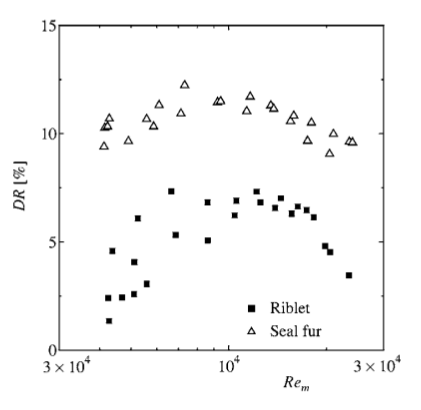
\includegraphics[width=0.5\linewidth]{chapter_1/seal}
\caption{Performance comparison between a riblet surface against a seal fur. The drag reduction has been computed as: $DR \% = \dfrac{ \Delta \tau}{\tau_{0}} \%$ Image from \citet{itoh2006turbulent}.}
\label{fig:seal}
\end{figure}


Compliant surfaces can in fact move accordingly to the surface pressure gradients along the boundary layer and so respond to the pressure fluctuation over the surface itself.
This mechanism is already know to be beneficial in delaying the transition to turbulence and many authors have presented theoretical and experimental evidence on the effectiveness of this solution \citet{carpenter1990status}, \citet{bushnell1977effect}.

In conclusion we have seen that in order to reduce turbulent skin-friction drag, riblets and natural surfaces uses various mechanism such as: sublayer vortices interaction, compliance and separation control.
Such solution have proven to be effective in some cases but they are related mostly in reducing the viscous component of the total drag.
In the next section we will introduce another class of solution that try to act instead mostly on the pressure component.


\subsection{Permeable surfaces}

\subsection{Bluff bodies}

%Permeable surface has been proposed to exploit even further the mechanism explained above using riblets.
There is some experimental evidence that in laminar cases the generation of some \textit{slip velocity}, at the interface between the permeable surface with the fluid, can decrease the friction drag \citet{beavers1967boundary}.
However in the turbulent case it seems that the instabilities developing at the interface can cause an increase in drag up to $40\%$ \citet{jimenez2001turbulent}, \citet{breugem2006influence}; this instabilities mechanism will be further explained in the section \ref{sec:stability}.
Is important to pinpoint that the permeable surface cited in the above references were all rigid.

The pressure contribution to the resistance is usually the most significant one in bluff bodies applications, and even in highly streamlined body it is around $10\%$ of the total drag.
Researchers have tried to find a way to modify the pressure distribution around a bluff body to reduce the associated resistance, and also dump the force oscillation on the body (drag and/or lift).

The pressure drag on a bluff body depends mostly on the difference between the low pressure on the rear part of the body, where there is usually a separated flow region, and the high pressure in the forward part.
This idea is sketched in figure \ref{fig:pressure_dist} where two different pressure distribution are shown; the black one represent the classical solid body, and the green one is the one with a porous layer at the back of the body.

\begin{figure}[h]
	\centering
	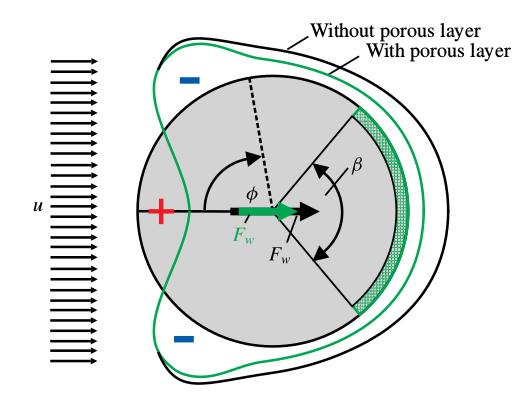
\includegraphics[width=0.4\linewidth]{chapter_1/pressure_dist}
	\caption{Diagram showing an example of angular pressure distribution around a cylinder for viscous flow. The black line is the case of a solid body, the green one is the modified pressure in presence of a porous layer at the rear part. Image from \citet{klausmann2017drag}}
	\label{fig:pressure_dist}
\end{figure}

The favorable increase in the back pressure is due to the low speed laminar flow in the porous media that is ejected in the back region where the separation take place.
Even in very high speed turbulent flow the fluid inside permeable surface exhibit a very high energy loss due to the strong dissipation that the medium provide, resulting in a low speed flow ejected downstream of the body.

The permeable interface, producing a slip velocity, can modify the boundary layer that develops above it and with that produce less shear and vorticity; and can also modify the stability characteristics of the flow.
The instability around a cylinder is due to the shear layer that forms in the top part of the body when the flow start to decelerate.
This shear layer exhibit a Kelvin–Helmholtz type instability that develop in the classical Von-Karman wake.

This two hypothetical mechanisms has been tested by numerical simulation by multiple authors: \citet{bruneau2004passive}, \citet{bruneau2008numerical}, \citet{bhattacharyya2011reduction}, \citet{naito2012numerical}, \citet{mimeau2017passive}.
All these works study the flow around some classical two dimensional bluff bodies (cylinder, square cylinder, Ahmed body section, 3D hemisphere) with the add of a porous layer.

These works show some very promising result on multiple quantities, like: decrease of enstropy, lower oscillations in lift signal, drag reduction, regularization of the wake and lower pressure gradients; even if the porous medium is always rigid in their case.
An example is shown in figure \ref{fig:porous_cylinder} where the flow field downstream to a square cylinder is computed in a turbulent case; the picture show how the porous layer strongly regularize the wake.

\begin{figure}[h]
	\centering
	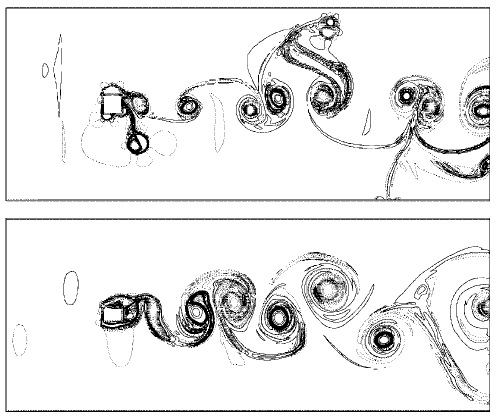
\includegraphics[width=0.7\linewidth]{chapter_1/cylinder_porous}
	\caption{Square cylinder vorticity contour for $Re=30000$. Top: solid case. Bottom: porous case with layer extension $h=10\% D$.}
	\label{fig:porous_cylinder}
\end{figure}


It seems from the previous works that the porous medium parameters, like the medium resistance or its vertical extension, have important effects on the results.
They seems to agree (at least qualitatively) that increasing the porous medium extension over a certain limit is not beneficial, and they also show that the resistance of the medium should not be excessive in order to be effective (high/medium porosity are the best).

In all these work we observe a reduced pressure drop between the front and the rear of the body, reduced drag, delays in the vortex shedding in the laminar case and regularization on both the frequency and amplitude of shredded vorticies oscillations.

These early work show very optimistic numbers but they should be taken with some care; only few cases are three-dimensional, and they all use a modeling approach for the porous medium based on a simplified version of the VANS (volume average Navier-Stokes equations, see section \ref{sec:vans}) without performing any validation of the method, and sometimes they use the equations outside their field of validity (there is some discussion in the scientific community in using such methods for highly turbulent flows).

The lack of validation reflect the fact that reliable experiment of such porous coatings are almost non existent in literature.
They also do not agree on the methods used to compute the forces \citet{caltagirone1994interaction}?? SHOW HERE THE GOOD METHOD ? MAYBE IN THE VANS SECTION...


\citet{favier2009passive} use a different numerical method that includes the dynamic of a moving porous medium made of fibers at the back of a cylinder.
Their results in a laminar flow case agree with the results on the stabilization of the wake and show some more realistic values of drag reduction, about $15\%$.
The difficulties in this model is in the medium dynamic, since it introduce many mechanical parameters that are not easy to identify for natural surfaces.

A similar model to the previous one has been used by \citet{venkataraman2012numerical}; the authors applied a movable porous coating in the top part of NACA airfoil.
In this case the synchronization between the oscillations of the structures and the natural frequency of the fluid is responsible for the pressure distribution modification.
They have shown the robustness of this solution in a wide range of angle of attack, in the best case they have found some lift enchantment and regularization and a drag reduction has been measured to be on the order of $10\%$.

Later on \citet{rosti2017pelskin} works on a similar configuration with only one movable flap on the low pressure side of airfoil; the results both numerical and experimental qualitatively agree (on the flow mechanism) with the results in the complete porous case.


WHEN IT WILL BE PUBLISHED SHOW SOME RESULTS ON THE 3D SPHERE USING HOMOGENIZATION \citet{zampogna2017new}

The are very few experiment in literature on this porous coatings, but they all seems to show less promising numbers when  dealing with drag reduction.

For example \citet{heenan1998passive} perform an experiment in which he take a backward facing step with a porous insert in the re-circulation region.
His measurement show a $13\%$ decrease of the peak of pressure at the wall and a relocation of the detachment point further downstream.
Also depending on the length of the porous insert a maximum of $9\%$ of drag reduction was also observed.
The effect of adding a porous surface in this case was to limit the pressure fluctuations that causes the re-circulation bubble unsteadiness.

Later \citet{klausmann2017drag} study a 3D cylinder with a porous insert in the back; the authors use a wind tunnel testing with pressure measurements around the body and particle image velocimetry (PIV) flow capture.
Their results confirms that the porous layer on the leeward side increase of pressure in that zone, causing the reduction of drag.
The drag reduction measured to be around $10\%$ over various Reynolds number in the fully developed turbulence range, but it can be more sensible to the geometrical parameters of the medium as the position and its size.
At our knowledge this is the first example of actual measurements of flow quantities using PIV, that can later be used to perform some validation on different numerical models.

Some other experimental data can be found in the case of flow over aquatic canopies \citet{zhang2011exchange}, \citet{segalini2011experimental}, \citet{hamed2017impact}, even though the published data is limited and the problem in this case has also a free surface that increase the difficulty of the problem and limits the possible use as validation.

From this section the main physical mechanism that tied to permeable surfaces has been introduced but the different approaches in literature seems to be discordant in the predicted values of some fundamental items such as the forces.
Is it clear that the scientific community need much more experimental data in order to develop new and improved numerical and theoretical models for such permeable coatings.

\subsection{Canopy flow}

Another important class of flow over poroelastic carpets are the \textit{canopy flow} as known in literature; they are flow over flexible slender structure as threes or aquatic vegetations.
The importance of winds over plants is very important in a large variety of fields, like: the transport of substances as $CO_2$ and nutrients or preventing agricultural damage (wind-throw of crop fields); also the above examples show some dynamic similarities even with urban canopies \citet{ghisalberti2009obstructed}.

It is known that the turbulent boundary layer profile over a canopy differ substantially from the rough wall one, figure \ref{fig:spectra}.
The vegetation resistance (drag) cause the creation of an inflection point in the mean velocity profile that lead to a mixing layer type of instability near the vegetation top.
In the work of \citet{finnigan2000turbulence} the author focused on the turbulent feature of the flow field in presence of vegetation.
He show that the vegetation can heavily modify the turbulence spectra as a results of the interface instabilities and the coherent structures above it.
As the two bottom pictures in figure \ref{fig:spectra} show, the spectrum in the case of canopy flow present a larger peak in the frequency of the mixing layer instability, a steeper slope in the energy cascade part due to the larger dissipation inside the permeable layer and possible high frequency peaks associated to the swinging of the pants that can emit or absorb small scales vorticies.
 
\begin{figure}[h]
	\centering
	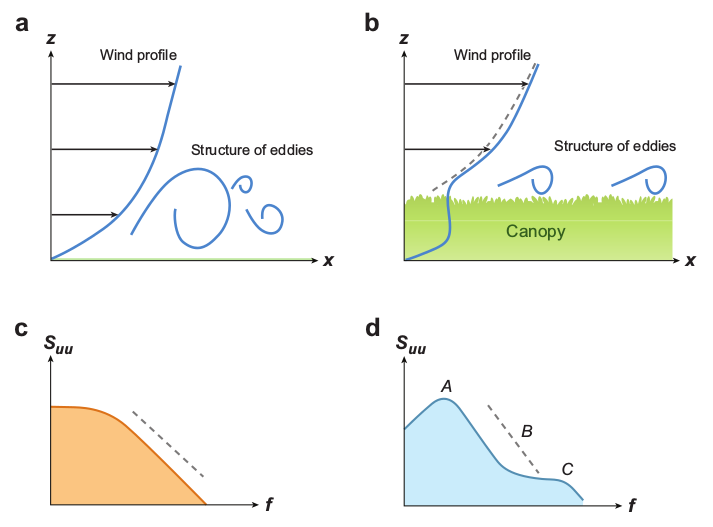
\includegraphics[width=0.7\linewidth]{chapter_1/spectra}
	\caption{bla bla \citet{de2008effects}}
		\label{fig:spectra}
	\end{figure}

So is it clear that the dynamic of the permeable substrate made by vegetation is extremely important and should always take into account to fully generalize the physics in such problems involving moving canopies.
As shown in \citet{nepf2012flow} especially for aquatic plants the movements of the plants can be important and so the interface can be largely modified.

In order to discriminate the different behavior of the fibrous structure we need to introduce some important non dimensional parameters used in fluid structure interaction problems:
$$ m^* = \rho_{\beta} / \rho_{\sigma}, \quad C_Y= \rho_{\beta} U^2 s^3 / E, \quad s = L/\ell $$
The first one is the mass ratio, the second is called Cauchy number and the last one is the slenderness of the structure.
The mass ratio $m*$ is a measure of the added mass effects caused by the solid inertia, but this effects are usually negligible in case of fibrous permeable media.
The Cauchy number $C_Y$ define the static deformation of a solid caused by the fluid flow ($E$ is the modulus of elasticity of the solid material), at Cauchy numbers over the unity important deformation are expected.
This number is extremely important since it control a phenomena called \textit{reconfiguration} that leads to drag reduction \citet{gosselin2011drag}, \citet{alvarado2017nature}.
The reconfiguration is the capability of the structure to adopt a new shape when forced by a flow, it can become more streamlined and/or reduce its exposed frontal area with the aim to reduce the total drag.
When dealing with this phenomena we should take together the frontal area $A$ and the drag coefficient $C_D$ to avoid misinterpretation of the drag reduction; in figure \ref{fig:cycd} this ratio has been represented for different natural structures against the Cauchy number and is it clear that for a $C_Y>1$ we have a drastic drag reduction.

\begin{figure}[h]
	\centering
	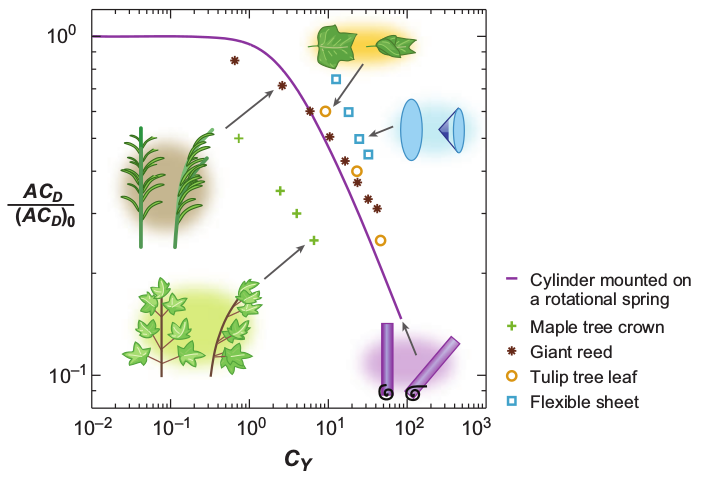
\includegraphics[width=0.7\linewidth]{chapter_1/cy_cd}
	\caption{The effect of the Cauchy number $C_Y$ on the drag reduction are presented in the figure. The drag reduction has been represented has the ration between the frontal area $A$ and the drag coefficient $C_D$ at static condition (subscript $0$) and the dynamic condition. Image from \citet{de2008effects}}
	\label{fig:cycd}
\end{figure}

The overall reconfiguration of the permeable medium can lead to pressure recovery and a wake regularization applied to a bluff body, as the experiments by \citet{gosselin2011drag} show.

Another important non dimensional number is the \textit{reduced velocity} and it can be derived form the previous ones as:
$$ U_R = \sqrt{C_Y s / m^*},$$
this number is used dealing with vortex induced vibration of slender structure, if it is in the order of unity it means that some dynamical coupling between is expected such as resonance or lock-in.

Canopies can help to prevent separation in presence of adverse pressure gradients, \citet{belcher2012wind} show an analysis of the flow over an hill covered with canopies using either numerical and experimental data; the authors show how the permeable layer can present a recirculation region inside the canopy in the decreasing slope side of the hill, so moving the separation from the flow over the hill to the internal structure of the canopy.
In this sense when we look at the "global" hill (ground and canopy layer) the reversed flow typical of this geometry is not present.

Is important to pinpoint that the above results are restricted to fibrous or slender structure, and they cannot be extrapolated in general for all different porous structure ans shapes, even though similar mechanism are expected.

In the case of canopy flow is very difficult to compare results because most of the authors use very different models in a lot of regimes of velocities and using flexible structure with very different shapes.
Even if much more experiments are available \citet{segalini2011experimental}, \citet{segalini2013scaling}, \citet{maza2013coupled}, \citet{barsu2016drag}, \citet{alvarado2017nature}, there is no quantitatively mathematical model established for the fluid and structure equations and most of them rely on empirical correlations that fit the data of each different case.


\section{Models for flows through porous surfaces}

In this section we want to state clearly what is the problem that we are trying to solve and which characteristic are the difficult one.
In order to be as clear as possible we have taken the simplest example to define the problem; the flow over a wall that include multiple flexible filaments. 
This is probably the simplest geometrical configuration to think about but it still has all the characteristic and difficulties of more interesting configuration, such as a bluff body with a poroelastic layer.

\begin{figure}[h]
	\centering
	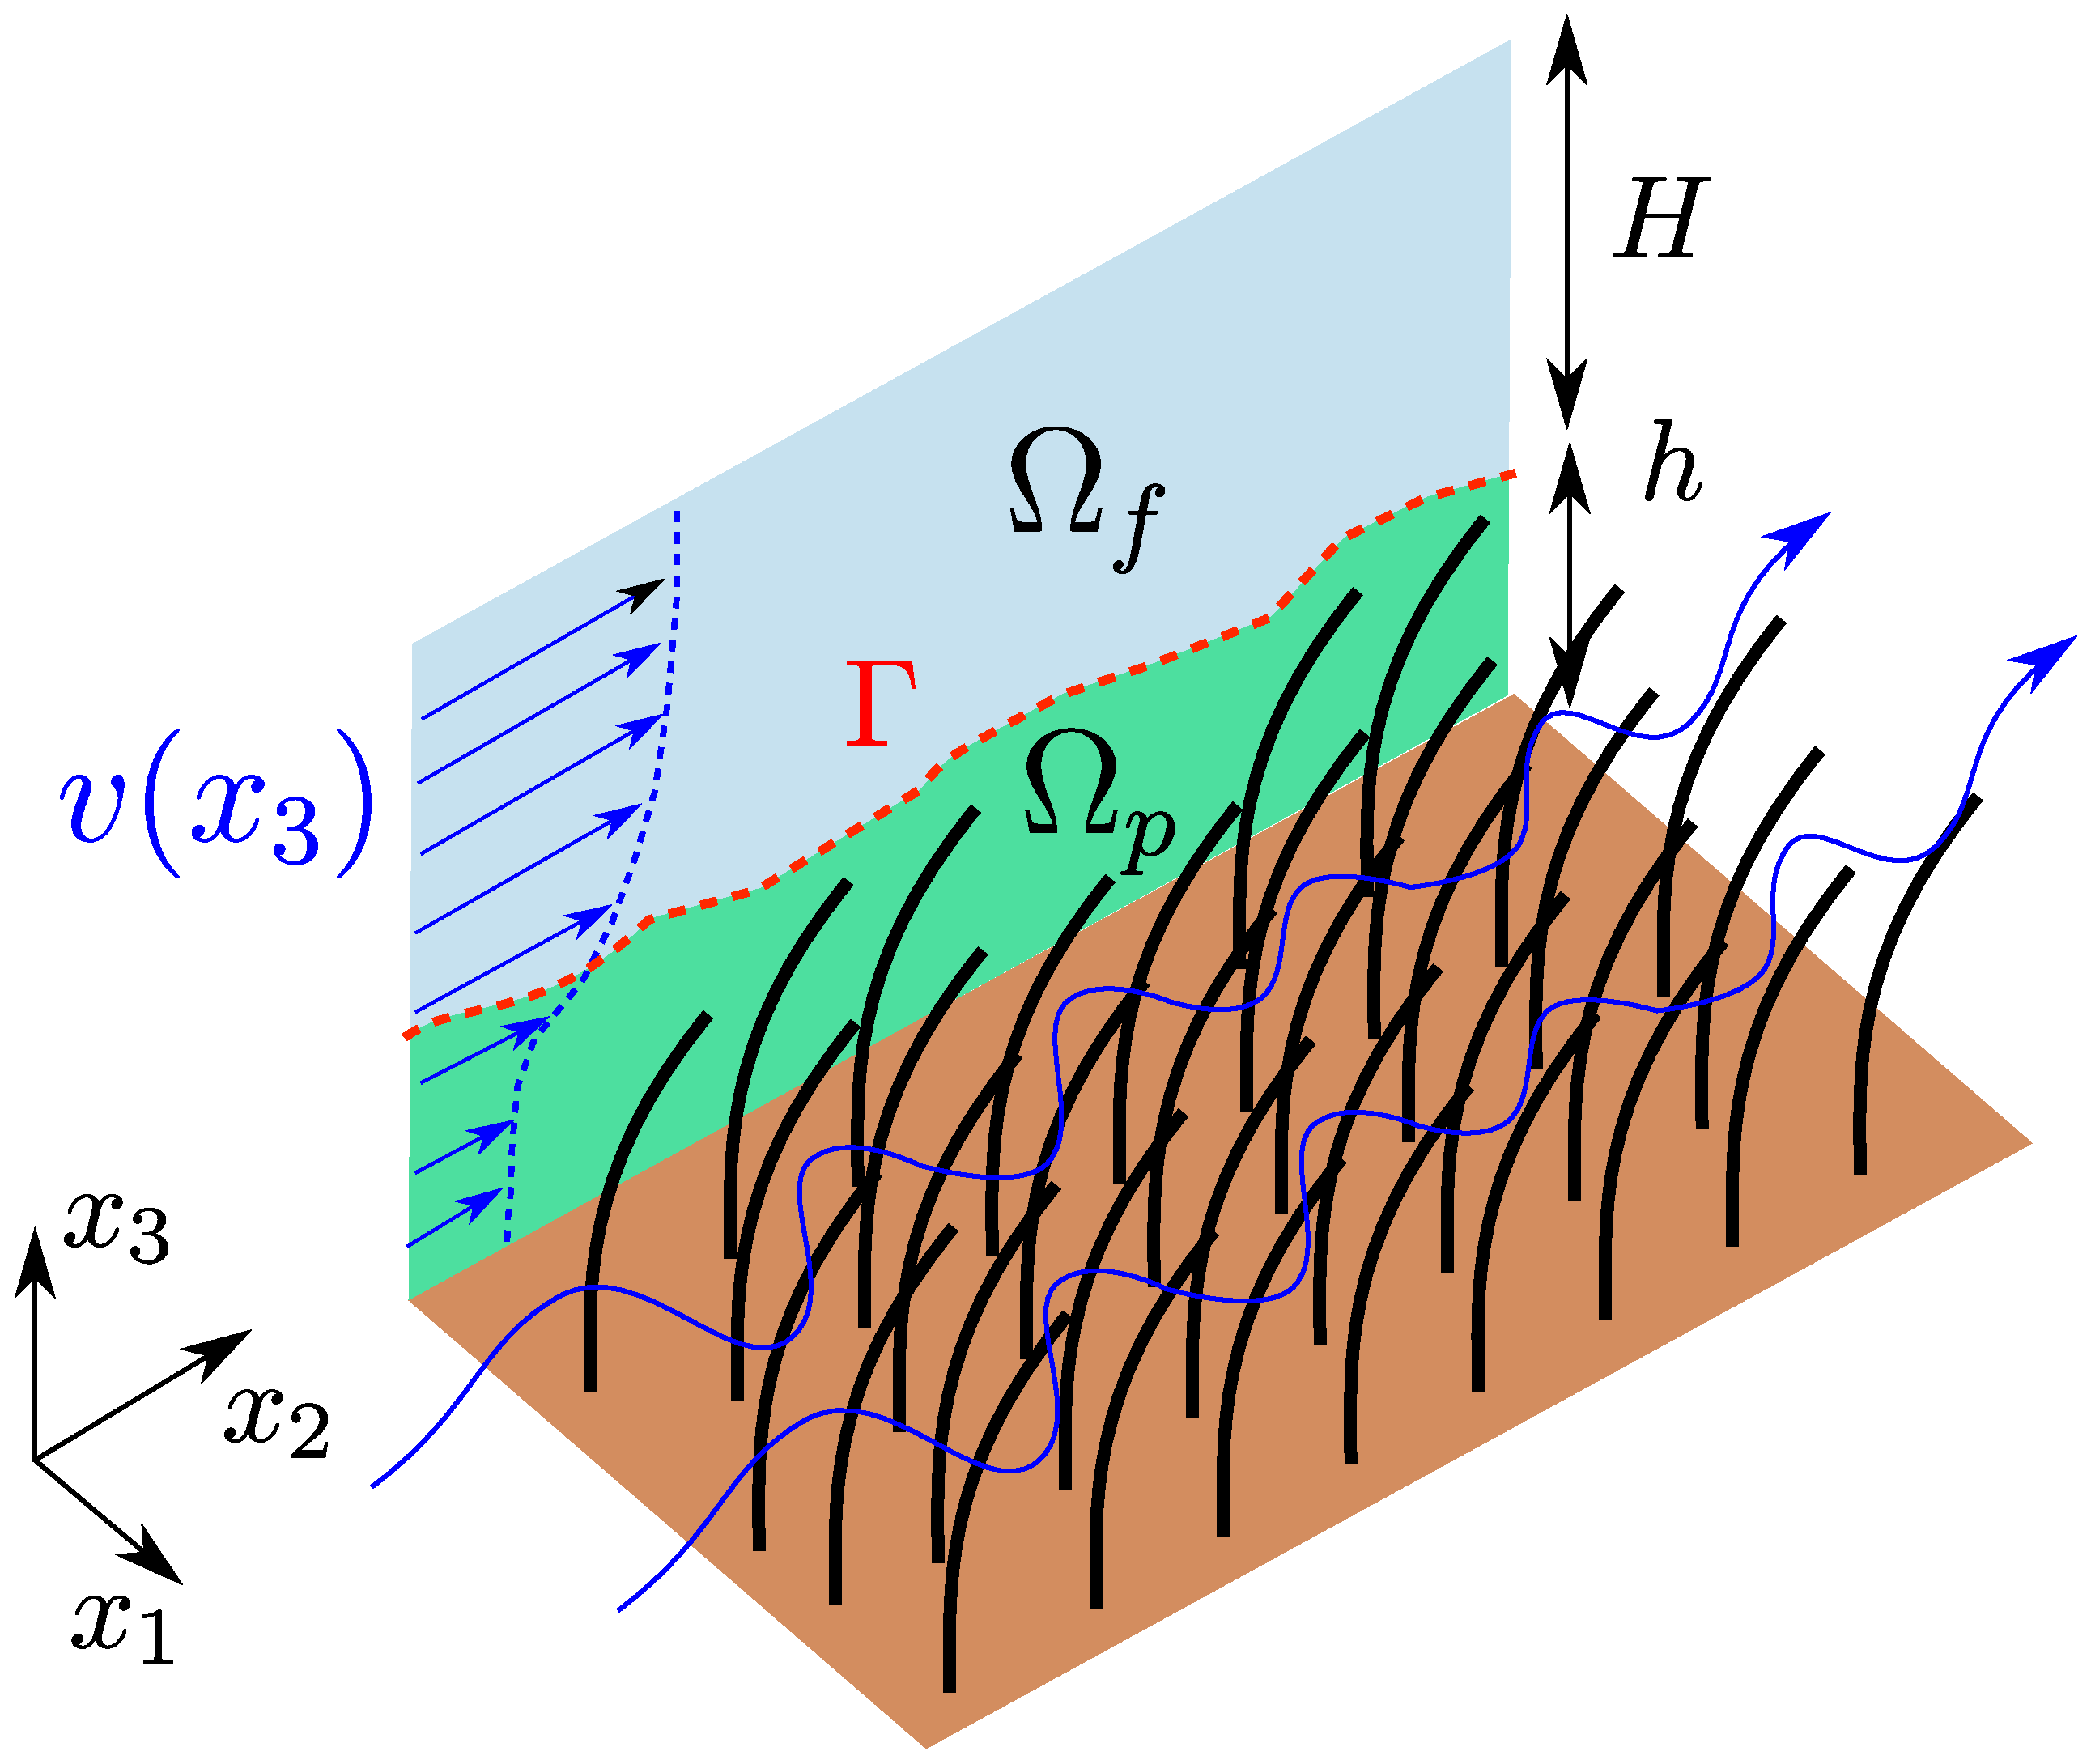
\includegraphics[width=0.7\linewidth]{chapter_1/problem_schema}
	\caption{Sketch of the fully developed flow over a poroelastic surface made of multiple filaments.}
	\label{fig:schema_problem}
\end{figure}

The figure \ref{fig:schema_problem} show a graphical schema of such flow; the fluid main direction is aligned with the $x_2$ axis and the projection of the stream-wise component is shown in the plane $x_2 - x_3$.
Such flow can bend the filaments and, of course, pass through their ensemble.
The hypothetical surface that envelop all the filaments ends ($\Gamma$), defines the limit between the flow without obstacle ($\Omega_{NS}$) and the one inside the poroelastic medium ($\Omega_{P}$), their projection are shown in the  $x_2 - x_3$ plane.

In order to computationally solve this problem there are some key points:
\begin{itemize}
	\item Length scales: the flow is very rich of multiple scales vorticies. The flow can have Kelvin–Helmholtz instabilities on the interface (that has the size of $h$) but they can even penetrate inside the medium and brake up to very small scales. In order to resolve this complex dynamic one should have a very fine mesh (very computational expensive) or came up with a model (like in turbulence).
	Also the turbulence dynamic can be a problematic; the hypothesis that turbulence can exist in porous media is still at debate in the community.
	Deal with such small scale dynamic and find a model for at least the interface part (in which the Kelvin–Helmholtz vorticies forms and brake up) is not an easy task.
	
	\item Compliance (Fluid structure interaction): if the filaments are flexible they bent and swing due to the fluid force that act on them.
	We have to take into account a mechanical solid model for the filaments such as the Bernoulli beam, and compute the energy that the swing of the filaments will re-inject inside the fluid flow.
	This two-way coupling could be also really computational expensive in presence of a large number of filament structures, and also if the the filaments are really flexible one should in principle take into account the possibility of contact and repulsion between the fibers.
	If the medium has a much more complicated shape (like the scales in the butterfly) one probably cannot use simplified models sor the solid dynamic and so use a general FEA discretization on the solid that is even more expensive.
	Another approach consist of consider a general model for the medium, for example treat it like a porous medium that can have elastic properties.
	Such models mimic the dynamic of the solid and in theory are more adapted to porous media that are fully connected, in principle they are very computational convenient but their mathematical description can e difficult and one should agree on the idea of losing information inside the medium.
	
	\item Anisotropy: the problem should be capable of treat permeable surfaces that have different response when stressed in different directions. For example the geometrical disposition and/or the mechanical properties of the medium can be non homogeneous, so the medium will be more permeable in one direction and so have a preferential flow path.
\end{itemize}

Examples of full resolved fluid-structural problem in which either the flow and the filaments structure has been resolved directly are very few in literature.
\citet{marjoribanks2017does} performs large eddy simulation over a bed with $300$ filaments; but he use a very simple drag model for the fibers mechanics and use a one way coupling between the solid and the fluid, so he resolve the fluid, pass the forces on the solid, compute the new solid position and directly go to the next time-step without re-iterating.
Even with a simple coupling and solid dynamics the flow show some insight in the fibers dynamic, but again the lack of validation makes the results questionable.

\citet{dupont2010modelling} previously made a similar model introducing a two way coupling for the fluid-structure interaction problem, this time they validate their code with video recording of a similar experiment and the frequency measurements of the Kelvin–Helmholtz instabilities at the interface agrees very well.
The authors so not give quantitative information of the computational configuration but mention a very important high performance computing center in the acknowledgment which made us suppose that the computational power involved were substantial.

Show other examples that solve directly the full coupled problem are in \citet{pinelli2017pelskin} \citet{favier2017pelskin}, \citet{revell2017pelskin} but in this case the number of filaments is small and so they can be though more as singular filaments that a really poroelastic medium.

There is of course another way to treat the problem state ìt above that does not use \textit{brute force}.

Due to the computationally expensiveness on solving the problem directly the scientific community has came out in time with different approaches that treat the porous domain with a generalized model that do not resolve the fine scale inside and between the filaments but instead express them as a function of the length scales present in the fluid domain $\Omega_{NS}$.

The key point in such methods are:
\begin{itemize}
	\item They divide the overall domain in two different parts: the fluid domain $\Omega_{NS}$ and the porous domain $\Omega_{P}$
	\item Two different fluid models are solved in the two domains, in $\Omega_{NS}$ the Naver-Stokes equations for incompressible fluids are the classical choice, and in the porous part there are a number of different models that usually neglect the temporal derivative and the convective part in the latter equations but adds other source terms in order to take into account the presence of the solid inclusion that form the porous medium
	\item The two domains are coupled together with an interface boundary condition or a special equation treatments for this transition region
	\item A model for the dynamic of the solid porous part should also be chosen
\end{itemize}

Also the interface treatment and the solid model can be tied to the choice of the porous fluid model.
The source term introduced in $\Omega_{P}$ depends on the theory in which we develop our porous media model, in the next two section we will talk about the two main branches existing in literature.

\subsection{Isotropic drag models}
\label{sec:canopy_eq}

In the case of flow through vegetation (canopy flows) it is common to use a simpler isotropic drag model for parametrize the resistance of the canopy.
So the drag is usually function of the depth (the distance from the interface in the wall normal direction) and it is supposed to be isotropic; this hypothesis can be correct in case of dense vegetation when the flow cannot generate almost any wake inside the canopy, but it is certainly wrong in the wall normal direction since for a flow purely vertical the resistance of the medium should be smaller.
However since this models are mostly applied in channel problems where the mean flow is mostly stream-wise the resistance in the vertical direction can be approximated in this manner, but in application where the transpiration of the interface is important (wake control of bluff body) the isotropic drag model is certainty not convenient.

The drag resistance is included in the incompressible Navier-Stokes equations as a sink of momentum as in equation \ref{eq:mom_cd}.

\begin{equation}
\derp{\vb}{t} + \vb \cdot \nabla \vb = -\frac{1}{\rho_{\beta}} \nabla \pb + \nub \nabla^2 -C_D a |\vb| \vb, 
\label{eq:mom_cd}
\end{equation}

The sink term is quadratic in the velocity but there is some evidence that the reconfiguration phenomena can change this relationship taking into account the drag reduction \citet{gosselin2011drag}, \citet{alvarado2017nature}.

The sink term includes also the parameter $a$ that is the frontal area per unit volume of the vegetation and even if it has the dimension of a length this parameter is an expression of the porosity of the medium.

For our point of view this approach lack of strong mathematical formalism, from which one should be able to derive all the additional terms of the equations; as a consequence, this method heavily rely on empirical relations.
One other problem is that the isotropic hypothesis rule out the possibility to model the anisotropic nature of most of the surfaces in which we are interested (as equation \ref{eq:max_dr} suggest the difference in the permeability in different directions can be important for the drag reduction).

But in the field of vegetations a lot of authors have successfully used this approach in various domain, for example \citet{maza2013coupled}, \citet{maza2015tsunami} use it to study wave attenuation, \citet{ghisalberti2004limited}, \citet{battiato2014single} develop a simple model for the 2D mean flow over a canopy.


\subsection{Homogenization models}

The above section introduce the idea to look at the problem as it was composed by two different domains; here in this section we want to introduce the most used approach to derive the equations that are valid in the porous domain in an \textit{averaged} sense.
The fundamental idea is to construct a micro-scale model, either for the fluid as for the solid, and then derive the macro-scale equations using some averaging operator over the micro-scale.

The two most known homogenization methods are the \textit{Volume Averaging} method \citet{whitaker2013method}, and the \textit{Multiple Scales} method \citet{mei2010homogenization}; they can be more broadly classified as perturbations methods. 
The key differences and the main results retrieved within this approaches will be presented in the following.


\subsubsection{Volume Averaging}
\label{sec:vans}

The method of Volume Averaging has been developed to threat transport equation in porous media applications; in this case the presence of two different length scales is obvious as in figure \ref{fig:porsystem}.
	
	\begin{figure}[h]
		\centering
		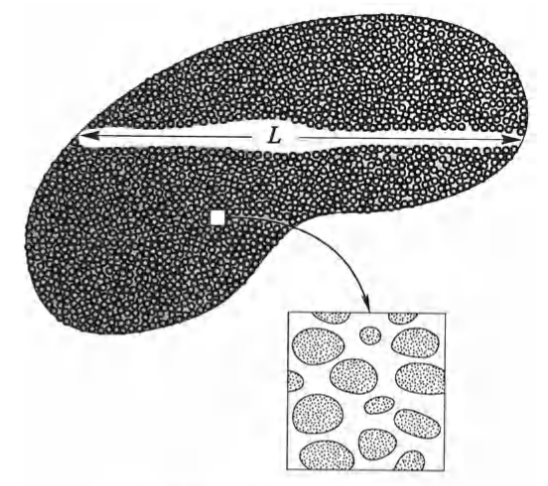
\includegraphics[width=0.7\linewidth]{chapter_1/por_system}
		\caption{dfdfsfd}
		\label{fig:porsystem}
	\end{figure}

The core idea of the methods is that we can firstly define an average operator as \eqref{eq:avg_intrinsic_intro}, in this case the variable $\psi$ can be any vector or scalar variable in the system of equations that we want to homogenize, for Navier-Stokes it will be the velocity and the pressure.

\begin{equation}
\meani{\psi} = \dfrac{1}{\volb} \int_{V} \psi \, d \, V,
\label{eq:avg_intrinsic_intro}
\end{equation}

The average operator has the purpose to "scale up" the equation, in fact the second crucial step of the method is to decompose the variables as proposed by \citet{gray1975derivation}:

\begin{equation}
\psi =   \underbrace{ \meani{\psi} }_\text{O($L$)}  +  \underbrace{\tilde{\psi} }_\text{O($\ell$)},
\label{eq:vans_decomp}
\end{equation}

The \eqref{eq:vans_decomp} show how each variable can be decomposed in an averaged part that contains only spatial variation at the macro-scale $L$ and a \textit{fluctuation} part that contains only the micro-scale $\ell$ spatial variations.

The decomposition can be injected in the transport equations that we want to homogenize, and new transport equations that includes only variables of order O($L$) can be retrieved.
Since this is the method chosen to solve our problem, all the technical details will be detailed explained in the chapter \ref{ch:vans}.

The most famous application of the method is the Stokes flow inside a rigid porous medium as the one in figure \ref{fig:porsystem}, the $\beta$ subscript indicate the liquid phase:
\begin{equation}
0 = -\dfrac{1}{\rho_{\beta}} \nabla \pb +\nub \nabla^2 \vb
\label{eq:stokes}
\end{equation} 

Here is important to note that the equation \eqref{eq:stokes} is valid only in the liquid phase and to solve it we have to consider all the solid phase as rigid boundaries, with the difficulties that came to define the complex structure of the solid inclusion.
Applying the Averaging Method we can derive an homogeneous version of the \eqref{eq:stokes} that is valid in the all the porous domain that include the two different phases, the solid and the liquid one; the famous Darcy equation \eqref{eq:darcyeq} \citet{whitaker1986flow}.

\begin{equation}
\vbmi = -\dfrac{\mathbf{K} \varepsilon}{\mub} \nabla \pbmi
\label{eq:darcyeq}
\end{equation} 

In the Darcy equation is possible to recognize two additional quantities that arise from the averaging procedure, the fist one is a scalar called porosity $\varepsilon$ and represent the ratio of the liquid phase present in a reference volume of the medium.
The second one is the tensor $\mathbf{K}$ called permeability, it express the resistance of the porous medium that affect the flow in its travel.
The term $\mathbf{K}$ play the same role as $C_D a$ in the isotropic drag model; but the main difference is that the permeability tensor can be computed directly from the geometry of the medium (see chapter \ref{ch:vans}) so it does not rely on empirical relations.
Also the tensorial nature of this terms permits us to model porous inclusion that are anisotropic in nature.

Applications of the theory include: fluid inertial terms \citet{whitaker1996forchheimer}, porous media with small deformations \citet{whitaker1986flow2}, and high deformations \citet{hussong2011continuum}, turbulence \citet{soulaine2014}, \citet{breugem2006influence}, interface between a permeable medium and a free flow \citet{beavers1967boundary}, multiphase systems \citet{whitaker1973transport}, heat transfer \citet{carbonell1984heat}.

Here we do not want to go into details of the derivation of equation for our specific problem but we want just to be clear about the differences of this method to the isotropic drag model of the previous section.
One of the greatest differences is the robustness that came from a mathematical formalism instead of an approach rely heavily on experimental closure terms.

\subsubsection{Multiple Scales}

The multiple scale method is similar to the previous one; and it has also been applied to similar problems in the context of porous media applications.

In this method we start with the assumption of scale separation between the two length scales, $\ell$ micro-scale and $L$ macro-scale; the scale separation factor can be defined as $\epsilon = \ell/L \ll 1$.
Using the same examples as before we want to show the how to compute the homogenized version of the Stokes equation for fluid flow through a porous media.
We introduce the micro-scale and the macro-scale coordinates of the problem defined respectively as:
$$
 X_i = \dfrac{\tilde{x_i}}{L}, \quad   x_i = \dfrac{\tilde{x_i}}{\ell},
$$
where $x_i$ are the original coordinate of the problem.
Using the above separation factor is possible to expand the variables of the problem (pressure and velocity) into orders (like a Taylor expansion) indicated with the number as superscript:
$$
\psi(X_i, x_i) = \psi^{(0)}(X_i, x_i)  +\epsilon \psi^{(1)}(X_i, x_i) +\epsilon^2 \psi^{(2)}(X_i, x_i) +O(\epsilon^3),
$$
injecting this decompositions inside the equation \eqref{eq:stokes} is it possible to derive a set of system of equations for each order of the expansion.
It can be shown that analyzing each equation in the set we can retrieve the homogenized equation:

\begin{equation}
{v_i}^{(0)} = -K_{ij} \dfrac{\partial p^{(0)}}{\partial X_i}
\label{eq:darcy_ms}
\end{equation} 

In which either the pressure and the velocity fields appear only at the order zero, and the equation depends only on the macro-scale length.

We find the same permeability tensor $\mathbf{K}$ as before, and its definition is the same.
So it is clear that for this example problem we find as results the same set of homogenized equation; it only change the starting hypotheses of the method and the mathematical development to compute them.

A full analysis of the dualism of the two approaches can be found in the work by \citet{davit2013homogenization}.

The multiple scale also has been used to study: inertia effects \citet{mei1991effect}, \citet{skjetne1999new}, coupling between a free fluid and a porous media \citet{mikelic2000interface}, porous media with small deformations \citet{auriault1977etude}, heat conduction in composites \citet{auriault1983effective}, rigid and moving permeable layers \citet{zampogna2016fluid}, \citet{ugis}, \citet{zampogna2017pelskin}.

Is also worth mention another homogenization based method called mixture theory, based on similar approach is it possible to retrieve the same equation as the previous two methods \citet{rajagopal2007hierarchy}.


\section{Stability of flow over permeable surfaces}
\label{sec:stability}

Flows through submerged aquatic plants exhibit large scale vortices at the top of the vegetation,
advecting along the flow direction and causing a periodic waving of the plants, referred to as
monami (if the fluid is air) and honami (in case of water) \citet{inoue1955studies}, \citet{ackerman1993reduced}.
The effect of the onset of the monami is depicted in figure \ref{fig:monai_evol}.


\begin{figure}[h]
	\centering
	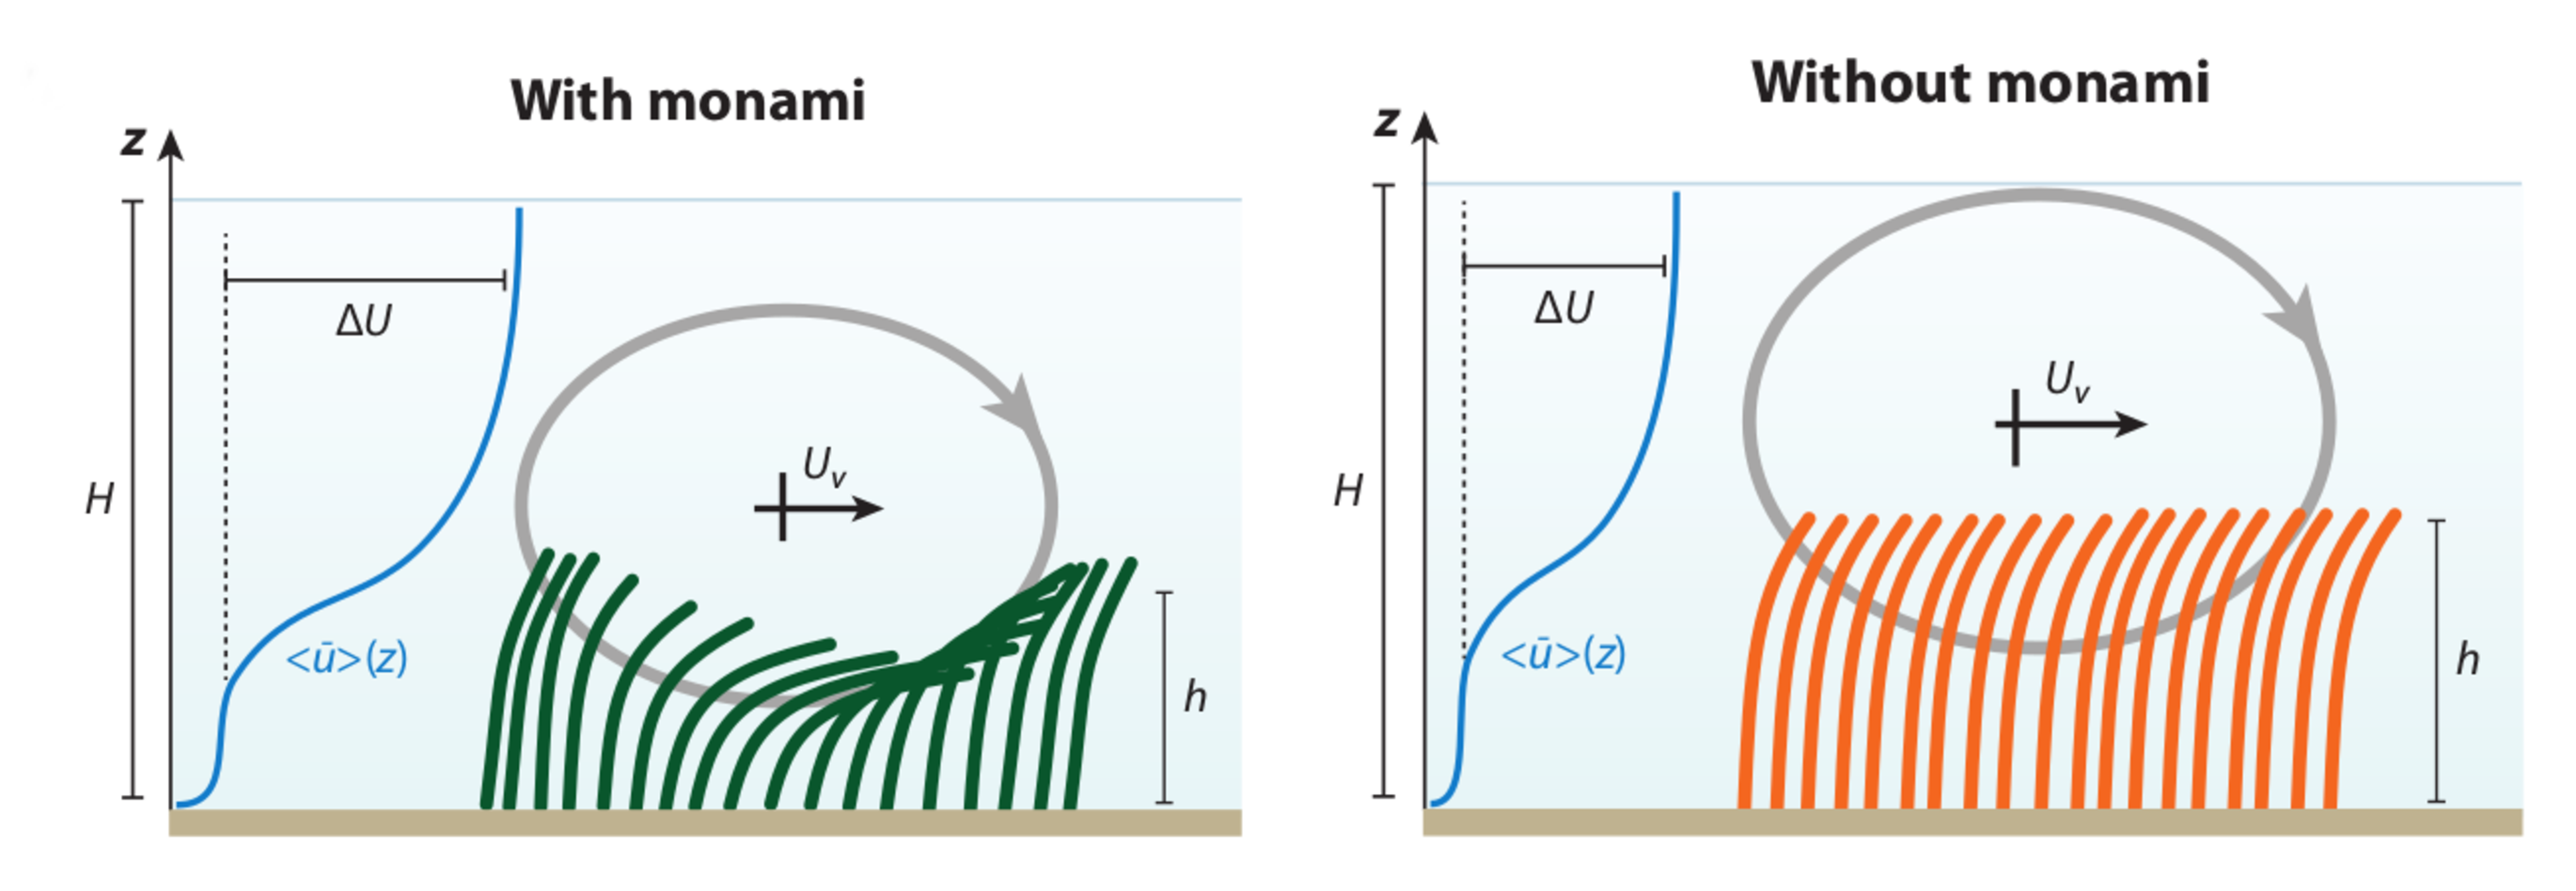
\includegraphics[width=1\linewidth]{chapter_1/monami}
	\caption{When the drag of the canopy is high enough it generates canopy-scale vortices by Kelvin-Helmholtz instability. Left: These  vortices may interact with the flexible vegetation and generate a waving motion called monami. Right: When this interaction is too weak, the canopy will only bend. Image from \citet{nepf2012flow}}
	\label{fig:monami}
\end{figure}

Vortices arise from the nonlinear amplification of a Kelvin-Helmholtz instability mode, related to the presence of an inflection point in the base flow profile \citet{asaeda2005morphological}; the profile itself is inflectional because the fluid is slowed down by the drag exerted by the canopy, whose modeling has recently been addressed \citet{py2004mixing} \citet{singh2016linear}  \citet{zampogna2016instability}, \citet{tilton2008linear}.
The correct prediction of the onset and characteristics of the Kelvin-Helmholtz instability is important for assessing the effects of turbulence \citet{finnigan2000turbulence}, \citet{jimenez2001turbulent} in particular to:
\begin{itemize}
	\item understand how the vertical exchange of momentum occurs \citet{ikeda1996three}
	\item clarify how the transport of $\text{CO}_2$ , dissolved nutrients or sediments takes place between the
	obstructed vegetation flow and the free overflow motion \citet{gambi1990flume}, \citet{eckman1987role}, \citet{grizzle1996hydrodynamically}
	\item assess the changes in the morphology of the vegetation in inland or coastal wetlands in
	response to continuous periodic forcing \citet{asaeda2005morphological} \citet{patil2010characteristics}
\end{itemize}

On of the possible approach to study how and when these instability develops is the linear instability analysis; in the following we will briefly introduce the key assumption and simplifications of the method over other possible choices, and in the next section some results of applications in the context of permeable surfaces will be presented.


\subsection{Stability theory generalities}

Stability theory in general covers the modeling of transition of fluids systems towards non stables states and at least turbulence.
In its most basic form the theory gives us a fast and robust method to compute the frequency and grow rate of the unstable modes, if there is any, in the base flow.

The linear stability relies on the decomposition of the flow variables $\mathbf{q}$ into a steady state part $\overline{\mathbf{q}}$ called base flow, and an unsteady part $\widetilde{\mathbf{q}}$:

$$ \mathbf{q} (\mathbf{x},t)= \overline{\mathbf{q}} (\mathbf{x}) + \epsilon \widetilde{\mathbf{q}} (\mathbf{x},t) $$

Than the unsteady part is simplified by the hypothesis to have a general wave form:
$$  \widetilde{\mathbf{q}} =  \widehat{\mathbf{q}} e^{i\Theta} $$

where the $\widehat{\mathbf{q}}$ is the amplitude and the $\Theta$ is the phase of the perturbation.
The choice made to determine the time and space dependence of either the phase function and the base flow determine a certain hierarchy inside the stability theories; the table below \ref{fig:table} show the main choice made in the literature and the theory that derive from it:

\begin{figure}[h]
	\centering
	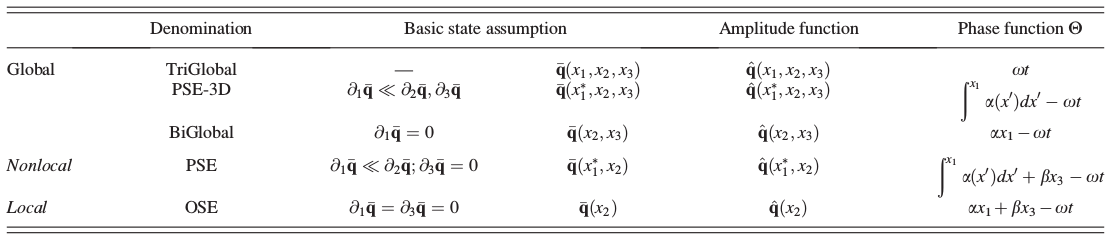
\includegraphics[width=1\linewidth]{chapter_1/table}
	\caption{Classification of modal linear stability theories. Table reported from \citet{juniper2014modal}}
	\label{fig:table}
\end{figure}
 
In our case we have limits our study in the linear stability theory (LST), that is a local approach based on mode decomposition.
In the LST we made the hypothesis that the base flow depends only on the wall normal spatial coordinate and the phase function take into account the periodicity of the flow in stramwise and crofflow directions and in time.
The complete formulation is in the following equation:
 $$  \widetilde{\mathbf{q}}(\mathbf{x},t) =  \widehat{\mathbf{q}}(x_2) e^{i(\alpha x_1 + \beta x_3 - \omega t)}  $$ 
where:
\begin{itemize}
	\item $\alpha$ is the stream-wise wave-number
	\item $\beta$ is the cross-flow wave-number
	\item $\omega$ is the wave phase
\end{itemize}

Casting this form for the the pressure and velocity inside the Navier-Stokes equation and neglecting the second order terms we can reformulate the problem in a linear operator.
This operator describe the evolution of the perturbations, taking the $\alpha$ and $\beta$ wave-numbers as real numbers and $\omega$ as complex we study the stability of the perturbation in time evolution (\textit{temporal stability}).
So the operator takes the form of a generalized eigenvalue problem for the wave phase:
$$ A \widehat{\mathbf{q}}=  \omega B\widehat{\mathbf{q}} $$
the solution gives use the frequency (real part of the eigenvalues) and the grow rate (imaginary part) of the perturbation modes (eigenvectors) of the flow.

The above explanation is quite condensed but a lot of literature has been developed in these years, \citet{juniper2014modal}, \citet{criminale2003theory}, \citet{schmid2012stability}, the problem is also been extensively study in his computational aspect \citet{canuto1988spectral}.

\subsubsection{Monami/Honami and Kelvin-Helmholtz rolls}

We have already pinpoint that the above framework for the stability problem has been applied in some porous media flow (canopy) configurations, also including the vegetation movement.
Because of the flexibility of the vegetation, some theoretical studies have focused on the
modeling of the stems of the aquatic plants and their displacement in response to the forcing by the
water flow \citet{py2004mixing} \citet{patil2010characteristics} \citet{gosselin2009destabilising} \citet{py2006frequency}.

It has been studied by \citet{finnigan2000turbulence} that these large coherent structures control turbulence dynamics over the canopy. Movements of the latter, generate sweeps (and ejections) of fluids that generates counter-rotating stream-wise eddy evolving with the Kelvin-Helmholtz rolls.
This picture of the complex evolution of the rich vortex dynamics that take place over the canopy surface is shown in figure \ref{fig:monai_evol}.

\begin{figure}[h]
	\centering
	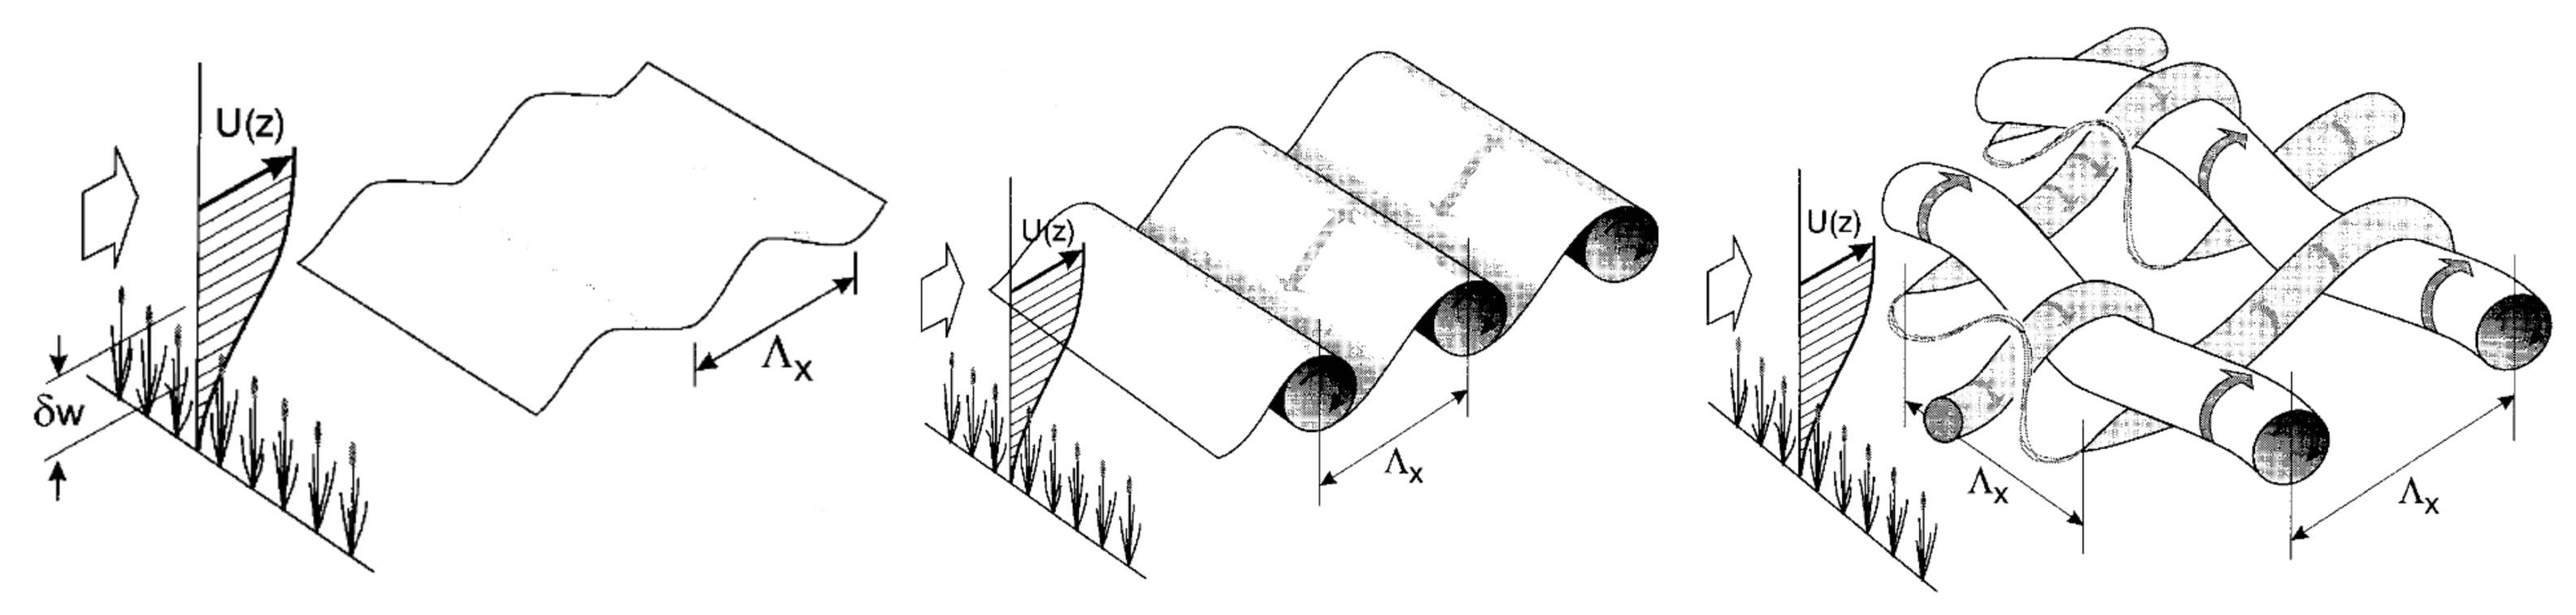
\includegraphics[width=1\linewidth]{chapter_1/finn}
	\caption{Left: first emergence of the Kelvin-Helmholtz instability, here the grow rate is proportional to the shear magnitude at the inflection point. Center: the instability evolve in rollers of consisting in high vorticity that are spaced with a similar wave-length $\Lambda_x$ as the previous stage.  Right:secondary instabilities in the rollers lead to their kinking and pairing, coherent structures shows up in the transverse and stream-wise dimensions. Image from \citet{finnigan2000turbulence}}
	\label{fig:monai_evol}
\end{figure}


However, Kelvin-Helmholtz vortices occur whether or not the plants bend and—to ascertain causes and effects to first order—it is acceptable to focus on the flow over and through a submerged array of rigid, cylindrical pillars.
This has been the basis of the approach by \citet{ghisalberti2002mixing} \citet{ghisalberti2004limited} \citet{ghisalberti2005mass} who have conducted a series of careful experiments; their results have often been
used by fluid dynamicists to put forth and test theoretical hypotheses to predict the frequency and
wavelength of the large scale vortical motion, for a variety of conditions.
The configuration studied consists of a regular grid of rigid pillars, orthogonal to the surface, of identical height h; in some
of the theoretical models proposed to analyze the stability of this system, the Rayleigh equation is
used throughout the water channel, with or without a drag term in correspondence of the canopy \citet{raupach1996coherent} \citet{py2004mixing} \citet{singh2016linear} \citet{zampogna2016instability} have recently demonstrated that the addition of a drag term through the vegetation reduces the amplification factor of the Kelvin-Helmholtz instability throughout the whole
range of wave-numbers and increases mildly the wavelength of the fastest growing mode.
In the chapter \ref{ch:stability} we will also study how the ??






\chapter{Volume Average Method}
\label{ch:vans}

\chapquote{Do not worry about your difficulties in mathematics; I can assure you that mine are still greater.}{Letter to junior high school student Barbara Wilson, \\ January 7, 1943}{Albert Einstein}

\section{Introduction}

As the previous chapter as introduced we are interested in the volume averaging method to scale up the fluid equations valid in the microscopic spaces of the porous medium and find a macroscopic description that is valid everywhere in the porous medium domain (not only in the fluid phase).
Theoretical aspect of the volume averaging method applied to fluid in porous media can be found in \citet{whitaker2013method}, \citet{whitaker1986flow}, \citet{whitaker1996forchheimer} CONTINUE THE LIST.
The following chapter describe the most important stages necessary to find the average version of equations \eqref{eq:NS}.

\section{Homogenization procedure}
The mathematical method of volume averaging is based on some fundamental stages that one should follow in order to retrieve the homogenized version of the equations.
We can resume the step as:
\begin{itemize}
\item Definition of the averaging operator
\item Use of theorems that permits to interchange the derivation and averaging operations
\item Decompose the fields in an "average plus perturbation" manner
\item Assume (based on the problem characteristics) some length-scales constraint that help to simplify the problem
\item Compute a final closed form of the homogenized equations
\end{itemize}

Such schema is graphically resumed in \citet{paez2017macroscopic} and \citet{davit2013homogenization}; a similar flowchart of the overall procedure is showed in figure \ref{fig:schema_vans_homo}.

\begin{figure}[h!]
	\centering
	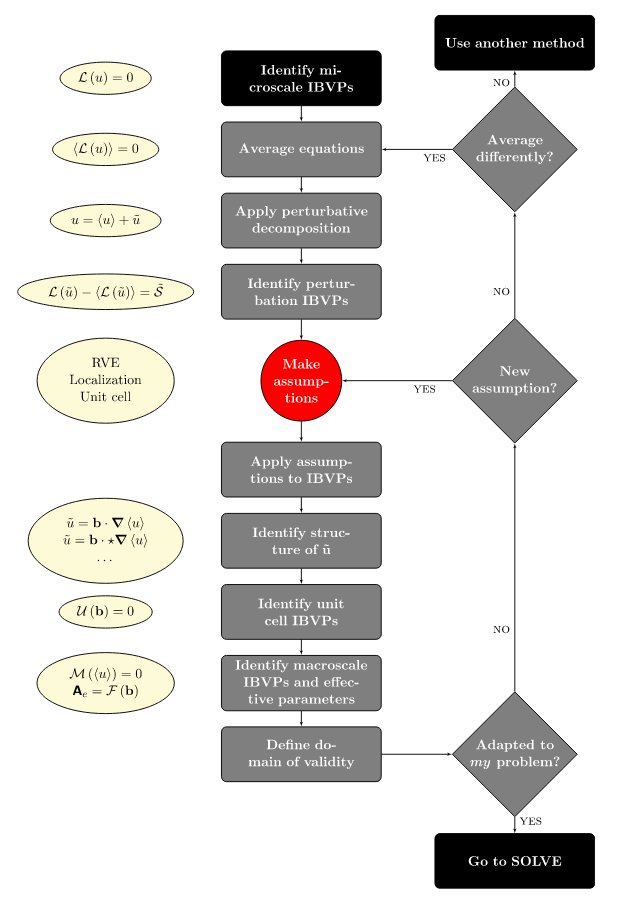
\includegraphics[width=0.8\linewidth]{chapter_2/figure/schema_vans_homo}
	\caption{Illustration of the volume average homogenization procedure. Image derived from \citet{davit2013homogenization}}
	\label{fig:schema_vans_homo}
\end{figure}

\section{Derivation of VANS equations for 3D incompressible fluids}
The dynamic of the fluid phase, indicated with the subscript $\beta$, is governed by the Navier-Stokes equation for incompressible Newtonian fluid; which in presence of a porous medium solid reads:

\begin{eqnarray}
	\begin{cases}
		\dfrac{\partial \vb}{\partial t} + \vb \cdot \nabla \vb = -\frac{1}{\rho_{\beta}} \nabla \pb + \nub \nabla^2  \vb  \\
		\nabla \cdot \ws = 0 \\
		\vb = \ws \qquad \text{at} \; A_{\beta\sigma}
	\end{cases}
\label{eq:NS}
\end{eqnarray}\\

where $\vb$, $\pb$, $\rho_{\beta}$ and $\nub$ stand, respectively, for  the velocity, the pressure, the density and the kinematic viscosity of the fluid, although  $\ws$ is velocity of the solid phase
The interface between the fluid and the solid is indicated as $A_{\beta\sigma}$, in which the no-slip condition for the velocity apply.
In the above equation we also need to specify initial condition in order to solve them, but the initial conditions do not take part in the homogenization procedure.

\subsection{Definition of the averaging operators}

\Red{show some support of averaging filters, talk a little bit on his hypothesis and meaning as a convolution product}

\Red{equation 1.6 in \citet{quintard1994transport4}}

Figure \ref{fig:rev} show a fibrous porous medium; all the quantities needed in order to develop our mathematical approach are also indicated.
The dotted lines in the figure are used to indicate the shape of the volume used in the average operators, $V|_{\mathbf{x}}$ indicate the overall volume with centroid $\mathbf{x}$ and $V_{\beta}|_{\mathbf{x}}$ indicate the volume occupied of the only fluid phase inside the same volume.
The coordinate $\mathbf{r} = \mathbf{x} +\mathbf{y}$ represent the centroid of a possible volume in which one can compute the average quantities.

\begin{figure}[h]
	\centering
	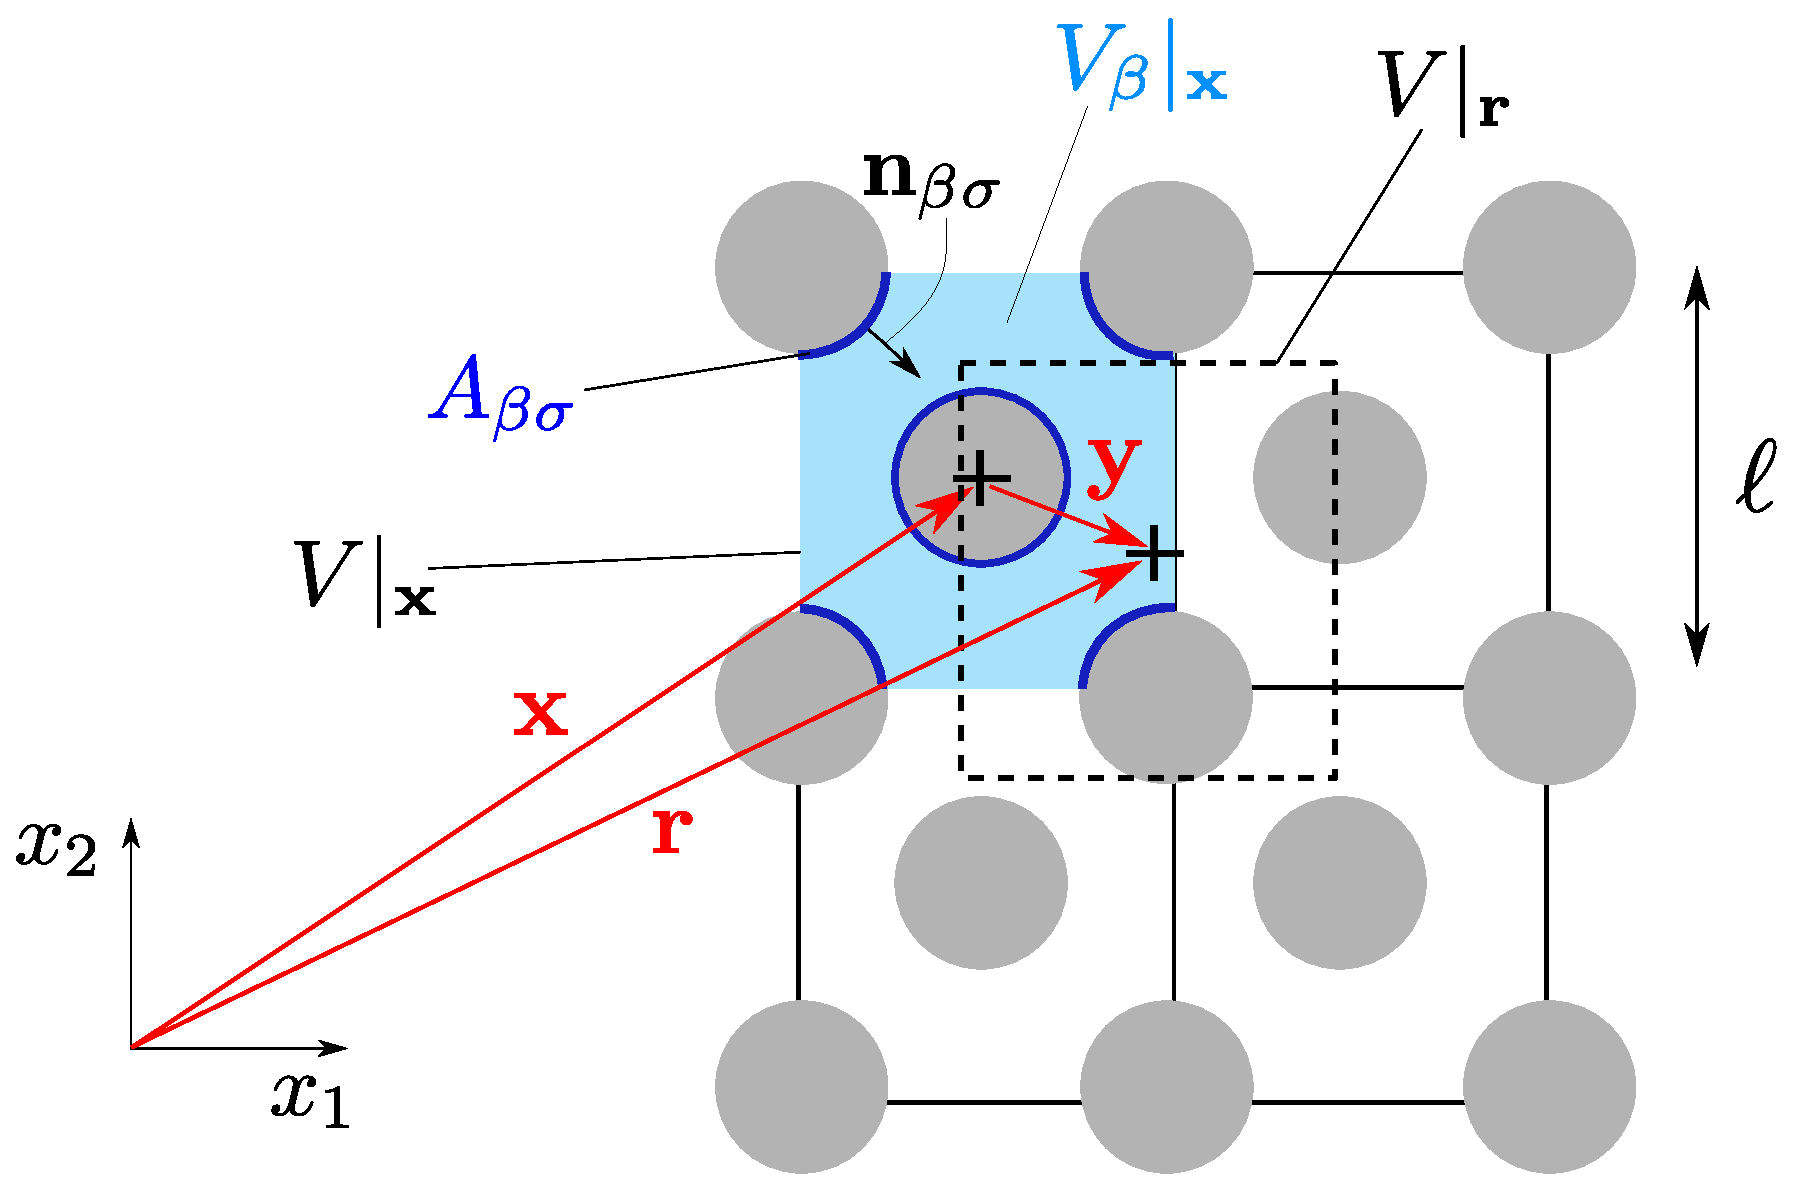
\includegraphics[width=0.7\linewidth]{chapter_2/figure/REV}
	\caption{A graphic representation of the averaging volume and interface in case of ordered porous media. In this example a fibrous  porous media in staggered arranged is depicted. In dotted lines the edges of the averaged volume are showed for two different centroid position ($\mathbf{x}$ and $\mathbf{r}$).}
	\label{fig:rev}
\end{figure}

Let $\psi_{\beta}$ be a an arbitrary order tensors (scalar, vector or second order tensor) defined on the volume $V$ with $x$ as centroid coordinates, we define two different spacing average operator.

The first one is called the \textit{intrinsic average} and is indicated as $\meani{.}$:
\begin{equation}
	\meani{\psi_{\beta}}|_{\mathbf{x}} = \dfrac{1}{\volb(\mathbf{x})} \int_{\volb(\mathbf{x})}  m(\mathbf{y}) \psi_{\beta}(\mathbf{x}+\mathbf{y}, t) d \, \volb,
	\label{eq:avg_intrinsic}
\end{equation}

where $m$ is a weight function defined on V and $\mathbf{y}$ is the relative position vector with respect to the centroid $\mathbf{x}$ of the averaging volume $\volb$.

The second one is the \textit{superficial average} indicated with $\means{}$:
\begin{equation}
	\means{\psi_{\beta}}|_{\mathbf{x}} = \dfrac{1}{V} \int_{\volb(\mathbf{x})} m(\mathbf{y}) \psi_{\beta}(\mathbf{x}+\mathbf{y}, t) d \, \volb,
	\label{eq:avg_superficial}
\end{equation}

In order to use a less heavy notation, the subscript $|_{\mathbf{x}}$ is dropped in the following procedure, but we keep in mind that the volume averaged quantities are explicitly dependent on the volume center.
Either averaging operators are defined as a volume integral over a certain volume of which size and shape should be chosen differently in each application; some more details on this choice are presented in the next paragraph.

Inside the average operators we can further use a weight function ($m$); that has the aim to guarantee smooth volume averaged fields.
However the choice of the shape of the filter depends on the porous media geometry, and its size is connected to the volume one.

For the sake of simplify the notation we will consider a filter $m$ to be constant and we drop it from the formulation of the average operators.
However any shape of the function $m$ can be used without formally change the final form of the averaged equation.

The porosity of a porous medium cell is defined as:

\begin{equation}
	\varepsilon = \dfrac{\volb}{V}
	\label{eq:porosity}
\end{equation}

which represent the ratio between the volume occupied by the fluid and the total elementary volume.

Using the above definition is possible to defy the relationship between the two averaging operators:

\begin{equation}
	\means{\psi_{\beta}} =  \varepsilon \meani{\psi_{\beta}}
	\label{eq:means_vs_meani}
\end{equation}

\subsection{Choice of shape and size of averaging volume and filter function}
\label{ch:filter}

The problem of choice of the filter has been extensively studied by the series of works \citet{quintard1994transport1}, \citet{quintard1994transport2}, \citet{quintard1994transport3}, \citet{quintard1994transport4}, \citet{quintard1994transport5} and more recently by \citet{davit2017technical}.

The authors above differentiate their results for ordered and disordered porous medium; and they show that for each cases a specific size of the filter/volume and their shape is needed.
Sometimes in the following text we refer to the volume in which the average procedure is applyed as REV, \textit{reference elementary volume}.
For disordered porous media a spherical volume is more appropriate, and the size of the REV ($\ell_V$) should satisfy the length scale constraint:
$$
\ell_{\beta} \ll \ell_v \ll L
$$

Instead for ordered porous media the volume shape most appropriate is a cubic one with the length of its side:
$$
O(\ell_{\beta}) = \ell_V \ll L
$$
that can be reinterpreted as the separation of scale parameter in multiple scale analysis $\epsilon = \dfrac{\ell_{\beta}}{L} \ll 1$.

\citet{ochoa1995momentum} confirm the same length-scales constraints even in case of an interface between a free fluid and a porous medium.


The size of it ($\ell_v$) should be chosen with the above specifications, the length scales constraint assure that the volume is large enough that periodic boundary condition can be applied in the exterior of the volume and, on the contrary it should be small enough to be sure to capture all the phenomena that take place at the micro-scale (scale $\ell_{\beta}$).
If the REV size is the correct one, increasing or decreasing its size, of a certain amount, should not change the averages quantities.

We have already said that the function can help to attenuate variation of the averaged fields due to geometrical fluctuations of the porous medium.
It has in fact the property of a low-pass filter for the perturbations fields.


The filter function plays an important role also in the development of the equation in fact (as showed later) in order to retrieve a local form of the VANS equations we have to be able to make the statements:
\begin{equation}
\means{\means{\psi_{\beta}}|_{\mathbf{r}}}|_{\mathbf{x}} = \means{\psi_{\beta}}|_{\mathbf{x}}
\label{eq:well_behaved}
\end{equation}

that is equivalent to say that the averaged fields contains small variations of at the micro-scale (inside the averaging volume $V$).
In order to satisfy this requirement certain filter choices can perform better than others, although also the size of the REV plays a role.
In appendix \ref{ch:appendix_a} at the end of this chapter we furter explain the details in the approximation needed in equation \ref{eq:well_behaved}.

For disordered porous medium the \textit{hat function} filter $m^{\sqcap}$ which has the form:
\begin{eqnarray}
	m^{\sqcap}(\mathbf{y}) 
	\begin{cases}
		\dfrac{1}{V} \qquad |\mathbf{y}| \leqslant r_0\\
		0 \qquad |\mathbf{y}|> r_0
	\end{cases}
\end{eqnarray}
can be used to produce smooth averaged fields.

Instead for ordered porous medium the literature show that triangle shaped functions called \textit{cellular filter}  $m^{\bigtriangleup}$  performs better:
\begin{eqnarray}
m^{\bigtriangleup}(\mathbf{y}) 
\begin{cases}
(\ell_{beta}/2 - |\mathbf{y}|) \qquad |\mathbf{y}| \leqslant r_0\\
0 \qquad |\mathbf{y}|> r_0
\end{cases}
\end{eqnarray}

Whichever is the choice on the $m$ shape, \citet{davit2017technical} has re-formulated recently the required hypothesis that a $m$ function should satisfy; without entry in the details of the study (that is beyond the aim of this paragraph) we present some of the most important hypothesis:
\begin{itemize}
	\item be normalized in as: $\int_{\volb}  m(\mathbf{y}) \; d\volb = 1$
	\item have compact support 
	\item $m*\psi_{\beta} \in C^{k}$ where $k$ represent the order of the closure \Red{explain better}, where the operator $*$ express a convolution
	\item 
\end{itemize}


As introduced above the average operation can be view as a convolution product between the filter function and the flow field quantities, \citet{marle1982macroscopic}:
$$
\means{\psi_{\beta}}|_{\mathbf{x}} = \dfrac{1}{V} \int_{\volb(\mathbf{x})} m(\mathbf{y}) \psi_{\beta}(\mathbf{x}+\mathbf{y}, t) d \, \volb = m*\psi_{\beta}
$$

Even though we have shown the importance of the filter function shape it should be clear that oder works in literature that had implicitly used the $m^{\sqcap}$ are not wrong even in case of periodic ordered porous media.
In fact if we assume that the field are well behaved (even without checking if the filter or the REV size are the good one) we assume that the equation \eqref{eq:well_behaved} olds and so some simplifications of the averaging operators are permitted.
This permits us to finally find a closed local form of the equation and possibly use the good filter a posteriori to smooth the fields.
However neglecting the use of the proper filter can translate in some problem interpretations of the averaged fields (as \citet{quintard1994transport1} show for the example case of hydrostatic pressure) so particular care should be used especially when making comparison to experiments.

In the following derivation of the equation we do not formally include any filter function inside the averaged operators in order to not make the notation heavier.
However in each passage in which hypothesis on the filter of on the REV sizes are needed to formally derive the equation it will be stated.

\subsection{Theorems involving derivatives of spatial averaged quantities}

In this paragraph we report some the theorems related to the volume averaging technique. The purpose to these theorems is to establish relations between volume averaged derivatives to derivatives of volume averaged quantities.

\begin{theorem}[Spatial averaging theorem]
Let $\psi_{\beta}$ be a scalar quantity defined in the fluid phase $\beta$, then:

	\begin{equation}
		\means{\nabla \psi_{\beta}} = \nabla \means{\psi_{\beta}} + \dfrac{1}{V} \int_{A_{\beta \sigma}} \psi_{\beta} \nbs   \;dA
			\label{th:spat_avg}
	\end{equation}
\end{theorem}

In the above $\means{\psi_{\beta}}$ is evaluated at $\mathbf{x}$ and the operator $\nabla$ express the differentiation operation in respect to $\mathbf{x}$ also.

\begin{corollary}[Vector form of \ref{th:spat_avg}]
	The vector form of the spatial averaging theorem is given by:
	
	\begin{equation}
	\means{\nabla \cdot \boldsymbol{\psi}_{\beta}} = \nabla \cdot \means{ \boldsymbol{\psi}_{\beta}} + \dfrac{1}{V} \int_{A_{\beta \sigma}}  \boldsymbol{\psi}_{\beta} \cdot \nbs \;dA
			\label{th:vec_spat_avg}
	\end{equation}
\end{corollary}

\begin{corollary}
	Applying the theorem \ref{th:spat_avg} to a constant field $\psi_{\beta} = 1$ we obtain:
	
	\begin{equation}
		\nabla \varepsilon = - \int_{A_{\sigma \beta}} \nbs d \, A,
	\end{equation}
\end{corollary}


\begin{theorem}[Reynolds transport theorem]
	Let $\psi_{\beta}$ be a scalar quantity defined in the fluid phase $\beta$, then:
	
	\begin{equation}
	\dfrac{\partial}{\partial t} \int_{\volb(t)} \psi_{\beta} \; dV =  \int_{\volb(t)} \dfrac{\partial \psi_{\beta}}{\partial t} \; dV + \int_{A_{\beta \sigma}(t)} \psi_{\beta} (\ws \cdot \mathbf{n}_{\beta \sigma} ) \;dA,
	\label{th:transport}
	\end{equation}
	
	where $\ws$ is the point velocity of the solid-fluid interface $A_{\beta \sigma}$.
\end{theorem}


\subsection{Averaged continuity equations}


We start by finding the averaged version of the continuity equation in \eqref{eq:NS}:

\begin{equation}
\means{\nabla \cdot \vb}   = 0
\label{eq:superf_avg_cont}
\end{equation}
Applying \ref{th:spat_avg} to the previous equation we get:

$$
\means{\nabla \cdot \vb} = \nabla \cdot \means{\vb} + \dfrac{1}{V} \int_{A_{\beta \sigma}}  \vb \cdot \nbs \;dA
$$
The boundary condition at the interface ($\ws = \vb$) imply that the integral above can be modified: 
$$=\nabla \cdot \means{\vb} + \dfrac{1}{V} \int_{A_{\beta \sigma}}  \ws \cdot \nbs \;dA$$
Now we rewrite the last term as if it was a result of the Reynolds transport theorem applied to a constant unitary scalar field:
$$=\nabla \cdot \means{\vb} + \derp{}{t} \dfrac{1}{V} \int_{\volb} \;dV  - \dfrac{1}{V} \int_{\volb} \derp{1}{t} \;dV $$
This results can be simplified; in fact the last integral is zero due to the time derivation of a constant field and the first term can be further developed, obtaining finally the averaged continuity equation \eqref{eq:avg_1}.

\begin{equation}
\nabla \cdot \means{\vb} + \derp{\varepsilon}{t} =0
\label{eq:avg_1}
\end{equation}


\subsection{Averaged momentum equations}

In this paragraph we compute the average version of the momentum equation in \eqref{eq:NS}:

\begin{equation}
\dfrac{\partial \vb}{\partial t} + \nabla \cdot (\vb\vb) = -\frac{1}{\rho_{\beta}} \nabla \pb + \nub \nabla^2  \vb
\label{eq:mom_1}
\end{equation}

In order to keep the procedure readable we show the development of each singular term separately in the same order as they appear in \eqref{eq:mom_1}.

\subsubsection{Temporal derivative term}

Using theorem \ref{th:transport} we can rewrite the first term of the equation as:

\begin{equation}
\means{\derp{\vb}{t}} = \derp{\means{\vb}}{t} -\dfrac{1}{V} \int_{A_{\beta \sigma}(t)} (\ws \cdot \nbs ) \vb \;dA,
\end{equation}

\subsubsection{Convective term}

Theorem \ref{th:vec_spat_avg} applied to the convective term gives us:

\begin{equation}
\means{\nabla \cdot (\vb\vb)} = \nabla \cdot \means{\vb \vb} + \dfrac{1}{V} \int_{A_{\beta \sigma}}  (\vb \vb) \cdot \nbs \;dA,
\end{equation}

The boundary condition at the interface ($\ws = \vb$) imply that the integrals in the last two equations are equals so the total left end side of the momentum equation became:

\begin{equation}
\derp{\means{\vb}}{t} + \nabla \cdot \means{\vb \vb}
\label{eq:lhs}
\end{equation}

\subsubsection{Pressure term}
The pressure term is also expanded using theorem \ref{th:spat_avg}:

\begin{equation}
\means{-\dfrac{1}{\rho_{\beta}} \nabla \pb } = -\dfrac{1}{\rho_{\beta}} \nabla \means{\pb} -\dfrac{1}{V} \int_{A_{\beta \sigma}} \dfrac{\pb}{\rho_{\beta}} \nbs \;dA,
\end{equation}

\subsubsection{Diffusion term}
Here we fist use the identity $\nabla^2 = \nabla \cdot (\nabla)$ (laplacian = div(grad)), and apply the theorem \ref{th:vec_spat_avg} directly to this expansion we get:

\begin{equation}
\means{\nub\nabla^2 \vb} = \means{\nub\nabla \cdot \nabla \vb} = \nabla \cdot \means{\nub\nabla \vb} +\dfrac{1}{V} \int_{A_{\beta \sigma}}  \nub \nabla \vb \cdot \nbs \;dA,
\label{eq:4_1}
\end{equation}

Now re-using the theorem \ref{th:vec_spat_avg} on $\means{\nabla \vb}$:

\begin{eqnarray}
	\eqref{eq:4_1} &=& \nabla \cdot \nub \nabla \means{\vb} + \nabla \cdot \left( \dfrac{1}{V} \int_{A_{\beta \sigma}} \nbs \cdot \nub \vb \;dA \right) + \dfrac{1}{V} \int_{A_{\beta \sigma}} \nbs \cdot \nub \nabla \vb \;dA = \nonumber \\
	&=& \nub\nabla^2 \means{\vb} +  \nabla \cdot \left( \dfrac{1}{V} \int_{A_{\beta \sigma}} \nbs \cdot \nub \vb \;dA \right) + \dfrac{1}{V} \int_{A_{\beta \sigma}} \nbs \cdot \nub \nabla \vb \;dA  = \nonumber \\
	&& \text{using Gauss theorem on the second term} \nonumber \\
	&=& \nub\nabla^2 \means{\vb} +  \nabla \cdot \left( \dfrac{1}{V} \int_{\volb} \nabla \cdot \nub \vb d\volb \right) + \dfrac{1}{V} \int_{A_{\beta \sigma}} \nbs \cdot \nub \nabla \vb \;dA = \nonumber \\
	&& \text{which is zero due to the continuity equation} \nonumber \\
	&=& \nub\nabla^2 \means{\vb} + \dfrac{1}{V} \int_{A_{\beta \sigma}} \nbs \cdot \nub \nabla \vb \;dA
\end{eqnarray}

\Red{The above use of the Gauss theorem, to prove that the first integral term is zero, can be bypassed in case of rigid porous media. Which due to the b.c. at the fluid-solid is zero.}

Before continue the development lets display all the various terms together:

\begin{eqnarray}
&& \derp{\means{\vb}}{t} + \nabla \cdot \means{\vb \vb} = -\dfrac{1}{\rho_{\beta}} \nabla \means{\pb} + \nub\nabla^2 \means{\vb} + \nonumber \\
&& +\dfrac{1}{V} \int_{A_{\beta \sigma}} \left( -\dfrac{\pb}{\rho_{\beta}} \mathbf{I} + \nub \nabla \vb  \right)\cdot \nbs \;dA \nonumber \\
\label{eq:mom_2}
\end{eqnarray}

This is still not the averaged version of the momentum equation, since it has the presence of the non-homogeneous term $\means{\vb\vb}$ and the integral term still has the point variables.
In the next section these two terms are threated in order to make them function of only averaged quantities.

\subsection{Length scale decomposition}
In order to finally get the average version of the problem \eqref{eq:NS} we make use of the decomposition proposed by \citet{gray1975derivation}:

\begin{equation}
\psi_{\beta}(\mathbf{r},t) = \meani{\psi_{\beta}}|_{(\mathbf{r},t)} + \tilde{\psi}_{\beta}(\mathbf{r},t)
\label{eq:gray}
\end{equation}

where $\tilde{\psi}_{\beta}$ is the microscopic scale contribution to add at the intrinsic volume average quantity $ \meani{\psi_{\beta}}$ (that is representative of the macro-scale $L$) to obtain the point value of the considered quantity $\psi_{\beta}$.
This decomposition has been introduced in order to separate the different scales of the spatial variation of the fields, and so separate the low-high frequencies.

If the hypothesis of this division holds it is possible to demonstrate that the average value of the perturbation field is null:
$$
\means{\tilde{\psi}_{\beta}} = \means{\psi_{\beta}} - \means{\meani{\psi_{\beta}}} \approx \means{\psi_{\beta}} -\varepsilon \meani{\psi_{\beta}} = 0
$$

Using the above results we can modify the non-homogeneous term in equation \ref{eq:mom_2}:

\begin{equation}
\means{\vb\vb} = \meani{\means{\vb}\meani{\vb}} +2\means{\meani{\vb}\vbt} +\means{\vbt \vbt} = \varepsilon \meani{\vb}\meani{\vb} +\means{\vbt\vbt}
\label{eq:dec_1}
\end{equation}

For each integral term of \ref{eq:mom_2} we also apply the decomposition:

\begin{eqnarray}
\dfrac{1}{V} \int_{A_{\beta \sigma}}  -\dfrac{\pb}{\rho_{\beta}} \nbs \;dA &=& \dfrac{1}{V} \int_{A_{\beta \sigma}}  -\dfrac{1}{\rho_{\beta}} \left(\meani{\pb}  + \pbt\right) \nbs \;dA = \nonumber \\
&=& +\dfrac{1}{\rho_{\beta}}\nabla\varepsilon \meani{\pb} - \dfrac{1}{V} \int_{A_{\beta \sigma}} \dfrac{\pbt}{\rho_{\beta}} \nbs \;dA
\end{eqnarray}


\begin{eqnarray}
\dfrac{1}{V} \int_{A_{\beta \sigma}} \nub \nabla \vb \cdot \nbs \;dA &=& \dfrac{1}{V} \int_{A_{\beta \sigma}} \nub \nabla (\meani{\vb} +\vbt) \cdot \nbs \;dA =  \nonumber \\
&=& - \nub \nabla \varepsilon \nabla \meani{\vb} + \dfrac{1}{V} \int_{A_{\beta \sigma}} \nub \nabla \vbt \cdot \nbs \;dA
\end{eqnarray}

%\begin{eqnarray}
%&&\nabla \cdot \left( \dfrac{1}{V} \int_{A_{\beta \sigma}} \nbs \cdot \nub \vb \;dA \right) = \nabla \cdot \left( \dfrac{1}{V} \int_{A_{\beta \sigma}} \nbs \cdot \nub (\meani{\vb} +\vbt) \;dA \right) =  \nonumber \\
%&=& -\nabla \cdot \left( \nub \meani{\vb} \nabla \varepsilon \right) + \dfrac{1}{V} \nabla \cdot \left(\int_{A_{\beta \sigma}}  \nub \nbs \vbt \;dA \right) =  \nonumber \\
%&=& -\nub  \nabla  \meani{\vb} \nabla \varepsilon -\nub \meani{\vb} \nabla^2 \varepsilon + \dfrac{1}{V} \nabla \cdot \left(\int_{A_{\beta \sigma}}  \nub \nbs \vbt \;dA \right)
%\end{eqnarray}

The momentum equation now reads:

\begin{eqnarray}
\derp{\means{\vb}}{t} + \nabla \cdot (\varepsilon \meani{\vb}\meani{\vb}) + \nabla \cdot (\means{\vbt\vbt}) = -\dfrac{1}{\rho_{\beta}} \nabla \means{\pb} + \nub\nabla^2 \means{\vb} + \nonumber \\
\qquad \qquad - \nub \nabla \varepsilon \nabla \meani{\vb} +\dfrac{1}{\rho_{\beta}}\nabla\varepsilon \meani{\pb} +\dfrac{1}{V} \displaystyle\int_{A_{\beta \sigma}} \left( -\dfrac{\pbt}{\rho_{\beta}} \mathbf{I} + \nub \nabla \vbt  \right)\cdot \nbs \;dA
\label{eq:NS_2}
\end{eqnarray}

At this stage the momentum equation is not closed since it has the mixed presence of surface and intrinsic averaged quantities, and also perturbation fields.
In order to overcome this problems in the next section the intrinsic version of these equation is finally computed. 

\subsection{Intrinsic average form}

In order to get the intrinsic average formulation we use the relation \eqref{eq:means_vs_meani} to expressing surface averaged quantities as intrinsic ones.

We first start withe the continuity equation:
$$
\nabla \cdot (\varepsilon\meani{\vb} ) + \derp{\varepsilon}{t}= 0
$$

After that we retake the momentum equation. starting from the temporal derivative term that became:
$$
\derp{\means{\vb}}{t} = \derp{(\varepsilon\meani{\vb})}{t} = \derp{\varepsilon}{t}\meani{\vb} + \varepsilon \derp{\meani{\vb}}{t}
$$

Applying the same relation to the viscous term we get:

\begin{equation}
	\nabla^2 \means{\vb} = \nabla^2 \left( \varepsilon \meani{\vb} \right) = \varepsilon \nabla^2 \meani{\vb} + \meani{\vb} \nabla^2 \varepsilon +2 \nabla \varepsilon \nabla \meani{\vb}
\end{equation}

and the pressure one also transform into:

\begin{equation}
\nabla \means{\pb} = \nabla \left( \varepsilon \meani{\pb} \right) = \varepsilon \nabla \meani{\pb} + \meani{\pb} \nabla \varepsilon
\end{equation}

Putting now altogether:

\begin{eqnarray}
&& \derp{\varepsilon}{t}\meani{\vb} + \varepsilon \derp{\meani{\vb}}{t} + \nabla \cdot \left(\varepsilon \meani{\vb}\meani{\vb}\right)   + \nabla \cdot \left(\means{\vbt \vbt}\right) = \nonumber \\
&&= -\varepsilon \nabla \left(\dfrac{\meani{\pb}}{\rho_{\beta}}\right) - \dfrac{\meani{\pb}}{\rho_{\beta}} \nabla \varepsilon + \nub \varepsilon \nabla^2 \meani{\vb} + \nub \meani{\vb} \nabla^2 \varepsilon + 2 \nabla \varepsilon \nabla \meani{\vb} \nonumber \\
&&+\dfrac{1}{\rho_{\beta}}\nabla\varepsilon \meani{\pb} - \dfrac{1}{V} \int_{A_{\beta \sigma}} \dfrac{\pbt}{\rho_{\beta}} \nbs \;dA \nonumber \\
&&- \nub \nabla \varepsilon \nabla \meani{\vb} + \dfrac{1}{V} \int_{A_{\beta \sigma}} \nub \nabla \vbt \cdot \nbs \;dA
\end{eqnarray}

After the proper simplification we have the final versions of the Navier-Stokes system of equations \eqref{eq:NS} using intrinsic quantities:

\begin{eqnarray}
\begin{cases}
 \derp{\varepsilon}{t}\meani{\vb} + \varepsilon \derp{\meani{\vb}}{t} + \nabla \cdot \left(\varepsilon \meani{\vb}\meani{\vb}\right)   + \nabla \cdot \left(\means{\vbt \vbt}\right) =  \\
\qquad \qquad = -\varepsilon \nabla \left(\dfrac{\meani{\pb}}{\rho_{\beta}}\right) + \nub \varepsilon \nabla^2 \meani{\vb} +  \nabla \varepsilon \nabla \meani{\vb} + \nub \meani{\vb} \nabla^2 \varepsilon  \\
\qquad \qquad + \dfrac{1}{V} \displaystyle\int_{A_{\beta \sigma}} \left(-\dfrac{\pbt}{\rho_{\beta}} \mathbf{I}  + \nub \nabla \vbt \right)\cdot \nbs \;dA \\
 \nabla \cdot (\varepsilon\meani{\vb} ) + \derp{\varepsilon}{t}= 0 
\end{cases}
\label{eq:vans_mom_1}
\end{eqnarray}


First of all is important to pinpoint that the intrinsic momentum equation represent the force per unit volume of the fluid volume, so it depends on the porosity of the medium (this is why it has terms involving gradients of the porosity).
In application where porosity can vary spatially (like the interface of a porous medium) this formulation has the great advantage to be used together with the penalization methods to treat the interface non-homogeneities (further explenation of the interface problem are in paragraph \ref{ch:interface}  ).

One difference between the superficial and the intrinsic equations is in the continuity equations; in fact only the superficial velocity field is solenoidal.

The equation \eqref{eq:vans_mom_1} is also \textit{non-local} since it has volume average quantities and surface integrals.
This very terms are the cause that at this stages the equations are not closed.
In the next paragraphs we develop closure formulations of these terms, in order to do be clear we name it \textit{sub-filter stresses} $\boldsymbol{\zeta}$ and \textit{microscopic force} at the fluid-solid interface $\mathbf{F}^m$:

$$
\boldsymbol{\zeta} = \nabla \cdot \left(\means{\vbt \vbt}\right)
$$

$$
\mathbf{F}^m =  \dfrac{1}{V} \int_{A_{\beta \sigma}} \left(-\dfrac{\pbt}{\rho_{\beta}} \mathbf{I}  + \nub \nabla \vbt \right)\cdot \nbs \;dA
$$



\section{Closure problems}


\subsection{Microscopic force $\mathbf{F}^m$}
Its a surface filter.The term $\mathbf{F}^m$ is referred as \textit{surface filter} since it act as a filter for the micro-scale fields that that even if they were available that are going to be filtered by the integral over the fluid-solid interface.

In theory there is no simple representation for $\mathbf{F}^m$ when the terms that includes the terms including the gradient of $\nabla \varepsilon$.
Although since we are interested in developing a \textbf{local} closure problem that will depend on the geometry of one REV is possible to simply these terms.
This means that the closure problems are not correct in the interface between a porous medium and a free fluid; but in the last chapter we show that even though we are committing an error we can still use the same closure problems and obtain good results.

In order to develop a closure problem we recall the decomposition by \citet{gray1975derivation}:

\begin{equation}
\psi_{\beta} = \meani{\psi_{\beta}} + \tilde{\psi}_{\beta}
\end{equation}

From the continuity equation valid at the microscopic scale of the fluid phase we subtract the continuity equation valid for the intrinsic average velocity:

$$
\nabla \cdot  \vb  = 0
$$

$$
\nabla \cdot  \meani{\vb}  = 0 
$$

we obtain the continuity equation for the perturbations:

\begin{equation}
\nabla \cdot \vbt = 0 
\end{equation}


With the same procedure we first dived the momentum equation in system \ref{eq:vans_mom_1} by the permeability $\varepsilon$ and then subtract them from the point equations obtaining:

\begin{eqnarray}
&&  \derp{\vbt}{t} + \vb \cdot \nabla \vbt + \vbt \cdot \nabla \meani{\vb}  = \nonumber \\
&&= -\nabla \left(\dfrac{\pbt}{\rho_{\beta}}\right) + \nub \nabla^2 \vbt - \varepsilon^{-1}\nabla \cdot  \means{\vbt \vbt} +  \varepsilon^{-1} \nabla \varepsilon \nabla \meani{\vb} + \varepsilon^{-1} \nub \meani{\vb} \nabla^2 \varepsilon \nonumber \\
&&- \dfrac{1}{\volb} \displaystyle\int_{A_{\beta \sigma}} \left(-\dfrac{\pbt}{\rho_{\beta}} \mathbf{I}  + \nub \nabla \vbt \right) \cdot \nbs \;dA
\label{eq:vans_mom_3}
\end{eqnarray}

Now in order to simplify the above equations we introduce these length-scale estimates:
$$ \vbt = O(\meani{\vb}), \qquad \nabla\vbt = O(\dfrac{\meani{\vb}}{\ell}), \qquad  \nabla \meani{\vb} = O(\dfrac{\meani{\vb}}{L}), \qquad \varepsilon = O(\delta) $$

the last length scale estimates is based on the fact that the porosity varies on scale $\delta$ that is much greater than $\ell$, this means $\ell \ll \delta$. \citet{valdes2013velocity} and \citet{ochoa1995momentum} make this argument considering that $\delta$ in their case is the size of the zone in which the porosity change because we have an interface between a porous medium and a free fluid.
However is important to state that this assumption does not holds at the interface of all the porous media geometry (for ordered porous media $\varepsilon = O(\ell)$) but even in these cases eliminate the terms containing the gradient of the porosity is a necessity to formulate a closure problem.
\citet{whitaker1996forchheimer} state clearly that there is no easy way to define a \textit{local} closure problem when the above approximations does not holds, here we drop these terms to fulfill the derivation of the closure problem although we keep in mind this problem holds only far from region where the porosity field change (even if in the last chapter we relax this hypothesis).

Continuing with the order estimates we can neglect some of the terms in which the order of magnitude is order :
\begin{eqnarray}
\vb \cdot \nabla \vbt \gg \vbt \cdot \nabla \meani{\vb} \quad &\Rightarrow&  \quad O\left(\dfrac{\meani{\vb}}{\ell}\right) \gg O\left(\dfrac{\meani{\vb}}{L} \right) \\
\vb \cdot \nabla \meani{\vbt} \gg  \varepsilon^{-1} \nabla \cdot \left(\means{\vbt \vbt}\right)  \quad &\Rightarrow& \quad O\left(\dfrac{(\meani{\vb})^2}{\ell}\right) \gg O\left(\dfrac{(\meani{\vb})^2}{\delta} \right) \\
\derp{\vbt}{t} \ll \nub \nabla^2 \vbt  \quad &\Rightarrow&  \quad O\left(\dfrac{(\meani{\vb})^2}{\ell}\right) \gg O\left(\dfrac{(\meani{\vb})^2}{L} \right) 
\end{eqnarray}

In the last estimation we have assumed that the time scale associated respectively with the micro and macro-scale are $t = \dfrac{\ell}{\meani{\vb}}$ and $T =\dfrac{L}{\meani{\vb}}$.
This assumption imply the \textit{quasi-stationary} of the perturbation problem, and it is physically held by the fact that the perturbation problem can be considered steady from the macroscopic evolution perspective \citet{davit2013homogenization} and \citet{zhu2014study}.
The readers familiars with the multiples scales methods can notice that the above simplification we have neglected terms of order $\epsilon$ or bigger, that is coherent with the same theory in which only zero order terms are used in the local closure formulation.

The order of magnitude estimation leave use with:
\begin{eqnarray}
	\begin{cases}
		\vb \cdot \nabla \vbt = -\nabla \left(\dfrac{\pbt}{\rho_{\beta}}\right) + \nub \nabla^2 \vbt - \dfrac{1}{\volb} \int_{A_{\beta \sigma}} \left(-\dfrac{\pbt}{\rho_{\beta}} \mathbf{I}  + \nub \nabla \vbt \right) \cdot \nbs \;dA  \\
		\nabla \cdot \vbt = 0  \\
		\vbt = -\meani{\vb} \quad at \; A_{\beta \sigma}
	\end{cases}
\label{eq:vans_mom_}
\end{eqnarray}
that is the transport equations system for the perturbation fields.
The problem of the above system is that it is defined on all the macroscopic porous region and so we would like to find a way to reduce the size of the domain and still obtain the same results.
The problem above is also depend on macroscopic terms that act as source terms, and because if not this micro-macro scale couplings would constraint use to solve on the overall domain for either the averaged and the fluctuations field we no practical advantage over the point equations.
Although is possible to use Green function to solve the problem in this form \citet{wood2013volume}, we are interested in a \textit{local} closure problem.

This can be done restricting the solution region to a single REV, enforcing periodic boundary condition at the exterior of such volume.
Such hypothesis is consistent with periodic order porous media because we have already stated that the variations connected to mean averaged quantities can be neglected inside the REV (see paragraph \ref{ch:appendix_a}).
The problem stated in these manner became:

\begin{eqnarray}
\begin{cases}
\vb \cdot \nabla \vbt = -\nabla \left(\dfrac{\pbt}{\rho_{\beta}}\right) + \nub \nabla^2 \vbt - \dfrac{1}{\volb} \int_{A_{\beta \sigma}} \left(-\dfrac{\pbt}{\rho_{\beta}} \mathbf{I}  + \nub \nabla \vbt \right) \cdot \nbs \;dA  \\
\nabla \cdot \vbt = 0  \\
\vbt = -\meani{\vb} \quad at \; A_{\beta \sigma} \\
\pbt(\mathbf{x} +\ell_i) = \pbt(\mathbf{x}), \qquad \vbt(\mathbf{x} +\ell_i) = \vbt(\mathbf{x}), \qquad i=1,2,3 \\
\meani{\vbt} = 0
\end{cases}
\label{eq:vans_mom_2}
\end{eqnarray}

In the above problem the averaged condition $\meani{\vbt} = 0$ is used to fix te above problem that otherwise will be defined up to a constant.

Now we introduce the closure variables $\mathbf{R}$, $\mathbf{r}$, for which we made the hypothesis that:
\begin{eqnarray}
&& \vbt(\mathbf{x}) = \mathbf{R}(\mathbf{x})  \cdot \meani{\vb}(\mathbf{x})  +\boldsymbol{\xi}(\mathbf{x})   \\
&& \pbt(\mathbf{x})  = \mub \mathbf{r}(\mathbf{x})  \cdot \meani{\vb}(\mathbf{x})  + \gamma(\mathbf{x})
	\label{eq:closure_viab_hp}
\end{eqnarray}
the above choice is just dictate from convenience.
Is very important to pinpoint that the above one is a crucial assumption since we imply that exist a linear correlation between the micro and macro-scale fields.
Even if the closure variables can be space dependent.

Since we are free to define the tensor $\mathbf{R}$  and the vector $\mathbf{r}$ as we wish we chose to define it by means of the closure problems:

\begin{eqnarray}
	\begin{cases}
		\dfrac{\vb}{\nub} \cdot  \nabla \mathbf{R} = -\nabla \mathbf{r} + \nabla^2 \mathbf{R} - \dfrac{1}{\volb} \int_{A_{\beta \sigma}} \left(-\mathbf{r}\mathbf{I}  +  \nabla \mathbf{R} \right) \cdot \nbs \;dA  \\
		\nabla \cdot \mathbf{R} = 0  \\
		\mathbf{R} = \mathbf{I} \quad at \; A_{\beta \sigma} \\
		\mathbf{r}(\mathbf{x} +\ell_i) = \mathbf{r}(\mathbf{x}), \qquad \mathbf{R}(\mathbf{x} +\ell_i) = \mathbf{R}(\mathbf{x}), \qquad i=1,2,3 \\
		\meani{\mathbf{R}} = 0
	\end{cases}
\label{eq:R_problem}
\end{eqnarray}

With  $\mathbf{R}$ and $\mathbf{r}$ specified as above we can prove that $\boldsymbol{\xi}$ is zero and $\gamma$ a constant.
The above problem is a closed formulation for the two fields  $\mathbf{R}$ and $\mathbf{r}$ but it is difficult to solve computationally since it is an integral-differential equation.
In order to simplify it we can decompose the problem in two parts, the first one give us the \textit{permeability tensor} and the second one the \textit{Forchheimer tensor}.

We represent $\mathbf{R}$ and $\mathbf{r}$ as:

$$
 \mathbf{R} = \mathbf{B} + \mathbf{C}, \qquad \mathbf{r} = \mathbf{b} + \mathbf{c}
$$

So the previous decomposition became:

\begin{eqnarray}
	&& \vbt = \mathbf{B} \cdot \meani{\vb} + \mathbf{C} \cdot \meani{\vb}  \\
	&& \pbt = \mub \mathbf{b} \cdot \meani{\vb} + \mub \mathbf{c} \cdot \meani{\vb}
	\label{eq:closure_viab_divison}
\end{eqnarray}

so the first problem became:

\begin{eqnarray}
	\begin{cases}
		0 = -\nabla \mathbf{b} + \nabla^2 \mathbf{B} - \dfrac{1}{\volb} \int_{A_{\beta \sigma}}  \left(-\mathbf{b}\mathbf{I}  +  \nabla \mathbf{B} \right) \cdot \nbs \;dA  \\
		\nabla \cdot \mathbf{B} = 0  \\
		\mathbf{B} = -\mathbf{I} \quad at \; A_{\beta \sigma} \\
		\mathbf{b}(\mathbf{x} +\ell_i) = \mathbf{b}(\mathbf{x}), \qquad \mathbf{B}(\mathbf{x} +\ell_i) = \mathbf{B}(\mathbf{x}), \qquad i=1,2,3 \\
		\meani{\mathbf{B}} = 0
	\end{cases}
\label{eq:B_problem}
\end{eqnarray}

and the second one:

\begin{eqnarray}
	\begin{cases}
		\dfrac{\vb}{\nub} \cdot  \nabla \mathbf{B} +\dfrac{\vb}{\nub} \cdot  \nabla \mathbf{C} = -\nabla \mathbf{c} +  \nabla^2 \mathbf{C} - \dfrac{1}{\volb} \int_{A_{\beta \sigma}}  \left(-\mathbf{c}\mathbf{I}  +  \nabla \mathbf{C} \right) \cdot \nbs \;dA  \\
		\nabla \cdot \mathbf{C} = 0  \\
		\mathbf{C} = 0 \quad at \; A_{\beta \sigma} \\
		\mathbf{c}(\mathbf{x} +\ell_i) = \mathbf{c}(\mathbf{x}), \qquad \mathbf{C}(\mathbf{x} +\ell_i) = \mathbf{C}(\mathbf{x}), \qquad i=1,2,3 \\
		\meani{\mathbf{C}} = 0
	\end{cases}
\label{eq:C_problem}
\end{eqnarray}

Injecting the decompositions \ref{eq:closure_viab_hp} inside the surface filter $\mathbf{F}^m$ we get:

$$
\mathbf{F}^m = \dfrac{1}{\volb} \int_{A_{\beta \sigma}}  \left(-\mathbf{r}\mathbf{I}  +  \nabla \mathbf{R} \right) \cdot \nbs \;dA
$$

Diving then the closure variable as in \ref{eq:closure_viab_divison} is possible to define the \textit{permeability tensor} $\mathbf{K}$:

$$
 \dfrac{1}{\volb} \int_{A_{\beta \sigma}}  \left(-\mathbf{b}\mathbf{I}  +  \nabla \mathbf{B} \right) \cdot \nbs \;dA = -\varepsilon \mathbf{K}^{-1}
$$

and the \textit{Forchheimer tensor} $\mathbf{F}$:

$$
\dfrac{1}{\volb} \int_{A_{\beta \sigma}} \left(-\mathbf{c}\mathbf{I}  +  \nabla \mathbf{C} \right) \cdot \nbs \;dA = -\varepsilon \mathbf{K}^{-1} \cdot \mathbf{F}
$$

using this definition to make the changing of variables proposed by \citet{barrere1992closure}:

$$
\mathbf{d} = \varepsilon^{-1} \mathbf{b} \cdot \mathbf{K}, \qquad \mathbf{D} = \varepsilon^{-1} \left(\mathbf{B} + \mathbf{I} \right)\cdot \mathbf{K}
$$

making the problem \eqref{eq:B_problem}:
\begin{eqnarray}
	\begin{cases}
		0 = -\nabla \mathbf{d} + \nabla^2 \mathbf{D} +\mathbf{I}\\
		\nabla \cdot \mathbf{D} = 0  \\
		\mathbf{D} = 0 \quad at \; A_{\beta \sigma} \\
		\mathbf{d}(\mathbf{x} +\ell_i) = \mathbf{d}(\mathbf{x}), \qquad \mathbf{D}(\mathbf{x} +\ell_i) = \mathbf{D}(\mathbf{x}), \qquad i=1,2,3 \\
		\meani{\mathbf{D}} = \varepsilon^{-1} \mathbf{K}
	\end{cases}
\label{eq:D_problem}
\end{eqnarray}

and the following for the second problem:

$$
\mathbf{m} = \varepsilon^{-1} \mathbf{n} \cdot \mathbf{H}, \qquad \mathbf{M} = \varepsilon^{-1} \left(\mathbf{N} + \mathbf{I} \right)\cdot \mathbf{H}
$$

where $\mathbf{H}$ is called \textit{effective permeability tensor} and is so defined:

$$
\mathbf{H}^{-1} = \mathbf{K}^{-1} \left(\mathbf{I} +\mathbf{F}\right)
$$

so the problem became:

\begin{eqnarray}
	\begin{cases}
		\dfrac{\vb}{\nub} \nabla \mathbf{M} = -\nabla \mathbf{m} + \nabla^2 \mathbf{M} +\mathbf{I}\\
		\nabla \cdot \mathbf{M} = 0  \\
		\mathbf{M} = 0 \quad at \; A_{\beta \sigma} \\
		\mathbf{m}(\mathbf{x} +\ell_i) = \mathbf{m}(\mathbf{x}), \qquad \mathbf{M}(\mathbf{x} +\ell_i) = \mathbf{M}(\mathbf{x}), \qquad i=1,2,3 \\
		\meani{\mathbf{M}} = \varepsilon^{-1} \mathbf{H}
	\end{cases}
\label{eq:M_problem}
\end{eqnarray}

However exist in literature simplified regression that permits to by-pass the \textit{local} closure problem computation and get directly the tensors $\mathbf{K}$ and $\mathbf{F}$.
One of the most famous is the Kozeny-Carman \citet{kozeny} relation and the modified Ergun equation \cite{transport2002bird}.
Extended version of this empirical formulation can be found in \citet{zampogna2016fluid} and \cite{yazdchi2012towards}.
The above relationship are always based on some regression from experiments or computation, and they are parameterized usually with the porosity and some geometrical characteristic of the medium.
Using this formulation has the downsize that range of application can be restricted to very small Reynolds number and that the geometry assumed is most of the time very simple (spheres, or 2D regular arranged cylinders); this is why the closure problem rest the main reliable source of computation of the two tensor.

\Red{explain that tis is the fermature}
$$\mathbf{F}^M = - \nub \varepsilon \mathbf{H}^{-1} \cdot \meani{\vb}$$


\subsection{Sub-filter stresses $\boldsymbol{\zeta}$}

We have already seen that another term that needs a closure came out from the VANS equation and it is the \textit{sub-filter stresses} term.
$$\boldsymbol{\zeta} = \nabla \cdot \left(\means{\vbt \vbt}\right)$$
This term act as a volume filter for the perturbation fields product that appear inside the volume averaging operator.
Although we have already seen in the previous paragraph that this term can be neglected, based on some length-scale argument, here we want to explain briefly what this term represent and possibly when it can be important.

\citet{breugem2006influence} and \citet{nepf1999drag} divides the nature of sub-filter stresses in two different components:
\begin{itemize}
	\item \textit{mechanical diffusion:} inside the pore the fluid has to move around the solid structure (for examples fibers) causing an augmentation of diffusion inside the VANS momentum equations. This mechanism is so caused by the tortuosity of the flow path of the different particles.
	\item \textit{turbulent dispersion:} is caused by the subfilter scales eddies that creates at the pore scale. This type of additional diffusivity can be anisotropic reflecting the anisotropicity of the medium; for example in fibers case the vertical penetration and breakdown of eddies is much higher than the horizontal one.
\end{itemize}

However comparing some simple formulation of such terms to the VANS equations shows that even if the two different components are equally important they are negligible for the volume averaged field equations.

%%%%  JUST A REMAINDER FOR THE REVIEWER
%\citet{paez2017macroscopic} proposed a closure formulation based from the back substitution of \eqref{eq:closure_viab_hp} inside the term $\boldsymbol{\zeta}$ giving:
%$$
%\nabla \cdot ( \meani{\vb} \meani{\mathbf{R}^T\mathbf{R}} \meani{\vb})
%$$
%
%introducing the fourth order tensor $\mathbf{J} = \meani{\mathbf{R}^T\mathbf{R}}$, which if we recall that for our computation M, H are minor than 1 so their product is smaller and so J is negligible compared to H.
%However is that correct to back substitute the closure formulation using R where the closure term $\boldsymbol{\zeta}$ was neglected in the closure problem formulation for R ??

Although we speculate that this term can become important in situations involving elastic porous media such as canopy flow where when the interface experience sweep and injection of fluid at the interface.
In fact \citet{finnigan2000turbulence} and \citet{de2008effects} have shown that the turbulence spectrum is modified in the above cases and we argue that the sub-filter stresses term can, probably, model this high frequency vorticies.

In order to better study this term we need reliable full DNS inside the porous media at high pore Reynolds number, but such simulations are very expensive and almost un-existent in literature.
Experimental measurements inside the porous structure can be another way to study this volume filter even though such measurements are very hard to perform even with the latest technique.

\section{Interface treatment}
\label{ch:interface}

The problem of the interface condition between a porous medium and a free fluid has been approached by many different methods; \citet{ehrhardt2010interface} has given a concise but very clear introduction on the problem, however the field is still evolving and in the last couple of years many new works has been presented \citet{minale2014momentum}, \citet{angot2017asymptotic}, \citet{lacis2017framework} and \Red{cite new work of Giuseppe}.
The problem is per se very complex and our work was not focused on developing a new condition; besides in this paragraph we want to explain our choice for the interface treatment over the many possible ones.
The interface conditions can be classified in two groups, the \textit{one domain approach} (ODA) and the \textit{two domain approach} (TDA).
In the TDA the porous domain is splitted from the free fluid domain and a boundary condition at the interface is specified; the necessity to do so was mainly caused by the fact that the first fluid model to coupled were the Stokes equations and the Darcy ones that have different orders so were incompatible at the interface.
Some later work introduce the Brinkmann model to adjust the order of the porous media equations but the validity of this correction deep inside the porous medium was questionable.
The principal works that follow this approach are \citet{beavers1967boundary}, \citet{mikelic2000interface}, \citet{ochoa1995momentum} and \citet{le2006interfacial}.
These works all have in common a formulation in which a certain slip in specified at the interface, for example the condition specified in the first of the above references reads:
$$
\meani{\vb}(x,\Gamma^+) = \dfrac{\sqrt{\mathbf{K}}}{\alpha} \derp{\meani{\vb}(x, \Gamma^-)}{y}
$$
where $\Gamma^+$ and $\Gamma^-$ represent vertical coordinate above and below the interface, $\mathbf{K}$ is the permeability tensor and $\alpha$ is a coefficient based on the porous medium geometry.
The other cited proposition change and extend this formulation but basically the all impose a velocity jump at the interface that is function of a parameter (here $\alpha$) that is basically a fit to experimental data.

On the contrary the ODA approach presume that the final averaged equation are valid in all the domain (porous and free fluid) but the quantities that define the presence of the porous media (porosity and permeability) vanished in the free fluid region.
This method is also know as \textit{penalization method}, one of the first porous media application was \citet{caltagirone1994interaction} after that it was used by many other authors, like \citet{bruneau2004passive}, \citet{bruneau2008numerical}, \citet{bruneau2010coupling}, \citet{hussong2011continuum}.
We think that using a boundary condition at the interface is not a superior approach nor physically neither mathematically.
As a matter of fact either methods require a parameter to close the formulation; with the advantage, using penalization method, that the parameter is the spatial distribution of the porosity field that is trivial to compute known the geometry of the medium.
Although how to vary the permeability in the transition zone is not clear, in fact for most of the authors the jump from the porous media value and the free fluid one is sharp; so neglecting the variation of permeability at the transition zone appear to be acceptable, even though example of linear variation of this terms exists \citet{caltagirone1994interaction}.
\citet{hussong2011continuum} made a direct comparison (with a DNS simulation) for the porosity treatment concluding that the variation of the permeability so the VANS terms that include the gradient of the porosity are very important to have a good comparison with high fidelity computation.

Direct comparison between the ODA and TDA is presented in \citet{cimolin2013navier} concluding that the macroscopic description of the interface provided by the two different methods is similar and the penalization method has the advantage to be easily implemented in a Navier-Stokes solver and it does not present sensible convergence properties of the TDA.


Also there is evidence in literature (\citet{ochoa2017fluid}) that exist a transition zone with the size of the pore scale in which the velocity and pressure have a continuous variation and not a steep one, also it has been demonstrated, by the same author, that the same transition zone is physical and not a results of the averaging procedure.

Our final decision on the interface treatment is to adopt the penalization approach with the porosity variation computed directly from the geometry of our fibrous medium and a steep variation of the effective permeability at the interface; even if in chapter 5 \Red{(add actual reference to the chapter)} we have tried a variation based on an hyperbolic function smoothing that has not given better results.



\section{Elastic porous media: hybrid homogenization approach}

Elastic porous media has been firstly studied by \citet{biot1956theory} which developed a model for the stresses wave propagation inside the solid matrix of a porous medium.
His model was used in porous media with almost the same density as the solid, as for the case of saturated soil.

\citet{whitaker1986deformable} has also approached the problem using the volume average method tho homogenize either the solid and the fluid part, however the closure problems for the tensor that came out from the averaging of the solid equation are very difficult to solve and there are no following studies that neither clarify the problem nor confirm the formulation.

In our derivation of the VANS the only term that has to be changed in order to account to the porous media that can move if the microscopic force $\mathbf{F}^m$, in any of the others development we have used the hypothesis of rigid porous media.
This term should be modified to take into account that the force that the fluid exert on the solid part has to take into account the solid velocity:
$$
\mathbf{F}^M = - \nub \varepsilon \mathbf{H}^{-1} \cdot \left[ \meani{\vb} - \meani{\ws} \right]
$$

This same closure was also adopted in the works of \citet{hussong2011continuum} and \citet{wang2015volume}.
Now we want to present what we can an \textit{hybrid homogenization approach}; as indicated in paragraph \ref{ch:model_porous} in order to describe the dynamic of a poroelastic layer we need an fluid model, a solid model and an interface condition.
In the above sections we have presented the fluid model (VANS equations) and the interface treatment; here we propose an approach that is transparent to whatever solid model one want to use.
The pseudo-code fo the macroscopic algorithm can be sketched like the one in \ref{algo:vans_elastic}.

\begin{algorithm}[H]
	\KwData{$(\meani{\vb})^n$, ($\meani{\ws})^n$, ($\meani{\pb})^n$}
	%\KwResult{how to write algorithm with \LaTeX2e }
	initialization\;
	\While{t<T}{
	$n \longrightarrow 0$\;
		\While{$n < n_{max}$}{
			Fluid solver VANS: $(\meani{\vb})^{n+1}$, $(\meani{\pb})^{n+1}$
			Solid solver: $\ws^{n+1}$
			Solid averaging: $\varepsilon^{n+1}(x)$, $(\meani{\ws})^{n+1}$
			Relaxation ??
			\eIf{$|| (\meani{\vb})^{n+1} - (\meani{\vb})^n || < \epsilon$}{
				break\;
			}{
				$n+1 \longrightarrow n$\;
			}
		}
		$t \longrightarrow t+\Delta t$\;
	}
	\caption{Macroscopic algorithm for fluid-structure interaction of homogenized poroelastic medium}
	\label{algo:vans_elastic}
\end{algorithm}

Discuss the solid model equation and the a posteriori homogenization of the same are beyond the scope of this section.
The only idea that we want to express is that with just some slight modification in the fluid equation is possible to integrate them in a macroscopic algorithm that can take into account moving fibrous media.


\section{Note on the average of an average field}
\label{ch:appendix_a}

In the above sections have briefly talked about the results in equation \ref{eq:well_behaved} that we recall here:
$$\means{\means{\psi_{\beta}}|_{\mathbf{r}}}|_{\mathbf{x}} = \means{\psi_{\beta}}|_{\mathbf{x}}$$

And introducing the decomposition \ref{eq:gray} the above results can be used to state that the perturbation fields has null averaged:
$$  \means{\tilde{\psi}_{\beta}} = 0 $$

But let's recall what the average operator really does when applied to an averaged quantities:
$$  \Big< \means{\psi_{\beta}}|_{\mathbf{r}} \Big>|_{\mathbf{x}}  = \dfrac{1}{V} \int_{\volb(\mathbf{x})} \means{\psi_{\beta}}|_{\mathbf{r}}(\mathbf{r}) \; dV $$

The above equation can be described as the average computed over the volume $V$ with centroid $\mathbf{x}$, of the averaged field $\means{\psi_{\beta}}|_{\mathbf{r}}$ that can vary, because of the change of $\mathbf{r}$.

In order to show how the above expression can be simplified we expand the averaged quantity $\means{\psi_{\beta}}|_{\mathbf{r}}$ over the centroid $\mathbf{x}$ using Taylor's polynomial:
$$
\means{\psi_{\beta}}|_{\mathbf{r}} = \means{\psi_{\beta}}|_{\mathbf{x}} + \mathbf{y} \cdot \nabla \means{\psi_{\beta}}|_{\mathbf{x}} + \dfrac{1}{2} \mathbf{y}\mathbf{y} : \cdot \nabla \nabla \means{\psi_{\beta}}|_{\mathbf{x}} + O(\mathbf{y}^3)
$$

Now if we put this expansion inside the averaging operator we get:
$$
\Big< \means{\psi_{\beta}}|_{\mathbf{r}} \Big>|_{\mathbf{x}} = \means{\psi_{\beta}}|_{\mathbf{x}} + \means{\mathbf{y}}|_{\mathbf{x}} \cdot \nabla \means{\psi_{\beta}}|_{\mathbf{x}} + \dfrac{1}{2} \means{\mathbf{y}\mathbf{y}}|_{\mathbf{x}} : \cdot \nabla \nabla \means{\psi_{\beta}}|_{\mathbf{x}} + O(\mathbf{y}^3)
$$

The term $\means{\mathbf{y}}$ is zero for REV used in ordered porous media since they are always chosen to be symmetric around the REV centroid.
The second term can be shown to be negligible either with the same length-scale constraint used in the REV definition, in fact \citet{ochoa1995momentum}, \citet{paez2017macroscopic} showed that this term is order $O(\epsilon^2)$.
Although there is possible to choose an appropriate filter function that  enforce $m*\mathbf{y}\mathbf{y} =0$ strictly, these function are impractical \citet{davit2017technical}.
As we recall from section \ref{ch:filter} the triangle shaped filter almost satisfy this hypothesis, if fact the triangle function guarantee a second order closure and it means that doing the second term convolution product only the constant part of the periodic function is kept and this is also negligible since it is $O(\epsilon^2)$.

\section{Conclusions}

Recall the adopted equations and the interface treatment.
\chapter{Drag-model sensitivity of Kelvin-Helmholtz waves in canopy flows}

%%%%%%%%%%%%%%%%%%%%%%%%%%
\section{Introduction}
%%%%%%%%%%%%%%%%%%%%%%%%%%

Flows through submerged aquatic plants exhibit large scale vortices at the top of the vegetation,
advecting along the flow direction and causing a periodic waving of the plants, referred to as
monami \cite{ackerman1993reduced}.  Vortices arise from the nonlinear amplification of a Kelvin-Helmholtz instability mode,
related to the presence of an inflection point in the base flow profile; \cite{asaeda2005morphological} the profile itself is inflectional
because the fluid is slowed down by the drag exerted by the canopy, whose modeling has recently
been addressed. \cite{py2004mixing} \cite{singh2016linear}  \cite{zampogna2016instability} The correct prediction of the onset and characteristics of the Kelvin-Helmholtz
instability is important for assessing the effects of turbulence, in particular to
\begin{itemize}
	\item  understand how the vertical exchange of momentum occurs, 6
	\item clarify how the transport of CO 2 , dissolved nutrients or sediments takes place between the
	obstructed vegetation flow and the free overflow motion, 7–10 and also
	\item assess the changes in the morphology of the vegetation in inland or coastal wetlands in
	response to continuous periodic forcing. \cite{asaeda2005morphological} \cite{patil2010characteristics}
\end{itemize}

Because of the flexibility of the vegetation, some theoretical studies have focussed on the
modeling of the stems of the aquatic plants and their displacement in response to the forcing by the
water flow. \cite{py2004mixing} \cite{patil2010characteristics} However, Kelvin-Helmholtz vortices occur whether or not the plants bend and—to
ascertain causes and effects to first order—it is acceptable to focus on the flow over and through a
submerged array of rigid, cylindrical pillars. This has been the basis of the approach by Ghisalberti
and Nepf \cite{ghisalberti2002mixing} \cite{ghisalberti2004limited} \cite{ghisalberti2005mass} who have conducted a series of careful experiments; their results have often been
used by fluid dynamicists to put forth and test theoretical hypotheses to predict the frequency and
wavelength of the large scale vortical motion, for a variety of conditions. The configuration studied
consists of a regular grid of rigid pillars, orthogonal to the surface, of identical height h; in some
of the theoretical models proposed to analyze the stability of this system, the Rayleigh equation is
used throughout the water channel, with or without a drag term in correspondence of the canopy. \cite{raupach1996coherent} \cite{py2004mixing} \cite{singh2016linear}
\cite{zampogna2016instability} have recently demonstrated that the addition of a drag term through the vegetation reduces the amplification factor of the Kelvin-Helmholtz instability throughout the whole
range of wavenumbers and increases mildly the wavelength of the fastest growing mode; further
unpublished work by the same authors shows that the addition of a mixing length turbulence model
in the stability equations has but a negligible influence on the leading instability mode. Questions
remain, however, on the accuracy of the drag model and on its sensitivity. A partial answer to these
questions is provided in \cite{zampogna2016instability}: there, a different model, applicable within the vegetated layer and
based on the equations ruling the behavior of a transversely isotropic porous medium, has been
developed and the stability results appear to better match experimental correlations. This conclusion
is, however, not consolidated yet, and further studies are needed to assess the influence of the model
of the drag force through the vegetation, both in setting up a particular (inflectional) mean flow and
on the onset and growth of Kelvin-Helmholtz waves.
The present work addresses the points above through an adjoint-based sensitivity analysis along
the lines of \cite{bottaro2003effect} the direct stability equations are written with account of viscosity, and
the adjoint equations are found and solved in the temporal framework. Results in the spatial setting
are discussed in Appendix B, where a digression is made on the computation of the group velocity
of the instability waves by the use of the adjoint fields. The sensitivity functions to both mild
modifications in the base shear layer and in the drag coefficient are computed and discussed. Finally,
a different sensitivity analysis is developed on the basis of the recent anisotropic model by \cite{zampogna2016instability} and the results qualitatively compared to those obtained with the more conventional
isotropic-drag-force model.



%%%%%%%%%%%%%%%%%%%%%%%%%%%%%%%%%%%%%%%%%%%%%%%%%%%%%%%%%%%%%%%%%%%%%%
\section{Model of the canopy flow}
%%%%%%%%%%%%%%%%%%%%%%%%%%%%%%%%%%%%%%%%%%%%%%%%%%%%%%%%%%%%%%%%%%%%%%
\label{sec:2ch3}

%%%%%%%%%%%%%%%%%%%%%%%%%%%%%%%%%%%%%%%%%%%%%%%%%%%%%%%%%%%%%%%%%%%%%%
\subsection{The mean flow}
%%%%%%%%%%%%%%%%%%%%%%%%%%%%%%%%%%%%%%%%%%%%%%%%%%%%%%%%%%%%%%%%%%%%%%

To obtain the mean flow on top of which small amplitude perturbations are superimposed, the
procedure outlined by \cite{ghisalberti2004limited} and recently closely followed by \cite{zampogna2016instability} is
used. For the sake of conciseness, the procedure which relies on several empirical correlations is
not repeated here, aside from a few brief comments. A mildly inclined water channel is considered, with a canopy formed by rigid cylindrical dowels of height $h$ equal to $13.8 \, cm$ and diameter
$d = 0.64 cm$. The frontal area of the vegetation per unit volume, i.e., the packing density of the
elements, is either $a = 0.04 cm^{-1}$ or  $0.08 cm^{-1}$ ; the free surface is positioned at a level $H = 46.7 cm$
from the bottom plate and the flow velocity at the free surface, $U_2$ , varies from $4.4$ to $13.7 cm/s$. The
Froude number, $F_r = \dfrac{U_2}{g H} $ is thus very low and water surface fluctuations can be ignored \cite{brevis2014experimental}. 
To a good approximation the mean flow can be taken as steady and parallel, with the streamwise
velocity varying from the value $U_1$ at the bottom wall (not accounting for the thin bottom boundary
layer) to the value $U_2$ at the top, near the free surface (\ref{fig:1}). The slope of the bottom surface is
very small; it is denoted as $S$ and, in the experiments by \cite{ghisalberti2004limited} varies from $1.8 × 10^{-6}$

\begin{figure}[H]
	\centering
	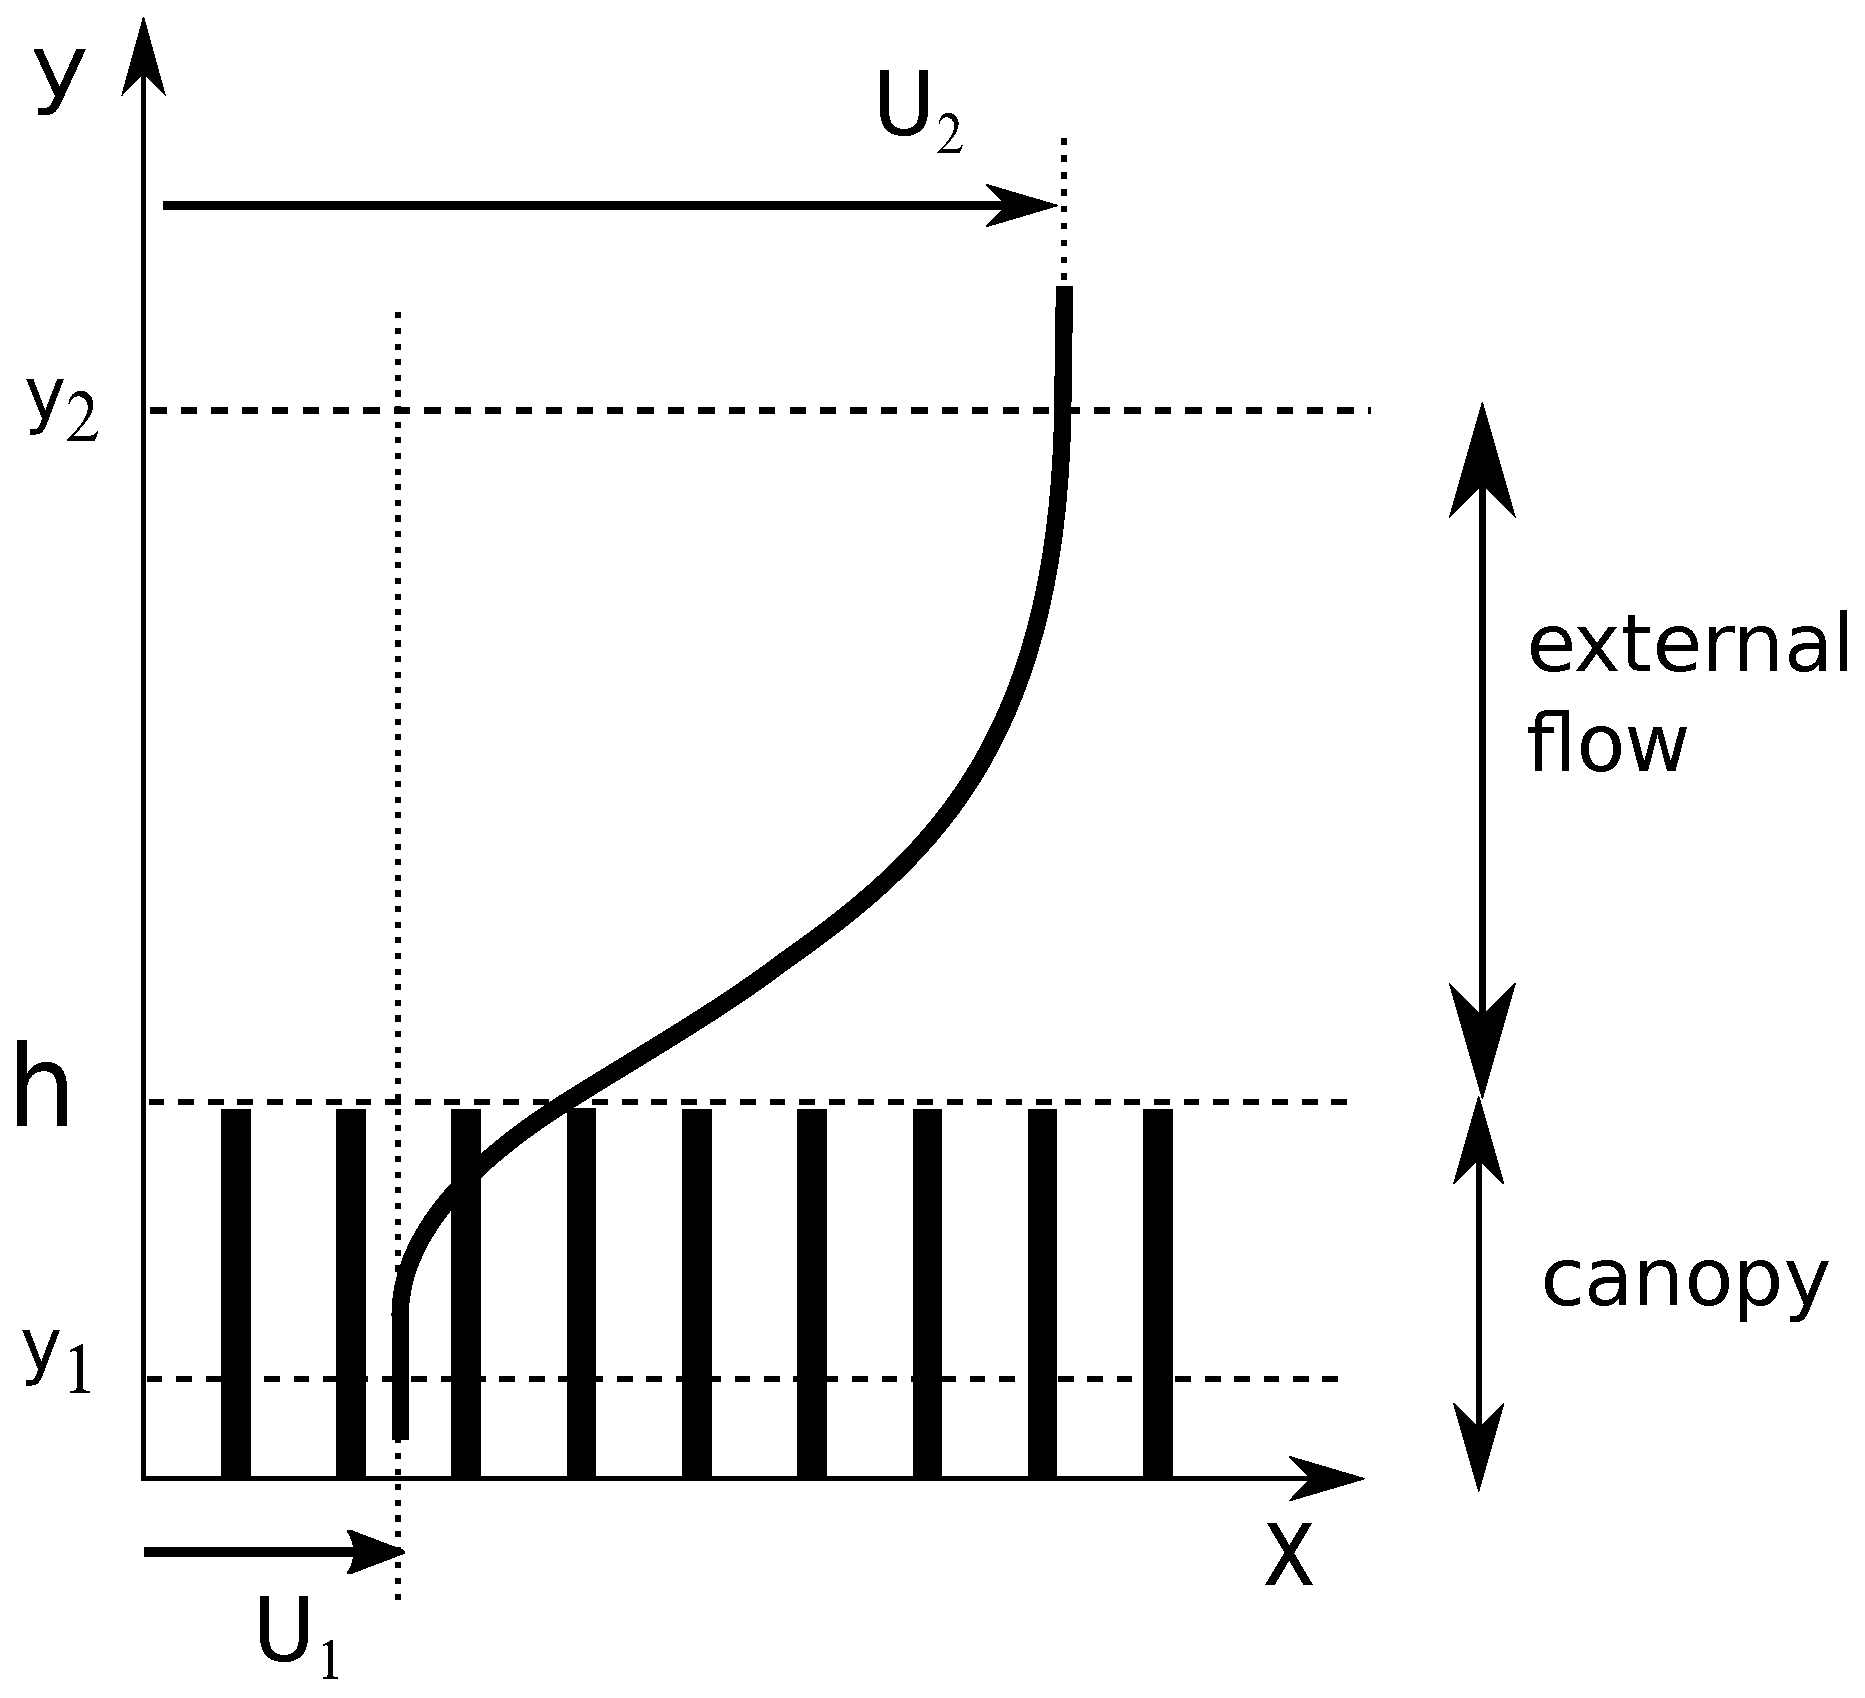
\includegraphics[width=0.8\linewidth]{chapter_3/figure/1}
	\caption{Configuration studied with main notations}
	\label{fig:1}
\end{figure}


\begin{figure}[H]
	\centering
	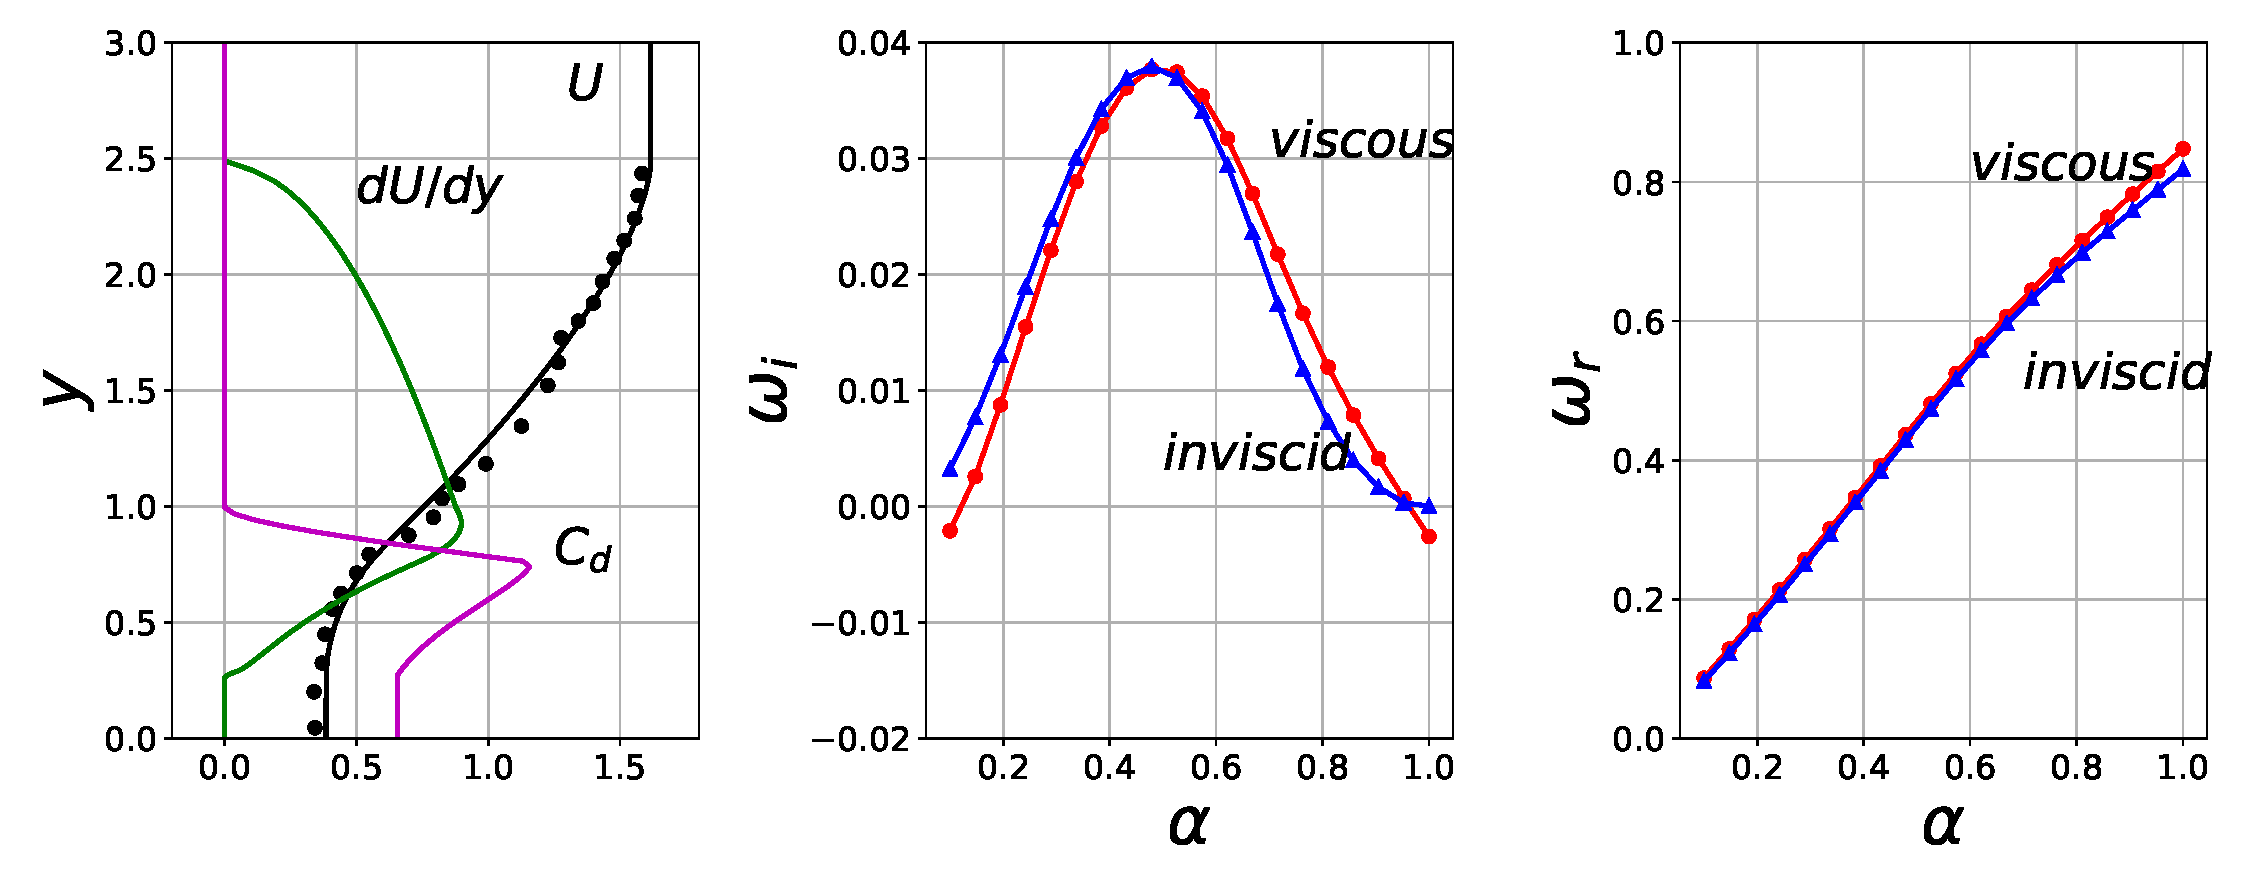
\includegraphics[width=1\linewidth]{chapter_3/figure/2}
	\caption{Left frame: mean flow U , together with experimental data points \cite{ghisalberti2004limited},  its first derivative, and drag coefficient
		distribution (case G). Center: viscous and inviscid growth rates, $\omega_i$ , as a function of the streamwise wavenumber $\alpha$. Right:
		corresponding frequencies, $\omega_r$}
	\label{fig:2}
\end{figure}

to $10^{-4}$; such a slope provides the driving force for the motion. The viscous term is small compared to
the turbulent diffusion term, so that the mean streamwise momentum equation can be approximated
by

\begin{equation}
gS = \derp{\overline{u'v'}}{y} + \frac{1}{2} C_D(y) a {U(y)}^2 
\label{eq:1}
\end{equation}

with $g$ the acceleration of gravity and $C_d$ an isotropic drag function available from the experiments,
variable across the canopy and equal to zero when $y \geq h$. The Reynolds stress $\overline{u'v'}$ is modelled with
the Boussinesq assumption, introducing a turbulent viscosity which depends on a mixing length and
on the gradient of the mean velocity U. Referring to \cite{ghisalberti2004limited} for details of the empirical
correlations used to close the equations and the solution method, we limit ourselves here to stating
that the results obtained for the mean flow are very close to those reported in \cite{zampogna2016instability} (cf.
their Figure 3) and closely match experimental points for the cases G, H, I, and J considered (we use
the same terminology of\cite{ghisalberti2002mixing} \cite{ghisalberti2004limited} \cite{ghisalberti2005mass} to indicate the different flow configurations). An
example of mean flow is reported in \ref{fig:2} (left frame). There, one can observe the computed flow
(against discrete measurement points), its first derivative, and the drag coefficient distribution for one
representative case (experiment G), used below also to discuss stability and sensitivity results.
Other procedures have been employed in the past to calculate the mean flow, with satisfactory
results. For example,\cite{singh2016linear} have considered a constant value of $C_d$ through the canopy, while
\cite{zampogna2016instability} have coupled, at a fictitious interface, the fluid equations outside the canopy
to Darcy’s law within the vegetation. Thus, for the purposes of the present paper, the mean flow is
assumed as given; it could be, for example, simply a fit through experimental data. Nonetheless, in
Appendix A we provide some considerations on how $C_d$ affects the mean flow in the model used here.


%%%%%%%%%%%%%%%%%%%%%%%%%%%%%%%%%%%%%%%%%%%%%%%%%%%%%%%%%%%%%%%%%%%%%%
\subsection{Stability and sensitivity equations}
%%%%%%%%%%%%%%%%%%%%%%%%%%%%%%%%%%%%%%%%%%%%%%%%%%%%%%%%%%%%%%%%%%%%%%
\label{sec2b}
A temporal linear stability analysis is carried out, with the generic perturbation $q'(x, y,t)$ of the
form

\begin{equation}
q'(x,y,y,t)=\tilde q(y){\rm e}^{i(\alpha \  x -\omega \ t)}
\label{eq:q}
\end{equation}

with $\alpha$ the real streamwise wavenumber and $\omega$ a complex number whose real part, $\omega_r$ , is the fre-
quency of the mode and the imaginary part, $\omega_i$ , is the growth rate. The dimensionless linear stability
equations in primitive variables read

\begin{equation}
\begin{split}
& i\alpha u + D v =0,  \qquad D=d/dy \vspace{0.3cm}\\
& \left [ i (\alpha U -\omega)   - \frac{D^2-\alpha^2}{Re}+ a C_d U \right] u + U' v + i \alpha p  = 0,  \qquad U'=\dfrac{d U}{dy} \vspace{0.3cm} \\
& \left[ i (\alpha U -\omega)   - \frac{D^2-\alpha^2}{Re} \right ] v + D p   = 0
\label{eq:uvp}
\end{split}
\end{equation}

with the perturbation velocity components which vanish when $y=0$ and $y_{\infty}$. The upper boundary
of the computational domain is taken far enough away from the lower boundary to ensure that the
results do not vary upon modifications of $y_{\infty}$ . All the terms in the equations are dimensionless; the
mean speed through the shear layer, $U_m = \dfrac{U_1 +U_2}{2}$ , is used to scale the disturbance velocity components, pressure is scaled with
$\rho {U_m}^2$ , distances with $h$, and time with $h/U_m$ . The Reynolds number
in the equations above is thus defined as $Re = \rho U_m/ \mu h$ , with $\rho$ and $\mu$ the fluid’s density and dynamic
viscosity, respectively. The computations are performed both at the $Re$ values of the experiments
and in the inviscid limit (${Re}^{-1}  \rightarrow 0$ ), for comparison purposes. In the latter case, the boundary
conditions are simply $v = 0$ at $y = 0$ and $y_{\infty}$ .
System \ref{eq:uvp} above and its boundary conditions are, in the following, also written in short
notation as $\mathscr{L} q = 0$. The eigenvalues of the system are those complex values of $\omega$ which yield
non-trivial solutions for $u$, $v$, and $p$. Two numerical collocation codes are written, and success-
fully compared; one is based on the equations in primitive variables form, the second solves an
Orr-Sommerfeld-like equation (with the addition of the drag term) along the lines of \cite{singh2016linear}.
In both cases, a spectral scheme based on N Chebyshev polynomials is used (N is typically equal
to 300 to ensure grid-converged results), with an algebraic mapping between the physical and the
spectral domains (\cite{hussaini1987spectral} ).
Viscous and inviscid stability results for case G are shown in \ref{fig:2} (center and right frames);
differences are small, in consideration of the fact that the Reynolds number of the viscous case
is relatively large ($Re = 3450$). The viscous wavenumber of largest amplification is found for
$\alpha = 0.4790$; the waves are weakly dispersive, particularly at low wavenumbers (an original inter-
pretation of phase and group velocities is proposed in Appendix B). The wavelength of largest
growth is smaller than that found by \cite{zampogna2016instability} which was $0.73$; this is related to the slightly
different base flow in the two cases (in the present contribution a smoothing has been applied to the
$U$ velocity distribution to render $dU/dy$ continuous across $y$) and highlights the sensitivity of this
stability problem to base flow variations.
Following \cite{bottaro2003effect} it is assumed that small variations in base flow and drag coefficient
entail infinitesimal variations in the system’s eigenvalues and eigenfunctions. We stress here the fact
that $C_d$ is identically equal to zero outside of the canopy, and this implies that there are no possible
variations in $C_d$ for $y \geq 1$. The sensitivity functions to variations in $U$ and $C_d$ are obtained by using
the properties of the adjoint system which is defined from the Lagrange identity

\begin{equation}
0 = \delta \langle q^{\dagger}, \mathscr{L} q \rangle = 
\langle q^{\dagger}, \mathscr{L} \delta q \rangle +
\langle q^{\dagger}, \derp{\mathscr{L}}{U}  q \delta U\rangle +
\langle q^{\dagger}, \derp{\mathscr{L}}{C_d}  q \delta C_d\rangle +
\langle q^{\dagger}, \derp{\mathscr{L}}{\omega}  q \rangle \delta \omega
\label{eq:lagid}
\end{equation}

\begin{figure}[H]
	\centering
	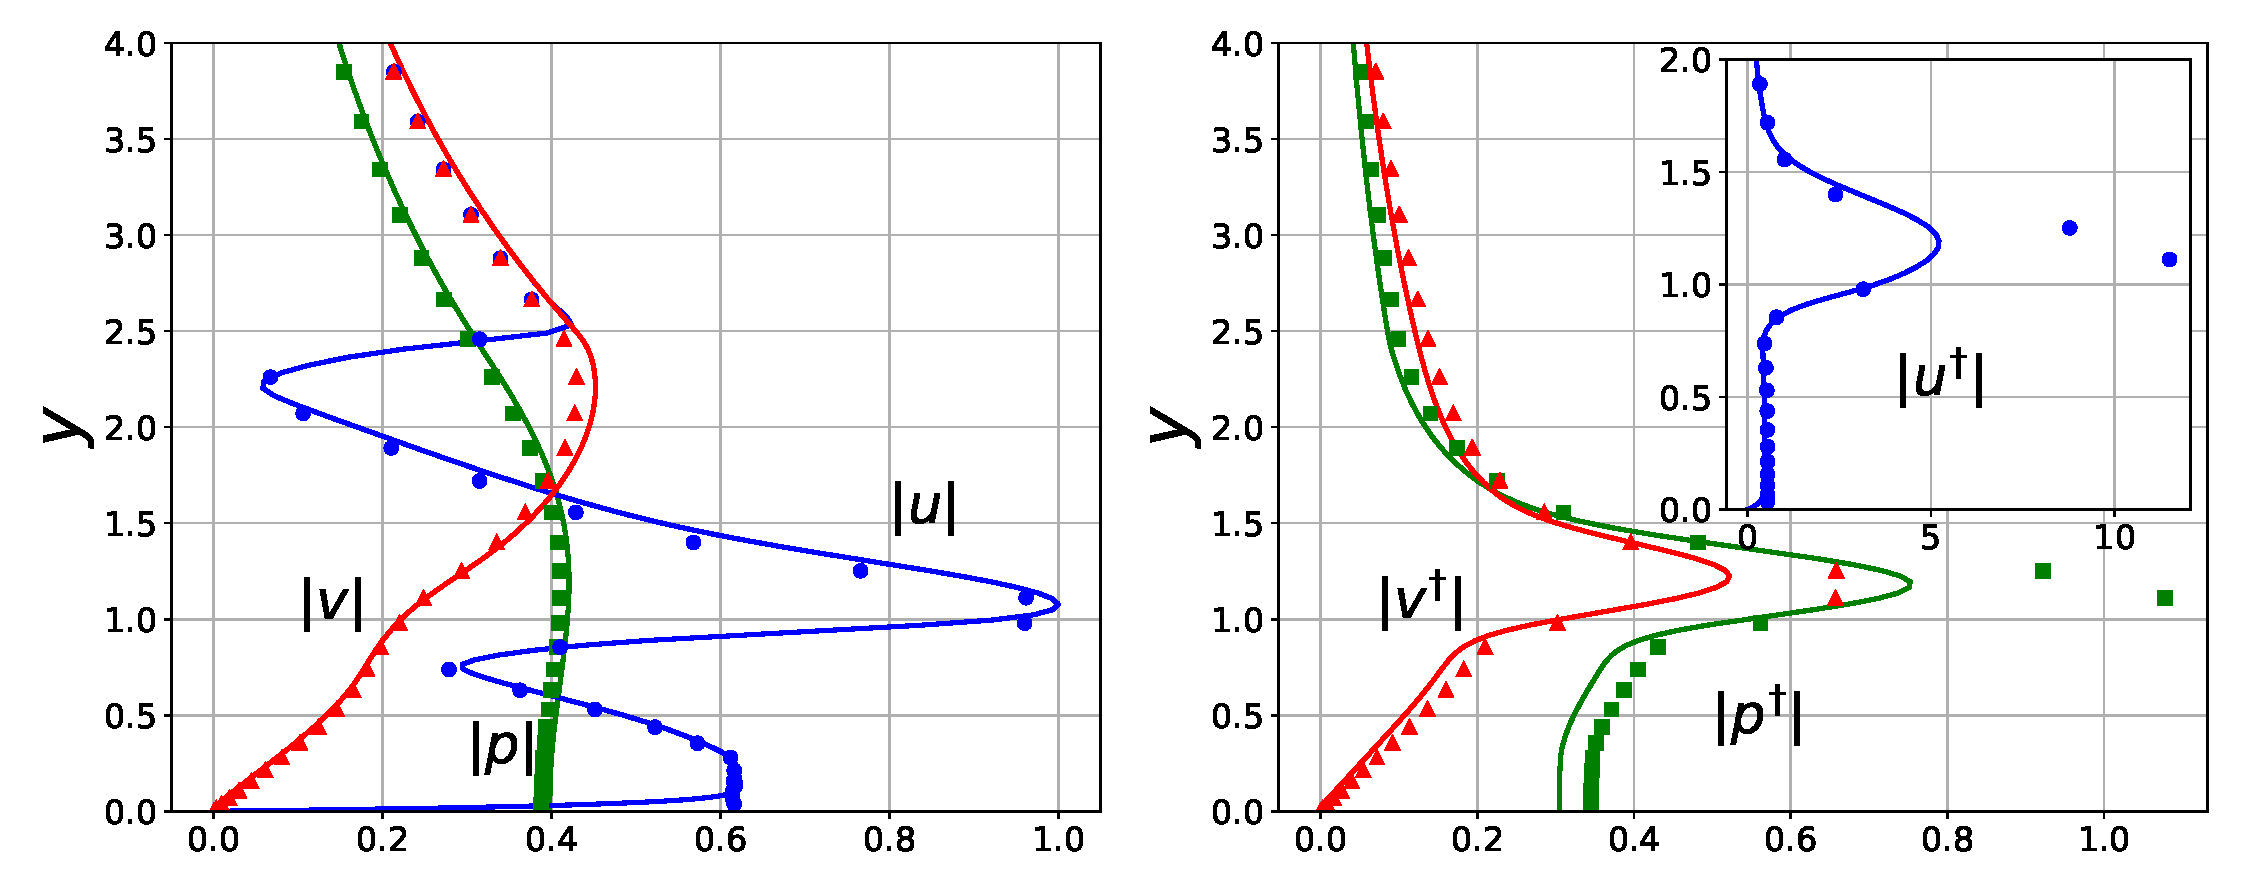
\includegraphics[width=1\linewidth]{chapter_3/figure/3}
	\caption{Moduli of direct (left frame) and adjoint (right frame) eigenfunctions for the viscous (continuous lines, $Re = 3450$)
		and the inviscid (symbols) case, in correspondence to the wavenumber of largest amplification.}
	\label{fig:3}
\end{figure}

and considering the effect of independent variations of $U$ and $C_d$ onto $q$ and $\omega$. It is found that

\begin{equation}
\delta \omega =\delta \omega_r + i \delta \omega_i= \int_0^{y_{\infty}}  G_U(y) \delta U(y) dy + \int_0^{1}  G_{C_D}(y) \delta C_D(y) dy
\label{eq:s_omega}
\end{equation}

with

\begin{equation}
\begin{split}
&G_{U} =  \alpha \left[ \overline{v^{\dagger}} v + \overline{u^{\dagger}} u  \right] +i   (\overline{u^{\dagger}}   v)' -i a C_d \overline{u^{\dagger}}  u \vspace{0.3cm}\\
&G_{C_D} =  - i \alpha  U  \overline{u^{\dagger}} u
\label{eq:GCD}
\end{split}
\end{equation}

the required sensitivity functions; the real parts of $G_U$ and $G_{C_d}$ express sensitivities to variations in
the frequency of the mode while the imaginary parts are sensitivities to variations in the growth rate.
Direct and adjoint eigenfunctions are normalized so that $N_{\omega} = 1$, with

\begin{equation}
N_{\omega} = \int_0^{y_{\infty}} \left[ \overline{ v^{\dagger}} v  +  \overline{ u^{\dagger}} u \right] dy
\label{eq:norm}
\end{equation}

An example of direct and adjoint eigenfunctions is provided in \ref{fig:3}, both in the viscous case
($Re = 3450$) and in the inviscid limit, for $\alpha = 0.4790$. It is interesting to observe that while the
direct eigenfunctions are almost overlapped, the same is not the case for the adjoint eigenfunctions,
with the inviscid mode (drawn with symbols) which has a larger amplitude than the viscous one.
The shapes of the direct eigenfunctions are very close to those reported in \cite{zampogna2016instability}. The adjoint modes
reveal that the flow is most sensitive to streamwise forcing, particularly when it occurs slightly
above the edge of the canopy. Source terms in the mass conservation and in the vertical momentum
equations are much less effective.


%%%%%%%%%%%%%%%%%%%%%%%%%%%%%%%%%%%%%%%%%%%%%%%%%%%%%%%%%%%%%%%%%%%%%%
\section{SENSITIVITY RESULTS FOR THE ISOTROPIC DRAG MODEL}
%%%%%%%%%%%%%%%%%%%%%%%%%%%%%%%%%%%%%%%%%%%%%%%%%%%%%%%%%%%%%%%%%%%%%%
\label{sec:3}

Some representative sensitivity functions are plotted in \ref{fig:4}; viscous and inviscid results
concur in showing that the largest sensitivities to variations of U are found right above the vegeta-
tion’s edge, where there are peaks in the adjoint eigenfunctions and where $d^2 U/d y^2$ vanishes. The
$U$-sensitivities are negligible within the vegetated layer and for values of $y$ larger than twice the
canopy’s height. The $C_d$-sensitivities are non-negligible only in close proximity of the interface.
It is interesting to observe that real and imaginary parts of the $U$-sensitivity functions are
shifted in y with respect to one another; this means that, for example, a localized perturbation at
a given $y$ position (above the canopy) might have a strong repercussion on the growth rate but not
on the frequency of the most unstable Kelvin-Helmholtz mode, or vice versa. Comparing left and
right frames of the figure, it is seen that inviscid $G_U$ sensitivity functions display sharper peaks and
steeper gradients, and yield larger variations in $\omega$ than their viscous counterparts in the proximity of
the $U$ inflection point, a clear consequence of the inviscid mechanism ruling the instability. In both
the viscous and the inviscid models, the sensitivity to base flow variations is typically one order of
magnitude larger than the sensitivity to changes in the drag coefficient.

\begin{figure}[H]
	\centering
	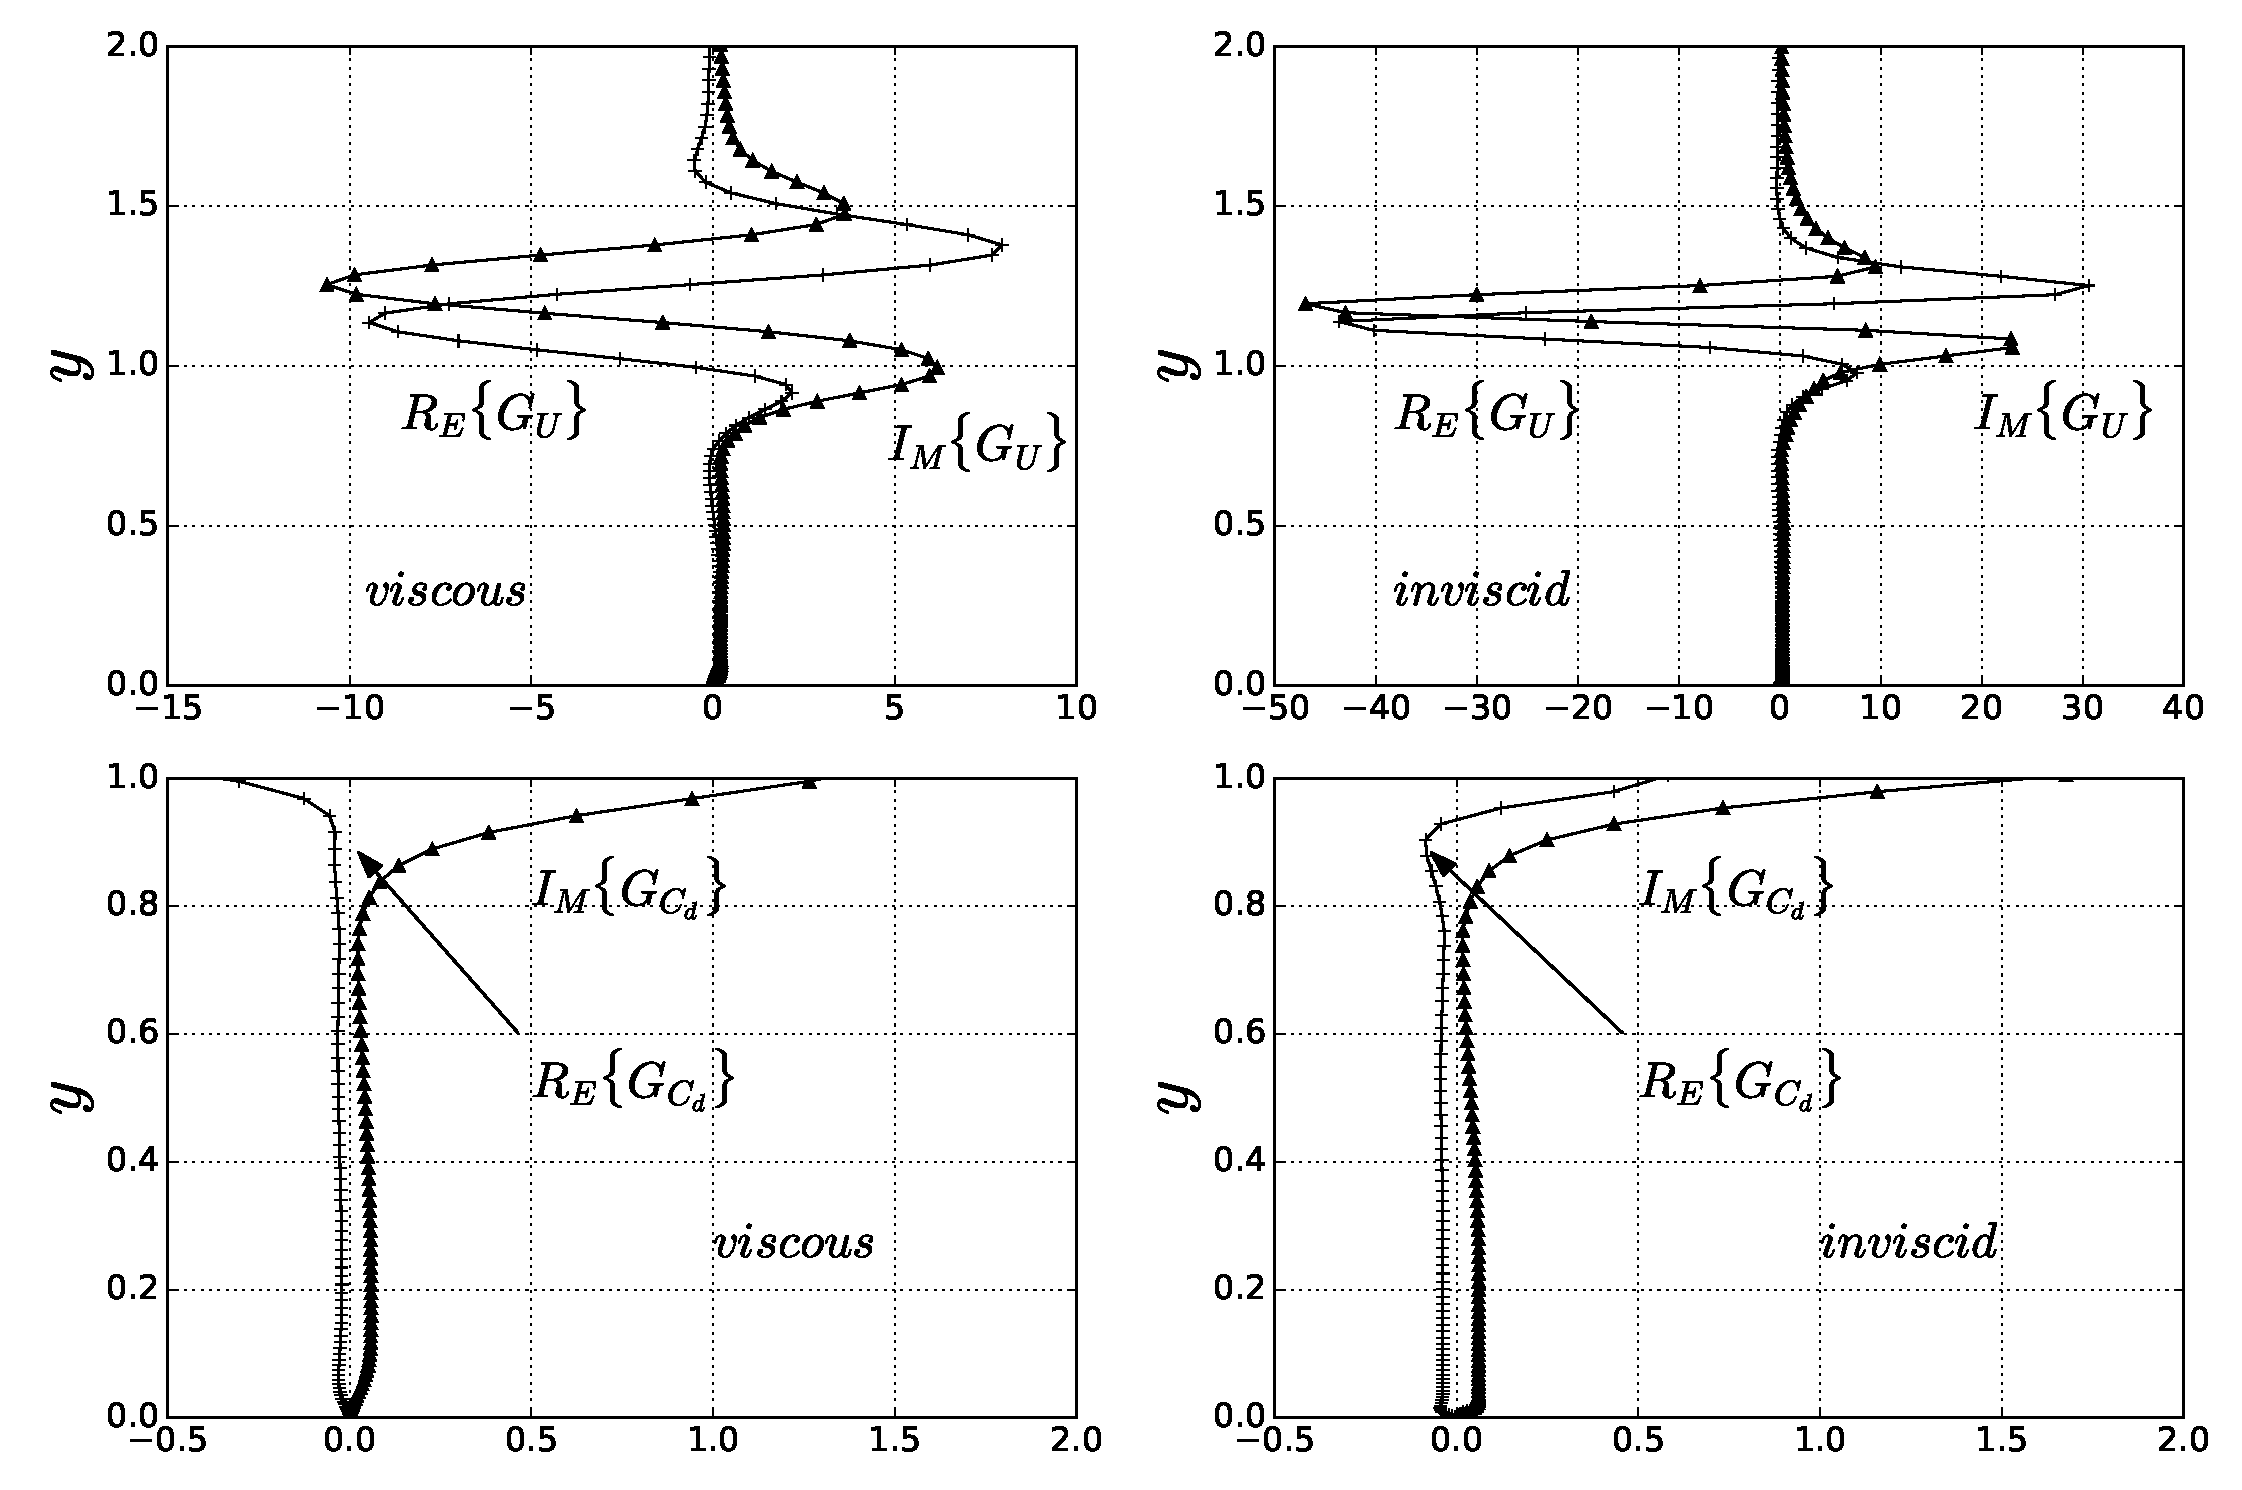
\includegraphics[width=1\linewidth]{chapter_3/figure/4}
	\caption{Real and imaginary parts of the sensitivities to mean flow variations (top) and to variations in the drag distribution
		function (bottom), for the parameters of \ref{fig:3}}
	\label{fig:4}
\end{figure}

The infinite norm of the sensitivities for the four cases studied (G, H, I, and J) is reported in
\ref{fig:5}; the main result found is that ${|G_U|}_{\infty}$ grows monotonically with $\alpha$ (and more so in the inviscid
case) whereas ${|G_{C_d}|}_{\infty}$ does not. It is consistently found that ${|G_U|}_{\infty}$ of case H is larger than that of
case I, which exceeds the corresponding value of case J, in turn larger than${|G_U|}_{\infty}$ of case G. This is
not unexpected in view of the values of the mean shear $\dfrac{U_2 - U_1}{H}$  which are, going from H to G, equal

\begin{figure}[H]
	\centering
	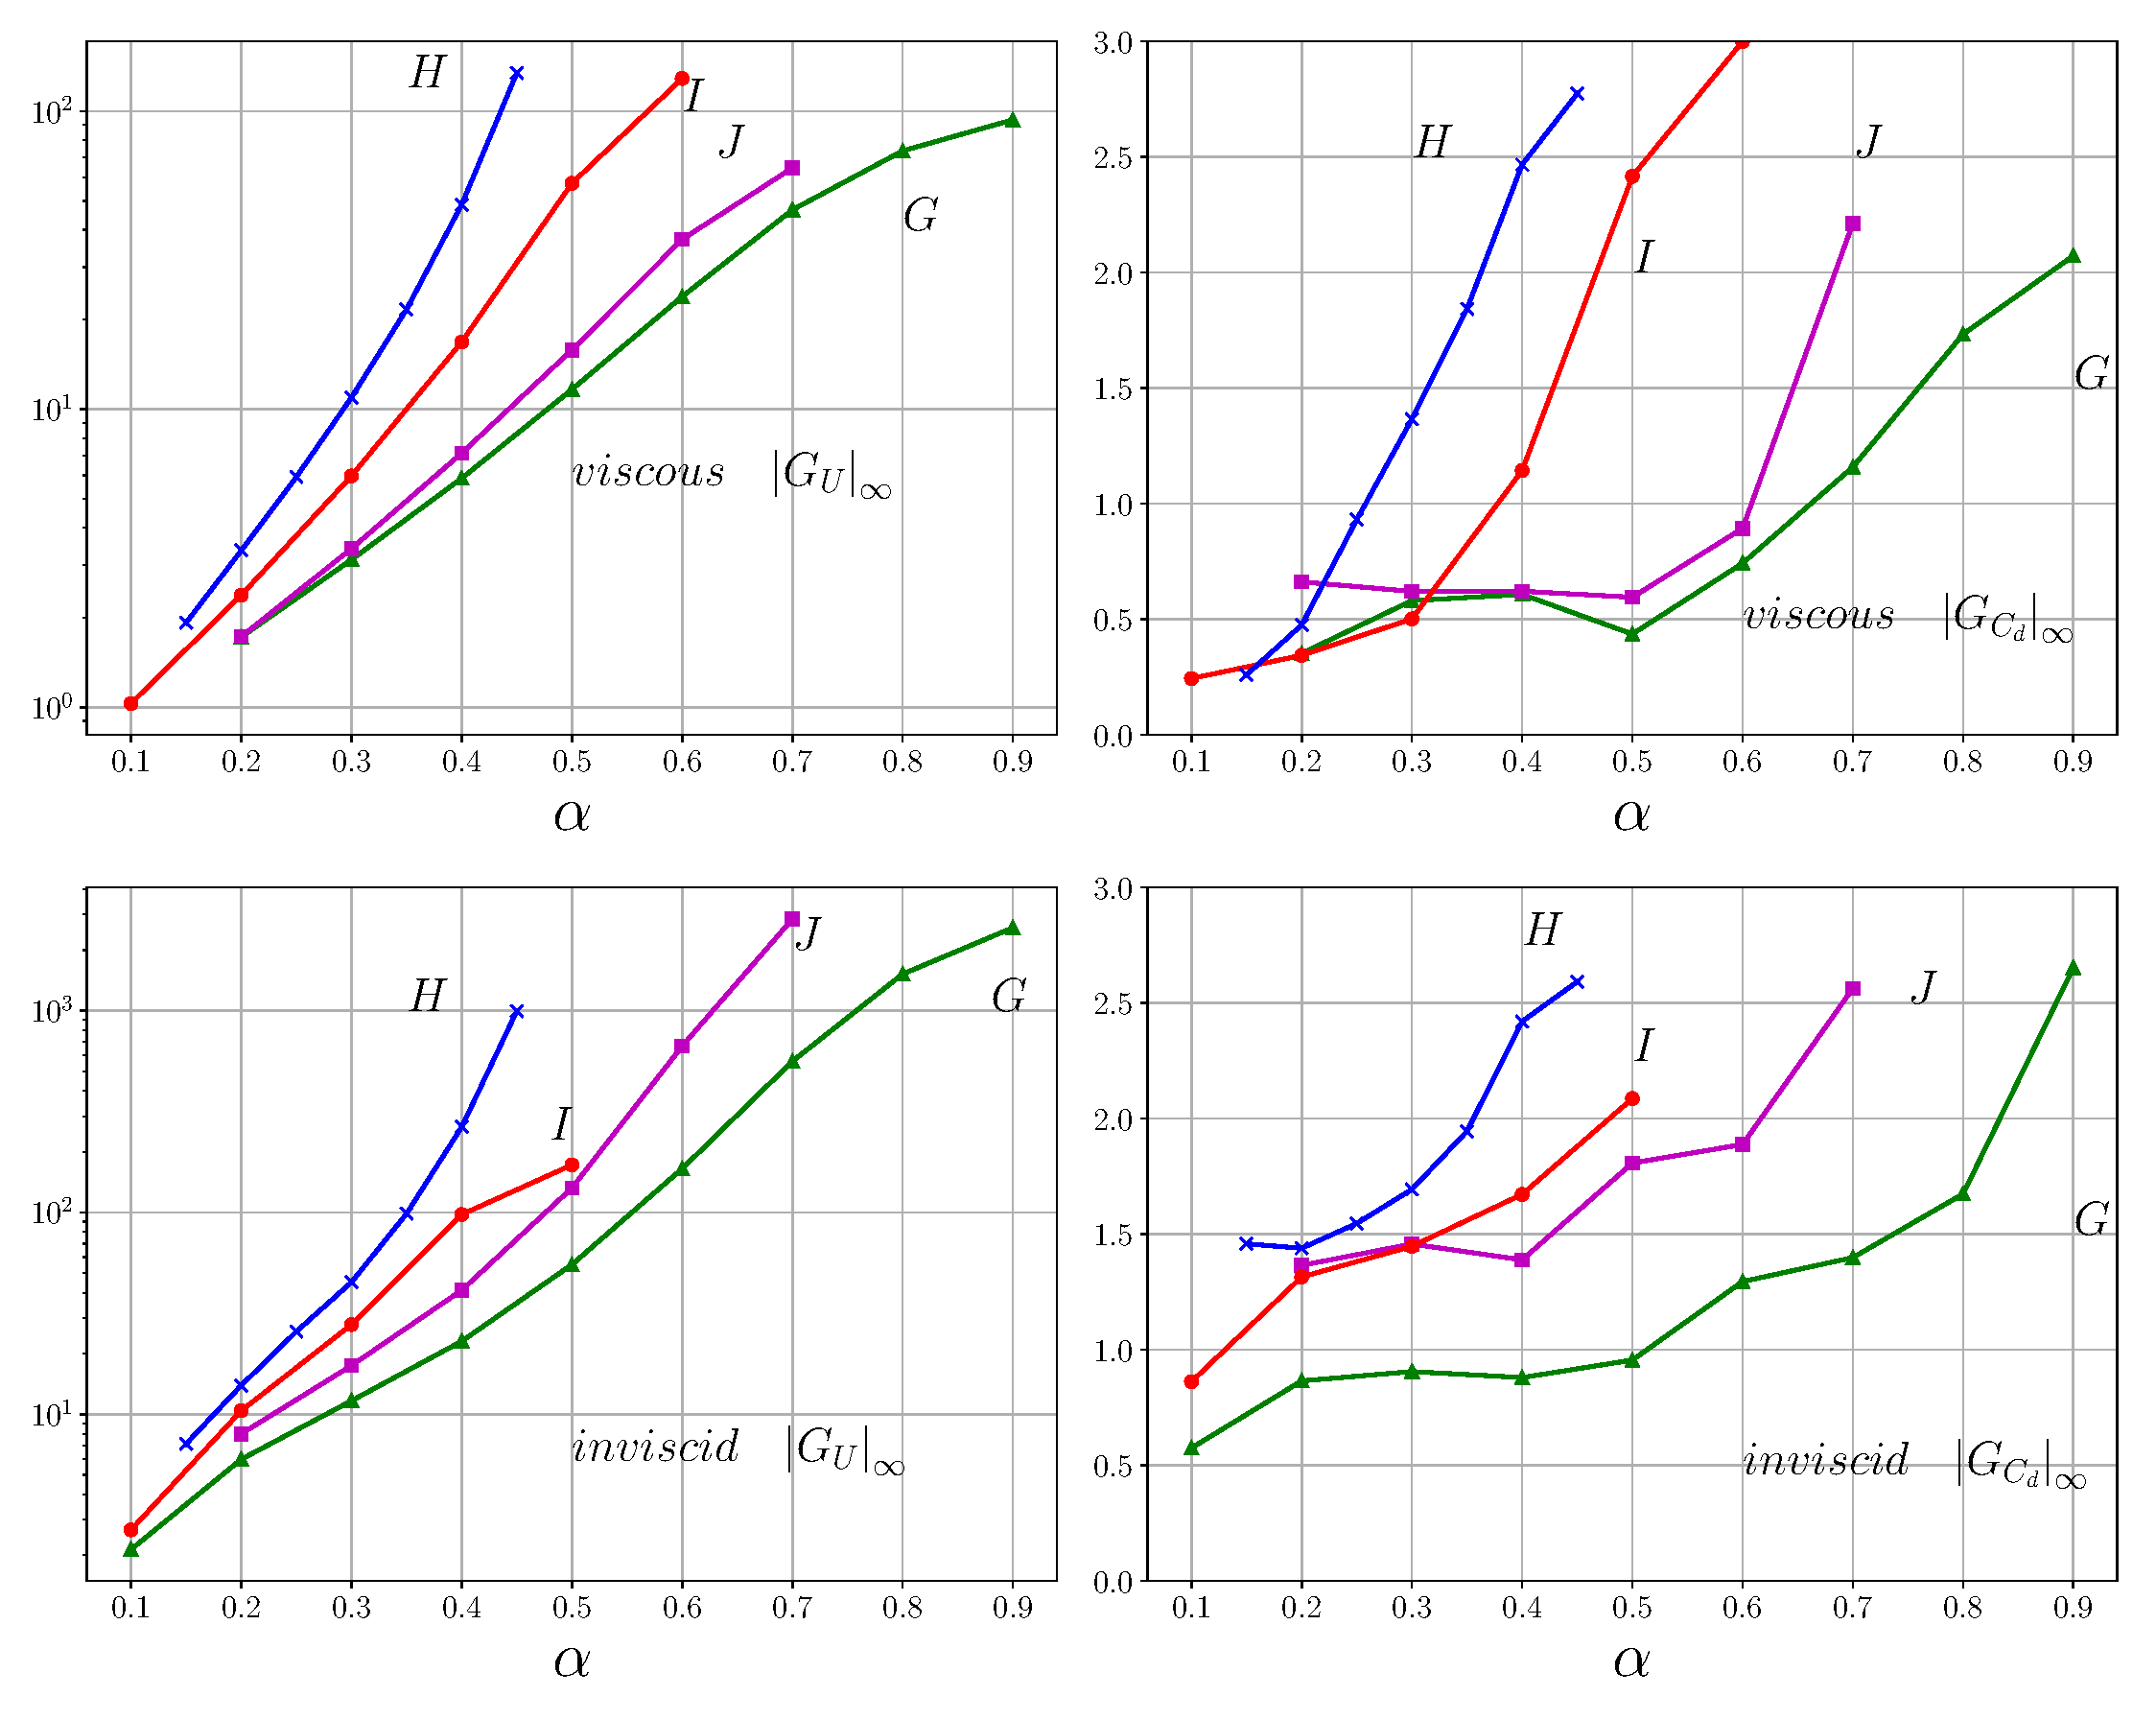
\includegraphics[width=1\linewidth]{chapter_3/figure/5}
	\caption{Infinite norms of the sensitivity functions for varying $\alpha$}
	\label{fig:5}
\end{figure}

to $0.236$, $0.158$, $0.084$, and $0.071 s^{-1}$ , respectively. The sensitivity of the eigenvalue $\omega$ to variations
in the mean flow is generally stronger than the corresponding sensitivity to variations in the drag
coefficient (aside for the long wave limit, where they are comparable). This might be interpreted
positively, considering that the use of a scalar coefficient $C_d$ to represent the drag within the canopy
is but a crude approximation. An alternative model to represent the flow throughout a network of
rigid, cylindrical dowels has recently been proposed by \cite{zampogna2016instability} The sensitivity results for
such a new model are discussed next.


%%%%%%%%%%%%%%%%%%%%%%%%%%%%%%%%%%%%%%%%%%%%%%%%%%%%%%%%%%%%%%%%%%%%%%
\section{AN ALTERNATIVE SENSITIVITY MODEL: ACCOUNTING FOR THE CANOPY ANISOTROPICITY}
%%%%%%%%%%%%%%%%%%%%%%%%%%%%%%%%%%%%%%%%%%%%%%%%%%%%%%%%%%%%%%%%%%%%%%
\label{sec:4}

The stability problem in this section is based on the coupling between two regions, one outer
region dominated by inertia and ruled by the inviscid equations and an inner one dominated by
viscosity and ruled by Darcy’s law, with account of the canopy geometry through a tensorial
permeability, as described by \cite{zampogna2016instability} Normalizing the disturbance equation which couples
pressure and velocity in the inner region with the same scales as previously, we obtain

\begin{equation}
{u_i}' = -Re \dfrac{d}{ah^2} \mathcal{K}_{ij} \derp{p'}{{}x_j}',  \qquad (x_1, x_2) = (x,y)
\label{eq:darcy}
\end{equation}


with $\mathcal{K}_{ij}$ the dimensionless permeability. The effective interface between the inertial region and the
slow, viscosity-dominated region does not coincide with the edge of the canopy; in fact, the rapid
outer flow penetrates through the upper part of the vegetation and an effective matching between
outer and inner flows must be enforced some distance $\delta$ below the canopy’s edge \cite{le2006interfacial}.  This distance,
a penetration depth, has been successfully computed by \cite{zampogna2016fluid} for a few cases
and is found to increase with the Reynolds number of the flow; for experiment G discussed below it
is$ \delta = 0.40$ \cite{zampognaprivate}. On account of the results shown in \ref{fig:4}, with the sensitivities which are negligible
for $y \approx 0.60$, we expect that the exact position of the effective interface will not affect the results
significantly.
Using the fact that the velocity within the orthotropic porous medium is divergence free, the
interface condition to be applied at $y_{itf} = 1 - \delta$ is found to be \ref{eq:darcybc}

\begin{equation}
v|_{itf} + B(\alpha) p|_{itf} = 0
\label{eq:darcybc}
\end{equation}

with

$$
B(\alpha) = Re \dfrac{d}{ah^2} \sqrt{\mathcal{K}_{11}\mathcal{K}_{22}} \alpha \tanh (\theta), \qquad \theta = \alpha \sqrt{\dfrac{\mathcal{K}_{11}}{\mathcal{K}_{22}}}  y_{itf}
$$

The second boundary condition that the Rayleigh stability equation must satisfy at $y_{\infty}$ is sim-
ply $v = 0$. Thus, we solve only for the inviscid flow in the outer region, and the permeability
of the inner domain enters the equations only through the interface condition \ref{eq:darcybc}. $\mathcal{K}_{ij}$ is a two-
by-two diagonal tensor; $\mathcal{K}_{11}$ is the component of the dimensionless permeability along $x$ and
$\mathcal{K}_{22}$ is the $y$ component. For case G considered here, the packing density of the elements is
$a = 0.04 cm^{-1}$ ; it is also found that $\mathcal{K}_{11}= 0.0512$ and $\mathcal{K}_{22} = 0.0575$ \cite{zampognaprivate},  so that the function $B(\alpha)$
reads $B = 15.727 \alpha \tanh (0.566 \alpha)$.


%%%%%%%%%%%%%%%%%%%%%%%%%%%%%%%%%%%%%%%%%%%%%%%%%%%%%%%%%%%%%%%%%%%%%%
\subsection{The sensitivity equations}
%%%%%%%%%%%%%%%%%%%%%%%%%%%%%%%%%%%%%%%%%%%%%%%%%%%%%%%%%%%%%%%%%%%%%%

The adjoint equations in this case are the same as system \ref{eq:uvp}, without the terms containing $1/Re$
and $C_d$ , and the boundary conditions are

\begin{equation}
v^{\dagger}|_{itf} - B(\alpha) p^{\dagger}|_{itf} = 0, \qquad v^{\dagger}|_{y_{\infty}} = 0
\label{eq:darcybc_adjoint}
\end{equation}

The variation in the complex frequency is related to variations in the mean flow and in the perme-
ability components through the equation

$$
\delta \omega = \int_{y_{itf}}^{y_{\infty}}  G_U(y) \delta U(y) dy + G_{\mathcal{K}_{11}} \delta \mathcal{K}_{11} + G_{\mathcal{K}_{22}} \delta \mathcal{K}_{22}
$$

\begin{figure}[H]
	\centering
	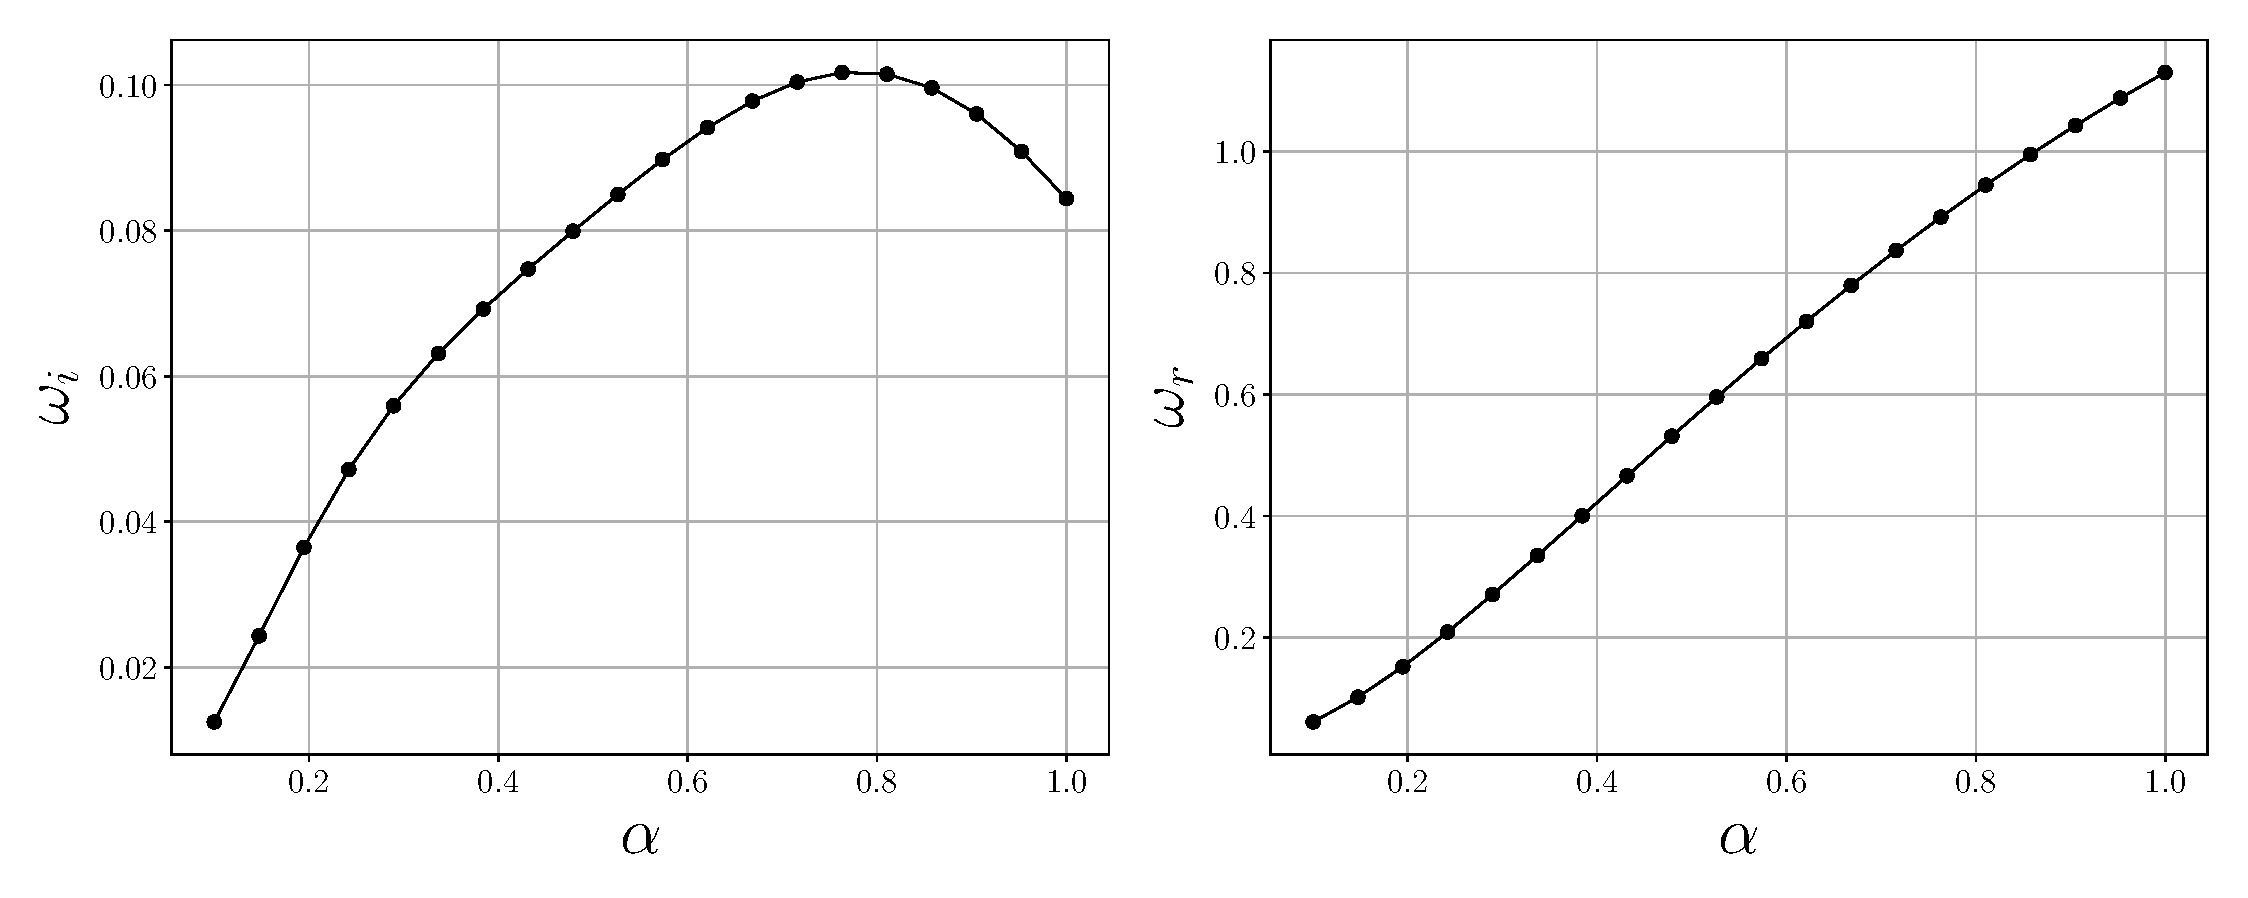
\includegraphics[width=1\linewidth]{chapter_3/figure/6}
	\caption{Amplification factor (left) and frequency of the most unstable mode as a function of $\alpha$, for the anisotropic drag
		model}
	\label{fig:6}
\end{figure}


with

\begin{equation}
\begin{split}
& G_U = \alpha  \left[  \overline{v^{\dagger}} v +  \overline{u^{\dagger}} u \right] + i ( \overline{u^{\dagger}} v)'  \vspace{0.3cm}\\
& G_{\mathcal{K}_{11}} = -\dfrac{i}{2} \alpha Re \dfrac{d}{a h^2}  \left[  \overline{p^{\dagger}} p \right]|_{itf} \sqrt{\dfrac{\mathcal{K}_{22}}{\mathcal{K}_{11}}} \left\lbrace \tanh \theta + \dfrac{\theta}{\cosh^2 \theta}\right\rbrace	\vspace{0.3cm}\\
& G_{\mathcal{K}_{22}} = -\dfrac{i}{2} \alpha Re \dfrac{d}{a h^2}  \left[  \overline{p^{\dagger}} p \right]|_{itf} \sqrt{\dfrac{\mathcal{K}_{11}}{\mathcal{K}_{22}}} \left\lbrace \tanh \theta - \dfrac{\theta}{\cosh^2 \theta}\right\rbrace
\end{split}
\end{equation}


the required sensitivities, with the normalization  $\int_{y_{itf}}^{y_{\infty}} \left[  \overline{v^{\dagger}} v +  \overline{u^{\dagger}} u \right] = 1$.
In writing $\delta \omega$ above, we have made the assumption that the mean flow $U$ does not vary at the two extreme points of the
integration domain.
The stability results (for the same parameters as in \ref{fig:2}) are displayed in \ref{fig:6}. As already
observed in \cite{zampogna2016instability}, both the growth rate and the frequency are slightly larger with this model than
with the isotropic resistance model, for all $\alpha$’s, and the most unstable mode is found at a larger
value of $\alpha$ (here $\alpha \approx 0.8$) in better agreement with experimental correlations \cite{zampogna2016instability} \cite{raupach1996coherent}.  Also in this case the
waves are found to be only weakly dispersive.
Eigenfunctions are plotted in \ref{fig:7}, together with the real and imaginary parts of the $G_U$
sensitivity function. As in \ref{fig:3}, the modulus of the $u$ eigenfunction peaks near the edge of the
canopy ( $y = 1$), whereas the adjoint eigenfunctions have a maximum value slightly above. As a
general remark, the shapes of the direct and adjoint modes are quite similar to those found with
the isotropic resistance model; as reported at the end of \ref{sec2b}, it is found that the flow
is most sensitive to streamwise momentum forcing. Also, real and imaginary parts of $G_U$ have a
double-peak structure, like in the isotropic-drag model, but now the largest absolute value of $G_U$ is

\begin{figure}[H]
	\centering
	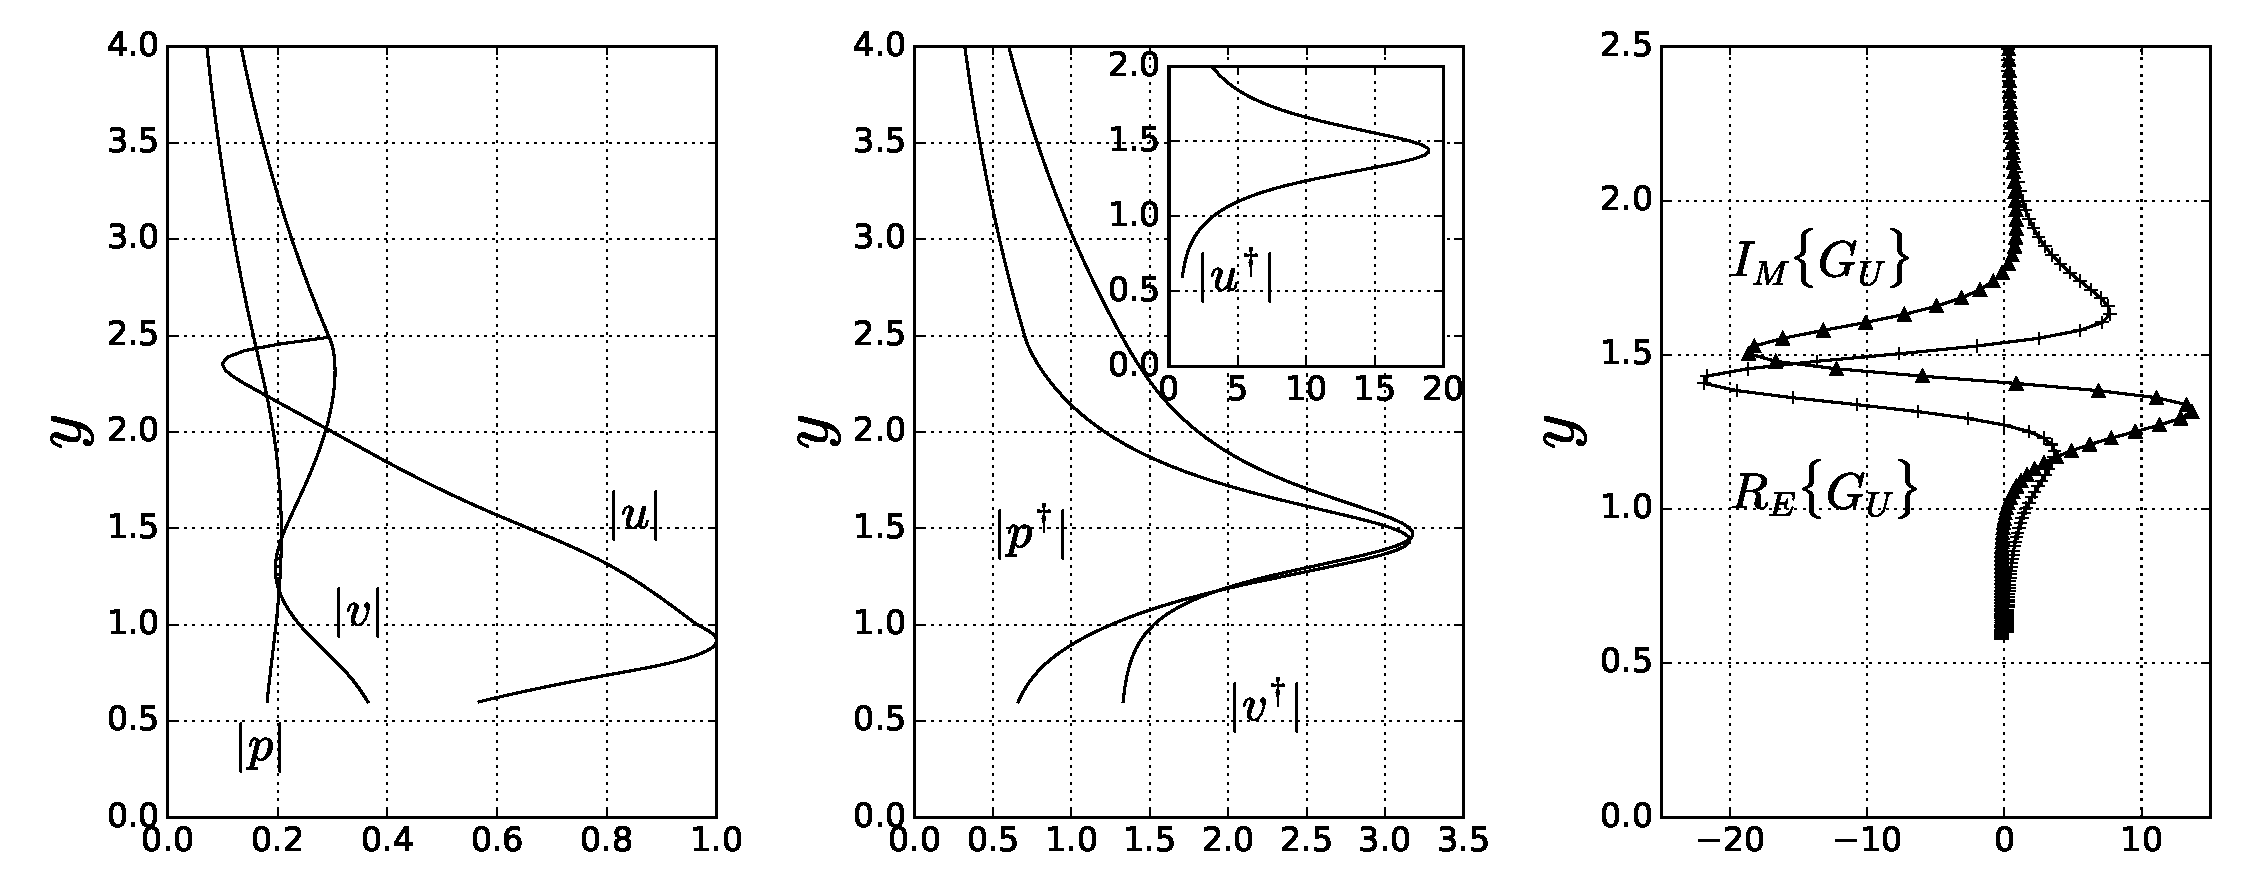
\includegraphics[width=1\linewidth]{chapter_3/figure/7}
	\caption{Left and center frames: moduli of direct and adjoint eigenfunctions; pressure and “adjoint pressure” are drawn with
		dashed lines. Right: real and imaginary parts of the sensitivity function $G_U$ ($\alpha = 0.4790$)}
	\label{fig:7}
\end{figure}

\begin{figure}[H]
	\centering
	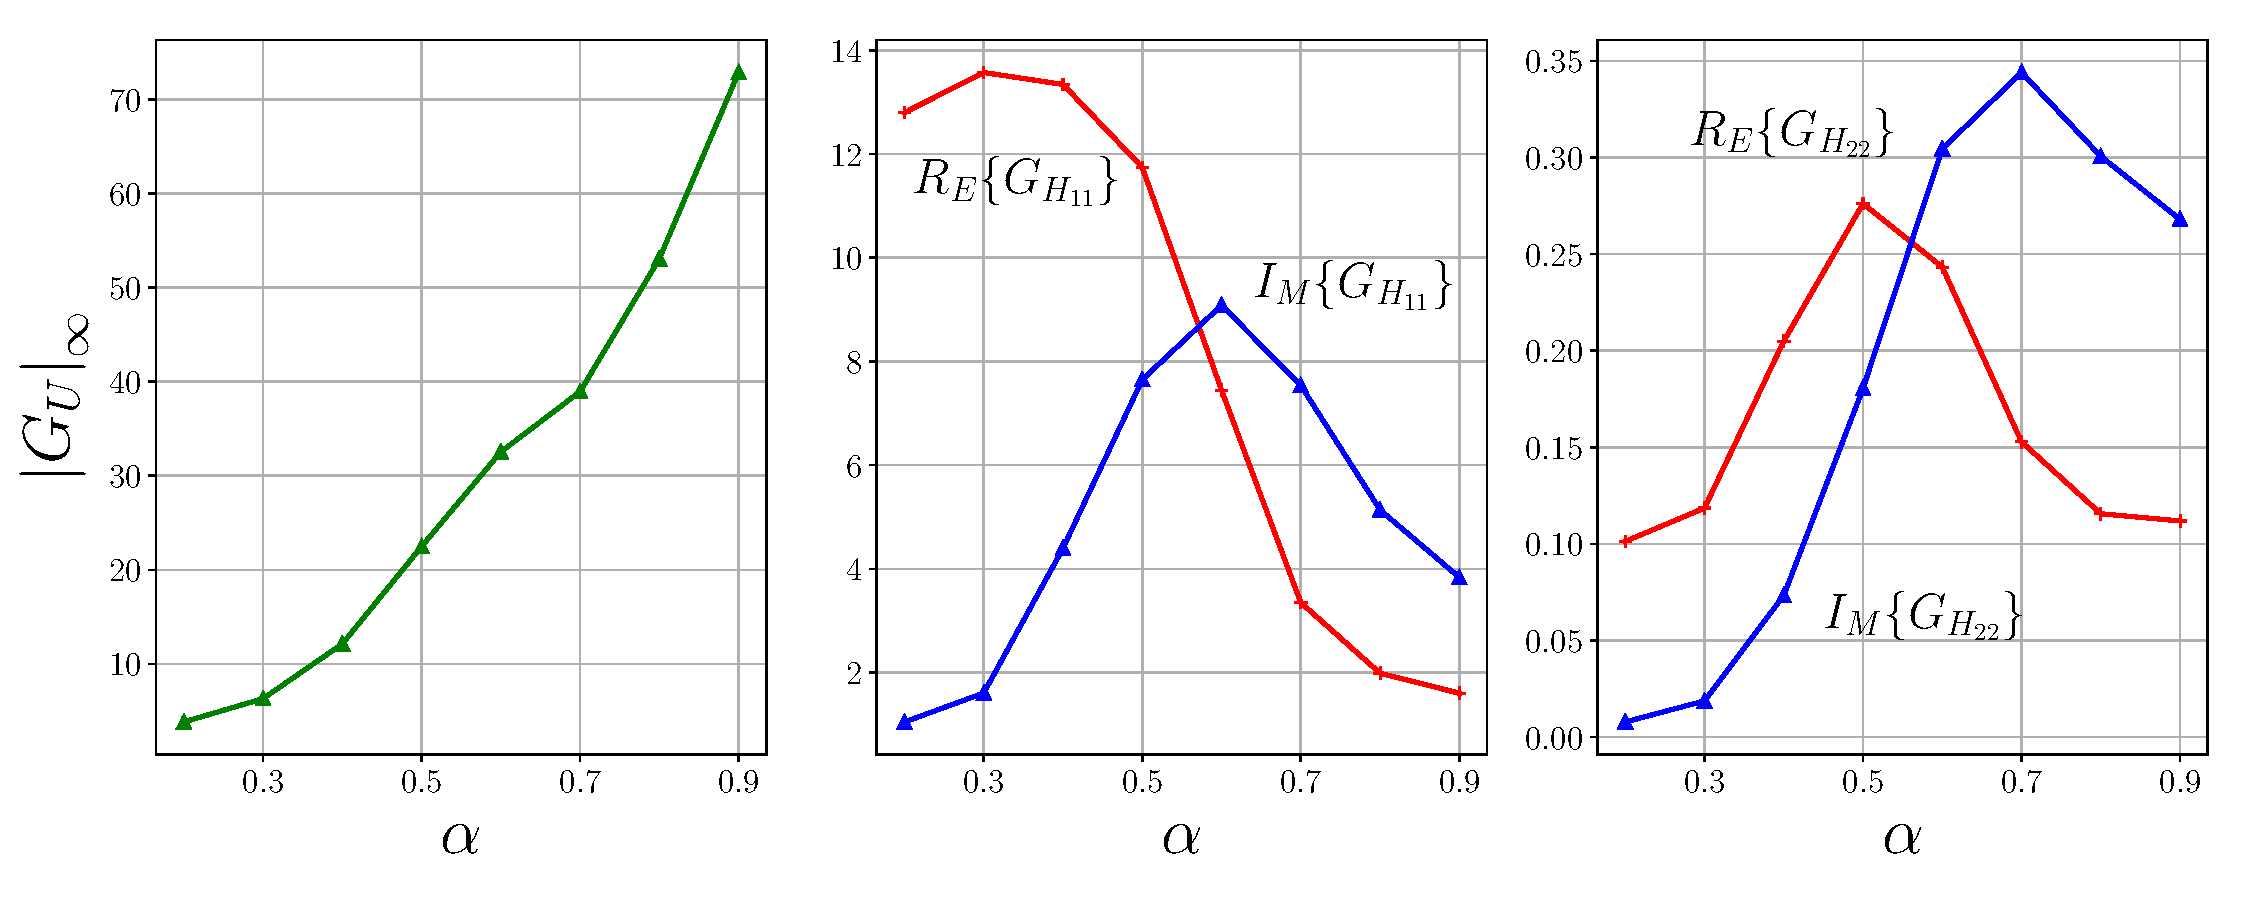
\includegraphics[width=1\linewidth]{chapter_3/figure/8}
	\caption{Case G. Left: infinite norm of $G_U$ for varying $\alpha$. Center and right frames: real and imaginary parts of the sensitivity
		coefficients to variations in the permeability components}
	\label{fig:8}
\end{figure}

smaller and shifted towards a larger y than in the previous inviscid case (cf.\ref{fig:4}, top-right frame).
This can also be appreciated by the inspection of \ref{fig:8} (left); $|G U |_{\infty}$ still grows monotonically with
$\alpha$, but the sensitivity is smaller than that computed earlier (cf. \ref{fig:5}) with either the viscous or
inviscid model (it is actually closer to the viscous sensitivity, as an effect of the interface condition).
Furthermore, it is interesting to observe that both real and imaginary parts of $G_U$ vanish for $y = y|_{itf}$
(cf.\ref{fig:7}, right), and this supports the statement made previously that a small shift in the position
of the effective interface has but a minor influence on the most unstable mode.
The sensitivity coefficients for the two components of the permeability tensors are displayed in
\ref{fig:8} (center and right frames): the present model is more effective to variations in $\mathcal{K}_{11}$ than to $\mathcal{K}_{22}$
as far as modifying the complex eigenfrequency. Significantly, different ranges of wavenumbers
behave differently as far as the variation in $\omega$ is concerned. The frequency $\omega_r$ of long waves (around
$\alpha \approx 0.3$) is more easily modified by acting on $\mathcal{K}_{11}$ (with an almost negligible effect on the growth
rate of the wave); conversely, the growth rate of modes with large values of $\alpha$ is affected efficiently
by variations in the first component of the permeability tensor.

%%%%%%%%%%%%%%%%%%%%%%%%%%%%%%%%%%%%%%%%%%%%%%%%%%%%%%%%%%%%%%%%%%%%%%
\section{CONCLUDING REMARKS}
%%%%%%%%%%%%%%%%%%%%%%%%%%%%%%%%%%%%%%%%%%%%%%%%%%%%%%%%%%%%%%%%%%%%%%
We have considered two different models of the flow through a vegetated layer experienc-
ing Kelvin-Helmholtz destabilization. One model is based on the use of a single drag coefficient
to express the force exerted by the vegetation on the fluid, the second considers the canopy as
an orthotropic porous medium and is based on Darcy’s equation with a tensorial permeability \cite{zampogna2016fluid}. 
Both models have advantages and drawbacks. The main advantage of the first model is that the
drag coefficient can be taken to vary across the canopy; whether this positive consideration, based
on macroscopic experimental measurements \cite{ghisalberti2002mixing} \cite{ghisalberti2004limited} \cite{ghisalberti2005mass},  carries over to the stability problem remains to
be established. The second model, applicable to dense porous media, considers two independent
parameters to express the disturbance flow perpendicular and parallel to the rigid dowels forming
the canopy. Such parameters and components of the transversely isotropic permeability tensor K i j
arise from the solution of a local Oseen problem \cite{zampogna2016fluid}. The drawback of the second model is the
fact that an interface (whether real or effective) appears, and adequate matching conditions must
be enforced there. Despite much work since the seminal contribution by \cite{beaver}, a
consensus on the “best” interface conditions between a pure fluid region and a porous medium has
not yet emerged.
The models have been put to test through a classical sensitivity analysis \cite{bottaro2003effect}. Beyond display-
ing stability results which correspond better to those to be expected from available experimental
correlations \cite{raupach1996coherent} \cite{zampogna2016instability}, the anisotropic model is less sensitive to variations in the base flow (with potentially
larger variations in frequency and growth rate of the instability mode for the case of shorter waves).
As far as a direct comparison between $G_{C_d}$ and $G_{\mathcal{K}_{ii}}$ is concerned, this can hardly be made since
the variables represent different objects; in particular, the pressure drop through the canopy depends
directly on $C_d$ and inversely on the permeability. The present results indicate that the anisotropic
model depends significantly on the value of the apparent \cite{zampogna2016fluid} permeability component $\mathcal{K}_{11}$ , whose
evaluation must thus be conducted carefully. This model is also of interest for further developments,
in particular for the study of instabilities developing over waving canopies. Darcy’s law in this latter
case would need to be modified, as described in \cite{mei2010homogenization} and \cite{zampognaMech}.


%%%%%%%%%%%%%%%%%%%%%%%%%%%%%%%%%%%%%%%%%%%%%%%%%%%%%%%%%%%%%%%%%%%%%%
\section*{Acknowledgment}
%%%%%%%%%%%%%%%%%%%%%%%%%%%%%%%%%%%%%%%%%%%%%%%%%%%%%%%%%%%%%%%%%%%%%%
The authors would like to thank the IDEX Foundation of the University of Toulouse for the
financial support granted to the last author under the project “Attractivity Chairs.” The computations
have been conducted at the CALMIP center, Grant No. P1540. The referees are gratefully acknowl-
edged for their comments leading, in particular, to the correct interpretation of the sensitivity of the
drag coefficient and to the material in Appendix A.



%%%%%%%%%%%%%%%%%%%%%%%%%%%%%%%%%%%%%%%%%%%%%%%%%%%%%%%%%%%%%%%%%%%%%%
\section*{APPENDIX A: EFFECT OF C d ON THE MEAN FLOW}
%%%%%%%%%%%%%%%%%%%%%%%%%%%%%%%%%%%%%%%%%%%%%%%%%%%%%%%%%%%%%%%%%%%%%%

In \ref{sec:2ch3} of the paper it is described how the eigenvalue $\omega$ varies as an effect of indepen-
dent variations of $U$ and $C_d$. However, since $C_d$ is not zero within the canopy and it is used to
compute the mean flow profile $U$, we should in principle have expressed $\delta U$ as $\delta U = \dfrac{dU}{d C_d} \delta C_d$
and considered a single sensitivity function ${G^*}_{C_d} = G_{C_d} + \dfrac{dU}{d C_d} G_U$, instead of the two sensitivities given
in \ref{eq:GCD}. This would have certainly been the appropriate line of action if the mean flow equa-
tion were issued from exact equations, in which case we should have considered also the adjoint
of the base flow equation in our variational problem. However, the mean flow model by \cite{ghisalberti2004limited} contains empirical approximations and parameters, and alternative models \cite{singh2016linear}, \cite{zampogna2016instability} —including
very different ones—have been used successfully in the past to predict the mean field; we have thus
made the choice, in both \ref{sec:3} and \ref{sec:4}, of considering the mean flow as given, and to take
independent variations of $U$ and $C_d$ in the stability analysis to assess the effect of modifications in
either variable.
If we were to find how much the base flow depends on the drag coefficient in this particular
problem, we would need to determine the function $U(C_d)$ and take its derivative. Since both $U$
and  $C_d$ are functions of the space coordinate $y$, the implicit dependence can be found, and we
have plotted it for one case on the left frame of \ref{fig:9}. Clearly, the function $U = f(C_d)$ is not
single-valued and therefore the derivative can be calculated only over two separate $U$ (or, equiva-
lently, $y$) intervals. We have carried out the derivation numerically over each interval, within the
range $0.3 \leq y \leq 1$, and the result is reported on the right frame of \ref{fig:9}. The filled triangle and
circle symbols indicate the two y intervals within the canopy.
We first observe that both the location where $C_d$ is maximum and the shape of the func-
tion $U = f(C_d)$ are strongly correlated to the drag law $C_d(y)$, modeled by \cite{ghisalberti2004limited}


\begin{figure}[H]
	\centering
	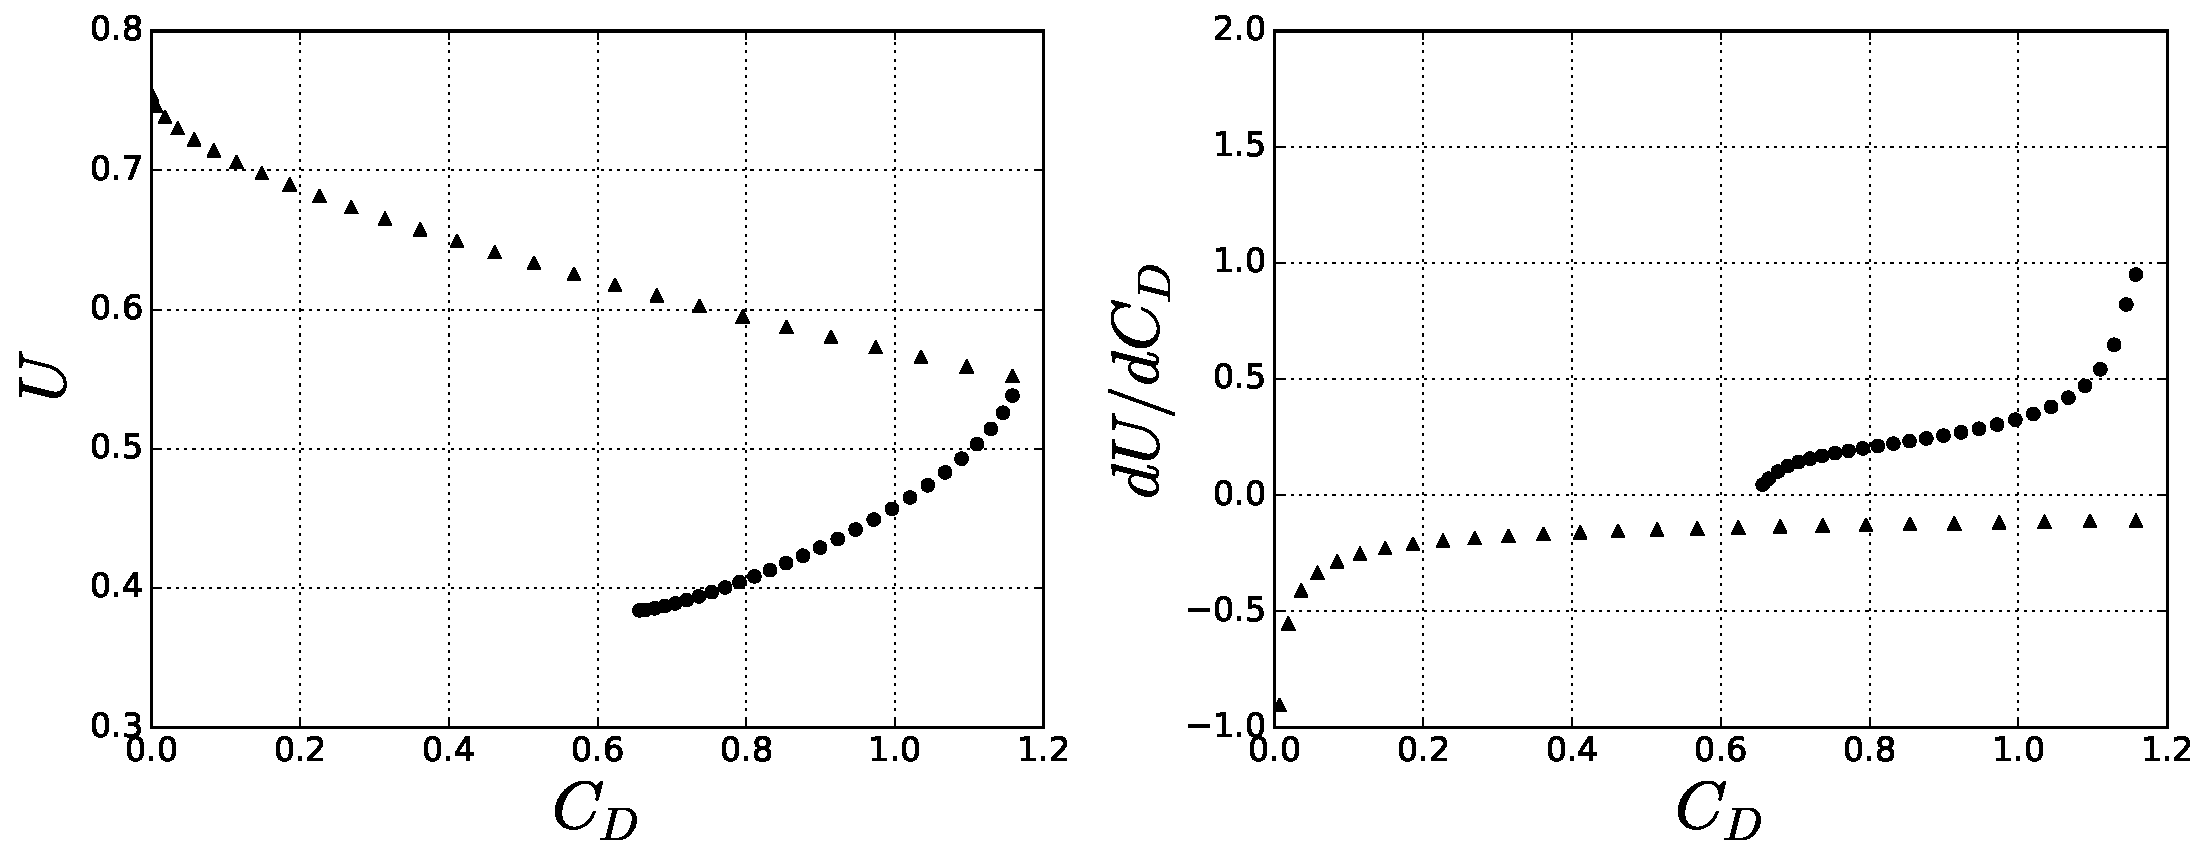
\includegraphics[width=1\linewidth]{chapter_3/figure/9}
	\caption{Case G. Left: mean velocity profile, $U$ , versus the drag coefficient, $C_d$ . Right: first derivative, $dU / d C_d$ . The triangles denote the region $y \in [0.76, 1]$, the filled circles denote the region $y \in [0.3, 0.76]$.}
	\label{fig:9}
\end{figure}

through their measurement data (cf. their Figure 7 and Equation (18)). We also notice that the deriv-
ative $dU/dC_d$ is reasonably small except locally at the point where the derivative of the function is
not continuous, where it is of order 1. The discontinuity there is however artificial since the function
$C_d(y)$ given in Equation (18) of \cite{ghisalberti2004limited}, where $C_d$ is divided into a parabolic and a
linear part, can be easily modified to yield a continuous first derivative at $y = 0.76$ if required, still
maintaining a mean flow very close to the measured one.

%%%%%%%%%%%%%%%%%%%%%%%%%%%%%%%%%%%%%%%%%%%%%%%%%%%%%%%%%%%%%%%%%%%%%%
\section*{APPENDIX B: A DIGRESSION ON SPATIAL STABILITY THEORY AND GROUP VELOCITY}
%%%%%%%%%%%%%%%%%%%%%%%%%%%%%%%%%%%%%%%%%%%%%%%%%%%%%%%%%%%%%%%%%%%%%%

Stability problems such as the first one considered in this paper can be approached with the
spatial theory framework, with the wavenumber $\alpha$ complex, its imaginary part being a growth rate,
and the circular frequency $\omega$ a real constant parameter. Let us generalize the sensitivity analysis by
considering, as a first step, $\alpha$ and $\omega$ as complex numbers which can vary. Equation \ref{eq:lagid} contains one
additional term and reads:

\begin{equation}
0 = \delta \langle q^{\dagger}, \mathscr{L} q \rangle = 
\langle q^{\dagger}, \mathscr{L} \delta q \rangle +
\langle q^{\dagger}, \derp{\mathscr{L}}{U}  q \delta U\rangle +
\langle q^{\dagger}, \derp{\mathscr{L}}{C_d}  q \delta C_d\rangle +
\langle q^{\dagger}, \derp{\mathscr{L}}{\omega}  q \rangle \delta \omega +
\langle q^{\dagger}, \derp{\mathscr{L}}{\alpha}  q \rangle \delta \alpha
\label{eq:lagid_spatial}
\end{equation}

To obtain the sensitivities in the spatial problem (for which $\delta \omega = 0$) we now have to solve an adjoint
system similar to \ref{eq:uvp}, where $\omega^{\dagger}$ is replaced by $\omega$ and $\alpha$ by $\alpha^{\dagger}$ . The variation of the wavenumber  $\delta \alpha = 0$ is thus given by:

$$
\delta \alpha =\delta \alpha_r + i \delta \alpha_i= \int_0^{y_{\infty}}  G_U(y) \delta U(y) dy + \int_0^{1}  G_{C_D}(y) \delta C_D(y) dy
$$

the functions $G_U$ and $G_{C_d}$ maintain the same form as in the temporal theory \ref{eq:GCD}, with the direct and
adjoint eigenfunctions which are now normalized by imposing that $N_{\alpha} = -1$, with

$$
N_{\alpha} = \int_0^{y_{\infty}} \left[ \left(U - \dfrac{2i\alpha}{Re}\right) ( \overline{ v^{\dagger}} v +  \overline{ u^{\dagger}} u  )   +  \overline{ p^{\dagger}} u +  \overline{ u^{\dagger}} p  \right] d \; y
$$

Let us now consider a problem in which $U$ and $C_d$ are not allowed to vary, but $\alpha$ and $\omega$ are.
With reference to Equation \ref{eq:lagid_spatial}, with any choice of normalization of direct and adjoint modes, it
is found that $ N_{\omega} \delta \omega = N_{\alpha} \delta \alpha $. Thus, once the adjoint problem is solved, it is possible to accurately
compute the group velocity $c_g$ of any stability problem using the value of $ N_{\omega}$ and $ N_{\alpha}$ , i.e.,

\begin{equation}
c_g := \dfrac{d \omega_r}{d \alpha_r} \approx \dfrac{real(N_{\alpha})}{real(N_{\omega})}
\label{eq:group_vel}
\end{equation}

Note that $c_g$ above is different from the “complex group velocity” $C_g := \dfrac{d \omega}{d \alpha} \approx  \dfrac{N_{\alpha}}{N_{\omega}}$ , and it is also
$c_g \neq real(C_g)$. Relation \ref{eq:group_vel} can be employed in either a spatial or temporal stability analysis and
some representative results (for case G) are provided in Table I with the phase velocity $c_r := \omega_r / \alpha_r$
and the group velocity determined from Equation \ref{eq:group_vel} . The temporal or spatial amplification factors, $\omega_i$ or $-\alpha_i$ , respectively, are also given for all cases using Gaster’s transformation: $\omega_i = - \alpha_i c_g$ .
Two types of errors on the calculation of the group velocity (noted $err$) are given in the table; the top
four values, relative to the temporal theory, are defined as

$$
err = \dfrac{|c_g|_{\ref{eq:group_vel}} - c_g|_{FD}|}{c_g|_{\ref{eq:group_vel}}}
$$

with $c_g|_{FD}$ arising from a first-order finite difference approximation of the group velocity. The
bottom four values are defined by the formula

$$
err = \dfrac{|c_g|_{temporal} - c_g|_{spatial}|}{c_g|_{temporal}}
$$

The relative difference on $c_g$ between temporal and spatial theory is rather low. It has to be kept
in mind, however, that a stability analysis in the spatial framework yields a nonlinear eigenvalue
problem, with a consequent larger numerical system than in the temporal framework; therefore, by
inverting matrices of the same size, the accuracy is expected to be slightly lower. The accuracy of
the growth rate approximated through Gaster’s relationship is also found to be acceptable.

\begin{table}[H]
	\begin{center}
		\begin{tabular}{l|c|c|c|c|c|c|c|c}
			\hline 
			\hline
			Theory & $Re$ & $\alpha_r$ & $\omega_r$ & $-\alpha_i$ & $\omega_i$ & $c_r$ & $c_g$ & $err(\%)$ \\ 
			\hline 
			Temporal & 500 &\textbf{ 0.5}  & 0.4778 & \textit{0.0248} & 0.0254 & 0.9556 & 1.0245 & 0.54 \\ 
			
			& 3450 & \textbf{0.5}  & 0.4601 &\textit{ 0.0413} & 0.0404 & 0.9202 & 0.9797 & 0.06 \\ 
			
			& $10^5$ & \textbf{0.5 } & 0.4514 & \textit{0.0436} & 0.0421 & 0.9028 & 0.9661 & 0.63 \\ 
			
			& $10^9$ &\textbf{ 0.5}  & 0.4508 & \textit{0.0451} & 0.0425 & 0.9016 & 0.9427 & 2.90 \\ 
			
			Spatial & 500 & 0.4993 & \textbf{0.4778} & 0.0248 & 0.0250 & 0.9569 & 1.0100 & 1.41 \\ 
			
			& 3450 & 0.4990 & \textbf{0.4601} & 0.0427 & 0.0404 & 0.9220 & 0.9471  & 3.30 \\ 
			
			& $10^5$ & 0.4996 & \textbf{0.4514} & 0.0449 &  0.0416 & 0.9109 & 0.9371 & 3.46 \\ 
			
			& $10^9$ & 0.4993 & \textbf{0.4508} & 0.0450 & 0.0411 & 0.9028 & 0.9143 & 3.01 \\ 
			\hline 
			\hline
		\end{tabular} 
	\end{center}
	\label{tab:spa_tem}
	\caption{Temporal versus spatial stability, Case G. The model employed
		here is based on a modified Orr-Sommerfeld equation—rather than a system
		based on primitive variables as done in the bulk of the paper—which is
		why the temporal results have slightly larger growth rates $\omega_i$ than those
		displayed in Fig. \ref{fig:2}; this is related to the need of computing numerically
		$d^2 U /dy^2$ and $dC_d /dy$ in the Orr-Sommerfeld-like equation. In italics,
		the growth rates obtained from Gaster’s transformation are reported; the
		parameters imposed in each simulation are indicated with bold characters.
		The solutions for $Re = 10^9$ coincide with those found using the inviscid
		equations.}
\end{table}

The amplitude of the sensitivity functions, $|G_{U} ( y)|$ and $|G_{C_d} (y)|$, in the spatial and temporal
stability frameworks is of same order of magnitude (not shown here) since they are related through
temporal spatial the complex group velocity $C_g$ . It is found that $|{G_U}^{temporal}| \approx |C_g ||{G_U}^{spatial}|$ with $|C_g | \approx c_g \approx 1$ in the
present case.
Obtaining and comparing results in the temporal and spatial stability frameworks, such as in
Table I, is a good means to validate the sensitivity functions and to verify the accuracy of the
computations of the adjoint stability equations.


%%%%%%%%%%%%%%%%%%%%%%%%%%%%%%%%%%%%%%%%%%%%%%%%%%%%%%%%%%%%%%%%%%%%%%
\section*{APPENDIX C: correction to compare continuous and discrete adjoint eigenfunctions}
%%%%%%%%%%%%%%%%%%%%%%%%%%%%%%%%%%%%%%%%%%%%%%%%%%%%%%%%%%%%%%%%%%%%%%

The discretization operation transform the operator $\mathcal{L}$ into a matrix $\mathbf{A}$ and of course do the same things to the unknown functions that becomes vectors.

\begin{tabular}{|c|c|}
	\hline 
	continuous & discrete \\ 
	\hline 
	$\mathcal{L}$ & $\mathbf{A}$ \\ 
	\hline 
	$q$ & $\hat{q}$ \\ 
	\hline 
\end{tabular} 

This has a serious and most often hidden repercussion in th approach to solve the adjoint equations.

As above stated the derivation of the adjoint equation start with the enforcing of the Lagrange identity:

\begin{equation}
\langle q; \mathcal{L} q \rangle = \langle {\mathcal{L}}^{\dagger} q^{\dagger} ; q \rangle
\end{equation}

where the scalar product $ \langle ;\rangle$ is defined in our case as:

\begin{equation}
\langle a ; b\rangle = \int_{0}^{y_{\infty}} \overline{a} \cdot b dy \approx \sum_{i=1}^N \sum_{j=1}^N {\hat{\overline{a}}_i}^T w_{i,j} {\hat{b}_j} = {\hat{\overline{a}}_i}^T \mathbf{M} {\hat{b}_j} =  \langle a ; b\rangle_{\mathbf{M}}
\label{eq:scalr_prod}
\end{equation}

Is it clear from equation \ref{eq:scalr_prod} that the scalar product takes two different forms in the continuous and in the discrete case.
In fact in the discrete case is mandatory to introduce the quadrature rule weights $w_{i,j}$ of the chosen discretization.
$\mathcal{M}$ is the matrix representation of the weights and is symmetric and positive defined.

In order to compute and solve the adjoint equation one could proceed as follow:

\begin{itemize}
	\item The direct problem is defined in the continuous space as $\mathcal{L} q = 0$
	\item Chose a discretization (FEM, FD, Chebychev polynomials...) and transform the above problem in a discrete one $\mathbf{A} \hat{q}$
	\item Solve it to obtain the discrete version of the eigenfunctions $\hat{q}$
	\label{continuous}
\end{itemize}

For the adjoint problem on should at first compute the adjoint operator, this can be done using the Lagrangian identity at a continuous level:

\begin{equation}
\begin{split}
\langle q; \mathcal{L} q \rangle =& \langle {\mathcal{L}}^{\dagger} q^{\dagger} ; q \rangle \\
\Rightarrow \int_{0}^{y_{\infty}} \overline{q^{\dagger}} \; \mathcal{L} q  \; dy =& \int_{0}^{y_{\infty}} \overline{ {\mathcal{L}}^{\dagger} q^{\dagger}}  \; q  \; dy 
\end{split}
\end{equation}

From the last equation starting from the left part is it possible after some manipulation to retrieve the form on the right part and so find the formulation of the adjoint operator.

It is important to pinpoint that in the above equation the  scalar product $ \langle a ; b\rangle$ is enforced at a continuous level.

And now to solve the adjoint system the procedure \ref{continuous} can be used changing the direct system with the adjoint one.
The above way of computing the adjoint and solve the system is called \textbf{continuous approach}.

To summarize this approach one can straight forward solve th direct problem computationally, mathematically find the adjoint operator using the continuous scalar product and the Lagrange identity and then discretize the adjoint problem and solve it computationally.
This is why the \textbf{continuous approach} is sometimes known as derive than discretize.
And the stability and accuracy problems derive directly from the fact that we discretize the problem two times (the direct first and than the adjoint).


On the contrary in the \textbf{discrete approach} the scalar product \ref{eq:scalr_prod} is enforced at the discrete level in order to use the already discretized direct equation to retrive the adjoint system at a discrete level, to limit the computational errors.

\begin{equation}
\begin{split}
\langle q^{\dagger}; \mathcal{L} q \rangle =& \langle {\mathcal{L}}^{\dagger} q^{\dagger} ; q \rangle \\
\Rightarrow \overline{\hat{q}^{\dagger}}^T \mathbf{M} \mathbf{A} \hat{q}  =& \left( \overline{{\mathbf{A}}^{\dagger} \hat{q}^{\dagger}} \right)^{T} \mathbf{M} \hat{q} \\
\Rightarrow \mathbf{M} \mathbf{A}  =&  {\overline{\mathbf{A}^{\dagger}}}^T \mathbf{M} \\
\Rightarrow {\mathbf{A}}^{\dagger}  =&  \mathbf{M}^{-1} \mathbf{\overline{A}}^T \mathbf{M}
\end{split}
\end{equation}
\chapter{Effect of geometrical parameters and inertia on the apparent permeability tensor in fibrous porous media}
\label{ch:4}


\chapquote{Before we work on artificial intelligence, why don’t we do something about natural stupidity?}{}{Steve Polyak}

\Red{write clearly that you have taken Reynolds 100 max because after that the closure problems are not true. In fact the linear correlation hypothesis holds till 100. The check has been performed comparing H from iverting the DNS field and Darcy relation and the H from the closure problems, or comparing the latter  directly with the force}


%%%%%%%%%%%%%%%%%%%%%%%%%%
\section{Introduction}
%%%%%%%%%%%%%%%%%%%%%%%%%%

Include this paper \citet{penha2011computing} and this one \citet{firdaouss1997nonlinear}

The flow through porous media is a problem of importance for several natural and technological applications. Since Darcy's original
formulation \cite{darcy}, which relates the flow rate through a porous bed to the pressure drop across the bed's sides, many
corrections have been made to account, for example, for viscous effects \cite{brinkman} or for the consequences of inertia \cite{forchheimer}.  
All of the cited works are of empirical nature, but homogenisation has been able to recover all of these
formulations rigorously starting from the Navier-Stokes equations \cite{whitaker2013method}. This latter approach is sometimes defined 
VANS, for Volume-Averaged Navier-Stokes.

The theory requires the knowledge of a number of terms, most notably, in the case of an isotropic porous bed, a permeability
coefficient and a Forchheimer coefficient. Initial efforts in defining these terms were based on a combination of physical
reasoning and measurements, leading to  expressions known as the Kozeny-Carman \cite{kozeny, carman} and the Ergun \cite{ergun}
correlations. The first provides the permeability for the laminar flow of a single-phase fluid through a packed bed of sand grains, 
as function of the porosity and the diameter of the grains, while the second extends Darcy's law to let the pressure drop depend on 
two terms, one proportional to the velocity and the second to its square, thus accounting for inertia. These approaches do not consider 
microstructural or geometrical features of the porous bed, which can render the permeability a tensorial quantity, and are often restricted 
to simple unidirectional flows.  In the present work we are concerned with a transversely isotropic material composed by parallel
fibers of circular cross-section, with one axis of symmetry, $(O,x_3)$; in such materials the permeability is a diagonal tensor
with the component in the direction parallel to the fibers greater than those along the transverse axes. For such an arrangement
we will investigate the effects of both the direction of the forcing pressure gradient and inertia. When the latter effect is present,
embodied by a Reynolds number $Re_d$, based on mean velocity through the medium and fibers' diameter, exceeding an order one threshold, 
the permeability is no more simply defined upon geometrical properties. This new permeability, which arises from a well-defined closure
problem, is then called \emph{apparent permeability}.

The influence of the geometry of the solid inclusions has been addressed previously by \citet{yazdchi2011} for arrays of cylinders 
in both square and hexagonal (or staggered) patterns, with the cylinders' section which can vary in shape. The results, in the 
two-dimensional and low Reynolds number limits, demonstrate the dependence of the  permeability component along the flow direction to both 
the porosity and the direction of the macroscopic pressure gradient. The direction of the pressure gradient is found to have a weak effect 
for beds of medium-high porosity ($\varepsilon>0.7$) and a stronger dependence appears upon the geometry of the solid inclusions. 
%An interesting observation made by \citet{yazdchi2011} concerns the relation between the angle of the staggered cell arrangement 
%and the permeability, particularly for medium-high porosities.

%In \citet{lasseux} the authors study the problem of the inertia correction on the Darcy law (Forchheimer tensor), and its relation 
%with the Reynolds number and the orientation of the mean pressure gredient.
The influence of the Reynolds number on the permeability and on the Forchheimer correction has been presented in a number of papers.
One of the contributions most relevant here is due to \citet{edwards1990}. These authors show that, for arrays of fibers, the apparent permeability decreases with the increase of the Reynolds number, and the rate of this decrease depends on the geometry of the array;
also, the Reynolds number is found to have a stronger influence on the apparent permeability when the medium is highly porous.
The results of the work by \citet{edwards1990} agree with those by \citet{zampogna} and with our own work (as shown later), all for
the case of cylindrical fibers, although some issues remain on the persistence of steady solutions in the simulations by \citet{edwards1990} 
in cases for which a limit cycle should have set in. A fully three-dimensional porous medium, more complex than those discussed so far, 
has been considered by \citet{soulaine2014}, confirming the decreasing trend of the apparent permeability with the Reynolds number. 

Another contribution which deserves mention is that by \citet{lasseux}; they have computed the permeability tensor 
for various Reynolds numbers, in a two-dimensional geometry with cylinders of square cross-section.
Forcing the flow along the main symmetric directions of the fiber, \citet{lasseux} have identified different regimes:
\begin{itemize}
	\item a creeping flow regime for $ 0 < Re_d < 10^{-3}$, without Forchheimer terms;
	\item a weak inertia regime for $10^{-3} < Re_d < 1$, with the Forchheimer correction quadratic in $Re_d$; 
	\item a strong inertia regime for $1 < Re_d < 10$, where the Forchheimer correction is linear with the Reynolds number; 
	\item a turbulent regime, for  $Re_d > 10 $, with the Forchheimer correction again quadratic with the Reynolds number.
\end{itemize}  
The boundaries between the different regimes are specific to the geometrical arrangements and to the porosities being considered; 
a step forward in rendering (some of) these boundaries rigorous and independent of the arrangement of the pores, through the definition 
of a Reynolds number which accounts for a ''topological" coefficient, has been recently made by \citet{pauthenet}. 
For the purposes of the present paper, we must retain that \citet{lasseux} have parametrized the Forchheimer correction with the Reynolds 
number, and have found that the inertial correction is orders of magnitude smaller than the Darcy's term, at least before the turbulent 
regime sets in. Moreover, \citet{lasseux} have studied how a Forchheimer tensor, $\mathbf{F}$, depends upon the direction of the
macroscopic forcing term with respect to the orientation of the square cross-section of the fibers, for  $Re_d$ up to 30.
It is concluded that a deviation angle, $\gamma$, exists between the direction of the pressure gradient and that of the mean flow,
because of the fibers' geometry. Finally, the inertial correction is strongly influenced by the orientation
of the driving pressure gradient, and the tensor $\mathbf{F}$ is not symmetric (in fact the off-diagonal components 
are found to be inversely proportional to the diagonal terms, and symmetric with respect to rotations about the diagonal axis of 
the square, i.e. the direction at $45^\circ$ in the $x_1 - x_2$ plane).

The effect of variations in the forcing angle, with restrictions to angles in the $x_1 - x_2$ plane, is also examined by 
\citet{soulaine2014} with conclusions in qualitative agreement with those of  both the contribution just cited and our results  
described further below. In all cases, the off-diagonal components of the apparent permeability tensor are small and the diagonal 
components display but a small variation upon rotation of the driving pressure gradient.


As already anticipated, this work investigates how thedirection of the macroscopic pressure gradient, the porosity and the Reynolds number can 
modify the Darcy and Forchheimer closures arising from a VANS model of a fibrous porous medium. We will consider a three-dimensional 
unit cell for the microscopic model (such a unit cell is sometimes denoted REV, for Representative Elementary Volume), with a generic forcing 
whose direction is defined by two Euler angles. Given the formidable space of parameters, some representative results are first
shown and discussed. Response surfaces in the space of parameters are then identified by the use of a metamodel based on kriging 
interpolation. For the sake of space, only the first diagonal component of the apparent permeability tensor is discussed 
in detail in the paper; however, all components have been computed.
They represent an extremely useful data base which we are now in the process of using in macroscopic simulations of 
flows through bundles of fibers of varying orientation and density.




%%%%%%%%%%%%%%%%%%%%%%%%%%%%%%%%%%%%%%%%%%%%%%%%%%%%%

\section{The Volume-Averaged Navier-Stokes (VANS) method}

%%%%%%%%%%%%%%%%%%%%%%%%%%%%%%%%%%%%%%%%%%%%%%%%%%%%
\label{sec:2ch4}

%%%%%%%%%%%%%%%%%%%%%%%%%%%%%%%%%%%%%%%%%%
%
%\subsection{A brief description of the method}
%
%%%%%%%%%%%%%%%%%%%%%%%%%%%%%%%%%%%%%%%%%%
%
%
%The system under investigation consists of an incompressible Newtonian fluid which flows through a rigid porous medium. In the following, the subscript $\beta$ is used to indicate the fluid phase while $\sigma$ is adopted for  the solid phase. The governing equations  valid at the microscale are
%\begin{equation}
%\dfrac{\partial \vb}{\partial t} + \vb \cdot \nabla \vb = -\frac{1}{\rho_{\beta}} \nabla \pb + \nub \nabla^2  \vb  + \mathbf{f}, 
%\label{eq:mom}
%\end{equation}
%\begin{equation}
%\nabla \cdot \vb = 0,
%\label{eq:cont}
%\end{equation}
%where $\vb$, $\pb$, $\rho_{\beta}$ and $\nub$ stand, respectively, for  the velocity, the pressure, the density and the kinematic viscosity of the fluid.
%The right-hand side term, $\mathbf{f}$, is a force (per unit mass) which drives the fluid motion and can be interpreted as the macroscopic pressure gradient acting on the system.
%
%\begin{figure}[H]
%	\centering
%	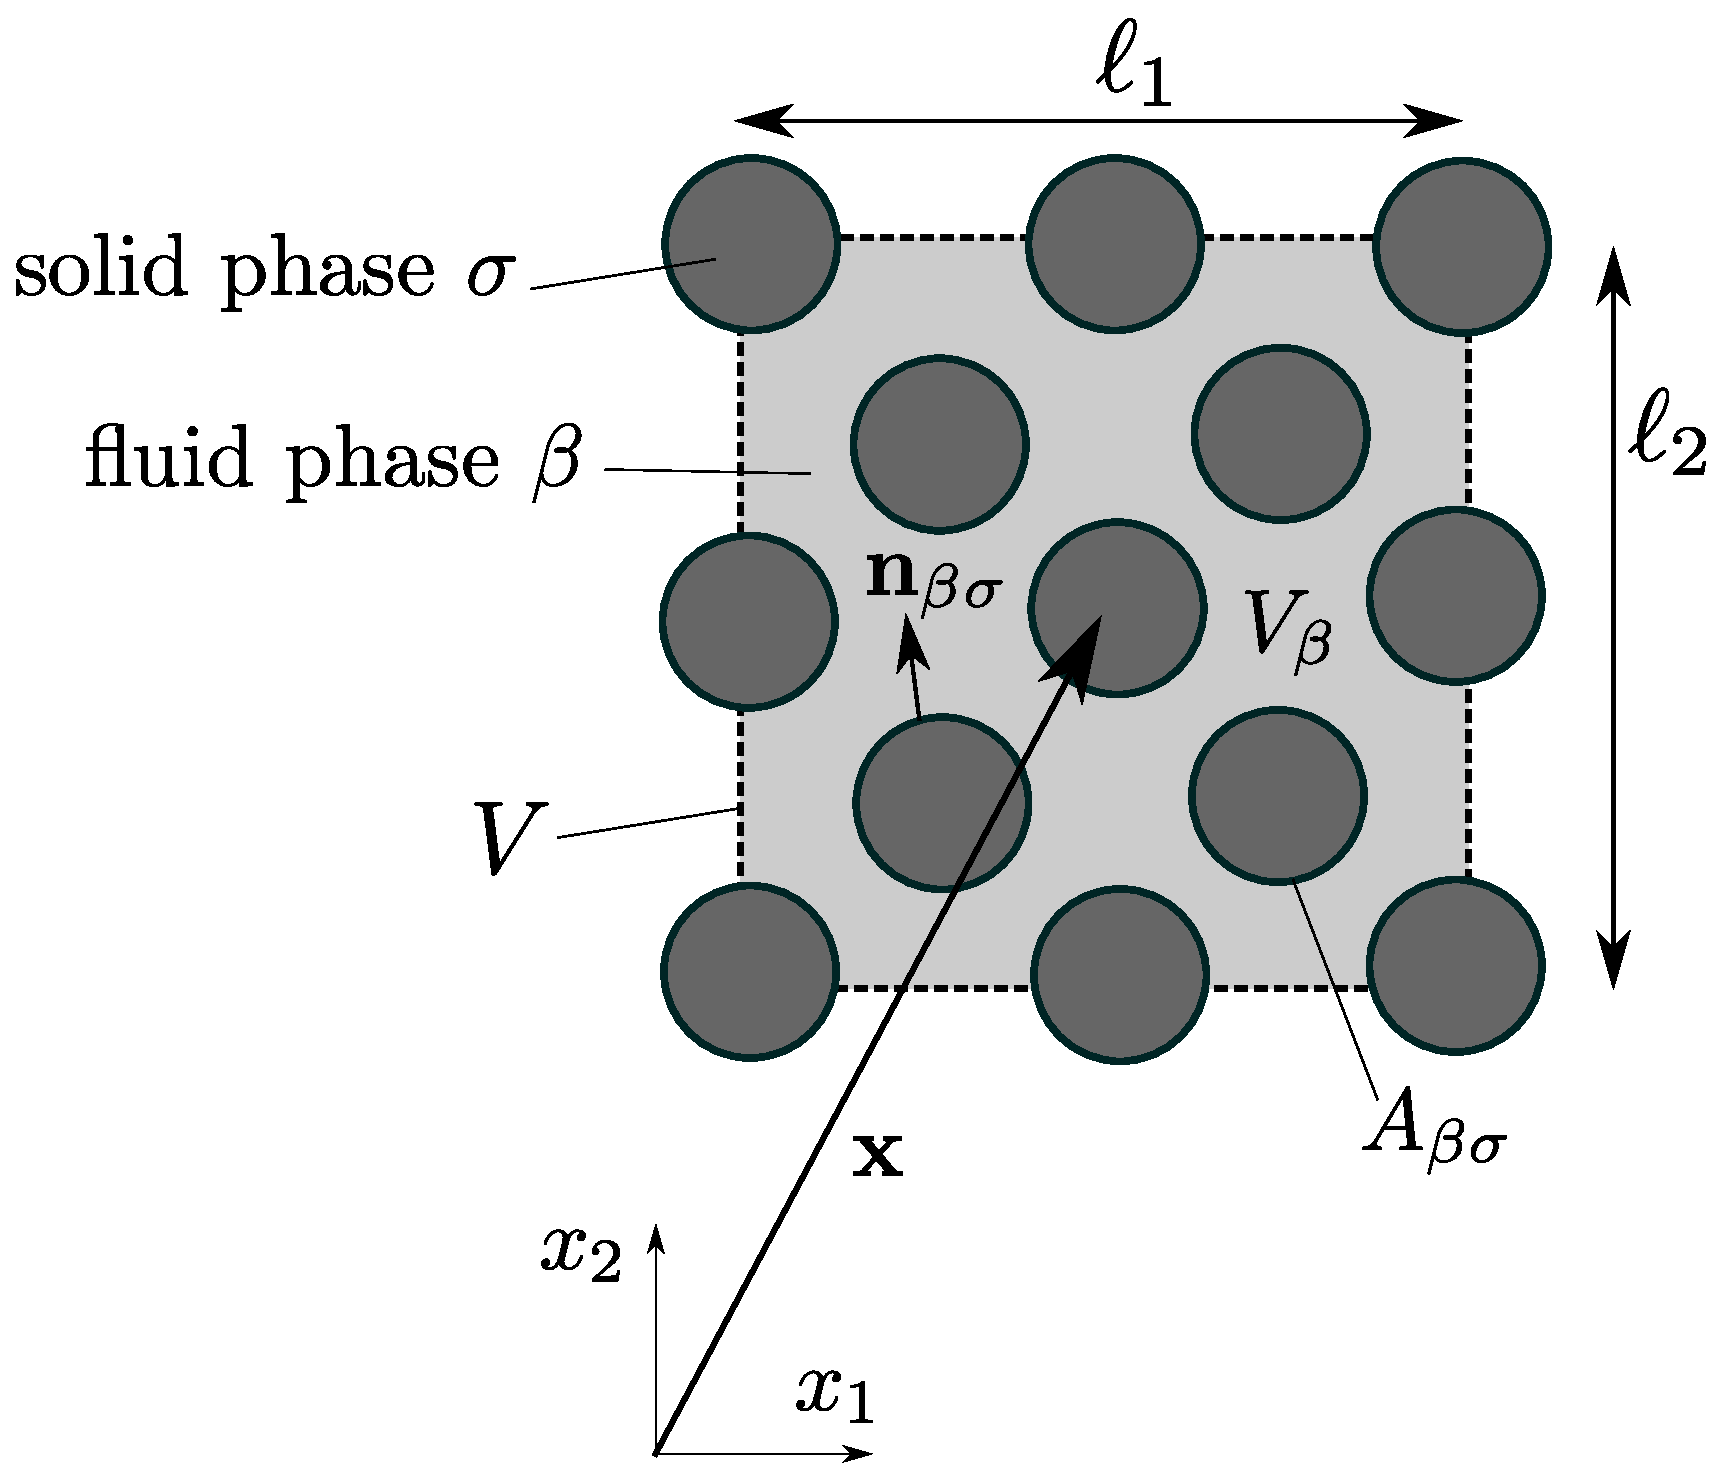
\includegraphics[width=0.8\linewidth]{chapter_4/figure/REV}
%	\caption{Illustration of the REV concept.}
%	\label{fig:rev}
%\end{figure}
%
%
%The concept of Reference Elementary Volume (REV) of the porous medium is classically introduced in the framework of the VANS approach.
%An example of REV  is depicted on figure \ref{fig:rev}, together with relevant notations (volume shape and size, indication of the fact that the normal unit vector is directed from the fluid to the solid phase, centroid $\rm {\bf{x}}$ of the REV). The REV represents  the domain over which the    microscopic problem is solved; its size is defined so as to contain all the microscopic features of the flow. 
%As a rule of thumb, the REV is the smallest  fluid domain over which   periodic boundary conditions can be applied.
%
%
%In the computational domain, any flow variable  $\phi$ can be decomposed into an intrinsic average part $\meani{\phi}$ plus a perturbation $\tilde{\phi}$, as:
%$$  \phi = \meani{\phi} + \tilde{\phi}.$$
%The intrinsic average is defined with an integration carried out only on the fluid phase \cite{whitaker2013method}:
%\begin{equation}
%\meani{\psi_{\beta}} = \dfrac{1}{\volb} \int_{\volb} \psi_\beta (\mathbf{x}) d \volb.
%\label{eq:avg_intrinsic}
%\end{equation}
%Applying such an operator to equations \eqref{eq:mom} and \eqref{eq:cont}, and following \citet{whitaker1996forchheimer} we have:
%$$
%\dfrac{\partial \vbmi}{\partial t} + \vbmi \cdot \nabla \vbmi = -\frac{1}{\rho_{\beta}} \nabla \pbmi + \nu_\beta \nabla^2 \vbmi + \, \mathbf{f} \, + 
%$$
%\begin{equation}
%\dfrac{1}{\volb} \int_{A_{\beta \sigma}}  ( - \frac{\pbt}{\rho_\beta} \mathbf{I} + \nub \nabla \vbt ) \cdot  \mathbf{n}_{\beta \sigma} dA,
%\label{eq:darcy_forch}
%\end{equation}	
%\begin{equation}
%\nabla \cdot \meani{\vb} = 0,
%\label{eq:cont_vans}
%\end{equation}	
%upon neglecting in equation \eqref{eq:darcy_forch} the sub-REV scale dispersion term (linked to the $\left< \vbt \vbt \right>^{\beta}$ term) which is often small in porous media flows \cite{brugem_phd}.
%
%The surface integral term in equation \eqref{eq:darcy_forch}  represents the drag (per unit mass) due to surface forces at the fluid-solid interface of the medium. It is called the Darcy-Forchheimer microscale force, $\mathbf{F}^{\textit{m}}$. The equations are however often to be solved at the macroscale, so that a macroscale force model, 
%$\mathbf{F}^{\textit{M}}$, must be used to replace $\mathbf{F}^{\textit{m}}$ in the governing equation. Such a model is often based on a permeability tensor, $\mathbf{K}$, and a Forchheimer tensor, $\mathbf{F}$, and reads:
%\begin{equation} 
%\mathbf{F}^{\textit{M}} = - \nub \mathbf{K}^{-1} (\mathbf{I} + \mathbf{F})\vbmi,
%\label{eq:macroscale} 
%\end{equation}
%so that the system is closed by imposing
%\begin{equation}
%\mathbf{F}^{\textit{m}} = \mathbf{F}^{\textit{M}}.
%\label{eq:closure_KF} 
%\end{equation}
%
%
%\noindent The drag force $\mathbf{F}^{\textit{m}}$ computed by direct numerical simulations (DNS) with account of all individual pores will be later compared to the model based on the permeability and Forchheimer tensors (whose equations are given below).
%This is just a useful exercise to demonstrate consistency of the approach and accuracy of the numerical simulations; it does nothing else since, as briefly described below, to derive the Forchheimer tensor the microscopic velocity field must be known anyhow.  Nonetheless, knowledge of the behaviour of these tensors (or, equivalently, of the related \emph{apparent} permeability) might prove both useful and instructive, in particular should one wish to extend the range of applicability of the model to cases for which the microscopic solution is not available.
%
%
%
%%%%%%%%%%%%%%%%%%%%%%%%%%%%%%%%%%%%%%%%%%%%%%%%%%%%%%%%%%%%%%
%%
%%\subsubsection{Closure problems for $\mathbf{K}$ and $\mathbf{F}$}
%%
%%%%%%%%%%%%%%%%%%%%%%%%%%%%%%%%%%%%%%%%%%%%%%%%%%%%%%%%%%%%%%
%
%
%The core of the VANS approach consists in the identification of the permeability and Forchheimer tensors. This problem, referred to as the closure problem, is discussed at length by \citet{whitaker1986flow,whitaker1996forchheimer}.  He derives two partial differential equation systems, the first valid in the zero Reynolds number limit (system \eqref{eq:K_closure} below), while the second applies when inertial terms are not negligible (system \eqref{eq:F_closure1}).
%
%
%
%In the first system of equations   a three component vector $\mathbf{d}$  and  a $3 \times 3$ tensor  $\mathbf{D}$ are introduced.
%This system  can be divided into  three separate independent problems which resemble a forced Stokes problem where each component of $\mathbf{d}$ and the corresponding row of  $\mathbf{D}$  play, respectively, the role of a pressure and a velocity field. Together with the periodic  boundary conditions, the problem reads: 
%\begin{equation}
%\begin{cases} 
%0 = -\nabla \mathbf{d} + \nabla^2 \mathbf{D} + \mathbf{I},\\ 
%\nabla \cdot \mathbf{D} = 0, \\ 
%\mathbf{D} = 0 \qquad {\rm on }  \qquad A_{\beta \sigma},\\
%\mathbf{d}(\mathbf{x} + \ell_i) = \mathbf{d}(\mathbf{x}), \qquad 
%\mathbf{D}(\mathbf{x} + \ell_i) = \mathbf{D}(\mathbf{x}) \qquad i = 1,2,3.
%\end{cases} 
%\label{eq:K_closure}
%\end{equation}
%The permeability tensor is found by applying  the intrinsic average on the $\mathbf{D}$ tensor, i.e.
%$\mathbf{K} = \varepsilon \; \meani{\mathbf{D}}$  and, in the Stokes regime, it is
%\begin{equation}
%\mathbf{F}^{\textit{M}} = - \nub \mathbf{K}^{-1} \vbmi.
%\end{equation}
%
%The second closure problem differs from the first only for the presence of a linearised convective term 
%in which the microscopic velocity obtained from the DNS, $\vb$, is used as an input.  This of course implies knowledge of the microscopic velocity field. A Oseen-like approximation which relaxes this constraint has been proposed by \citet{zampogna}.
%
%The new unknowns are a  vector and a tensor called, respectively,   $\mathbf{m}$  and  $\mathbf{M}$, with  the same meanings of $\mathbf{d}$ and 
%$\mathbf{D}$.
%The system reads:
%\begin{equation}
%\begin{cases} 
%\dfrac{1}{\nub} \vb \cdot \nabla \mathbf{M} = -\nabla \mathbf{m} + \nabla^2 \mathbf{M} + \mathbf{I},\\ 
%\nabla \cdot \mathbf{M} = 0, \\ 
%\mathbf{M} = 0  \qquad {\rm on } \qquad A_{\beta \sigma}, \\
%\mathbf{m}(\mathbf{x} + \ell_i) = \mathbf{m}(\mathbf{x}), \qquad 
%\mathbf{M}(\mathbf{x} + \ell_i) = \mathbf{M}(\mathbf{x}) \qquad i = 1,2,3.
%\end{cases} 
%\label{eq:F_closure1}
%\end{equation}
%The average  of the tensor $\mathbf{M}$  multiplied by the porosity is the \textit{apparent permeability}, 
%$\mathbf{H}= \varepsilon \; \meani{\mathbf{M}}$. When inertia is important equation \eqref{eq:macroscale}  can be written as 
%\begin{equation}
%\mathbf{F}^{\textit{M}} = - \nub \mathbf{H}^{-1} \vbmi,
%\end{equation}
%\noindent as shown by \citet{whitaker1996forchheimer}.
%
%Two remarks are in order at this point.
%First, the equations in the closure problem \eqref{eq:F_closure1} are time-independent because the microscopic velocity $\vb$ is a solution of a stationary DNS.  Thus, the Reynolds number should be sufficiently small for unsteady effects not to be present. Should the wake behind a solid inclusion display regular or irregular temporal oscillations, the equations of system \eqref{eq:F_closure1} may be used, as an
%approximation, by replacing the instantaneous velocity in the REV with its time-averaged distribution.  This case is however not of present concern.
%Secondly, the closure problems reflect the structure of the solution of the two system \eqref{eq:K_closure} and \eqref{eq:F_closure1}. In particular, the solution of \eqref{eq:K_closure} depends only on the geometry of the porous medium so that the permeability tensor $\mathbf{K}$ is symmetric. This is not the case for $\mathbf{H}$, because of the effect of the microscopic velocity amplitude and direction.  Clearly, the solution of system \eqref{eq:K_closure} tends to that of \eqref{eq:F_closure1} when $Re_d \rightarrow 0$. 
%



%%%%%%%%%%%%%%%%%%%%%%%%%%%%%%%%%%%%%%%%%%%%%%%%%%%%%%%%%%%%%%

\section{Validation and setup }

%%%%%%%%%%%%%%%%%%%%%%%%%%%%%%%%%%%%%%%%%%%%%%%%%%%%%%%%%%%%%%%


In this section the numerical methodology, the parameters, the setup and the validation for some reference cases are given.


%%%%%%%%%%%%%%%%%%%%%%%%%%%%%%%%%%%%%%%%%%%%%

\subsection{Computational domain}

%%%%%%%%%%%%%%%%%%%%%%%%%%%%%%%%%%%%%%%%%%%%%


The geometry used for the base REV is shown in figure \ref{fig:cell_3d}: a cylindrical inclusion is present at the centre of the REV and four quarters of cylinders are situated at the corners. The lateral length of the cubic envelop is $\ell$, which is used as length scale for the microscopic problem; the diameter $d$ of the cylinders is adapted as a function of the desired porosity $\varepsilon$, ratio between the fluid volume over the total REV volume ($\ell^3$). 

The  forcing term $\mathbf{f}$ of the DNS  is a vector whose direction is defined by two Euler angles, with rotations of the form:  $\theta \ \mathbf{e_3} + \phi \ \mathbf{e_2}^{I}$ (cf. figure \ref{fig:cell_3d}). Its amplitude is set a priori and is connected to the Reynolds number, $Re_d$, defined with the mean velocity over the REV and the fiber diameter, $d$. $Re_d$ is a result of the calculations, once the mean velocity is evaluated.

\begin{figure}[h]
	\centering
	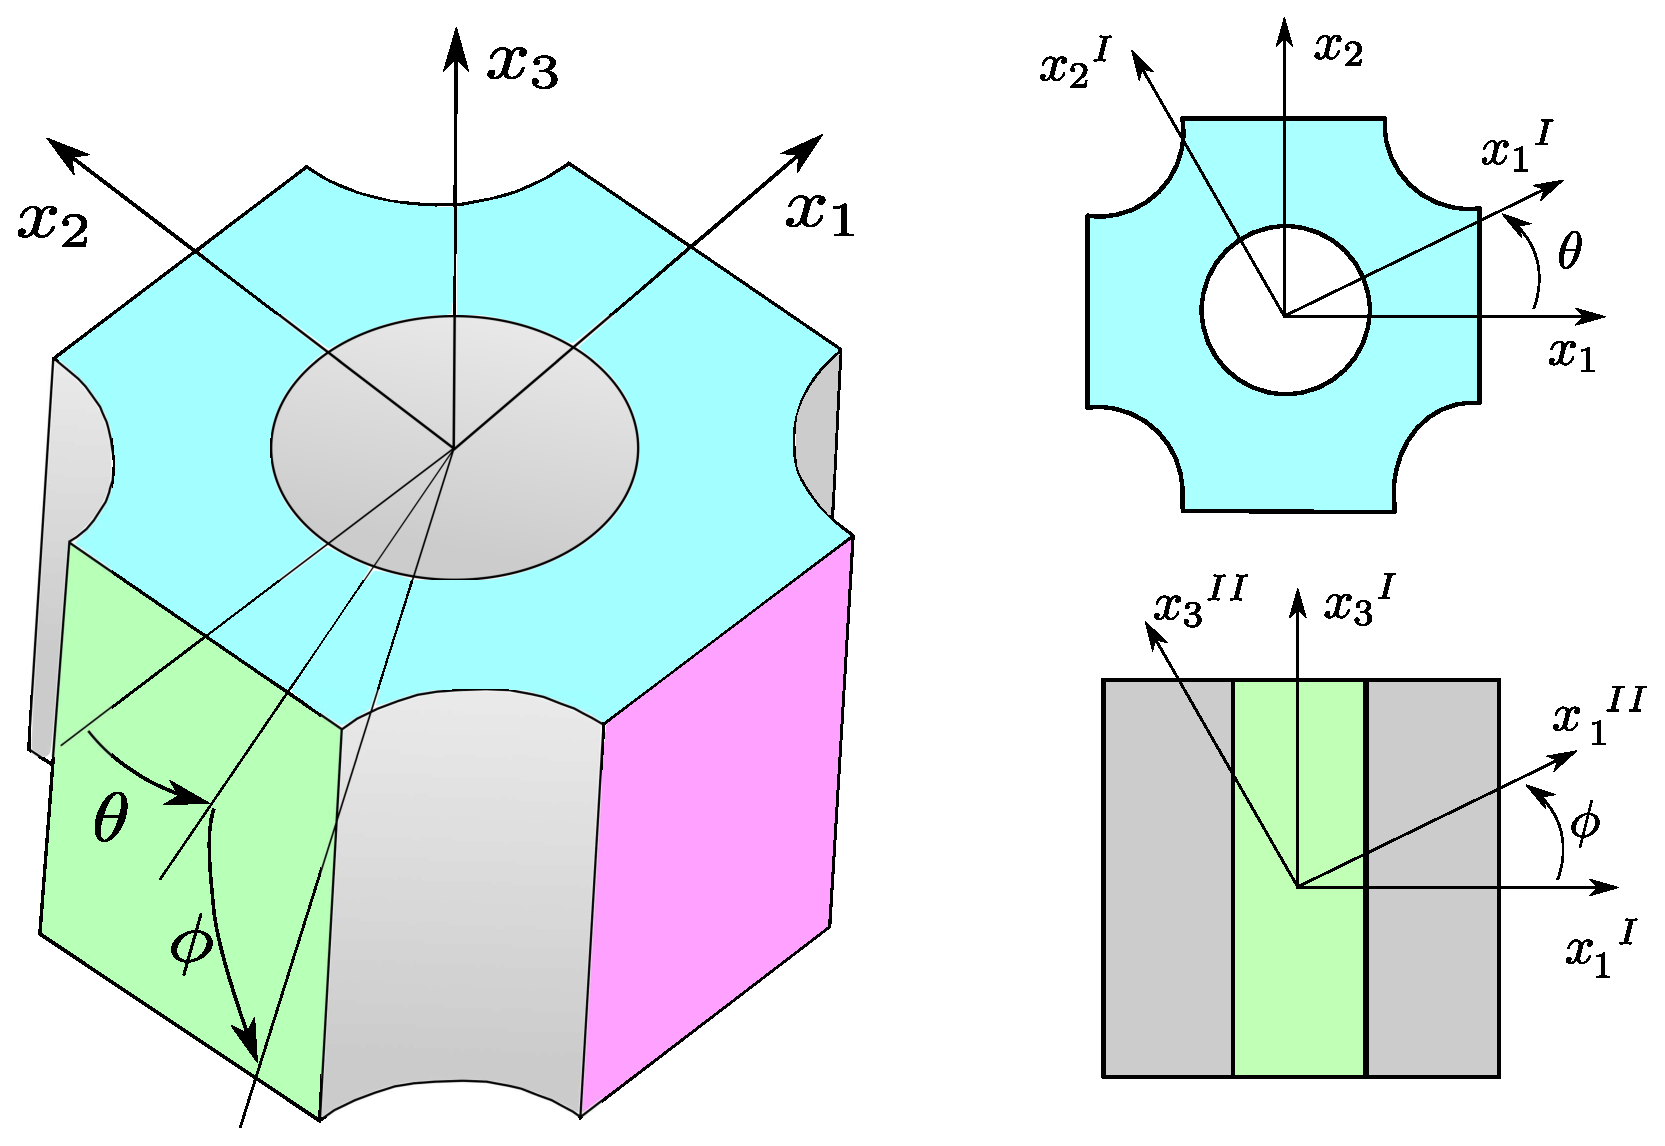
\includegraphics[width=0.8\linewidth]{chapter_4/figure/cell_3d}
	\caption{REV for the fiber geometry investigated.}
	\label{fig:cell_3d}
\end{figure}


%%%%%%%%%%%%%%%%%%%%%%%%%%%%

\subsection{Numerical setup}
\label{ph:numeric_setup}

%%%%%%%%%%%%%%%%%%%%%%%%%%%%


The simulations have been carried out with the open-source code OpenFOAM \cite{openfoam}, based on  a finite volume discretization with a colocated arrangement for the unknowns.
The standard solver icoFoam (incompressible Navier-Stokes) has been modified in order to include a constant pressure gradient acting as a forcing term $\mathbf{f}$  in equation \eqref{eq:mom}. 
The coupling between  the velocity and the pressure equations is based on the pressure implicit split operator referred to as the PISO algorithm. 
The time derivative term is discretized using the second order backward Euler scheme and all the spatial terms use a second-order central difference stencil  based on Gauss finite volume approach. The velocity system is solved with a preconditioned bi-conjugate gradient (PBiCG) iterative solver with the tolerance on the velocity residuals set to $10^{-8}$, associated to a   diagonal incomplete lower upper pre-conditioner (DILU).
The pressure equation is solved with a  geometric-algebraic multigrid  (GAMG) algorithm associated to a Gauss-Seidel smoother and the tolerance on the pressure residuals is here equal to $10^{-6}$.  Cyclic boundary conditions are applied to all fields on all fluid
boundaries along the three directions, and the no-slip condition is imposed on the surface of the solid inclusions. 
The time step $\Delta t$  is automatically determined to ensure  that the maximum Courant number, $Co$, respects the condition:
$Co =  ||v_\beta||  \ \Delta t / \Delta x < 1/2 $, in which $||v_\beta||$ is the local velocity magnitude in the REV and $\Delta x$ is the local grid spacing. $Co$ 
is basically the ratio between the fluid speed  and the velocity to propagate information through the mesh and the condition $Co < 1/2$ is found to be sufficient to have a stable solver.



%%%%%%%%%%%%%%%%%%%%%%%%%%%%%%%%%%%%%%%%

\subsection{Mesh convergence analysis }

%%%%%%%%%%%%%%%%%%%%%%%%%%%%%%%%%%%%%%%%


The mesh has been computed using  the internal OpenFOAM mesher named \textit{snappyHexMesh}.
The final grid is mainly composed by hexahedral cells with a refined regular grid in the boundary layer regions next to the solid surfaces.
Three different mesh sizes, with $0.65 \times 10^6$, $10^6$ and $1.5 \times 10^6$ elements, have been tested in order to demonstrate spatial convergence. This has been assessed using the Grid Convergence Index ($GCI$) introduced by \citet{roache}.



Details of the coarsest mesh used are shown in figure \ref{fig:mesh1}. On the  right frame a close up of the grid in the neighbourhood of the fiber's boundary is displayed: twenty points are used in the structured portion of the mesh along the wall-normal direction.



\begin{figure}[h]
	\centering
	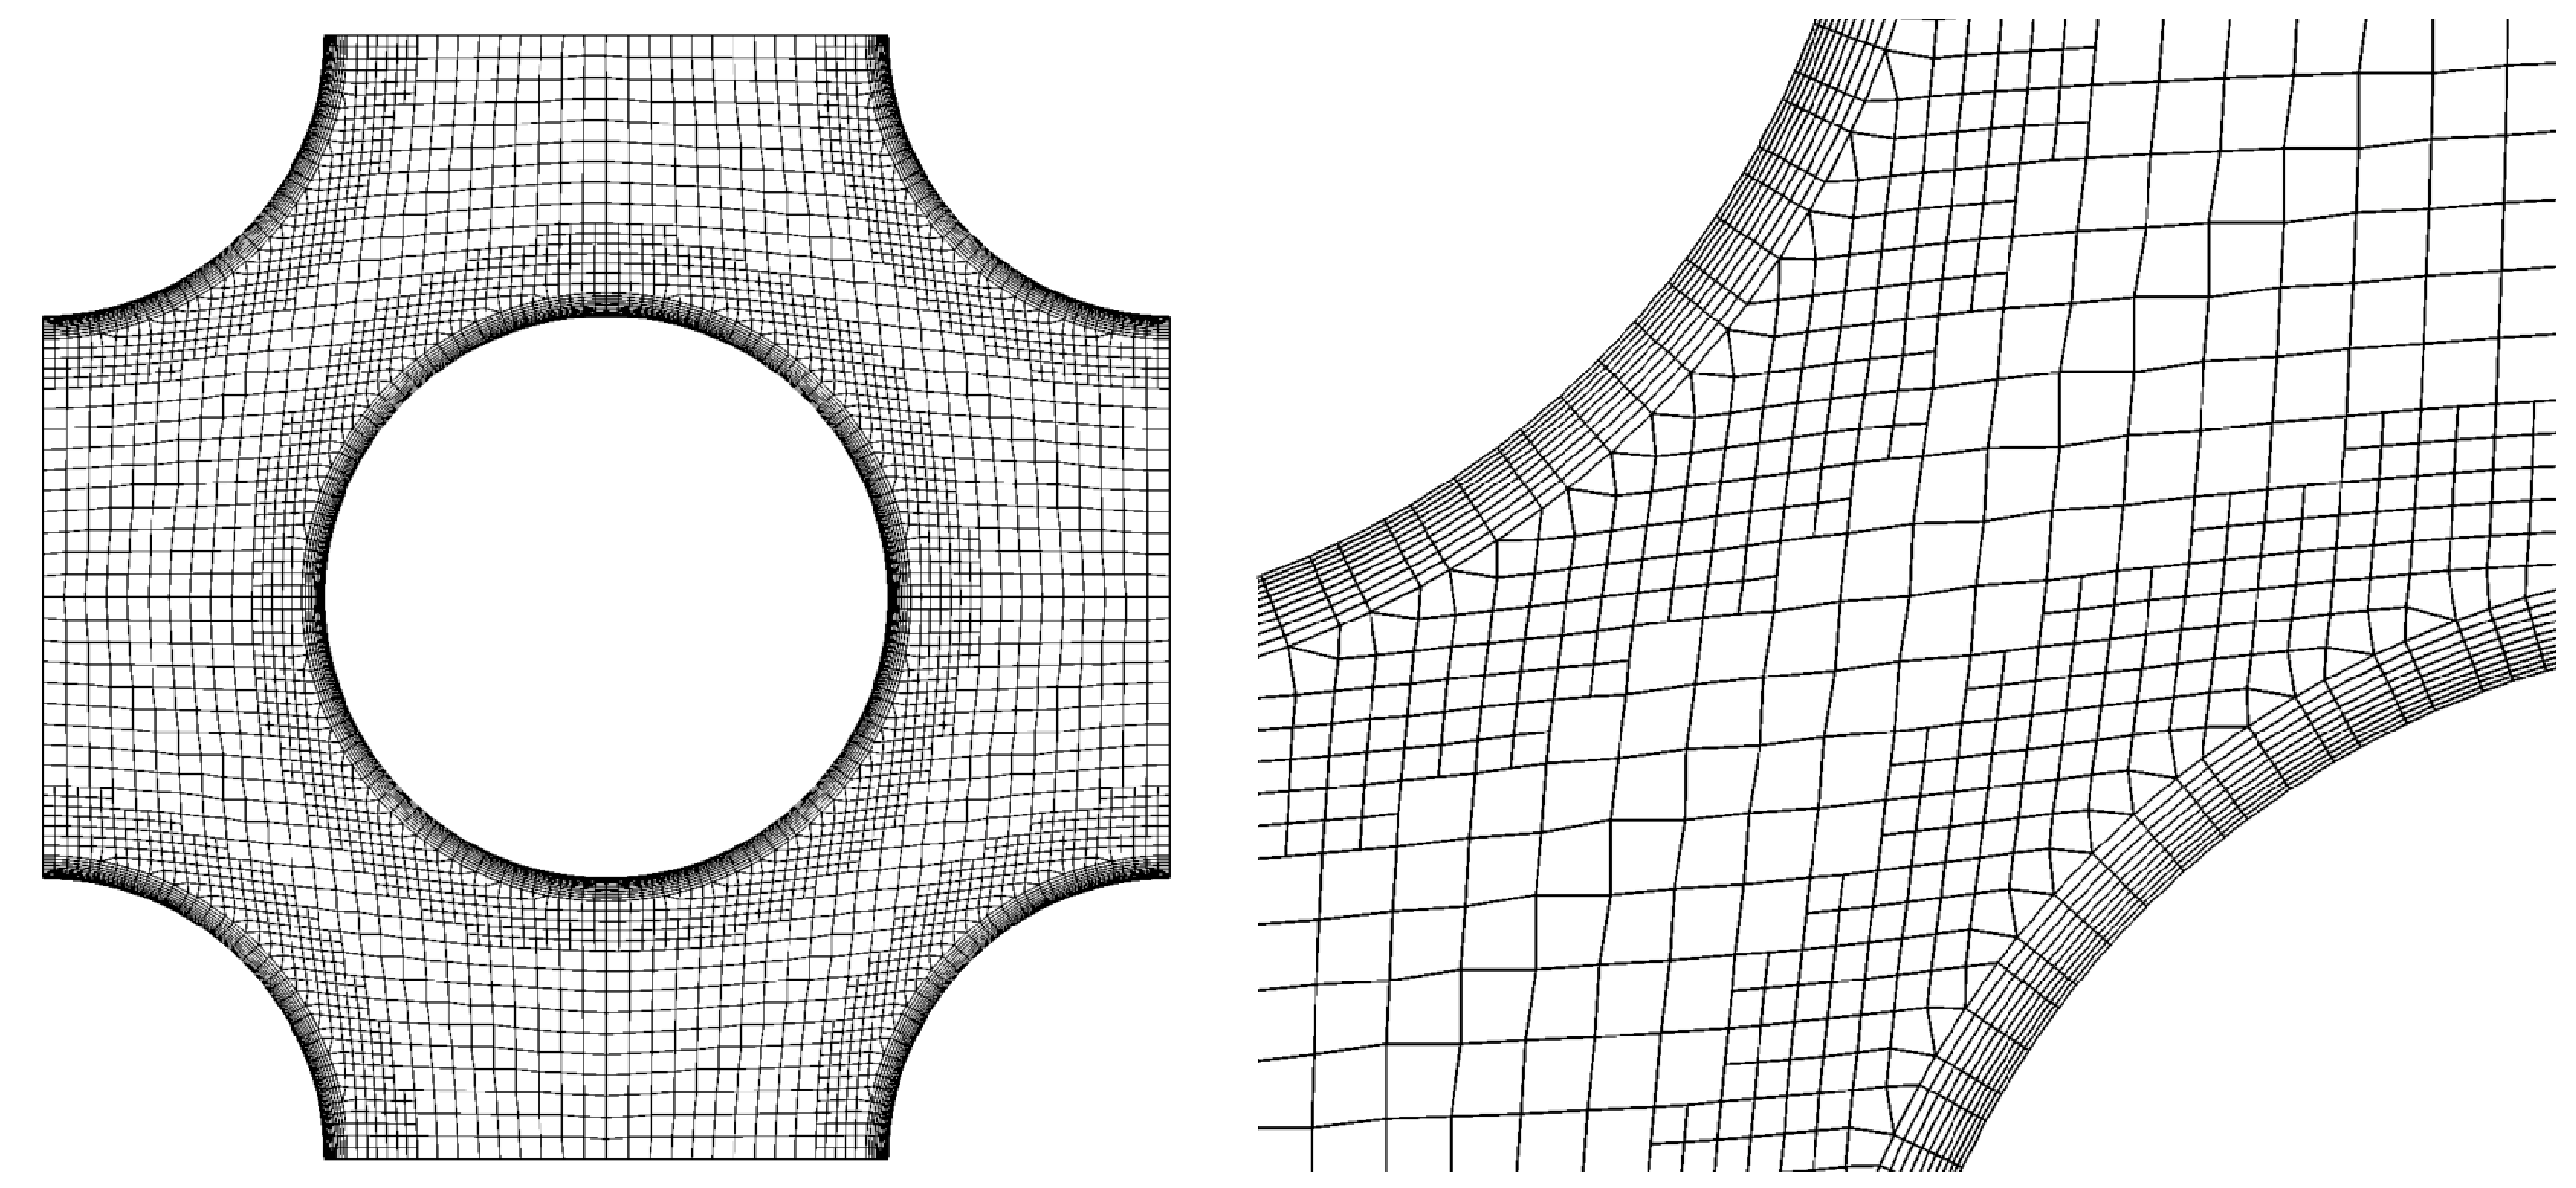
\includegraphics[width=0.8\linewidth]{chapter_4/figure/mesh}
	\caption{Mesh used for the computation; top view (left) and zoom in the boundary layer region (right). $\varepsilon = 0.6$.}
	\label{fig:mesh1}
\end{figure}




The GCI method is based upon a grid refinement error estimator derived from the
theory of generalized Richardson extrapolation. It measures the ratio between the computed value of a quantity over the asymptotic numerical value, thus indicating how far the solution is from the asymptotic ("exact") value.
The procedure is simple and provides a method to estimate the order of the spatial
convergence, based on two or three different grid sizes.
First of all, the grids must be generated with the same algorithm and they must  have the same final quality.
In each simulation   a physical scalar quantity representative of the physical phenomenon must be sampled.
The method follows the following four steps:

\begin{enumerate}
	\item  Estimate the order of convergence of the procedure, defined as
	$p = \ln \rprth{\dfrac{f_3 - f_2}{f_2 - f_1}}   / \ln r $,
	where $r$ is the grid refinement ratio between each grid (it is computed as the ratio between the number of elements of two consecutive grids; the approach imposes that $r$ should remain constant between any couple of consecutive grids and be larger than $1.1$), and $f_i$
	represents the quantity of interest in each grid (1=coarse, 2=medium and
	3=fine).
	
	
	\item Compute the relative error between grid $i$ and $j$:
	${|\epsilon|}_{ij} = \dfrac{f_j - f_i}{f_i}$, for $(i,j)$
	$\in \left\{ (1,2), (2,3) \right\}$.
	
	\item Compute
	$ {GCI}_{ij}=\dfrac{F_s {|\epsilon|}_{ij}}{r^p -1}$, with
	$F_s$ a safety factor equal to 1.25 if the grids are three, and equal to 3 if the grids are only two \cite{roache}.
	
	\item Check whether each grid level yields a solution that is in the asymptotic range of convergence; this means that the quotient
	$ AC = \dfrac{{GCI}_{23}}{{GCI}_{12}} \dfrac{1}{r^p}$ should be as close as possible to one.
\end{enumerate}


\noindent In our case the quantity of interest chosen is the intrinsic average velocity inside the porous medium, and the results are summarized in table \ref{table:convergence}.
\begin{table}[t]
	\begin{center}
		\begin{tabular}{ l  |l   l   }
			\vspace{-0.3cm}
			mesh   &	mesh   & average REV  \\
			index  &	identifier  &  velocity \\ 
			\hline \hline
			3 &	fine & 1.11  \\ 
			2 &	medium & 1.07  \\ 
			1 & coarse & 1.09  \\ 
			\hline
		\end{tabular}
		$\qquad$
		\begin{tabular}{ l | l   }\vspace{0.35cm} 
			metric & value \\ \hline \hline
			${GCI}_{23}$ & 0.366\%  \\ 
			${GCI}_{12}$ & 1.11\%  \\ 
			AC & 1.006  \\
			\hline
		\end{tabular}
		\caption{Convergence analysis. Left: average velocity within the REV, normalized with $\displaystyle{\frac{K_{11}}{\nu_{\beta}} ||\bf{f}||}$. 
			Right: grid convergence metrics. The REV has $\varepsilon=0.6$, the motion is along $x_1$, i.e. 
			$\theta=\phi=0$ and $Re_d \rightarrow 0$.}
		\label{table:convergence}
	\end{center}
\end{table}
From the table it can be seen that the intrinsic velocity difference is very small from one grid to the next and the coarse grid provides results close to the expected asymptotic value. This is taken as a sufficiently convincing argument to carry out all the computations in the following with a grid density equal to that of grid 1. 



%%%%%%%%%%%%%%%%%%%%%%%%%%%%%%%%%%%%%%%%%%%%%%%%%%%%%%%
\subsection{Validation on two different configurations}
%%%%%%%%%%%%%%%%%%%%%%%%%%%%%%%%%%%%%%%%%%%%%%%%%%%%%%

The results published in the literature by \citet{zampogna} and \citet{yazdchi2011} are now used to validate both the methodology and our choices of the computational parameters. In the cited papers, three-dimensional  computations of the permeability components in different cells geometries are presented.

Figure \ref{fig:square} displays the comparison for a cell with a square arrangements  of the fibers; here the permeability is evaluated along the two principal directions, $x_1$ and $x_3$.
%The present computation are plot with triangles for the two $K_{11}$ and $K_{33}$ components.
A good agreement is found with the published results. 
%For permeability $\varepsilon$ larger than $0.85$, some small discrepancies can be seen but it is at the limit of the theory.
%The trends are well captured as well by comparison with the empirical fitted solution given by the reference.
\begin{figure}[t]
	\centering
	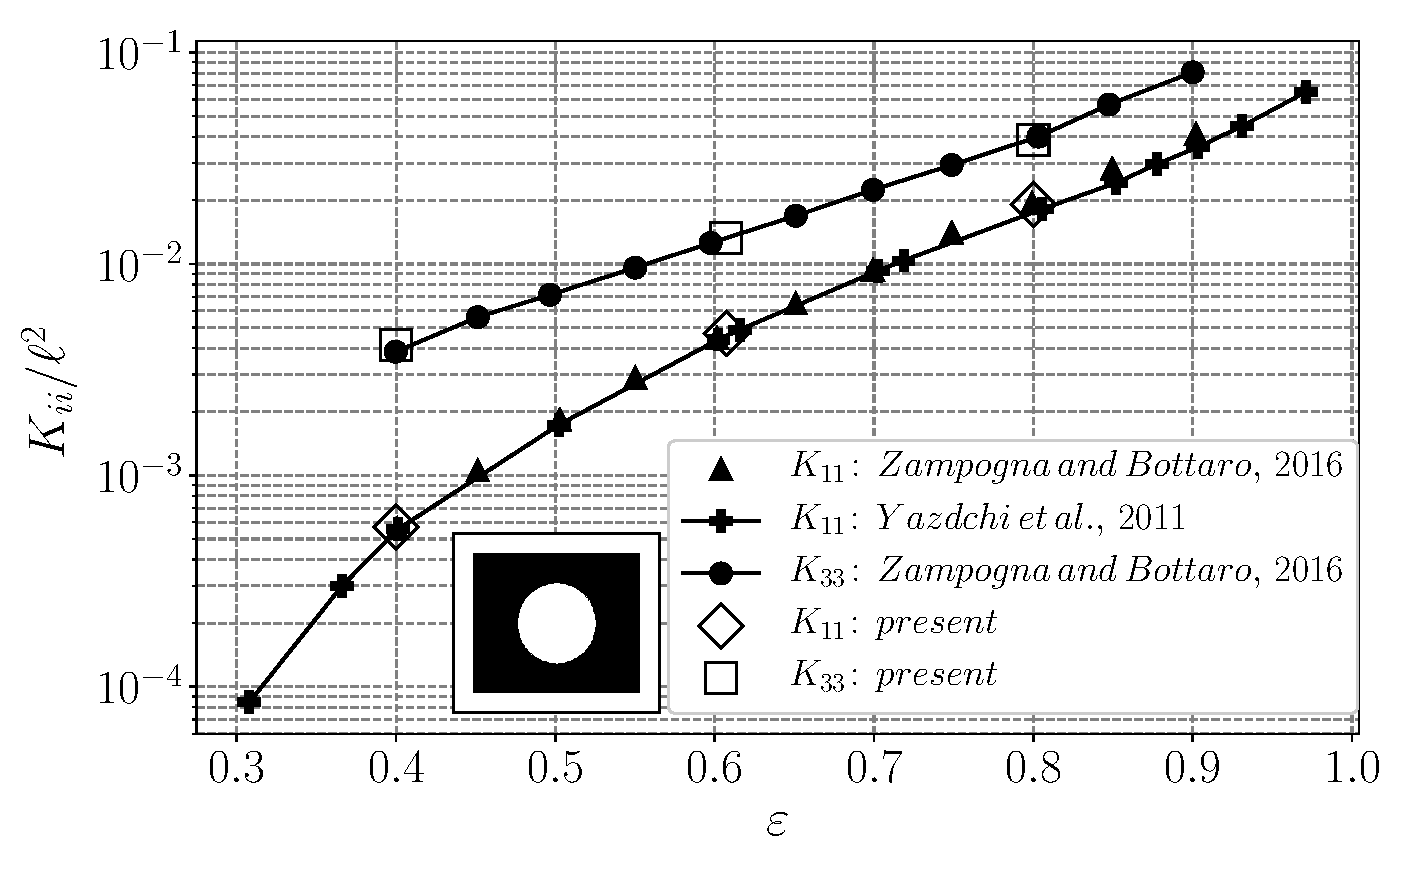
\includegraphics[width=0.8\linewidth]{chapter_4/figure/square}
	\caption{Permeability versus porosity for a square arrangement of cylinders. The scaling of the permeability is $\ell^2$ and is explicitely indicated in the vertical axis.}
	\label{fig:square}
\end{figure}
Figure \ref{fig:hexa} shows a similar comparison for a staggered arrangement of the inclusions in the unit cell. In this case the section of the cell is rectangular. The agreement for the only permeability component available in the literature is again satisfactory.
\begin{figure}[h]
	\centering
	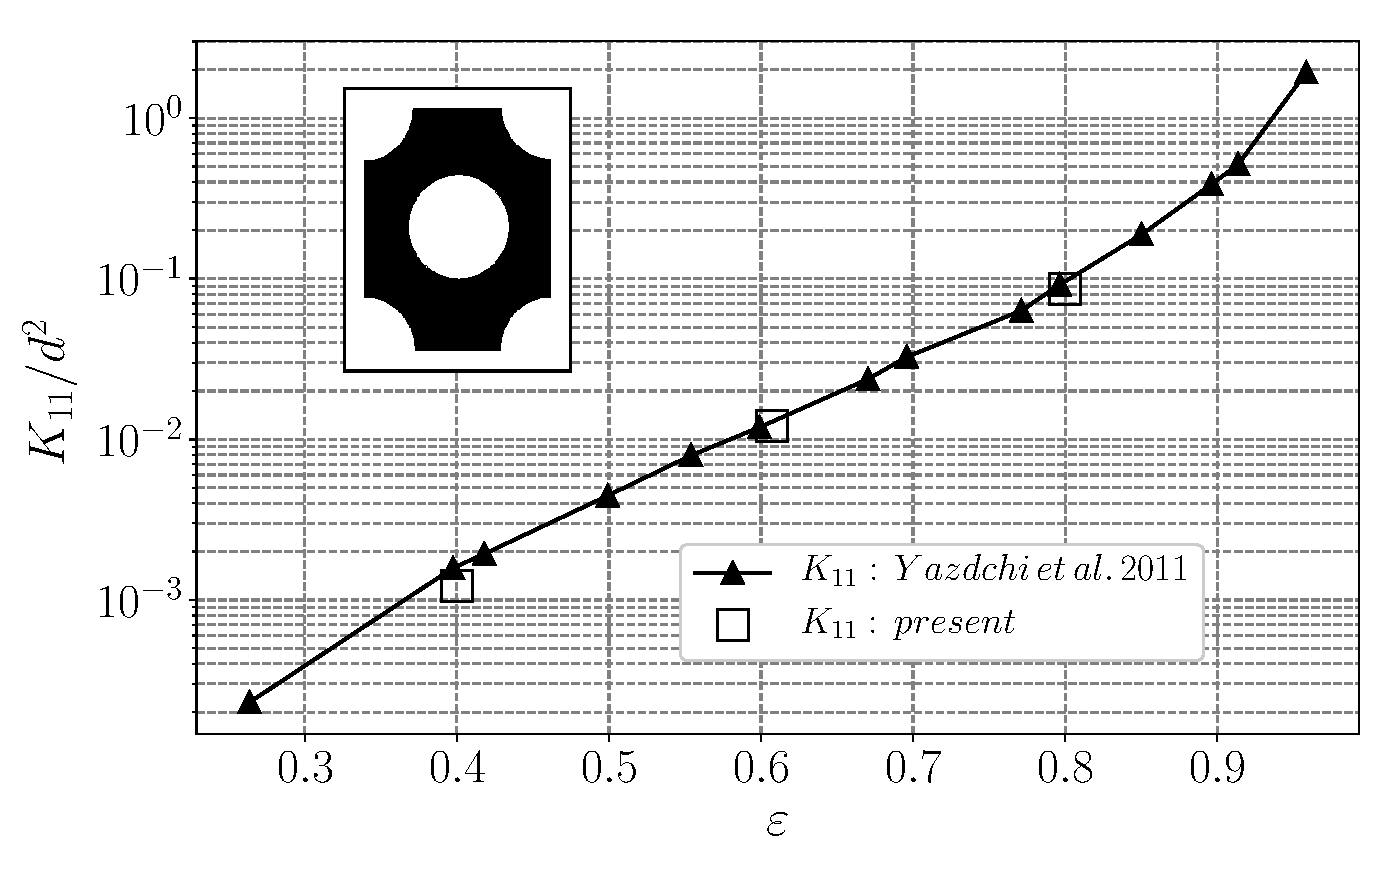
\includegraphics[width=0.8\linewidth]{chapter_4/figure/hexa}
	\caption{Permeability versus porosity for a staggered arrangement of cylinders. The permeability component is here scaled with $d^2$ (and not $\ell^2$), with $d$ the diameter of the inclusions.}
	\label{fig:hexa}
\end{figure}

\begin{figure}[h!]
	\centering
	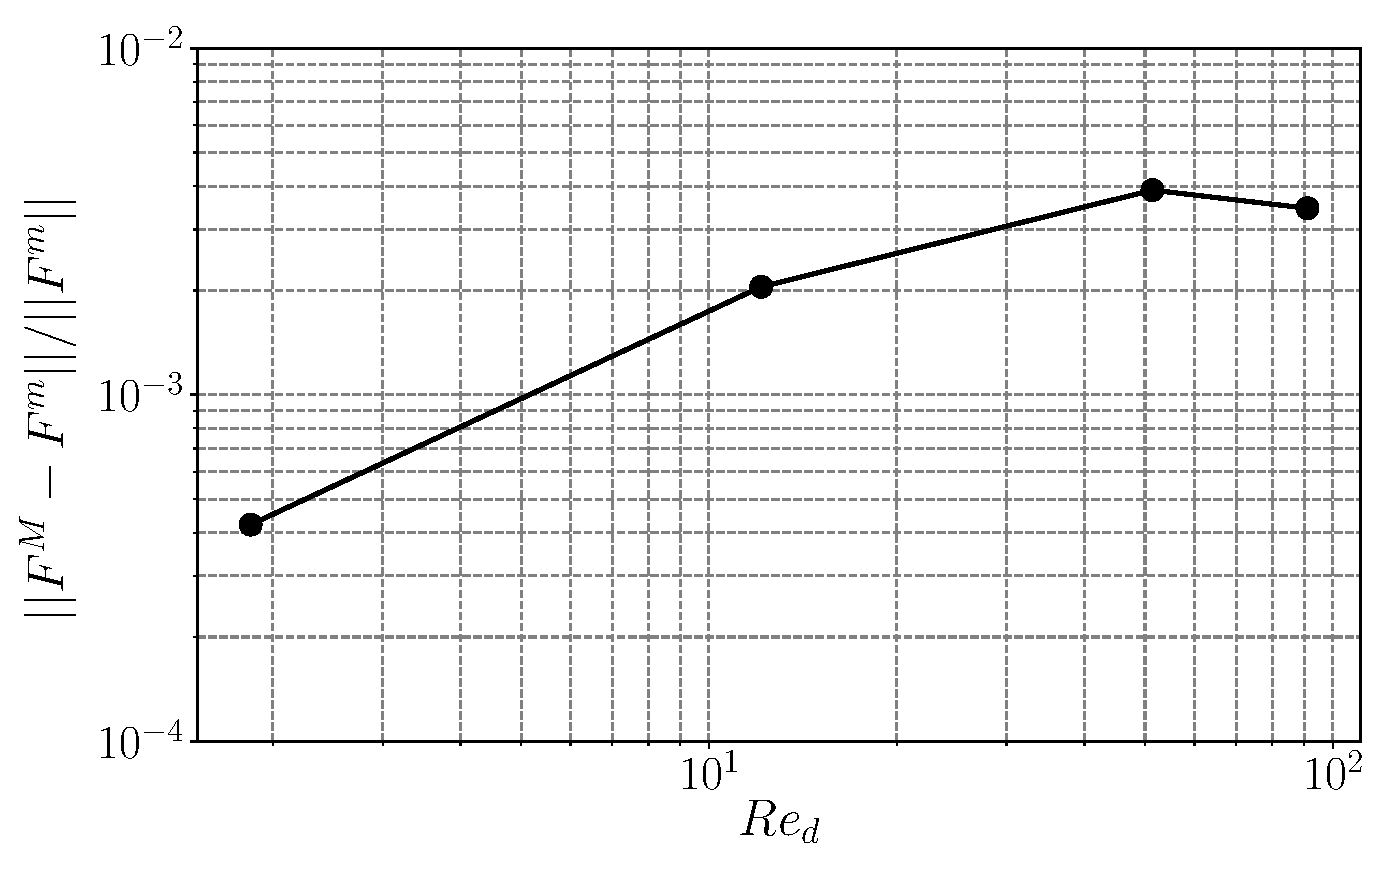
\includegraphics[width=0.8\linewidth]{chapter_4/figure/macro_force}
	\caption{Relative error between the microscopically computed forces along the $x_1$ direction and those arising from the Darcy-Forcheimmer model; $\varepsilon=0.8$ for the REV in the staggered arrangement of \citet{yazdchi2011}.}
	\label{fig:force_comparison}
\end{figure}	
Finally, to check the correct implementation of the closure model \eqref{eq:closure_KF} it is important to verify the equality \eqref{eq:closure_KF}  between the amplitude $F^M$ of the macroscopic force and its microscopic counterpart obtained through an integration of the DNS fields over the solid boundaries of the inclusions in the REV. Figure \ref{fig:force_comparison} shows a plot of the relative error between these two forces, i.e. 
$\displaystyle \frac{||F^M-F^m||}{||F^m||}$, as function of the Reynolds number. We consider the successful comparison displayed in figure \ref{fig:force_comparison} 
as the conclusive demonstration of the validity of the approach described here. We have nonetheless carried out the same verification displayed in figure \ref{fig:force_comparison} for each one of the simulations described in the following, to our satisfaction.



%%%%%%%%%%%%%%%%%%%%%%%%%%%%%%%%%%%%%%%
\subsection{Tests with larger REV's}
%%%%%%%%%%%%%%%%%%%%%%%%%%%%%%%%%%%%%%%

Since the Reference Elementary Volume (REV) is the unit cell within the porous medium over which average quantities of the VANS are computed, 
it is important to choose its dimensions appropriately in the inertial regime for, if the REV is too small, it might be easy to miss crucial 
features of the wakes. For example, to predict the  critical Reynolds number, $Re_c$, of the first Hopf bifurcation, a REV containing at least 
three solid inclusions in the direction of the mean pressure gradient is necessary in the simulations by \citet{lasseux_hopf}. Among the 
results 
reported, it is found that, for a fixed REV size, the error committed in the evaluation of the critical Reynolds number increases with the 
porosity. This same error is considerably reduced when the mean pressure gradient angle is $\theta=45^\circ$. Thus, the choice of the number of 
inclusions in a REV is a task not to be overlooked, and the final choice must account for the porosity, the direction of the pressure gradient 
and the microscopic Reynolds number.

Here, the influence of the numbers of inclusions present in a REV is assessed by focussing only on the velocity components after averaging over the REV. The unit cubic cell of side $\ell$ is used as reference: starting from this, two additional REV's are built, as shown in figure \ref{fig:multiple}. The first one is doubled in both the $x_1$ and $x_2$ directions and the case tested numerically is characterised by $\theta=0$, $\phi=0$ (i.e. the forcing pressure gradient is directed along $x_1$), porosity $\varepsilon=0.6$ and $Re_d=50$. 
The second REV configuration is a composition of 3 reference REVs on top of one another along $x_3$, with the parameters set to $\theta=45^\circ$, $\phi=45^\circ$,  $\varepsilon=0.6$ and $Re_d=100$.

For both these test cases, no appreciable differences, neither in the mean velocity nor in the forces on the fibers, have been observed, with relative errors on the mean velocity with respect to the reference case which remain below  2\%.  We take this as sufficient evidence to use, in the following, only the reference cubic REV of side equal to $\ell$, with the understanding that only configurations with $Re_d$ up to around 100 can be considered.

\begin{figure}[h!]
	\centering
	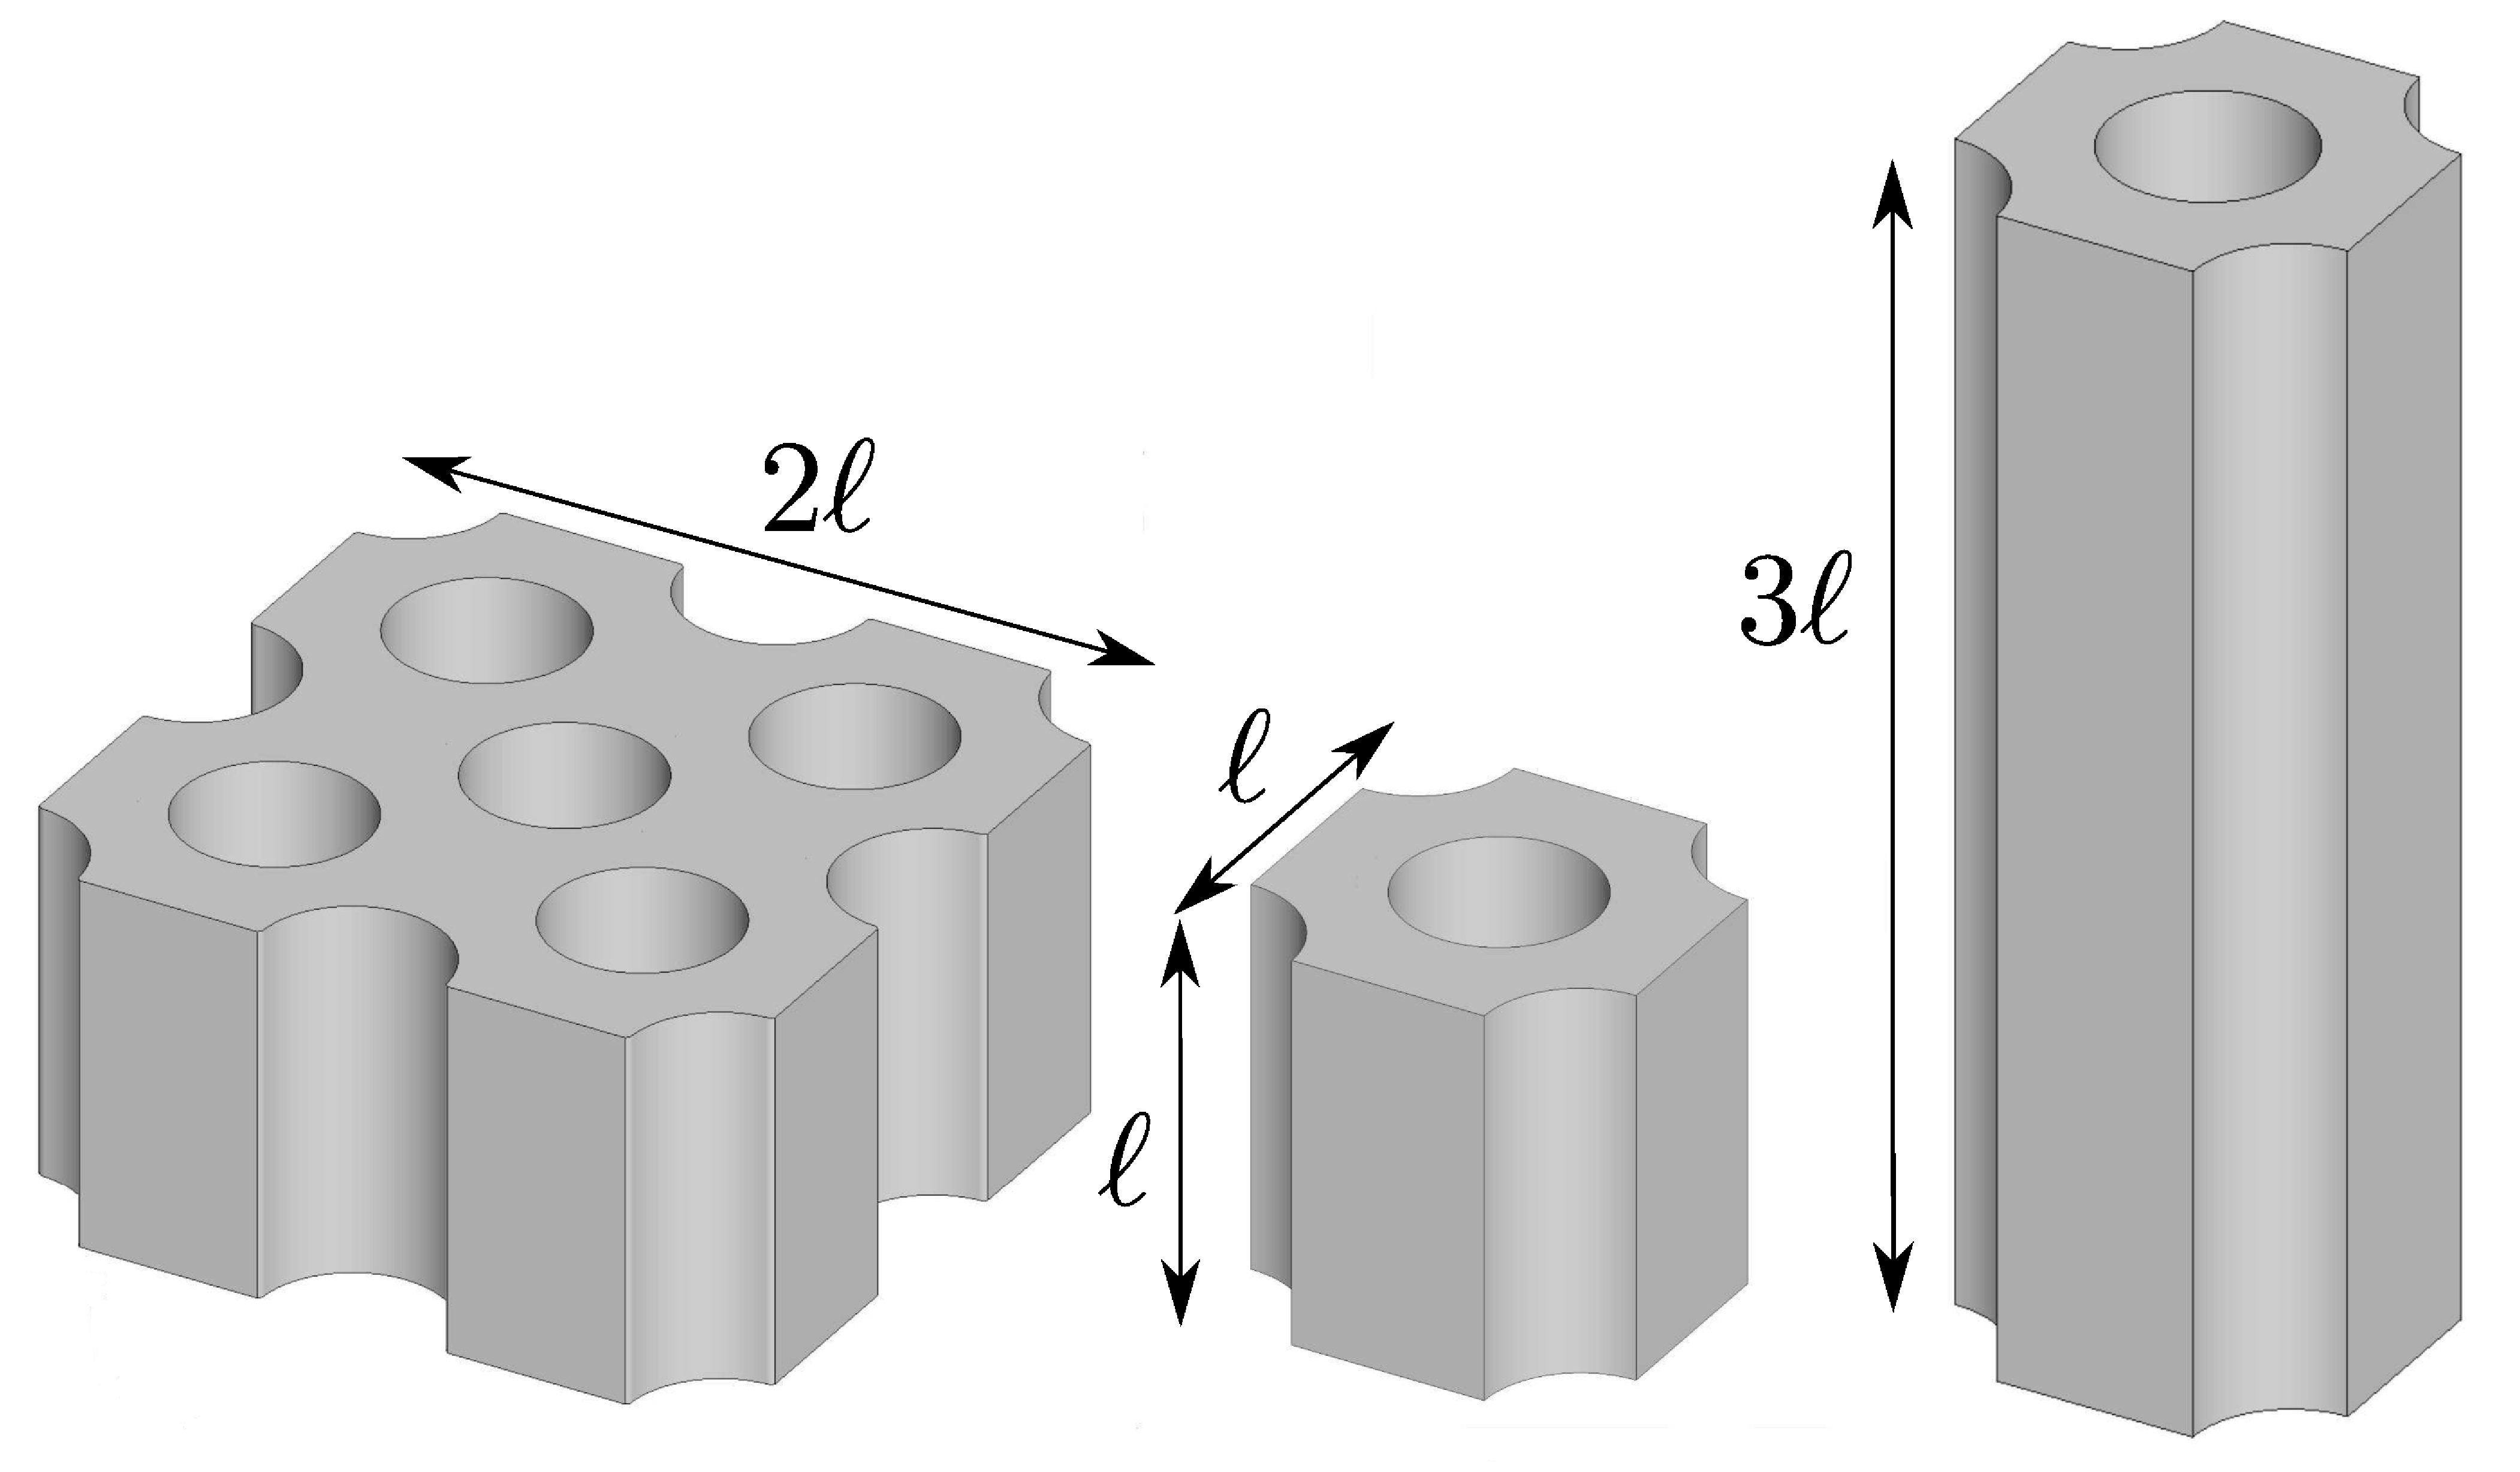
\includegraphics[width=0.8\textwidth]{chapter_4/figure/multiple}
	\caption{REV configurations. Left: $2 \times 2 \times 1$ arrangement; centre: $1 \times 1 \times 1$ arrangement (reference);  right $1 \times 1 \times 3$ arrangement.}
	\label{fig:multiple}
\end{figure}



%%%%%%%%%%%%%%%%%%%%%%%%%%%%%%%%%%%%%%%%%%%%%%%%%%%
\section{Microscopic solutions}
%%%%%%%%%%%%%%%%%%%%%%%%%%%%%%%%%%%%%%%%%%%%%%%%%%

In this section, some local microscopic fields computed with direct numerical simulations are shown, together with components of the intermediate tensor $\mathbf{M}$ coming from the numerical solution of the closure equations \eqref{eq:F_closure1}. 

In figure \ref{fig:1ch4} (top row) the local $x_1$ velocity component is drawn for the two-dimensional flow when $\varepsilon=0.6$, for three 
Reynolds numbers, to cover the transition from the Stokes to the inertial regime. In all plots, the velocities are rendered non-dimensional by
the corresponding value of 
$\displaystyle{\frac{K_{11}}{\nu_{\beta}} ||\bf{f}||}$. When inertia is absent, the flow has a central symmetry; by increasing the Reynolds number, only the 
symmetry with respect to the $x_1$ axis is maintained ($x_1$ is the direction of the forcing pressure gradient), with the wake's length which 
increases with $Re_d$. When $Re_d$ is of order 100 the wake spreads to the downstream boundary of the REV, re-entering, because of periodicity, 
at the upstream side.	This $Re_d$  represents the upper limit of validity for the cubic unit cell of side $\ell$; larger values of $Re_d$ 
could only be investigated with longer/larger/thicker REV's.

The non-dimensional local $M_{11}$ fields for the same parameters are displayed in figure \ref{fig:1ch4} (mid row). All values in the figures 
arise from scaling $\bf{M}$ with $\ell^2$. Visually, these local fields are strongly correlated to the local streamwise velocity component in the whole $Re_d$ range. 
This is not unexpected since the local velocity drives the convective term of system \eqref{eq:F_closure1}. 
The central symmetry of all components of $\bf{M}$ in the Stokes regime is coupled to the rotational invariance of the apparent permeability tensor in two-dimensional flows.

The effect of varying the porosity is shown in figure \ref{fig:1ch4} (bottom row) where $\varepsilon$ is taken equal to $0.4$. Even at such a
low porosity the stretching of the wake can be noticed, and it increases with $Re_d$. Interestingly, this effect is milder when
the forcing is inclined by an angle $\phi$, since the tighter packing of the inclusions causes a strong deviation of the mean flow along the axis of the fiber. In this case, $M_{11}$ and $M_ {22}$ behave very similarly to the case $\phi = 90^{\circ}$.    


\begin{figure}[H]
	\centering
	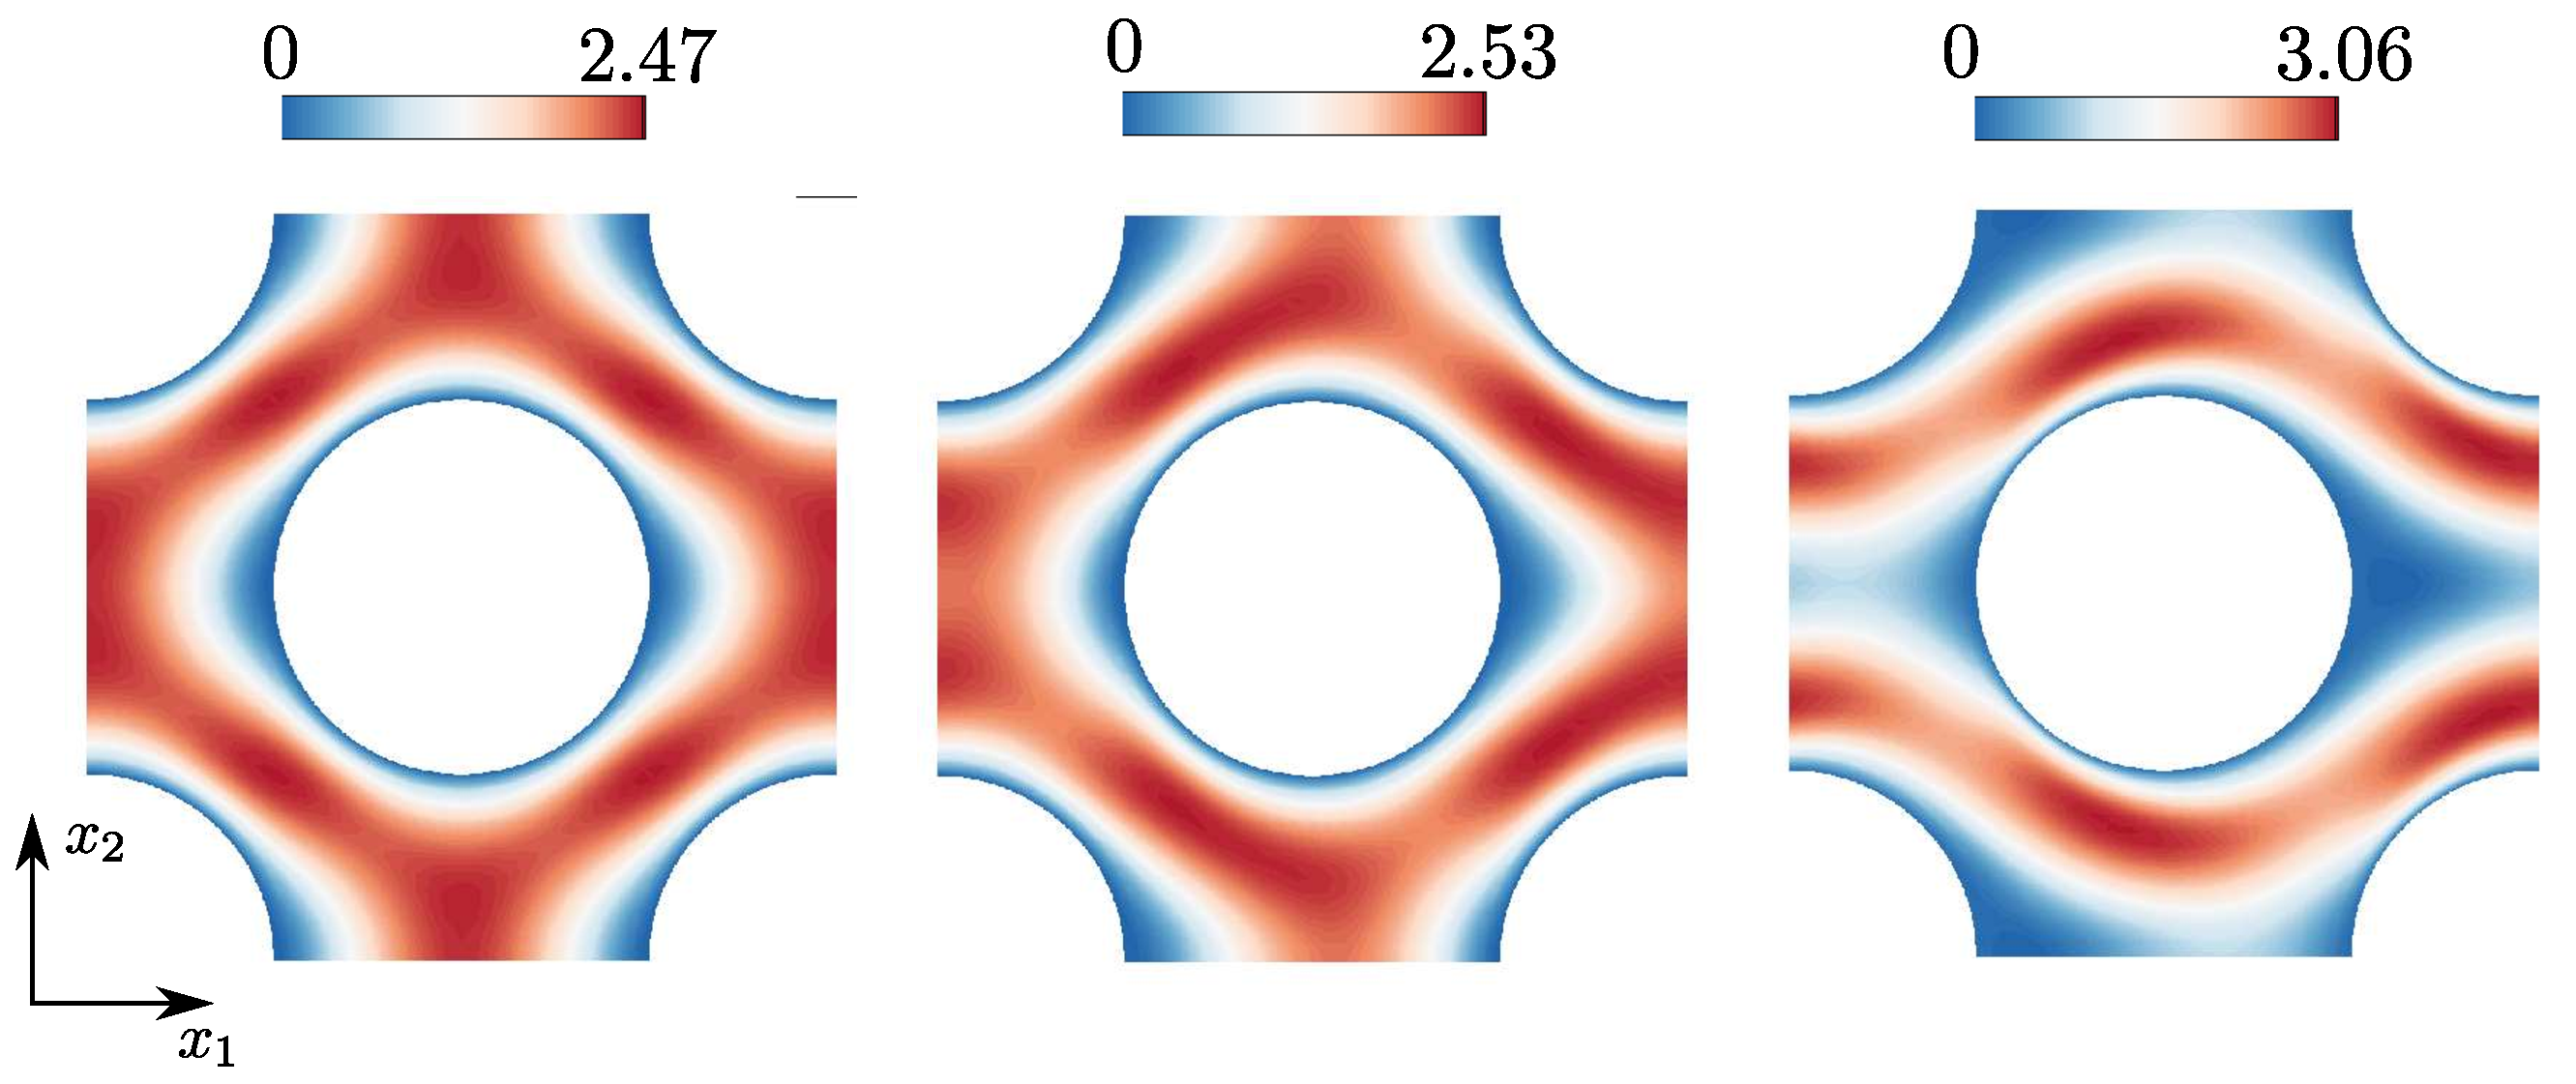
\includegraphics[width=1\textwidth]{chapter_4/figure/fig1}
	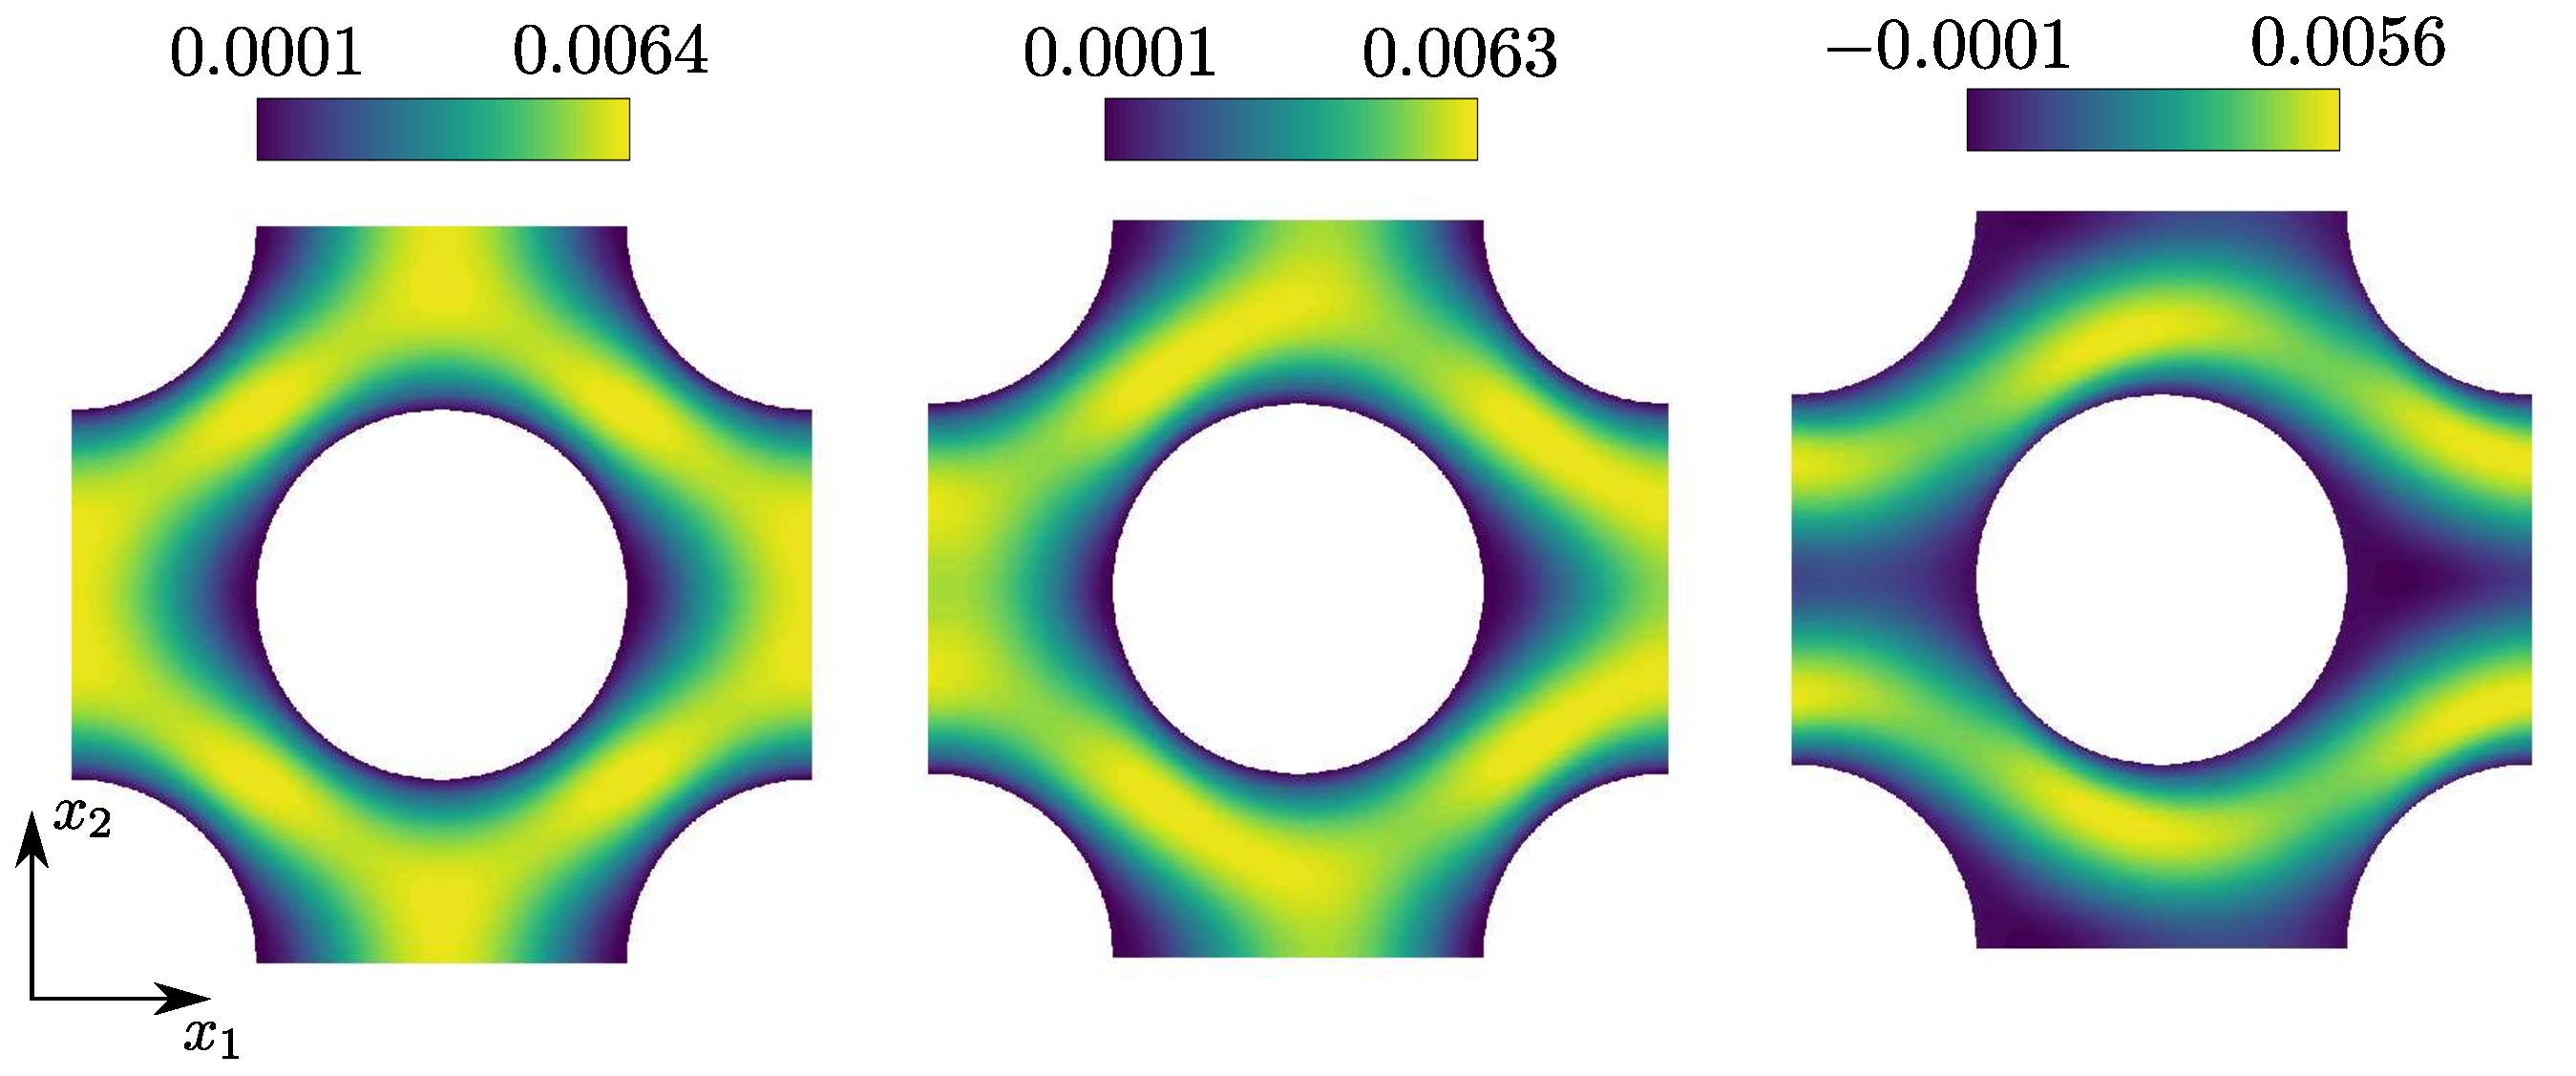
\includegraphics[width=1\textwidth]{chapter_4/figure/fig2}
	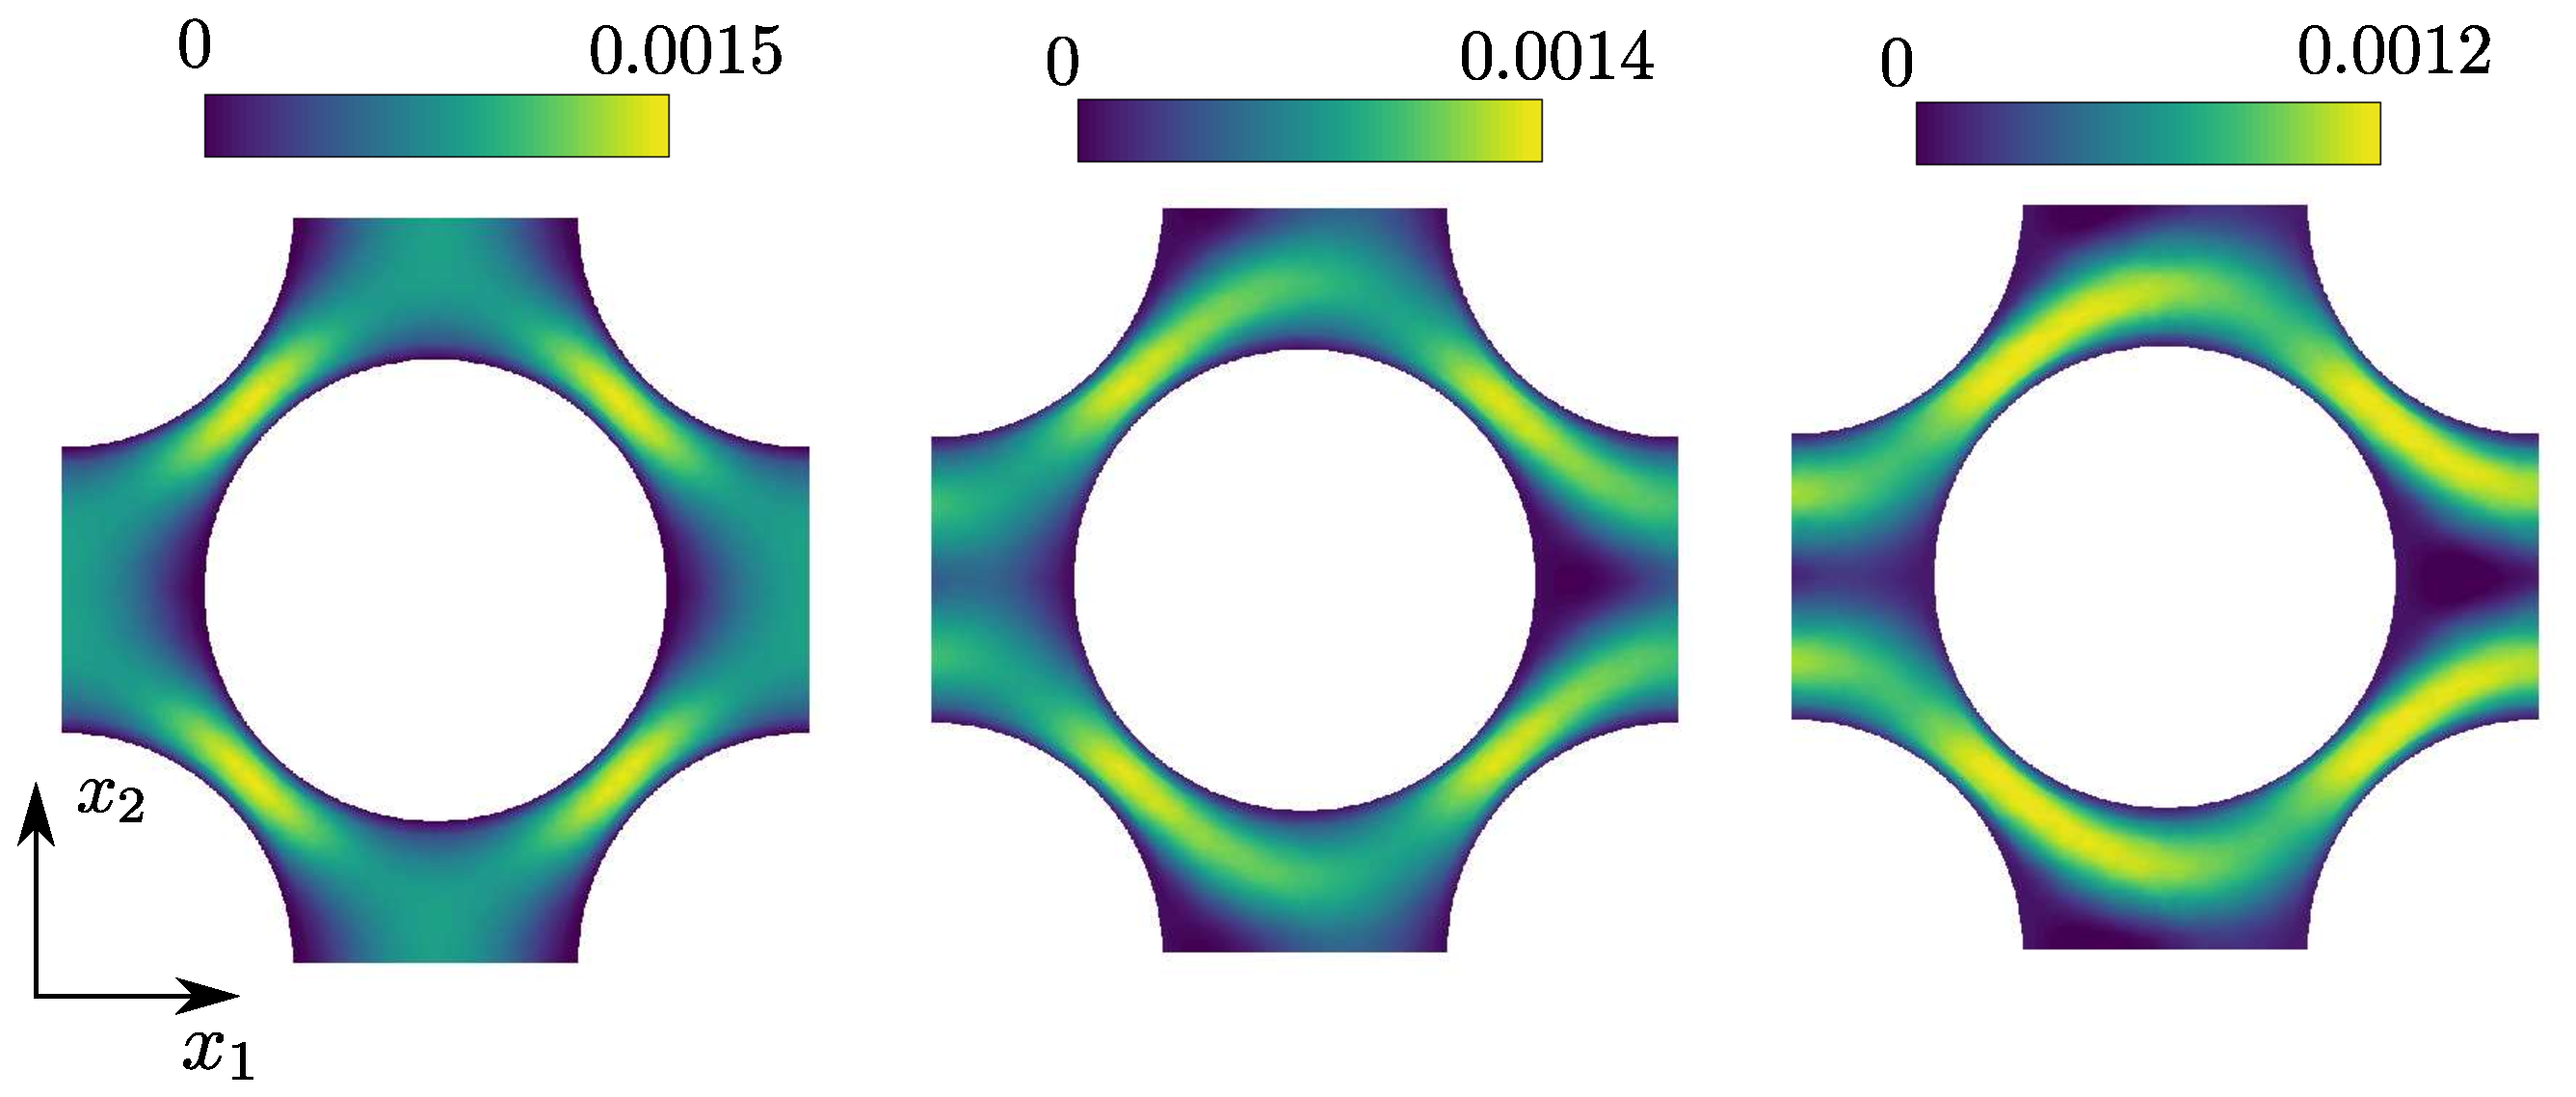
\includegraphics[width=1\textwidth]{chapter_4/figure/fig4}
	\caption{Top row: plane view of the dimensionless $x_1$ component of the local velocity field ${\vb}$ for the case $\theta=0,$ $\phi=0$, $\varepsilon=0.6$ and for three Reynolds numbers $Re_d$ = $0,10,50$, from left to right. Mid row: microscopic $M_{11}$ fields corresponding to the images in the top row. Bottom row: $M_{11}$ fields for the same Euler angles and Reynolds number as in the top two rows, and smaller porosity ($\varepsilon=0.4$).}
	\label{fig:1ch4}
\end{figure}


\newpage

Another interesting point emerges by inspection of  figure \ref{fig:3ch4} where two off-diagonal components of $\bf{M}$ are shown for two porosity 
values; the first image (left frame) represents a plane flow in the Stokes regime while the second is the plane cut of a three-dimensional 
solution in the inertial regime. Positive and negative values of the microscopic fields can be seen in both images but, once averaging is 
applied over the REV, the resulting permeability component is very close to zero (in fact, exactly equal to zero in the Stokes case).  This same features occurs for all off-diagonal terms in all cases examined, so that, within the current range of Reynolds numbers, the 
apparent permeability tensor is, to a good approximation, diagonal\footnote{In fact, there are always at least two orders of magnitude 
	differences between the diagonal and the off-diagonal components. While the latter should not, in principle, be ignored, we will focus attention 
	here only on the dominant terms of the permeability tensor.}.


\begin{figure}[H]
	\centering
	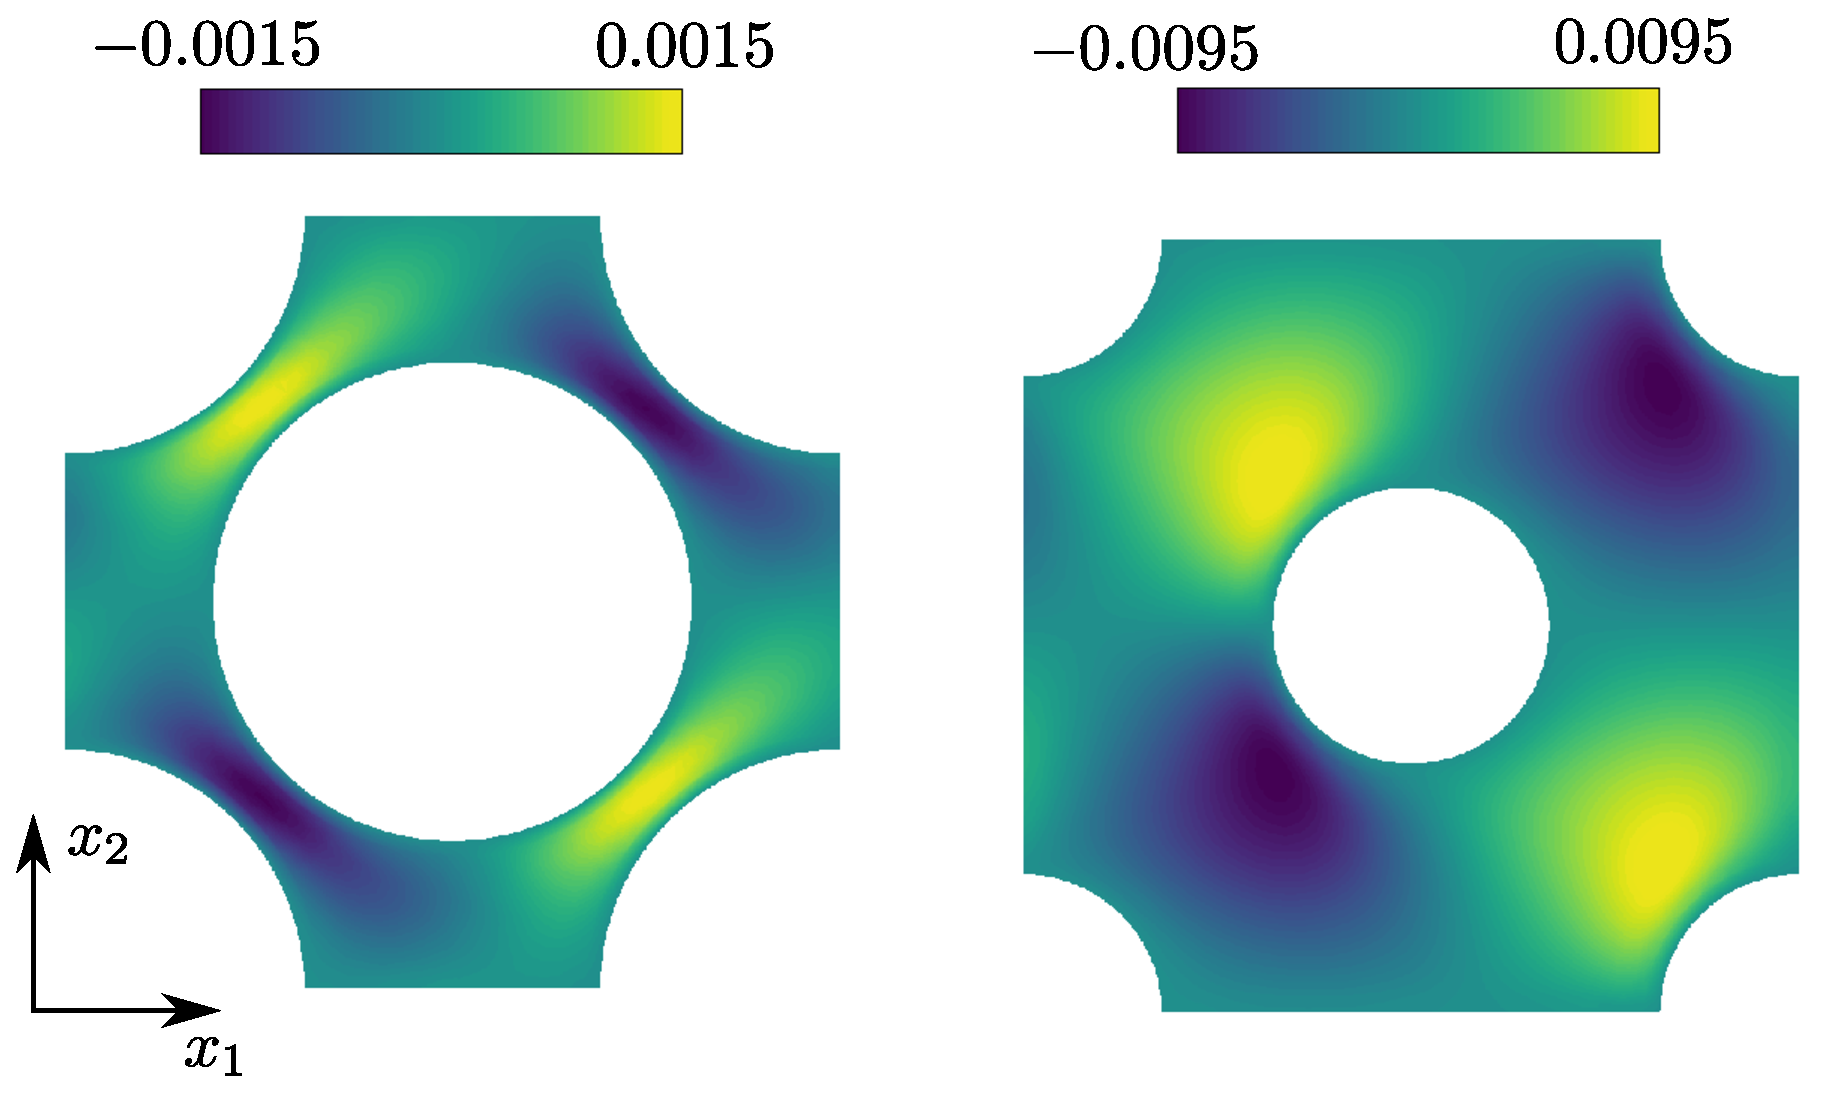
\includegraphics[width=0.8	\textwidth]{chapter_4/figure/fig3}
	\caption{right: Non-dimensional $M_{21}$ field for $\theta=0, \phi=0, Re_d=10, \varepsilon=0.8$, left: Non-dimensional $M_{12}$ field for $\theta=22.5^{\circ}, \phi=45^{\circ}, Re_d=50, \varepsilon=0.4$.}
	\label{fig:3ch4}
\end{figure}

A three-dimensional case is shown in  figure \ref{fig:5ch4}, where all the non-zero terms of the $\mathbf{M}$ tensor are plotted for a porous
structure with $\varepsilon=0.6$. The components shown are $M_{11}$, $M_{22}$,$M_{33}$, $M_{12}$ and $M_{21}$, while $M_{i3}$ and $M_{3j}$ are 
not plotted because they are identically zero to machine accuracy. Distinct features are visible in each image; in particular, in the last 
frame the $M_{33}$ microscopic component displays a low wavelength structure along the cylinder's axis. Increasing the dimensions of the REV 
along $x_3$ does not alter such a structure, i.e. the $\ell^3$ domain chosen with its periodic boundary conditions does not filter out 
significant high wave-numbers of the flow. We further note that the tensor $\mathbf{M}$ is not symmetric in this case since each off-diagonal component 
represents the solution of the closure problem in a specific direction (first index of the field) and the forcing term acts orthogonally to it
(second index of the field).  Once averaged over the REV it is found that both $H_{12}$ and $H_{21}$ are very close to zero.  


\begin{figure}[H]
	\centering
	\includegraphics[width=0.75\textwidth]{chapter_4/figure/fig5}
	\caption{Non-dimensional $\mathbf{M}$ components fields for the case $\theta=22.5^{\circ}, \phi=45^{\circ}, Re_d=50, \varepsilon=0.6$.}
	\label{fig:5ch4}
\end{figure}    






%%%%%%%%%%%%%%%%%%%%%%%%%%%%%%%%%%%%%%%%%%%%%%%%%%
\section{The apparent permeability tensor}
%%%%%%%%%%%%%%%%%%%%%%%%%%%%%%%%%%%%%%%%%%%%%%%%%%

\label{sec:5}

In this section the variations of the diagonal components of the permeability tensor $\mathbf{H}$ are discussed as function of the direction of 
the mean forcing, the Reynolds number and  the porosity. As stated previously, the Reynolds number ranges from $0$ to approximately $100$ in 
order to capture phenomena associated with inertia; the cases considered never lead to unsteady signals. 
The porosity parameter $\varepsilon$ is set to either $0.4$ (low porosity),  $0.6$ (medium) or
$0.8$ (high). The forcing direction is defined by the Euler angles and all the configurations considered in this section are summarized in 
table \ref{table:directions}; the choice has been made to explore a reasonably large range of parameters, with both two-dimensional and three-
dimensional flows characterized by symmetric and asymmetric patterns.

Let us briefly recall the methodology. First, a DNS is carried out to compute the microscopic flow. Then the  closure problem is solved for the 
tensor $\mathbf{M}$. Finally, each component of the apparent permeability  $\mathbf{H}$  is obtained by averaging (equation 
\eqref{eq:avg_intrinsic}).
The results are collected in figures \ref{fig:08_H}, \ref{fig:06_H} and \ref{fig:04_H}, showing the variation of the diagonal components 
of $\mathbf{H}$. 


\begin{table}[t]
	\centering
	\begin{tabular}{l | l l l}
		index & $\theta$ & $\phi$ & field properties \\\hline	\hline
		1 & $0^\circ$ & $0^\circ$ & 2D symmetric \\
		2 & $22.5^\circ$ & $0^\circ$ & 2D non-symmetric \\
		3 & $0^\circ$ & $45^\circ$ & 3D symmetric \\
		4 & $22.5^\circ$ & $45^\circ$ & 3D non-symmetric \\
		5 & $-$ & $90^\circ$ & 3D symmetric \\
		\hline  
	\end{tabular}
	\caption{Directions of the forcing tested and property of the solutions.}
	\label{table:directions}
\end{table}



\begin{figure}[H]
	\centering
	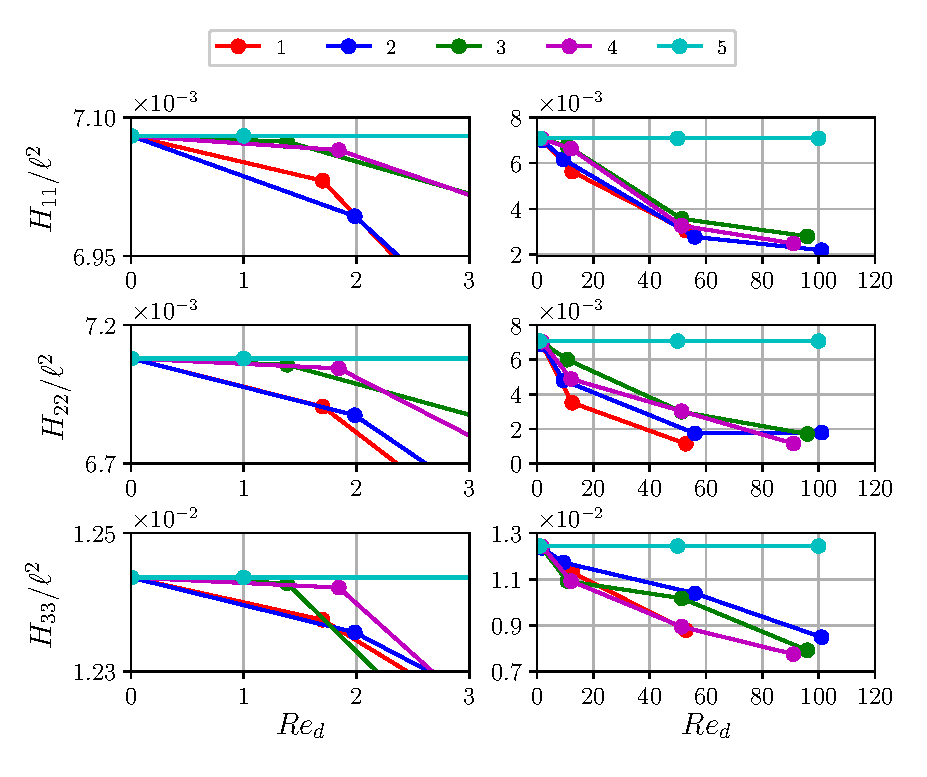
\includegraphics[width=1\textwidth]{chapter_4/figure/H_of08}
	\caption{Diagonal elements of the apparent permeability $\mathbf{H}$ as function of the Reynolds number for porosity  $\varepsilon=0.8$. The forcing  direction is represented through the couple of Euler  angles 
		$(\theta,\phi)$ (cf. table \ref{table:directions} for the case index). Left column: low-$Re_d$ regime; right column: inertial regime.}
	\label{fig:08_H}
\end{figure} 

\begin{figure}[H]
	\centering
	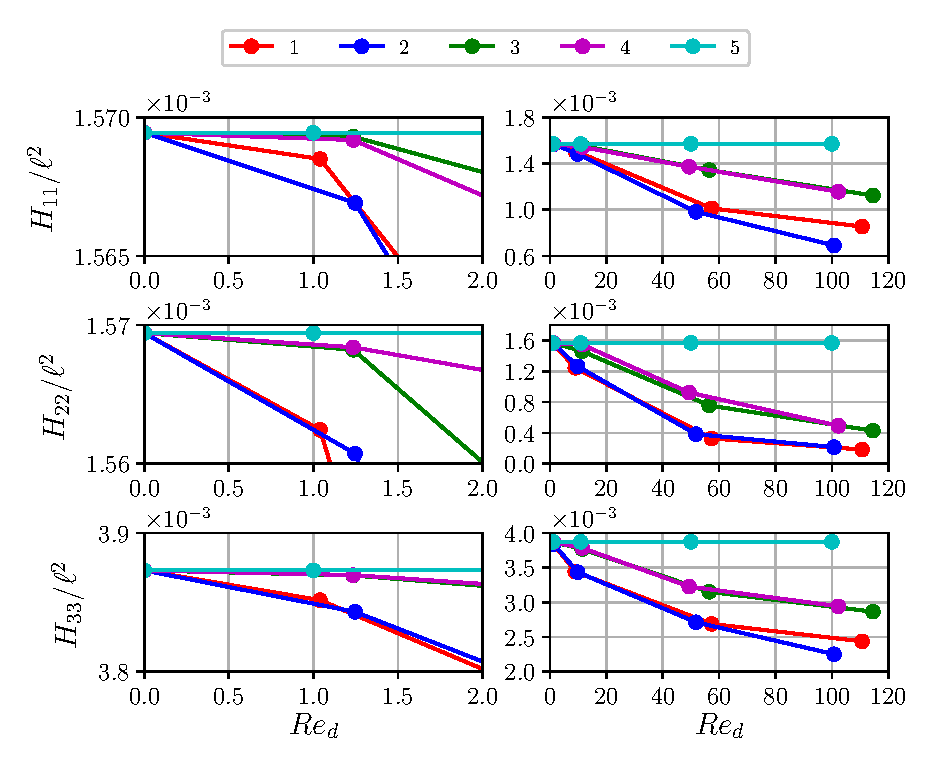
\includegraphics[width=1\textwidth]{chapter_4/figure/H_of06}
	\caption{Same as figure \ref{fig:08_H} with porosity $\varepsilon=0.6$.}
	\label{fig:06_H}
\end{figure}



\begin{figure}[H]
	\centering
	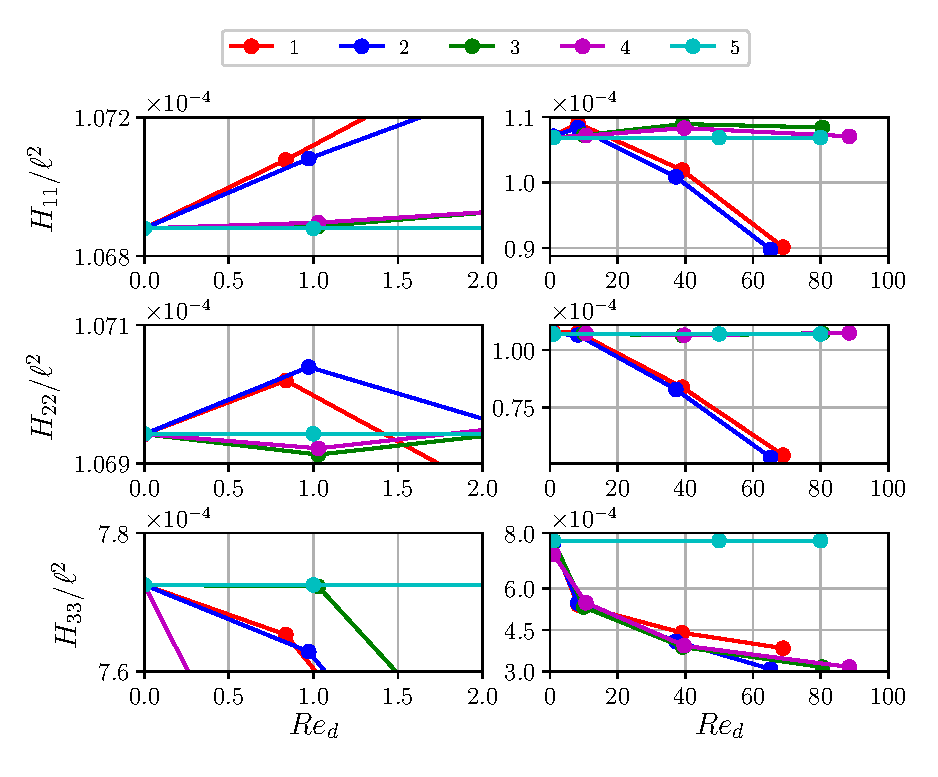
\includegraphics[width=1\textwidth]{chapter_4/figure/H_of04}
	\caption{Same as figure \ref{fig:08_H} with porosity $\varepsilon=0.4$.}
	\label{fig:04_H}
\end{figure}

%\begin{figure}[H]
%   \centering
%   \input{figure/H_of04.pdf_tex}
%   \caption{Same as figure \ref{fig:08_H} with porosity $\varepsilon=0.4$.}
%   %\label{fig:04_H}
%\end{figure}
%



In the left column of each figure we focus on the low-$Re_d$ regime ($0 < Re_d < 2$), while in the right column the effect of inertia can be 
assessed.  As expected, when $Re_d$ is small the apparent permeability is quasi-Reynolds-number-independent (and can be approximated well by 
the true permeability). As the Reynolds number increases above a few units, inertial effects grow in importance yielding typically a monotonic decrease of all 
components of $\mathbf{H}$, aside from case indexed 5 ($\phi=90^{\circ}$) for which the flow remains aligned with the cylinder's axis. In case 5 the 
microscopic flow solution is invariant with $x_3$ and does not change with $Re_d$ in the range considered, so that $\mathbf{H}$ is a  
constant tensor.

When the porosity is large all components show a similar behaviour irrespective of the forcing angle (except, clearly, case 5). Differences 
start appearing at $\varepsilon=0.6$; the two cases with $\phi=0^{\circ}$ (index 1 and 2) behave similarly, and so do the two cases indexed 3 
and 4 (with $\phi=45^{\circ}$). This seems to suggest a weaker effect of $\theta$ on the permeability components.  For even smaller porosity ($
\varepsilon=0.4$), the blockage which the inclusions cause to the flow produces the unexpected behaviour displayed in figure \ref{fig:04_H}. 
When the flow is purely two-dimensional (cases 1 and 2), variations in the Reynolds number affect $\mathbf{H}$ significantly; when a pressure 
gradient along $x_3$ is present the strong packing of the fibers constrain the fluid to flow prevalently along the fibers' axis, and the 
apparent permeability is almost $Re_d$-independent. When assessing variations in $H_{jj}$ for this case, attention should also be paid to the 
fact that the permeability is now at least one order of magnitude smaller than in the previous cases so that variations of the diagonal 
components shown in figure \ref{fig:04_H} are tiny in absolute terms.  This is related to the fact that  the  inverse of the permeability  
plays the role of a drag coefficient in the macroscopic expression of the force  (cf. equation \eqref{eq:macroscale}).  In other words, 
materials with higher porosity (larger space between solid inclusions) offer lower resistance to the motion of the fluid.


%In the simulations carried out the off-diagonal terms are consistently at least two orders of magnitude smaller than their diagonal 
%counterparts, for all parameters considered.  
Applying the intrinsic average operator to the non-diagonal component of the tensor $\mathbf{M}$ results in terms that are negligible with respect to their diagonal counterparts, and these results are true for all the parameters considered. This means that there is a very weak coupling between the principal directions of the fiber.
The directional decoupling and the diagonal property of the apparent permeability tensor has also been computationally demonstrated
on a completely different REV geometry by \citet{soulaine2014}. Conversely,
\citet{lasseux} have carried out a two-dimensional study with fibers of square cross-section, finding that the off-diagonal terms are 
non-negligible and only about
one order of magnitude smaller than the diagonal components. This result is a consequence of the non-rotationally-invariant  geometry  
considered.  The present work and the two articles just cited suggest that the  diagonal property of the tensor $\mathbf{H}$   is closely
related to the geometry of the porous material, more  than to the flow regime.  



%%%%%%%%%%%%%%%%%%%%%%%%%%%%%%%%%%%%%%%%%%%%%%%%%%%%%%%%%%%
\section{A metamodel for $\bf H$}
%%%%%%%%%%%%%%%%%%%%%%%%%%%%%%%%%%%%%%%%%%%%%%%%%%%%%%%%%%%

The previous sections has shown how the apparent permeability depends on  the two Euler angles, the Reynolds number and the porosity. The space 
of parameters is formidable and the results found so far are not sufficient to treat, for example, cases characterized by multiple inclusions'
sizes and orientations in different regions of the domain, or cases involving a poroelastic medium, with temporally and spatially varying 
porosity, flow direction and local Reynolds number. The complete solution of the closure problem for a single set of parameters takes 
approximately 4 CPU hours on our two-processor Intel(r) IVYBRIDGE 2.8Ghz, each with 10 cores and 64 GB of RAM, so that a complete parametric 
study is, to say the least, unpractical. In view of this, the construction of a metamodel capable to provide a full characterisation of the 
permeability as a function of all parameters is a worthy endeavor. We have tested several surrogate models, before eventually settling on the kriging 
approach \cite{Kleijnen20171} described in the following.



%Usually the homogenization approaches are used to investigate complex problems in which   length scales  of the physical phenomena are much %larger than the REV one (\citet{ugis})  (\citet{prosperetti}). The aim
%is to avoid to resolve the  length scales smaller the unity (with respect to the REV length) and in consequence to drastically reduce  the %number of mesh cells and the computational load.
%Here the physics at the REV scale is modelled with the VANS method and in particular by identifying the local apparent permeability $%\mathbf{H}$ tensor.

%In addition, it has been shown that the non constant tensor $\mathbf{H}$ required to be evaluated locally and at each time step  in a full %temporal simulation over a large domain with large REV numbers. 
%Especially, at at least the local Reynolds number and the flow direction change from cell to cell, where each cell could be composed of one or %several REV.

%Solving the $\mathbf{H}$ closure problem for a given set of parameters takes approximately 4 hours with our resources [two processor Intel(r) %IVYBRIDGE 2,8Ghz each with 10 cores and 64 GB of RAM], so reiterate the procedure inside each time step for each cell is at least unpractical. 
%
%To circumvent such a problem  the design of a reduce order model, or the use of a metal-model can be a convenient approach.  
%In this work, several metamodel have been investigated and only one is presented in the following.


%%%%%%%%%%%%%%%%%%%%%%%%%%%%%%%%%%%%%%%%%%%%%%%%%%%%%%%%%%%
\subsection{DACE sampling}
%%%%%%%%%%%%%%%%%%%%%%%%%%%%%%%%%%%%%%%%%%%%%%%%%%%%%%%%%%%


The first step to build a metamodel is the collection of relevant samples.
The quality of the final metamodel strongly depends on the samples collected and their number and distribution is of primary importance.
The apparent permeability tensor, $\mathbf{H}$, depends on  four independent variables; the samples  have been generated starting from 
the set of parameters given in table \ref{table:DACE}.

\begin{table}[t]
	\centering
	\begin{tabular}{l | l l l l l}
		parameter & values \hs{0.5} & \hs{1.5}       &  \hs{1.5}     &\hs{1.5}   &\hs{1.5}  \\ \hline \hline
		$\theta$  & $0^\circ$     & $22.5^\circ$ & $45^\circ$  &  & \\
		$\phi$    & $0^\circ$     & $22.5^\circ$ & $45^\circ$  & $67.5^{\circ}$ & $90^{\circ}$ \\
		$Re_d$ & $0$ & $10$ & $50$ & $100$ \\
		$\varepsilon$ & $0.4$ & $0.6$ & $0.8$ \\
		\hline  
	\end{tabular}
	\caption{Sampling parameters.}
	\label{table:DACE}
	
\end{table}

One of the best options to generate the relevant database would be to use a full factorial design approach
in which all the combinations of the four variables from table \ref{table:DACE} are computed. Because of the large number of computations required, this approach has not been retained. We have resorted to the methodology known as DACE (Design and Analysis of
Computer Experiments), a technique to fill in the best possible way the space of the parameters of the problem.
%
%Actually, to be more efficient, we have to use the methodologies developed for the design and analysis of computer experiment refers as DACE. %DACE models 
%are canonical methods that fills in the best way the space parameters of the problem, knowing  the number of variables and their discrete %values. 
The Dakota library \cite{dakota} has been selected for the purpose and 
the Monte-Carlo incremental random sampling algorithm \cite{giunta} has been chosen, in order to make efficient use of the cases
already computed. This incremental approach selects in a quasi-random way the new samples to generate, starting from the existing ones. In the end, the set of samples comprises 118 cases.


% to keep the advantage of the previous simulations and to decrease the number of new cases to carry out.
%Stating from the previous samples already computed, 30 new sampling have been generated by the algorithm that fill the parameters space in a %quasi-random way. 
%Each new sampling parameters depends on the previous set.
%
%For each new parameters combination we repeating the computational procedure explained before to compute the permeability tensor  $\mathbf{H}$.



\begin{figure}[H]
	\centering
	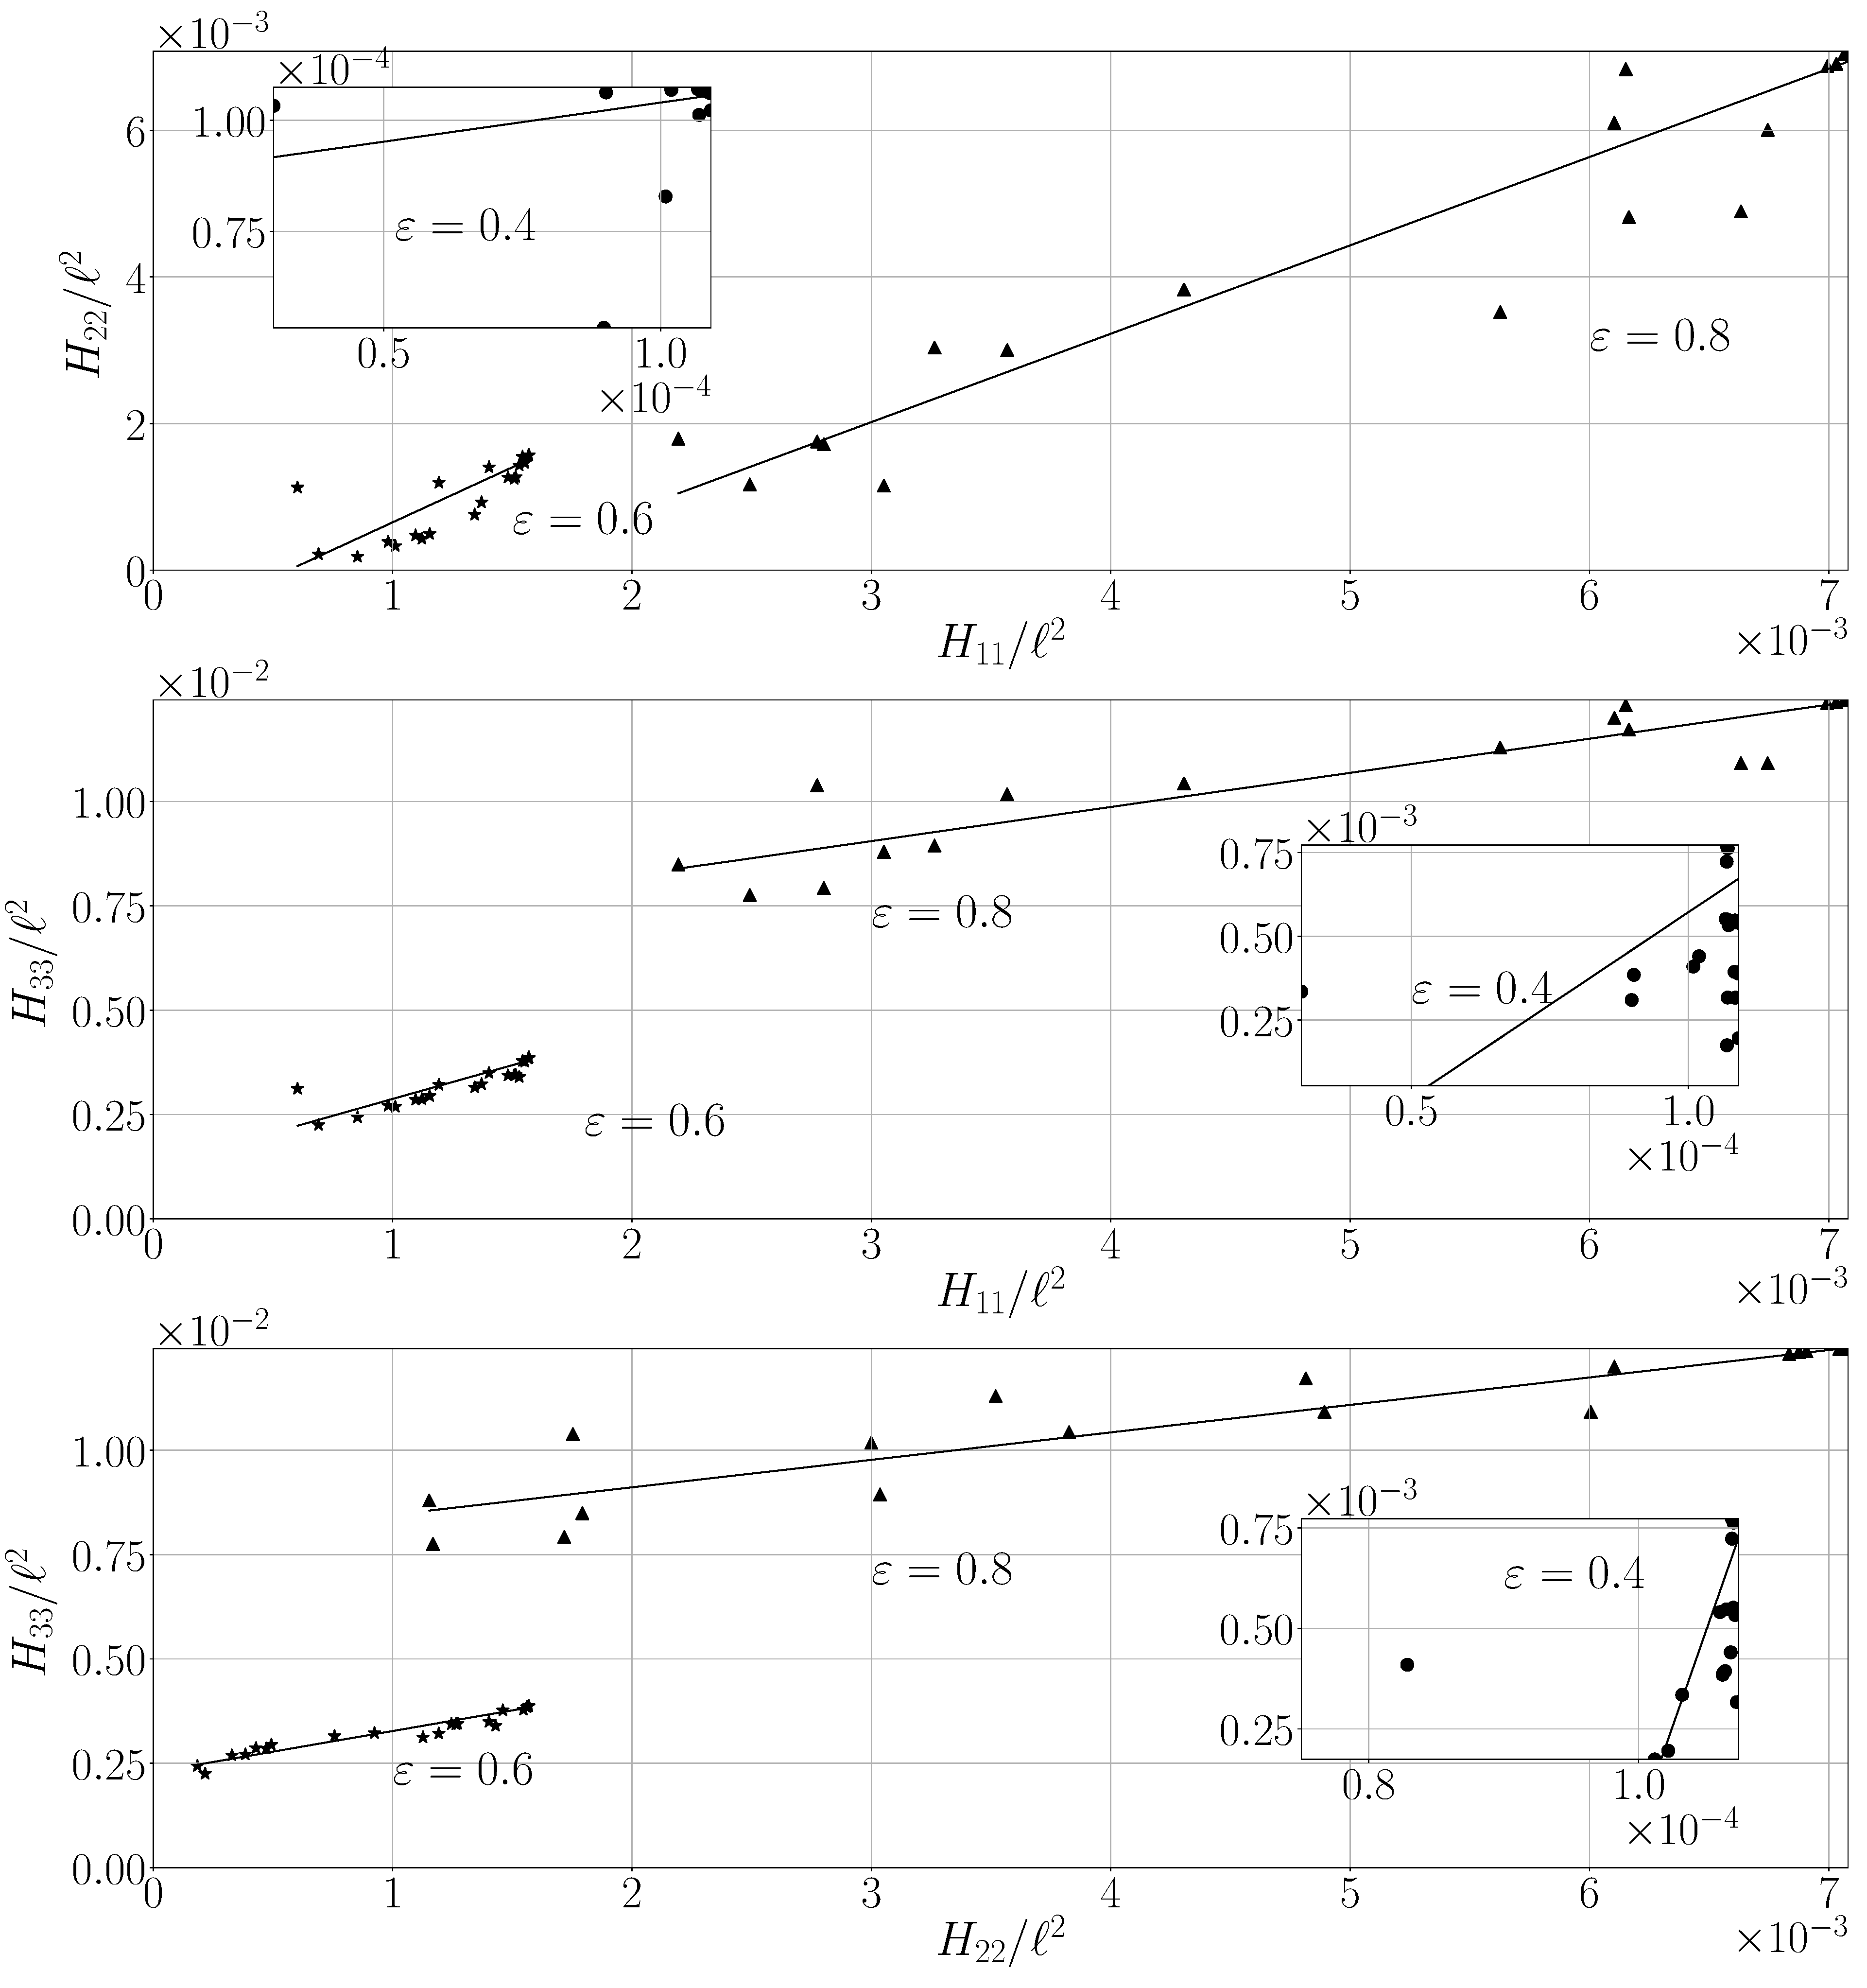
\includegraphics[width=1\linewidth]{chapter_4/figure/scatter_matrix}
	\caption{Scatter matrix plot for the collected numerical data of the apparent permeability tensor.}
	\label{fig:scatter_matrix}
\end{figure}



In the scatter plot of figure \ref{fig:scatter_matrix} the three diagonal components of the permeability tensor are shown 
as function of one another. The three porosities are separately considered in each of the above plot, and the permeability points are 
represented with their linear regression on top. This kind of plot is common in statistical analysis to determine if correlations in the data 
are present.  The permeability components show some correlation with the data points which lie reasonably well on a straight line. This
result has a physical implication.
Remembering the diagonal dominance of the permeability tensor, we have in the low
$Re_d$ limit: 

\begin{equation}
\left( \meani{u_{\beta}},\meani{v_{\beta}} , \meani{w_{\beta}}\right) \sim \left(H_{11} \dfrac{{\partial p}}{\partial x_1}, H_{22} \dfrac{{\partial p}}{\partial x_2} ,  H_{33} \dfrac{{\partial p}}{\partial x_3}\right).
\label{eq:linear_k}
\end{equation}
$$ \, $$
\noindent It is then possible to compute the angle between the forcing term, $\nabla p$, and the average velocity vector, represented 
in  figure \ref{fig:diag_rel} for the two-dimensional case, $\phi = 0$. This is achieved by taking the ratio between the
first two components of Darcy's equation, calling $\gamma$ the flow deviation with respect to the mean forcing. We thus have:

\begin{equation}
\tan \, (\theta + \gamma) = \dfrac{H_{22}}{H_{11}} \tan \, \theta.
\label{eq:angles}
\end{equation}

\noindent If the ratio between the two permeability components is equal to one, the angle $\gamma$ vanishes.
The correlation between $H_{11}$ and $H_{22}$ controls the deviation of the flow in the $(x_1, x_2)$ plane, and the argument
can easily be extended to $H_{11}/H_{33}$ and $H_{22}/H_{33}$  for deviation angles in three-dimensions.

\begin{figure}[H]
	\centering
	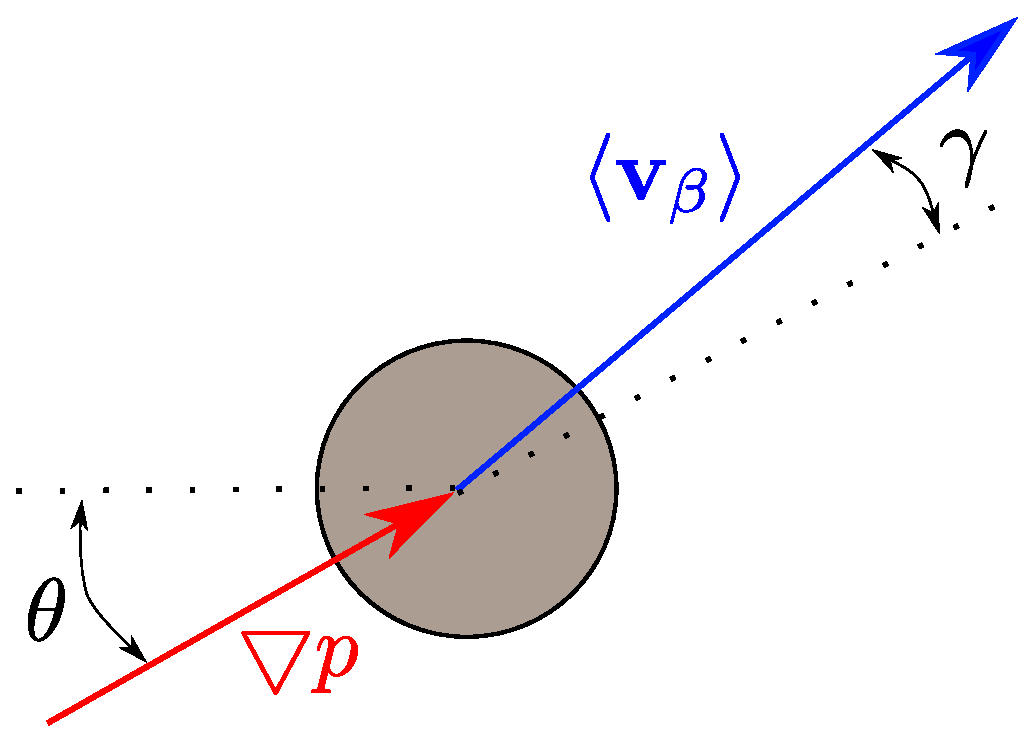
\includegraphics[width=0.45\linewidth]{chapter_4/figure/k11_k22_relation}
	\caption{Explanatory sketch for the relation between mean pressure gradient and mean velocity field.}
	\label{fig:diag_rel}
\end{figure}


\begin{table}[t]
	\centering
	\begin{tabular}{ l | l   l   l   }
		$\varepsilon$ & $H_{11}/H_{22}$ \hs{1} & $H_{11}/H_{33}$ \hs{1} & $H_{22}/H_{33}$ \hs{1} \\ \hline \hline
		0.4 & 1.57 & 11.06 & 96.03 \\ 
		0.6 & 1.50 & 1.62 & 0.99 \\
		0.8 & 1.20  & 0.82 & 0.66 \\ \hline
	\end{tabular}
	\caption{Permeability components ratio for three values of the porosity. The permeability ratios here are given by the angular coefficients of the linear correlations displayed in figure \ref{fig:scatter_matrix}.}
	\label{table:ratio}
\end{table}

Using a linear correlation such as that shown in table \ref{table:ratio} and  figure \ref{fig:scatter_matrix}, it is 
observed that in the low porosity case $(\varepsilon=0.4)$ the ratio can become very large indicating a strong deviation of the flow from the forcing direction, because of the strong constraint provided by the inclusions. As the porosity increases, the ratio does not differ much from unity, which means that the deviation remains limited. It is simple to see that
the deviation angle, for example in the $(x_1, x_2)$ plane, satisfies the approximate relation
$$
\tan \, \gamma = \dfrac{\left(1 - \dfrac{H_{11}}{H_{22}}\right) \tan \, \theta}{\dfrac{H_{11}}{H_{22}} + \tan^2 \, \theta},
$$
so that for $\dfrac{H_{11}}{H_{22}}$ equal to, say, 1.5, the largest deviation remains always below $12^{\circ}$ for any $\theta$.
It should however be kept in mind that trends based on these ratios are valid only as long as Darcy's law and linear correlations
are acceptable. Cases exists for which such trends are violated; for example, a flow with $\theta = 45^{\circ}$ and $\phi = 0^{\circ}$ has
deviation angle $\gamma$ equal to zero, for whatever porosity. In this case $H_{11}/H_{22}$ is equal to one and such a point is an 
outlier in the regression plots of figure \ref{fig:scatter_matrix}.


%%%%%%%%%%%%%%%%%%%%%%%%%%%%%%%%%%%%%%%%%%%%
\subsection{Kriging interpolation method}
%%%%%%%%%%%%%%%%%%%%%%%%%%%%%%%%%%%%%%%%%%%%

The kriging approach is a linear interpolation/extrapolation method that aims to build a predictor field
based on a set of observations  $(\mathbf{x_i}, y(\mathbf{x_i}))$,  for $i=1,...,n$. 

The predictor $\hat{f}(\mathbf{x})$ is a sum of a trend function $t(\mathbf{x})$ and a Gaussian process error model $e(\mathbf{x})$:
\begin{equation}
\hat{f}(\mathbf{x}) = t(\mathbf{x}) + e(\mathbf{x}).
\label{eq:Kriging}
\end{equation}
The aim of the error model is to make adjustments on the trend function so that,
for any point of the sampling
%, equation \eqref{eq:Kriging} is strictly verified,
the predictor is  exactly equal to the sample, 
i.e. $\hat{f}(\mathbf{x_i}) = y(\mathbf{x_i})$. This property represents one of the main qualities of this approach. In addition, 
when  the model parameters are  conveniently  set,  the trend function and the covariance model can take into account both smooth and steep variations in the data set.


The trend function defined  here is  based on a second order least-square regression, with the coefficients found from 
the solution of the associated linear system.
The Gaussian process error model has zero-mean and its covariance between two generic data-points, $x_i$ and $x_j$, is written as 
$$
\textrm{Cov}(y(\mathbf{x_i}), y(\mathbf{x_j})) = \sigma^2 r(\mathbf{x_i}, \mathbf{x_j}).
$$
The coefficient $\sigma$ is an amplitude parameter and $r(x^i, x^j)$ is a correlation function, based on the Mat\'ern covariance model that reads:
\begin{equation}
r(\mathbf{x_i}, \mathbf{x_j}) =  \dfrac{2^{1- \nu}}{\Gamma(\nu)} \  \left( \dfrac{\sqrt{2} \nu |\mathbf{x_i} - \mathbf{x_j}|}{|\bs{\lambda}|} \right)^{\nu} \ K_{\nu}\left( \dfrac{\sqrt{2} \nu |\mathbf{x_i} - \mathbf{x_j}|}{|\bs{\lambda}|} \right),
\label{eq:matern}
\end{equation}
where $K_{\nu}(.)$ is a modified Bessel function and $\Gamma(.)$ is the gamma function.
The parameters that can be used to tune the metamodel are the amplitude parameter $\sigma$, the exponent $\nu$ and the scale vector $\bs{\lambda}$.
The kriging metamodel outputs can show different behaviours for different selections of the above three parameters and their setting is thus crucial. 
The amplitude parameter $\sigma$ is chosen to be equal to $1$; larger value lead to steeper gradients and undesirable local extrema around the data points.
The vector $\bs{\lambda}=(\lambda_{\theta}, \lambda_{\phi}, \lambda_{Re_d}, \lambda_{\varepsilon} )$ is a scaling parameter for the distance $ |\mathbf{x_i} - \mathbf{x_j}|$.
In this study, through systematic variations of the parameters it is found that  the choice $\bs{\lambda}=(1.2, 1, 1, 1)$ yields acceptable results; in particular, the weight along $\theta$ 
is mildly larger than in the other directions in order to obtain smoother metamodel surfaces in this direction.
The exponent $\nu$ controls the  covariance function and more especially its gradients. 
When  $\nu = 1/2$ the covariance can be approximated by a negative exponential, $\exp(-\alpha x)$  and  when $\nu$ goes to infinity it behaves as $\exp(-\alpha x^2)$.
In the present study, the best (i.e. smoother) results are obtained for $\nu$ equal to $1.9$.
The above parameters have been chosen in order to avoid unphysical or unrealistic  behaviour of the apparent permeability such as, for instance,  negative values or 
steep, spurious local maxima/minima.
The method above is implemented in OpenTURNS and full details are provided by \citet{openturns}. 


A procedure called \textit{k}-fold, belonging to the class of cross-validation methods, has been used in order to prove the robustness of the metamodel.
The \textit{k}-fold method starts with the full database $S_n = (\mathbf{x_i}, \mathbf{y}(\mathbf{x_i}))$,  for $i=1,...,n$, split into two complementary set of size $n_1$ and $n_2$, such that $S_n = S_{n_1} \cup S_{n_2}$.
Then, a new metamodel is built using only the points present in the set $S_{n_1}$. 
For the sake of clarity, the metamodel built with only the subset $S_{n_1}$ will be called from now on $\hat{f}^{n_1}$, and the metamodel build with all the database will be indicated as $\hat{f}^{n}$.
The idea now is to use the points in the set $S_{n_2}$ as test, since they are essentially "new" for the metamodel $\hat{f}^{n_1}$.
The division of the subset is performed picking points in a random way, and is repeated $k$ times in order to rule out any possible "lucky" combination.

Thus, the metric used for the error computation is the following:
$$
\xi_{cv} = \dfrac{1}{k \; n_2}\sum_{i = 1}^{k} \sum_{j = 1}^{n_2} (\hat{f_{i}}(x_j)^{n} -\hat{f_{i}}(x_j)^{n_2} )^2 ,
$$
quantifying the quadratic error between the original metamodel and the one built each time with a different set that belongs to different folds.
The metric is also averaged over all the test points $n_2$ present in all the \textit{k} folds. 
The relative mean error can be computed as:
$$
E_{cv\%} = 100 \dfrac{\sqrt{\xi_{cv}}}{mean(|\hat{f_{i}}^{n}|)} .
$$
In our case the number of points used to test the model $n_2$ is equal to $\sqrt{N} \approx 12$ as recommended for kriging metamodels \cite{wang2007review}.
The number of folds has been varied from $5$ to $25$ and in all the cases tested the $E_{cv\%}$ has been found to decrease below $6\%$ when we use at least 16 folds (which means leaving out 7 to 8 points from the metamodel construction), which is more than acceptable to prove that our kriging method is a robust approximation.

\begin{figure}[h]
	\centering
	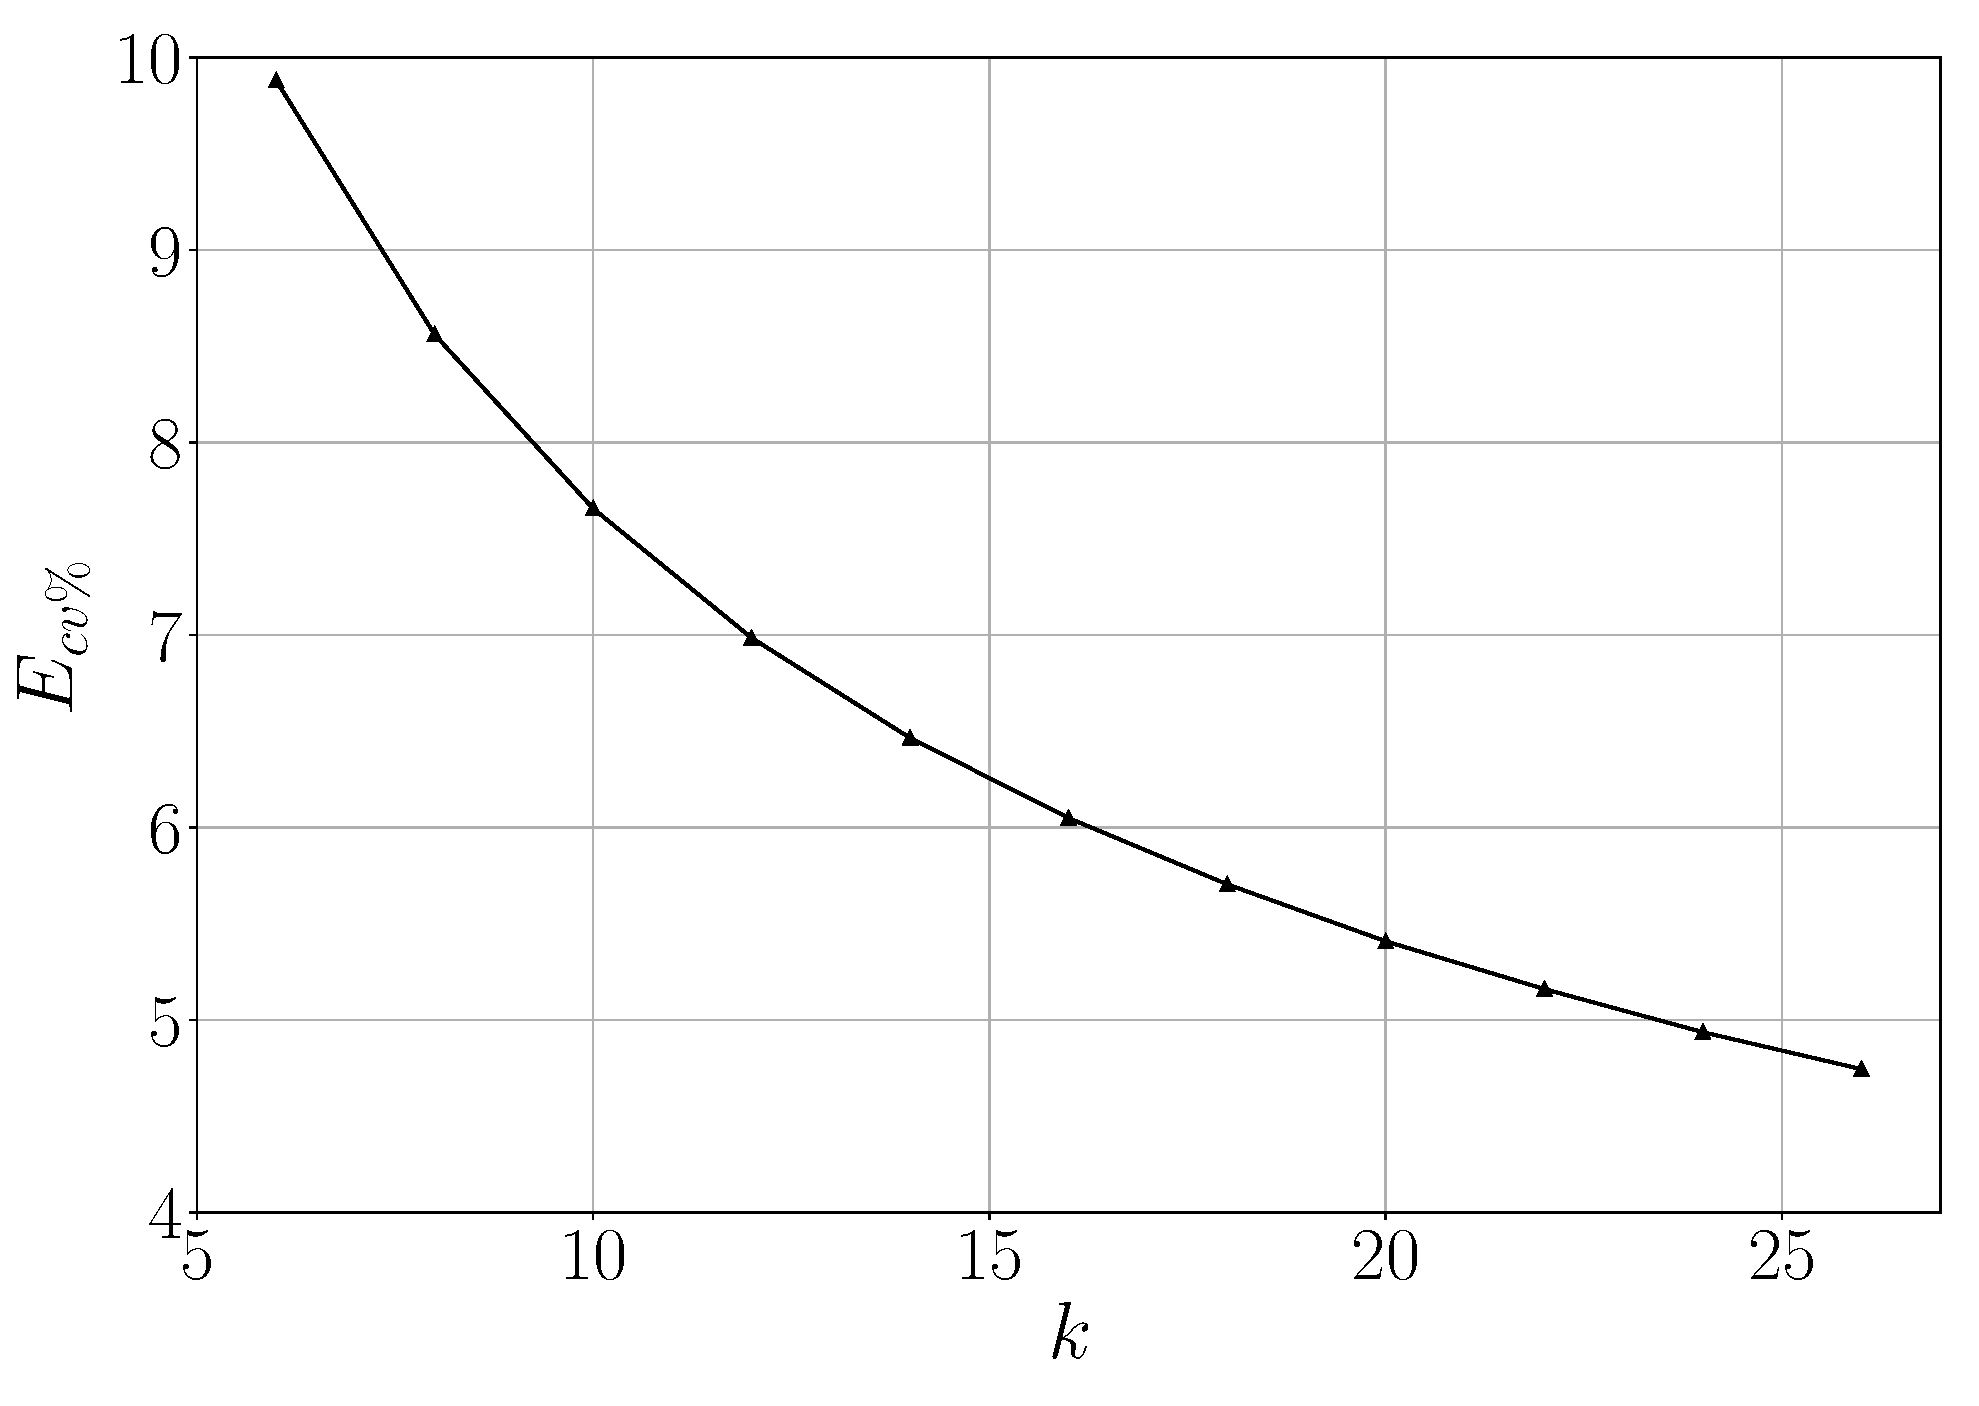
\includegraphics[width=0.7\linewidth]{chapter_4/figure/kfold_err}
	\caption{Relative mean error computed using the \textit{k}-fold approach presented against the number of folds $k$ used to divide the
		dataset}
	\label{fig:kfold_err}
\end{figure}


The metamodel provides a scalar function (for each term of the $\mathbf{H}$ tensor) defined in a four-dimensional space.
In each of the following figures  two parameters are fixed and the response surface is displayed as function of the remaining two, focussing on the  $H_{11}$ component. 
The other diagonal components of the apparent permeability tensor behave in a similar fashion and will not be shown for brevity. All the results of the metamodel are,
however, available from the authors upon request.


\begin{figure}[t]
	\centering
	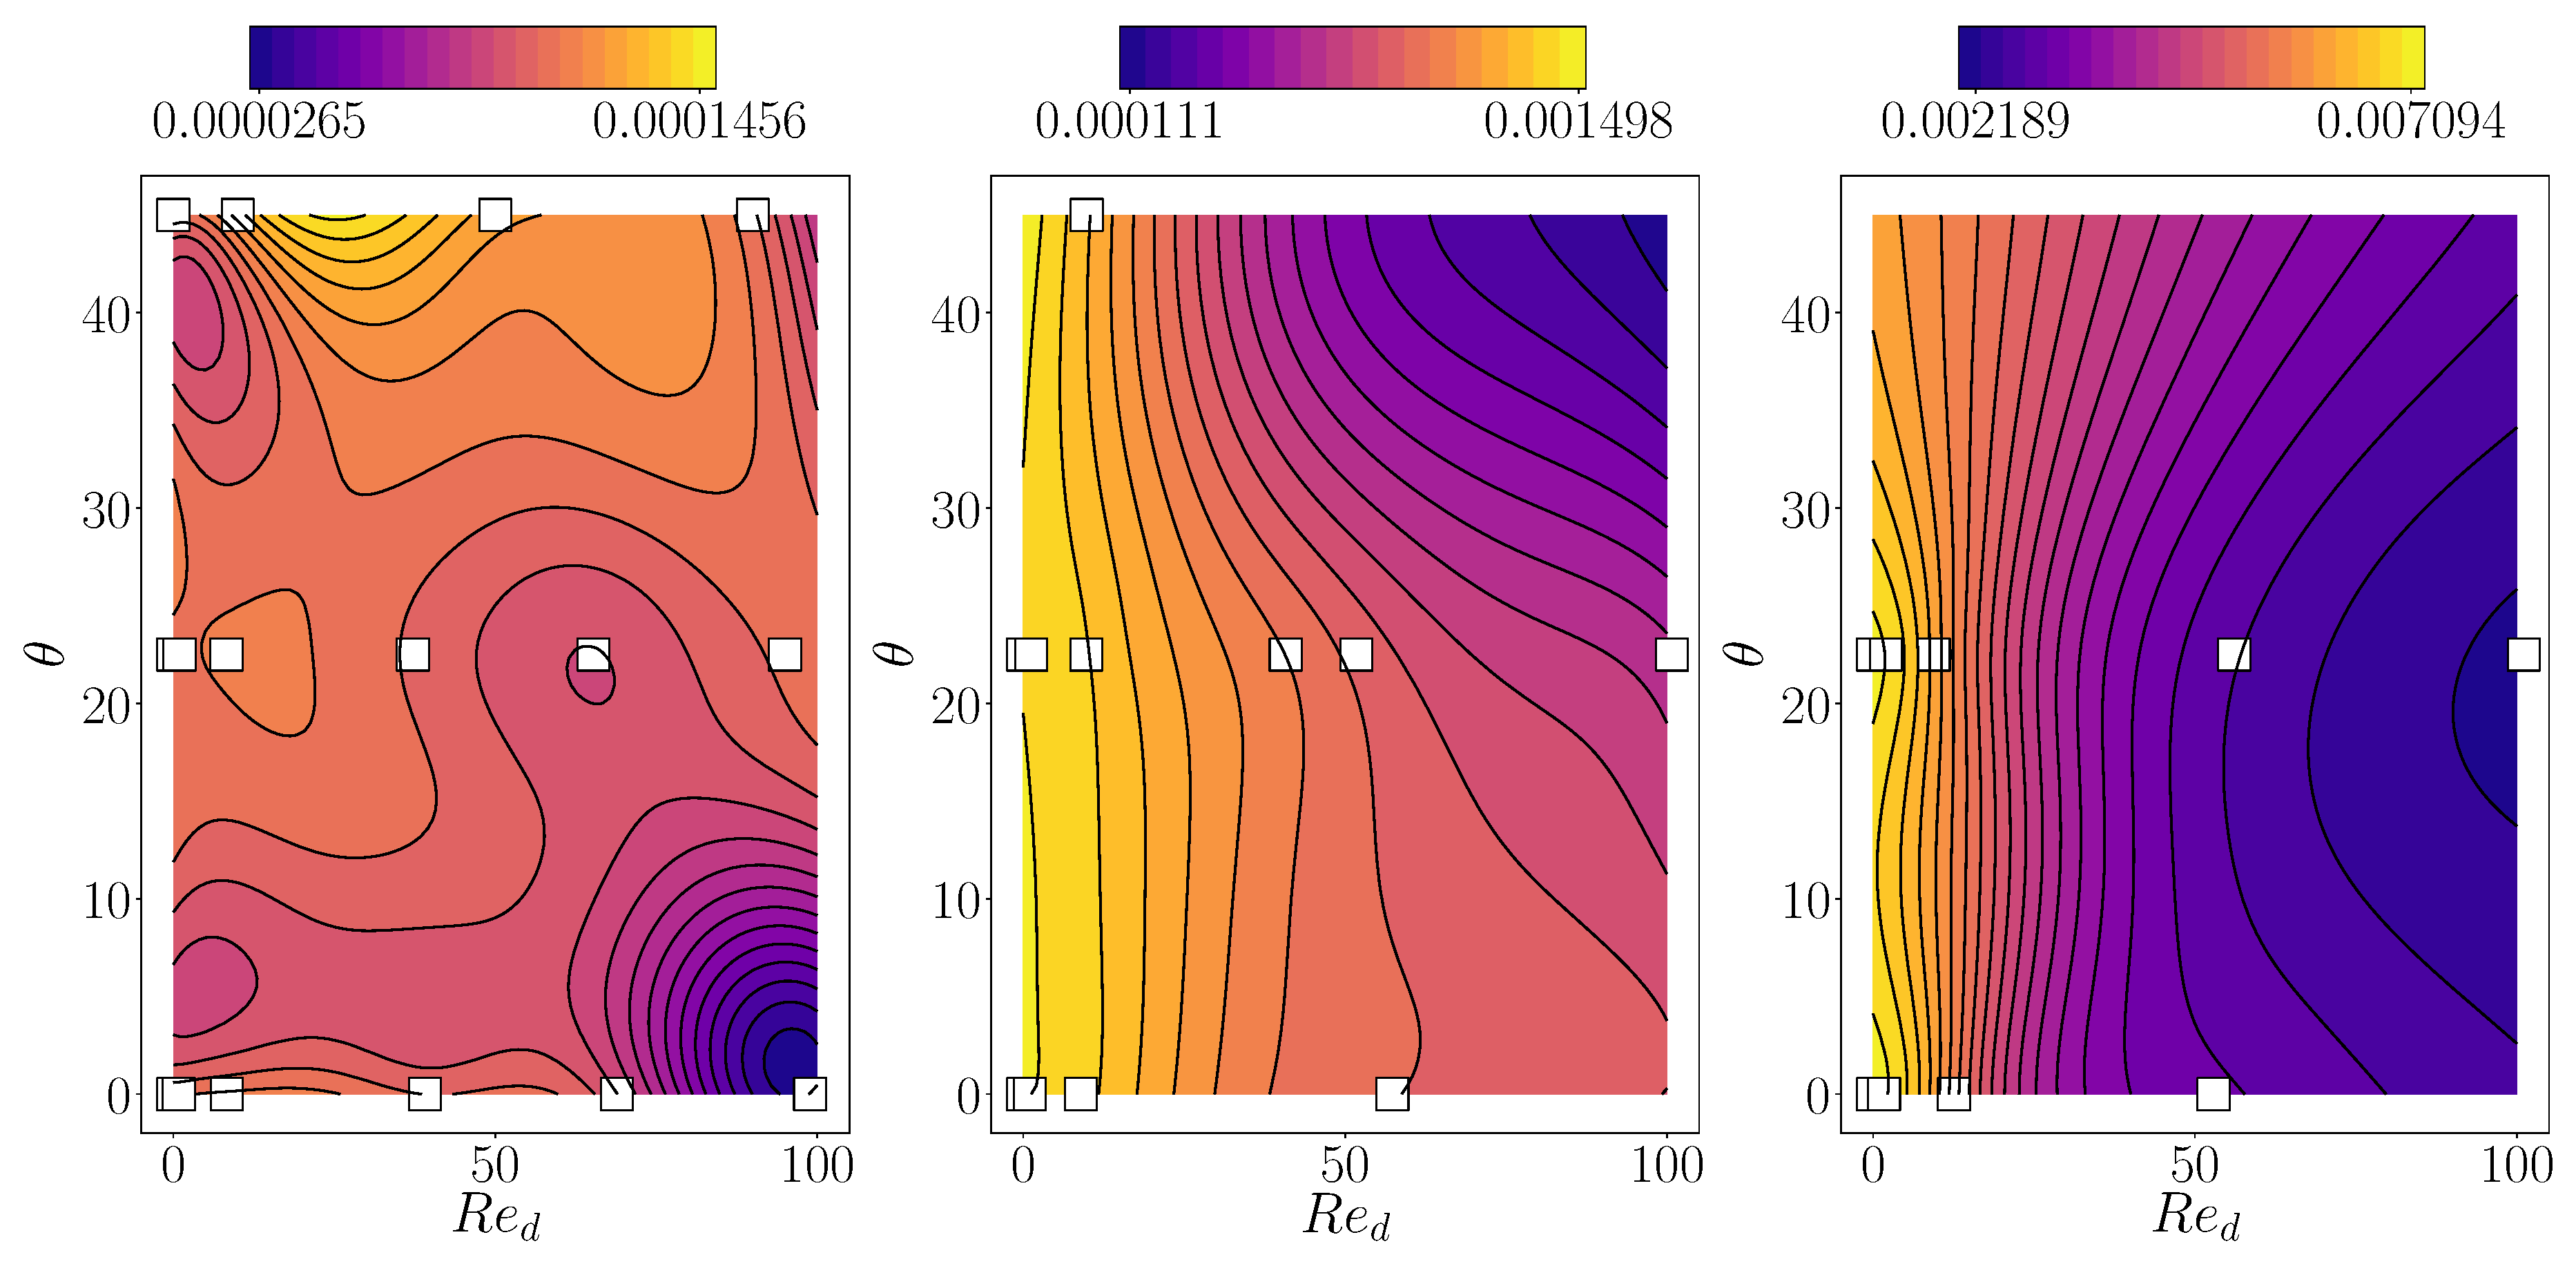
\includegraphics[width=1\linewidth]{chapter_4/figure/krig_mater_th_re}
	\caption{Response surfaces of $H_{11}$ with $\phi=0^{\circ}$ for porosity $\varepsilon=0.4, 0.6, 0.8$, from left to right.}
	\label{fig:th_re}
\end{figure}


In figure \ref{fig:th_re} the angle $\phi$ is fixed to zero, and the isolines display $H_{11}$ as function of the angle $\theta$ and of the 
Reynolds number, $Re_d$, for three  values of porosity.  The white square symbols indicate the  samples used to build the metamodel. The maximum value of 
each surface is always found for $Re_d$ equal to zero and  $H_{11}$  typically decreases with $Re_d$, when the porosity is sufficiently large.
As seen previously, for a porosity approximately greater or equal to 0.6 the variation of the  apparent permeability with the angle $\theta$ 
is weak in this two-dimensional configuration.
For the  lowest porosity studied (left frame)  the permeability has very small values and the isolines display an irregular behaviour; this is a feature
common to all plots relative to the smaller value of $\varepsilon$, signaling that it is probably necessary, in this specific case, to insert additional sample 
points in building the response surfaces. 
%Steep gradients with $Re_d$ are displayed  in the case of horizontal flow ($\theta = 0^{\circ}$).
%The observations made upon inspection of the figure are essentially the same presented in section \ref{sec:5}, and this is comforting, since it leads to
%believe in the  capacity of the metamodel to describe the trend of $H_{11} = f(\theta, Re_d)$.



\begin{figure}[t]
	\centering
	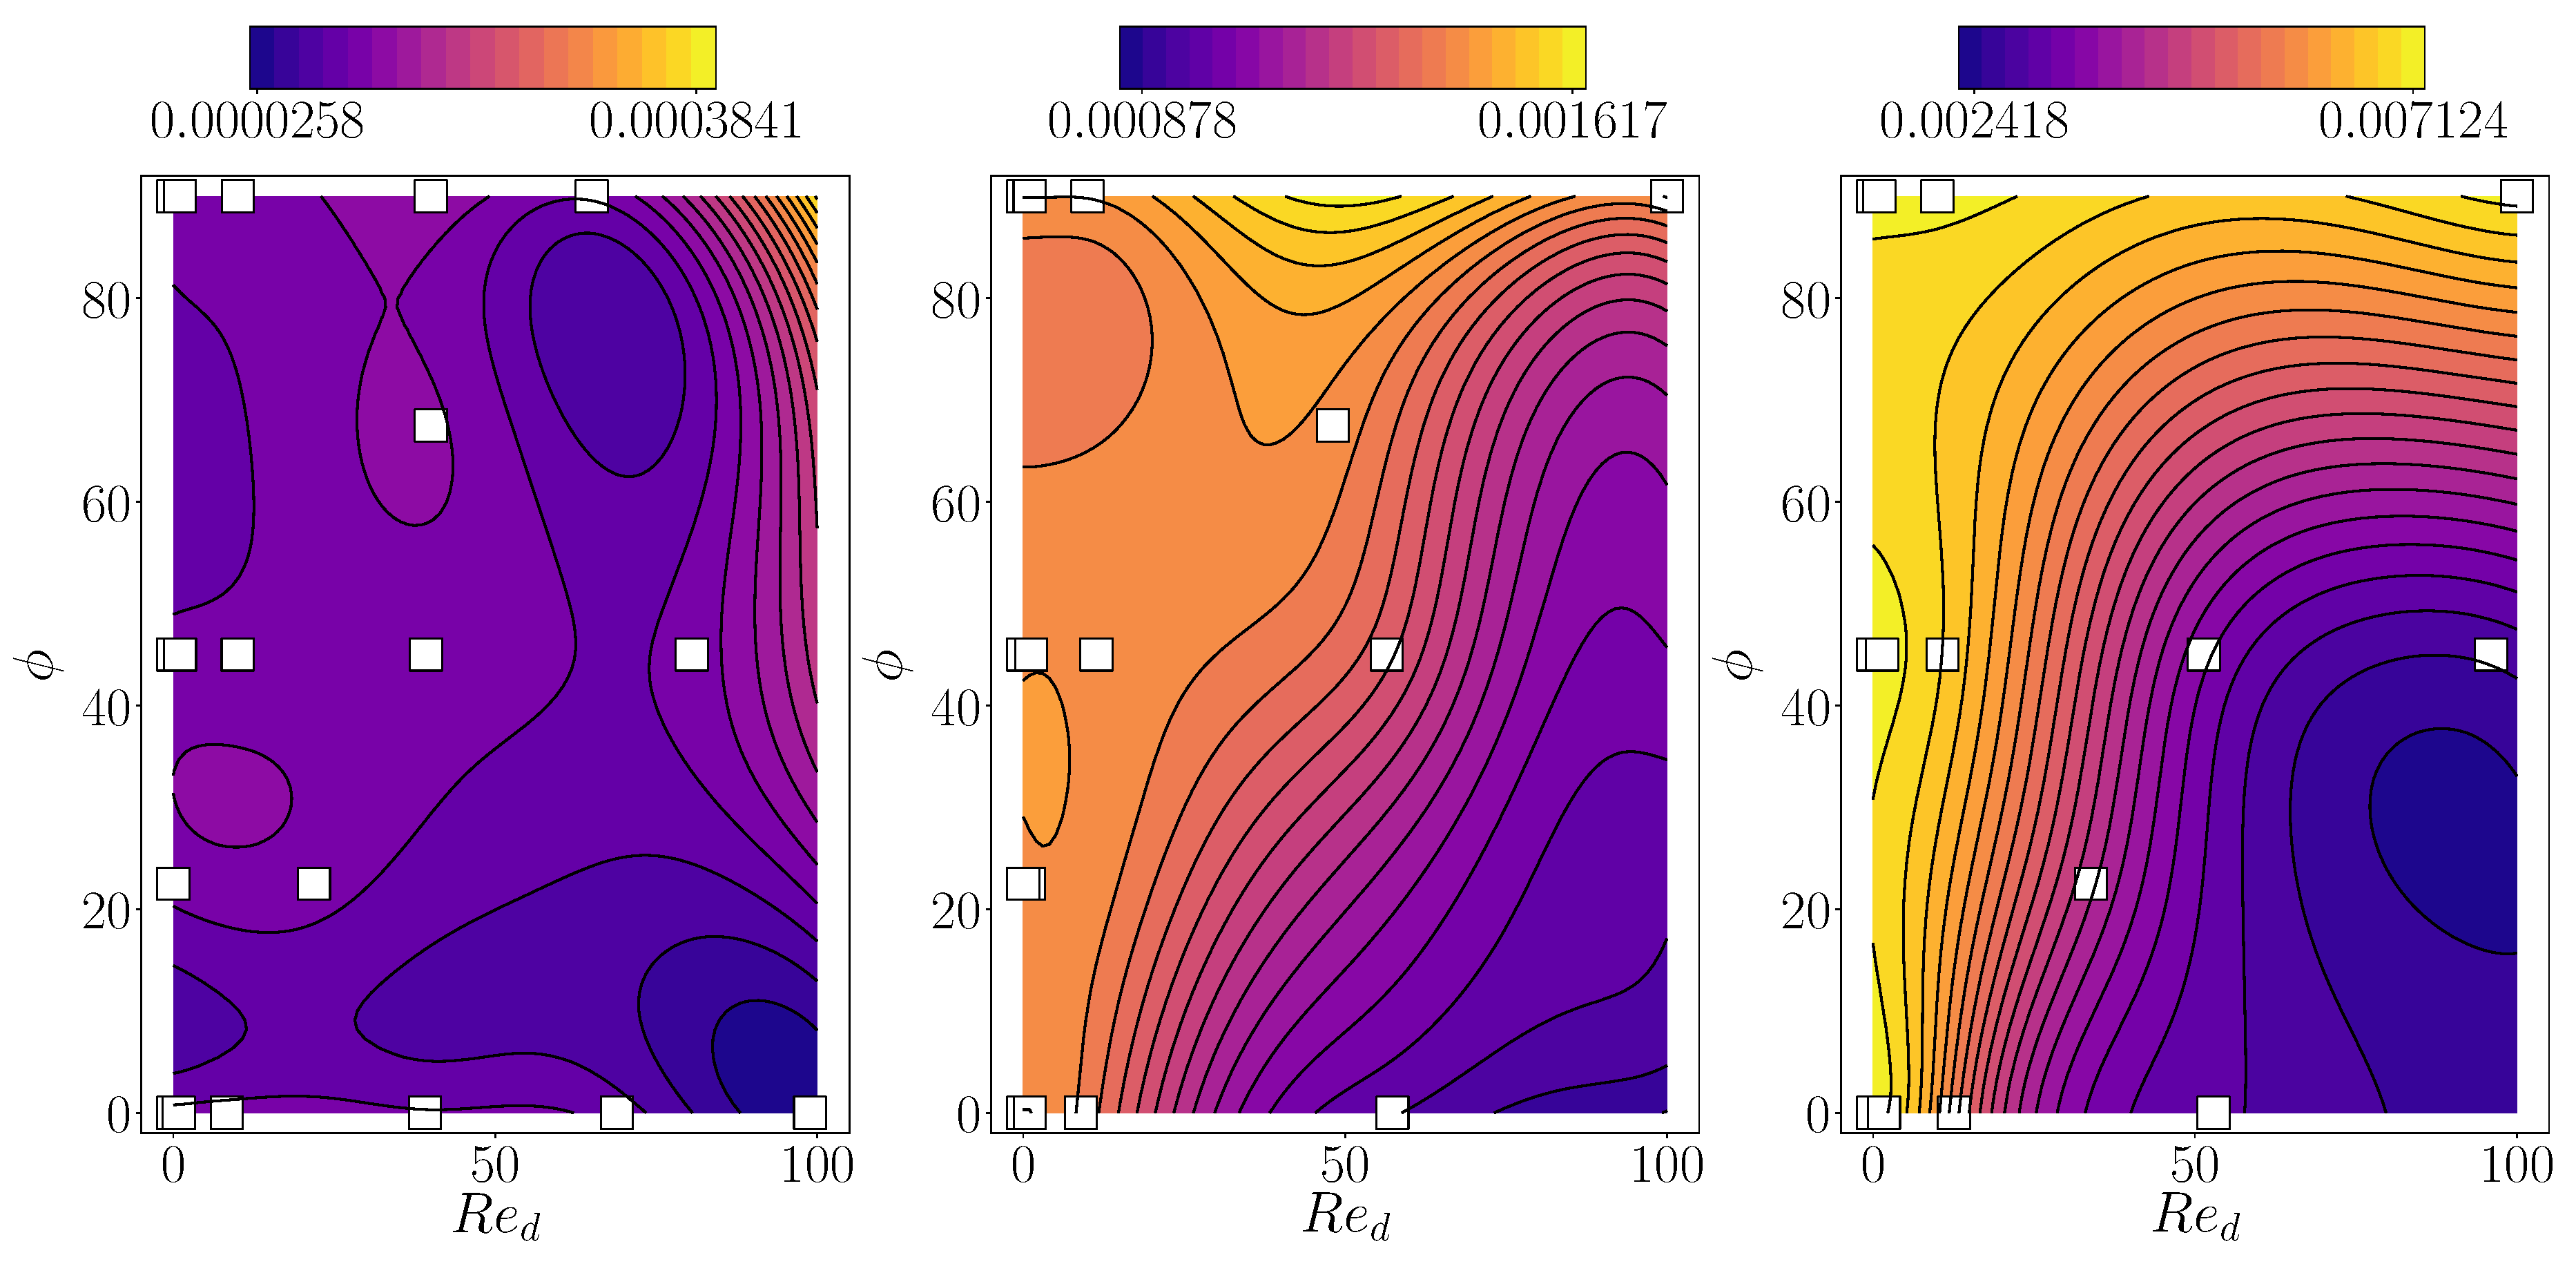
\includegraphics[width=1\linewidth]{chapter_4/figure/krig_mater_ph_re}
	\caption{Response surfaces of $H_{11}$ with $\theta=0^{\circ}$ for porosity $\varepsilon=0.4, 0.6, 0.8$, from left to right.}
	\label{fig:ph_re}
\end{figure}


In  figure \ref{fig:ph_re} the parameter  $\theta$ is set to  $0^{\circ}$ and  the response surface is displayed in the $Re_d - \phi$ plane.
As already indicated, the results confirm that an  increase of  the Reynolds number is generally associated to  a decrease of  the first diagonal component  of the apparent permeability tensor. However, the $H_{11}$ variations with respect to $\phi$ are more pronounced than those found with respect to $\theta$ and are due to a real three-dimensionalization of the flow.
This conclusion remains to be verified in the lower porosity case (left frame) where the variations are very tiny and more irregular.

%For the porosity equals to $0.8$, the surface becomes wavy  around $Re_d = 50$ region. It could be due to the lack of sampled point at this %higher range of Reynolds number. 
%In this region  the surface with porosity equals to $0.6$  shows a more regular variation. Some additional sample could help to explain the %different behaviours.




\begin{figure}[t]
	\centering
	\includegraphics[width=1\linewidth]{chapter_4/figure/krig_mater_th_phi_re40}
	\caption{Response surfaces of $H_{11}$ with $Re=40$ for porosity $\varepsilon=0.4, 0.6, 0.8$, from left to right.}
	\label{fig:th_ph}
\end{figure}


In figure \ref{fig:th_ph} the Reynolds number is set to the inertial range value of $40$ and  the response surface 
is displayed in the $\theta - \phi$ plane. 
For the two highest porosity values, $0.6$ and $0.8$, the results confirm that $H_{11}$ has a much stronger dependence on
$\phi$ than on $\theta$, suggesting that the real test of permeability models must include three-dimensional effects.
As seen earlier, the behaviour of the permeability when the porosity is low (left frame in the figure) is not intuitive, with 
a significant effect of the angle $\phi$ and a minor influence of $\theta$. Again this occurs
from the constraint provided to the flow by the inclusions, and from the occurrence of a large deviation $\gamma$ in these cases.

%shows a strong variability with respect to the angle $\phi$  and a weak one with respect to the angle $\theta$.
%At given Reynolds number the permeability does not depend (too much) of the flow direction in the horizontal plane.
%These conclusions are in agreement with the one observations written in section \ref{sec:4}.

%For the lowest porosity $0.4$ the complex behaviours are retrieved. With respect to the other porosity the variations are inverted : 
%a strong variability with respect to the angle $\theta$ and a weak one with respect to $\phi$ are found.
%As earlier  stated in the previous sections,  with a low porosity the flow direction is deflected towards the fiber axis direction with the %tri-dimensional flow.

%In the range of $\phi < 25^{\circ}$ where the tri-dimensionality remains small  the surface response exhibit a plateau in range $\theta \in %[10^\circ \  30^\circ ]$. The existence
%of this plateau remains unexplained.





The response surface is shown in the $Re_d - \varepsilon$ plane of figure \ref{fig:por} for three sets of $\theta-\phi$ angles. 
Here a significant effect of the porosity with respect to  the Reynolds number is obervable. 
In fact  the surface  gradient is almost aligned with the porosity direction, i.e. a quasi- Reynolds independence is demonstrated  in this plane,
and  the apparent permeability can change by one order of magnitude in the range
of the analysed porosity.

Some relatively small Reynolds number effects are visible at porosity equal to $0.8$, when the wake of the flow has more space to develop in the inertial regime.
In the central figure the flow is aligned with the direction of the fibers and, as expected, it shows practically no dependence with respect to the Reynolds number.


The response surface analysis has confirmed the qualitative trends which had been reached earlier on the basis of a few selected 
flow cases, yielding at the same time much more detailed information on the behaviour of the apparent permeability with the
parameters of the problem. The data base which has been built will be used in future work which will focus, via the VANS approach,
on configurations for which neither the porosity nor the local Reynolds number are constant in space or time.

\begin{figure}[t]
	\centering
	\includegraphics[width=1\linewidth]{chapter_4/figure/krig_mater_eps_re}
	\caption{Response surface of $H_{11}$; in the left frame $\phi= \theta = 0$, in the centre frame $\phi=90^{\circ}$, $ \theta = 0$ and on the right $\phi= 45^{\circ}$, $ \theta = 22.5^{\circ}$.}
	\label{fig:por}
\end{figure}


%%%%%%%%%%%%%%%%%%%%%%%%%%%%%
\section{Concluding remarks}
%%%%%%%%%%%%%%%%%%%%%%%%%%%%%


%%%%%%%%%%%%%%%%%%%%%%%%%%%%%%%%%%%%%%%%%%%%%%%%%%%%%%%%%%%%%%%%%%%%%%%%%%%%%%%%%
%\subsection{Tensors $\mathbf{K}$ and $\mathbf{F}$ by using the VANS system}
%%%%%%%%%%%%%%%%%%%%%%%%%%%%%%%%%%%%%%%%%%%%%%%%%%%%%%%%%%%%%%%%%%%%%%%%%%%%%%%%%

The components of the permeability tensor are essential ingredients for any solution of flow
through anisotropic porous media.  When the flow through the pores resents of significant
acceleration effects, the permeability must be modified (it is then called \emph{apparent}) by the presence
of a second tensor, the Forchheimer tensor $\mathbf{F}$, defined by   
$$
\mathbf{F} =  \mathbf{K} \mathbf{H}^{-1} - \mathbf{I}.
$$
The permeability, $\mathbf{K}$, and the apparent permeability, $\mathbf{H}$, can be formally deduced by two closure problems which have
been briefly recalled in section \ref{sec:2ch4}.  The real obstacle to the solution of the problem for $\mathbf{H}$ is the need
to know the microscopic velocity fields through the pores. We have solved for such fields 
in a unit cell (the REV), varying the forcing amplitude and direction, treating over one
hundred different cases of flows through arrangements of parallel fibers. From this, we have
thus been able to solve the linear system \eqref{eq:linear_k} for all the unknown elements of the 
intermediate tensor  
$\mathbf{M}$, from which, through averaging, we have computed the apparent permeability.  Such a tensor
is  indispensable to evaluate accurately the drag force caused by the presence of the fibers, for a macroscopic solution of the flow on the
basis of equations \cite{whitaker2013method} when inertial effects are present.

It has been found that the apparent permeability tensor is strongly diagonally dominant for whatever
forcing direction and porosity,  provided the local Reynolds number remains below a value 
approximately equal to 100; this results -- which is a direct
consequence of the transverse isotropy of the material which has been considered here -- 
can be used to compute $\mathbf{H}$ rapidly, approximating it as a diagonal tensor.

Finally, a metamodel has been used to produce results so as to cover the whole space of parameters,
and this has allowed the construction of a complete data base.  This data base is now being used in simulations of poroelastic media based on the VANS approach. 


%\nocite{*}  %serve per stampare tutta la bibliografia altrimenti stampa solo quella che uso nelle citazioni all'interno del testo
\bibliographystyle{plainnat}
%\bibliographystyle{unsrtnat}

\bibliography{biblio}

\end{document}